%%%%%%%%%%%%%%%%%%%%%%%%%%%%%%%%%%%%%%%%%%%%%%%%%%%%%%%%%%%%%%%%%%%%%%%%%%
%
% Generic template for TFC/TFM/TFG/Tesis at UAH
%
% $Id: book.tex,v 1.24 2019/11/29 09:31:24 macias Exp $
%
% By:
%  + Javier Macías-Guarasa.
%    Departamento de Electrónica
%    Universidad de Alcalá
%  + Roberto Barra-Chicote.
%    Departamento de Ingeniería Electrónica
%    Universidad Politécnica de Madrid
%
% Based on original sources by Roberto Barra, Manuel Ocaña, Jesús Nuevo,
% Pedro Revenga, Fernando Herránz and Noelia Hernández. Thanks a lot to
% all of them, and to the many anonymous contributors found (thanks to
% google) that provided help in setting all this up.
%
% See also the additionalContributors.txt file to check the name of
% additional contributors to this work.
%
% If you think you can add pieces of relevant/useful examples,
% improvements, please contact us at (macias@depeca.uah.es)
%
% You can freely use this template and please contribute with
% comments or suggestions!!!
%
%%%%%%%%%%%%%%%%%%%%%%%%%%%%%%%%%%%%%%%%%%%%%%%%%%%%%%%%%%%%%%%%%%%%%%%%%%%

% This is for rubber to clean additional files (do not remove!!)
% rubber: clean book.acn book.acr book.alg book.cod book.ist book.out book.sbl book.slg book.sym book.lor book.glsdefs book.loa
% rubber: onchange book.glo 'makeglossaries book'
% rubber: watch book.glo book.acr book.sym book.slg book.alg


\documentclass[spanish,openright]{book}

%%%%%%%%%%%%%%%%%%%%%%%%%%%%%%%%%%%%%%%%%%%%%%%%%%%%%%%%%%%%%%%%%%%%%%%%%%%
% BEGIN Preamble and configuration section
%
%%%%%%%%%%%%%%%%%%%%%%%%%%%%%%%%%%%%%%%%%%%%%%%%%%%%%%%%%%%%%%%%%%%%%%%%%%% 
% 
% Generic template for TFC/TFM/TFG/Tesis
% 
% $Id: preamble.tex,v 1.34 2017/04/06 13:56:12 macias Exp $
% 
% By:
% + Javier Macías-Guarasa. 
%   Departamento de Electrónica
%   Universidad de Alcalá
% + Roberto Barra-Chicote. 
%   Departamento de Ingeniería Electrónica
%   Universidad Politécnica de Madrid   
% 
% Based on original sources by Roberto Barra, Manuel Ocaña, Jesús Nuevo,
% Pedro Revenga, Fernando Herránz and Noelia Hernández. Thanks a lot to
% all of them, and to the many anonymous contributors found (thanks to
% google) that provided help in setting all this up.
% 
% See also the additionalContributors.txt file to check the name of
% additional contributors to this work.
% 
% If you think you can add pieces of relevant/useful examples,
% improvements, please contact us at (macias@depeca.uah.es)
% 
% You can freely use this template and please contribute with
% comments or suggestions!!!
% 
%%%%%%%%%%%%%%%%%%%%%%%%%%%%%%%%%%%%%%%%%%%%%%%%%%%%%%%%%%%%%%%%%%%%%%%%%%% 

%% FIXING PROBLEM WITH ALL PAGES PRINTED IN COLOR \documentclass[RGB,rgb,svgnames,spanish,openright]{book}
%\documentclass[spanish,openright]{book}
% \documentclass[english,openright]{book}
% \documentclass[11pt,english,twoside,openright]{book}

% \usepackage[a4,cam,center]{crop}
% \crop[font=\upshape\mdseries\small\textsf]

\synctex=1

% To generate a proper PDF/A document
%\usepackage[a-1b]{pdfx}

% To allow changing the default alignment of an image
\usepackage[export]{adjustbox}

% To allow simple notes to be used in the review process (see defined
% commands at the end of this file)
\usepackage{todonotes} 

% ifthen to allow using language dependent settings
\usepackage{ifthen}

%% JMG: FIXING PROBLEM WITH ALL PAGES PRINTED IN COLOR
% This should not be touched, as it should work as it is know.
\newcommand{\colorspaceused}{rgb}

%The next section seems to be useless, but it's still pending to try further
\ifthenelse{\equal{\colorspaceused}{rgb}}
{
  \PassOptionsToPackage{rgb}{xcolor}% NB: put this *before* \usepackage{pst-all}
}
{
  \PassOptionsToPackage{cmyk}{xcolor}% NB: put this *before* \usepackage{pst-all}
}

\usepackage{iftex}
%\usepackage[latin1]{inputenc} % Para poder escribir con acentos y ñ. en
                              % latin1
\ifPDFTeX
  \usepackage[utf8]{inputenc} % Para poder escribir con acentos y ñ.
  \usepackage[T1]{fontenc}      % Para que haga bien la ``hyphenation''. No
\fi                                % usar si no es necesario, porque ralentiza muchisimo la compilación.
\usepackage{ae}               % Para que todas las fuentes sean Type1, y ninguna Type3.
\usepackage{lmodern}          % This generates a pdf with searchable
                              % accented characters!!!!!!!!!!!!!!!!!!!!!!!!!!!!!!!!!!!!!!!


\usepackage{wrapfig}
\usepackage{lipsum}

% Use this if you want to include pdf files in the final document
\usepackage[final]{pdfpages}

% Use this if you want to delete headers and footers in empty pages
\usepackage{emptypage}

% \usepackage[nottoc]{tocbibind}
\usepackage{tocbibind}

\usepackage{listings}
\usepackage{longtable}
\usepackage{afterpage}

\usepackage{xspace}
\usepackage{verbatim}
\usepackage{moreverb}
\usepackage{multicol}
\usepackage{amsmath}
\usepackage{eurosym}
%\usepackage{subfig} % subfigure is obsolete... 
\usepackage{multirow}
\usepackage{fancyhdr}
\usepackage{makeidx}
\usepackage{rotating}
\usepackage{supertabular}
\usepackage{hhline}
\usepackage{array}



%% FIXING PROBLEM WITH ALL PAGES PRINTED IN COLOR
\usepackage{xcolor}
% \usepackage[RGB,rgb]{xcolor}
% \usepackage{color}
% Pantone 160
% \definecolor{headingPortadaTFM}{RGB}{158,84,10}
% Pantone 160C (this is supposed to be the correct one, but it looks horrible in screen)
% \definecolor{headingPortadaTFM}{RGB}{161,86,28}
% Gold in RGB
% \definecolor{textoHeadingPortadaTFM}{RGB}{215,215,0}
% Captured colors in screen (this looks pst on screen)

% \ifthenelse{\equal{\colorspaceused}{rgb}}
% {
%   \definecolor{headingPortadaTFM}{RGB}{152,118,52}
%   \definecolor{textoHeadingPortadaTFM}{RGB}{208,205,102}
% }
% {
%   % These definitions are for cmyk colorspace
%   \definecolor{headingPortadaTFM}{cmyk}{0.0254,0,0.559,0.537}
%   \definecolor{textoHeadingPortadaTFM}{cmyk}{0,0.0144,0.51,0.184}
% }

\definecolor{pantone293}{RGB}{35,91,168}

\definecolor{headingPortadaTFG}{RGB}{152,118,52}
\definecolor{headingPortadaTFM}{RGB}{0,90,170}
\definecolor{textoHeadingPortadaTFM}{RGB}{208,205,102}
\definecolor{textoHeadingPortadaTFG}{RGB}{208,205,102}

\definecolor{gray97}{gray}{.97}
\definecolor{gray75}{gray}{.75}
\definecolor{gray45}{gray}{.45}




% To draw rectagles in tfm cover
\usepackage{tikz}


% \usepackage[authoryear]{natbib}
% \makeatletter
% \let\NAT@parse\undefined
% \makeatother
% \usepackage{natbib}

\usepackage{geometry}
\geometry{verbose,a4paper,tmargin=2.5cm,bmargin=2.5cm,lmargin=2.5cm,rmargin=2.5cm}
% \geometry{paperwidth=210mm,paperheight=297mm}

%\usepackage[hang, flushmargin]{footmisc}   

\usepackage[
%% ps2pdf,                %%% hyper-references for ps2pdf
bookmarks=true,%                   %%% generate bookmarks ...
bookmarksnumbered=true,            %%% ... with numbers
hypertexnames=false,               %%% needed for correct links to
%%% figures!!!
% hypertexnames=true,               %%% needed for correct links on pagebackrefs!!!
breaklinks=true,                   %%% breaks lines, but links are very small
% pagebackref=true,
% linktocpage=true,                 %%% enlace en el numero de página.
linktoc=all,
colorlinks=true,
linkcolor=blue,    
citecolor=green,
urlcolor=blue,                     %%% texto  con color (further
%%% modified in myconfig.tex)
% linkbordercolor={0 0 1},           %%% blue frames around links
pdfborder={0 0 112.0},              %%% border-width of frames 
hyperfootnotes=false
]{hyperref}                        %%% will be multiplied with 0.009 by ps2pdf

\usepackage{hyperxmp}

% \usepackage[all]{hypcap}
\usepackage[center]{caption}
\usepackage{subcaption}


% Para numerar las \subsubsection
\setcounter{secnumdepth}{5}
% para hacer que las \subsubsection aparezcan en el indice
\setcounter{tocdepth}{5}
% \setcounter{lofdepth}{2}
\setcounter{table}{1}
\setcounter{figure}{1}
\setcounter{secnumdepth}{4}


\setlength{\parskip}{1ex plus 0.5ex minus 0.2ex}


\usepackage{multirow}

\usepackage{setspace}
% \renewcommand{\baselinestretch}{10}
\newcommand{\mycaptiontable}[1]{
  \begin{spacing}{0.6}
    % \vspace{0.5cm}
    \begin{quote}
      % \begin{center}
      {{Table} \thechapter.\arabic{table}: #1}
      % \end{center}
    \end{quote}
    % \vspace{1cm}
  \end{spacing}
  \stepcounter{table}
}

\newcommand{\mycaptionfigure}[1]{
  % \vspace{0.5cm}
  \begin{spacing}{0.6}
    \begin{quote}
      % \begin{center}
      {{Figure} \thechapter.\arabic{figure}: #1}
      % \end{center}
    \end{quote}
    % \vspace{1cm}
  \end{spacing}
  \stepcounter{figure}
}

\usepackage{amsmath}

\usepackage{courier}

% ***************************************************************************
% ***************************************************************************
% ***************************************************************************
\usepackage{multirow}
\usepackage{rotating}
\usepackage{setspace, amssymb, amsmath, epsfig, multirow, colortbl, tabularx}%
% For acronym package:
% If footnote is specified, text will be included in a footnote
% If printonlyused is specified, only used acronyms will be included
% I use the acronym sty under the sty directory as I needed the newest version
% \usepackage[footnote,printonlyused,withpage]{acronym} 
% \usepackage[printonlyused]{sty/acronym}

% glossaries is better than the acronym package 
\usepackage[automake,acronym,shortcuts,nomain,hyperfirst=false]{glossaries}
% If you want to PERMANENTLY DISABLE HYPERLINKS, uncomment the following
% line
% \glsdisablehyper
% In future versiones (not as for ubuntu 12.04) You can also selectively
% disable hyperlinks for given glossaries, using:
% \usepackage[acronym,shortcuts,nomain,nohypertypes={acronyms,symbols}]{glossaries}
% Or (for newwer versions also), you can even use
% \GlsDeclareNoHyperList{acronyms,symbols}
% You can also disable hyperlinks in the acronym use, like in \ac*{symbol}


\newcommand{\clearemptydoublepage}{\newpage{\pagestyle{empty}\cleardoublepage}}

\pagestyle{fancy}

\providecommand\phantomsection{}
\onehalfspacing
\sloppy  %better line breaks

\renewcommand{\chaptermark}[1]{\markboth{\chaptername\ \thechapter.\ #1}{}}
\renewcommand{\sectionmark}[1]{\markright{\thesection\ #1}{}}

%%%%%%%%%%%%%%%%%%%%%%%%%%%%%%%%%%%%%%%%%%%%%%%%%%%%%%%%%%%%%%%%%%%%%%%%%%% 
% BEGIN Fancy headers stuff
\fancyhf{}

\fancyhead[LE,RO]{\bfseries\thepage}
\fancyhead[LO]{\bfseries\rightmark}
\fancyhead[RE]{\bfseries\leftmark}

\makeatletter
\renewcommand{\chaptermark}[1]{\markboth{\@chapapp \ \thechapter . \ #1}{}}
\renewcommand{\sectionmark}[1]{\markright{\thesection \ \ #1}}
\makeatother

\renewcommand{\headrulewidth}{0.5pt}
\renewcommand{\footrulewidth}{0pt}
\addtolength{\headheight}{3.5pt}
\fancypagestyle{plain}{\fancyhead{}\renewcommand{\headrulewidth}{0pt}}
\fancypagestyle{myplain}
{
  \fancyhf{}
  \renewcommand\headrulewidth{0pt}
  \renewcommand\footrulewidth{0pt}
  \fancyfoot[C]{\thepage}
}
% END Fancy headers stuff
%%%%%%%%%%%%%%%%%%%%%%%%%%%%%%%%%%%%%%%%%%%%%%%%%%%%%%%%%%%%%%%%%%%%%%%%%%% 

%%%%%%%%%%%%%%%%%%%%%%%%%%%%%%%%%%%%%%%%%%%%%%%%%%%%%%%%%%%%%%%%%%%%%%%%%%% 
% BEGIN Set nice chapter titles

% BEGIN Example 0 from http://texblog.org/2012/07/03/fancy-latex-chapter-styles/
% \usepackage[explicit]{titlesec}
% \usepackage{blindtext}
% \definecolor{gray75}{gray}{0.75}
% \newcommand{\hsp}{\hspace{20pt}}
% \titleformat{\chapter}[hang]{\Huge\bfseries}{\chaptername~\thechapter\hsp\textcolor{gray75}{|}\hsp}{0pt}{\Huge\bfseries}
% END Example 0 from http://texblog.org/2012/07/03/fancy-latex-chapter-styles/

% BEGIN Example 1 from http://texblog.org/2012/07/03/fancy-latex-chapter-styles/
% \usepackage{titlesec}
% \usepackage{blindtext}
% \definecolor{gray75}{gray}{0.75}
% \newcommand{\hsp}{\hspace{20pt}}
% \titleformat{\chapter}[hang]{\Huge\bfseries}{\chaptername~\thechapter\hsp\textcolor{gray75}{|}\hsp}{0pt}{\Huge\bfseries}
% END Example 1 from http://texblog.org/2012/07/03/fancy-latex-chapter-styles/

% BEGIN Example 2 from http://texblog.org/2012/07/03/fancy-latex-chapter-styles/
% Options: Sonny, Lenny, Glenn, Conny, Rejne, Bjarne, Bjornstrup
% \usepackage[Sonny]{fncychap}
% \usepackage[Lenny]{fncychap} % ugly
% \usepackage[Glenn]{fncychap}
% \usepackage[Conny]{fncychap} % ugly
% \usepackage[Rejne]{fncychap}
% \usepackage[Bjarne]{fncychap} % Doesn't work in Spanish
% \usepackage[Bjornstrup]{fncychap}
% END   Example 2 from http://texblog.org/2012/07/03/fancy-latex-chapter-styles/

% BEGIN Example 3 from http://texblog.org/2012/07/03/fancy-latex-chapter-styles/
% This is a nice colored example
% \usepackage{kpfonts}
% \usepackage[explicit]{titlesec}
% \newcommand*\chapterlabel{}
% \titleformat{\chapter}
% {\gdef\chapterlabel{}
% \normalfont\sffamily\Huge\bfseries\scshape}
% {\gdef\chapterlabel{\thechapter\ }}{0pt}
% {\begin{tikzpicture}[remember picture,overlay]
%   \node[yshift=-3cm] at (current page.north west)
%   {\begin{tikzpicture}[remember picture, overlay]
%     \draw[fill=LightSkyBlue] (0,0) rectangle
%     (\paperwidth,3cm);
%     \node[anchor=east,xshift=.9\paperwidth,rectangle,
%     rounded corners=20pt,inner sep=11pt,
%     fill=MidnightBlue]
%     {\color{white}\chapterlabel#1};
%   \end{tikzpicture}
% };
% \end{tikzpicture}
% }
%   \titlespacing*{\chapter}{0pt}{50pt}{-60pt}
%   END   Example 3 from http://texblog.org/2012/07/03/fancy-latex-chapter-styles/

%   BEGIN Example 4 from http://texblog.org/2012/07/03/fancy-latex-chapter-styles/
%   END   Example 4 from http://texblog.org/2012/07/03/fancy-latex-chapter-styles/


%   END Set nice chapter titles
%%%%%%%%%%%%%%%%%%%%%%%%%%%%%%%%%%%%%%%%%%%%%%%%%%%%%%%%%%%%%%%%%%%%%%%%%%%   

%%%%%%%%%%%%%%%%%%%%%%%%%%%%%%%%%%%%%%%%%%%%%%%%%%%%%%%%%%%%%%%%%%%%%%%%%%%   
%   This is to set background images (in our case to set background image
%   in TFMs front and back pages)
%   If you want to set this background, use \BgThispage in the
%   corresponding pages
%\usepackage[pages=some]{sty/background}
\usepackage[pages=some]{background}

% Note that we also set the opacity in the first page of the tfg due to a bug,
% so it you modify it here remember to modify the value in Book/cover/portada-tfm-uah.tex
% https://tex.stackexchange.com/questions/649514/how-to-produce-a-transparent-image-with-xelatex/649518#649518
% https://tex.stackexchange.com/questions/640574/using-a-tikzpicture-disables-opacity-for-first-bgthispage-how-can-i-fix-this
\ifthenelse{\equal{\colorspaceused}{rgb}}
{
  \backgroundsetup{ scale=1, angle=0, opacity=.1, color=pink,
    contents={
\includegraphics[width=.7\paperwidth]{logos/logoEPS-UAH.jpg}}, vshift=-50pt,  hshift=0pt }
}
{
  \backgroundsetup{ scale=1, angle=0, opacity=.1, color=pink,
    contents={
\includegraphics[width=.7\paperwidth]{logos/logoEPS-UAH-cmyk.jpg}}, vshift=-50pt,  hshift=0pt }
}


% This is to allow do a clearpage and let the next one to be placed in
% even pages (to set a backpage for example)
\makeatletter
\newcommand*{\cleartoleftpage}{%
  \clearpage
  \if@twoside
  \ifodd\c@page
  \hbox{}\newpage
  \if@twocolumn
  \hbox{}\newpage
  \fi
  \fi
  \fi
}
\makeatother

% Let's define some styles for source code listings:
% 
% minimizar fragmentado de listados (from
% http://www.rafalinux.com/?p=599), pero no me funciona:
% \lstnewenvironment{codelisting}[1][]
% {\lstset{#1}\pagebreak[0]}{\pagebreak[0]}
% 
% This was using the float package
\usepackage{float}
\floatstyle{plaintop} % optionally change the style of the new float
\newfloat{codefloat}{H}{cod}[chapter]

% Support utf-8 in listings. 
% The way the inputenc package works with non-ASCII UTF-8-encoded characters (by
% making the first byte active and then reading the following ones as arguments)
% is fundamentally incompatible with the way the listing package works, which
% reads each byte individually and expects it to be an individual character.
% See https://tex.stackexchange.com/questions/24528/having-problems-with-listings-and-utf-8-can-it-be-fixed
\lstset{
    inputencoding = utf8,  % Input encoding
    extendedchars = true,  % Extended ASCII
    literate      =        % Support additional characters
      {á}{{\'a}}1  {é}{{\'e}}1  {í}{{\'i}}1 {ó}{{\'o}}1  {ú}{{\'u}}1
      {Á}{{\'A}}1  {É}{{\'E}}1  {Í}{{\'I}}1 {Ó}{{\'O}}1  {Ú}{{\'U}}1
      {à}{{\`a}}1  {è}{{\`e}}1  {ì}{{\`i}}1 {ò}{{\`o}}1  {ù}{{\`u}}1
      {À}{{\`A}}1  {È}{{\'E}}1  {Ì}{{\`I}}1 {Ò}{{\`O}}1  {Ù}{{\`U}}1
      {ä}{{\"a}}1  {ë}{{\"e}}1  {ï}{{\"i}}1 {ö}{{\"o}}1  {ü}{{\"u}}1
      {Ä}{{\"A}}1  {Ë}{{\"E}}1  {Ï}{{\"I}}1 {Ö}{{\"O}}1  {Ü}{{\"U}}1
      {â}{{\^a}}1  {ê}{{\^e}}1  {î}{{\^i}}1 {ô}{{\^o}}1  {û}{{\^u}}1
      {Â}{{\^A}}1  {Ê}{{\^E}}1  {Î}{{\^I}}1 {Ô}{{\^O}}1  {Û}{{\^U}}1
      {œ}{{\oe}}1  {Œ}{{\OE}}1  {æ}{{\ae}}1 {Æ}{{\AE}}1  {ß}{{\ss}}1
      {ç}{{\c c}}1 {Ç}{{\c C}}1 {ø}{{\o}}1  {Ø}{{\O}}1   {å}{{\r a}}1
      {Å}{{\r A}}1 {ã}{{\~a}}1  {õ}{{\~o}}1 {Ã}{{\~A}}1  {Õ}{{\~O}}1
      {ñ}{{\~n}}1  {Ñ}{{\~N}}1  {¿}{{?`}}1  {¡}{{!`}}1
      {°}{{\textdegree}}1 {º}{{\textordmasculine}}1 {ª}{{\textordfeminine}}1
      % ¿ and ¡ are not correctly displayed if inconsolata font is used
      % together with the lstlisting environment. Consider typing code in
      % external files and using \lstinputlisting to display them instead.      
  }

\lstdefinestyle{console}
{
  basicstyle=\scriptsize\bf\ttfamily,
  backgroundcolor=\color{gray75},
}

\lstdefinestyle{Cbluebox}
{
  language=C,
  frame=shadowbox, 
  rulesepcolor=\color{blue}
}

\lstdefinestyle{Cnice}
{
  language=C,
  frame=Ltb,
  framerule=0pt,
  tabsize=2,
  aboveskip=0.5cm,
  framextopmargin=3pt,
  framexbottommargin=3pt,
  framexleftmargin=0.4cm,
  framesep=0pt,
  rulesep=.4pt,
  backgroundcolor=\color{gray97},
  rulesepcolor=\color{black},
  % 
  stringstyle=\ttfamily,
  showstringspaces = false,
  % basicstyle=\small\ttfamily,
  basicstyle=\footnotesize\ttfamily,
  commentstyle=\color{gray45},
  keywordstyle=\bfseries,
  % 
  numbers=left,
  numbersep=15pt,
  numberstyle=\tiny,
  numberfirstline = false,
  breaklines=true,
}	

\lstdefinestyle{CppExample}
{
  language=C++,
  frame=trbl,
  tabsize=2,
  commentstyle=\textit,
  stringstyle=\ttfamily, 
  basicstyle=\small,
}	

% This one from http://en.wikibooks.org/wiki/LaTeX/Source_Code_Listings
\lstdefinestyle{Ccolor}
{
  belowcaptionskip=1\baselineskip,
  breaklines=true,
  frame=L,
  xleftmargin=\parindent,
  language=C,
  showstringspaces=false,
  basicstyle=\footnotesize\ttfamily,
  keywordstyle=\bfseries\color{green!40!black},
  commentstyle=\itshape\color{purple!40!black},
  identifierstyle=\color{blue},
  stringstyle=\color{orange},
}

% From http://tex.stackexchange.com/questions/46953/unix-command-highlighting-latex
\lstdefinestyle{BashInputStyle}{
  language=bash,
  basicstyle=\small\sffamily,
  numbers=left,
  numberstyle=\tiny,
  numbersep=3pt,
  frame=tb, 
  showspaces=false, 
  showtabs=false,
  showstringspaces=false,
  columns=fullflexible,
  backgroundcolor=\color{gray97},
  % backgroundcolor=\color{yellow!20},
  linewidth=0.9\linewidth,
  xleftmargin=0.05\linewidth
}

\definecolor{mGreen}{rgb}{0,0.6,0}
\definecolor{mGray}{rgb}{0.5,0.5,0.5}
\definecolor{mPurple}{rgb}{0.58,0,0.82}
\definecolor{backgroundColour}{rgb}{0.95,0.95,0.92}

\lstdefinestyle{CStyle}{
    backgroundcolor=\color{backgroundColour},   
    commentstyle=\color{mGreen},
    keywordstyle=\color{magenta},
    numberstyle=\tiny\color{mGray},
    stringstyle=\color{mPurple},
    basicstyle=\footnotesize,
    breakatwhitespace=false,         
    breaklines=true,                 
    captionpos=b,                    
    keepspaces=true,                 
    numbers=left,                    
    numbersep=5pt,                  
    showspaces=false,                
    showstringspaces=false,
    showtabs=false,                  
    tabsize=2,
    language=C
}

\lstdefinestyle{BashStyle}{
    backgroundcolor=\color{backgroundColour},   
    commentstyle=\color{mGreen},
    keywordstyle=\color{magenta},
    numberstyle=\tiny\color{mGray},
    stringstyle=\color{mPurple},
    basicstyle=\footnotesize,
    breakatwhitespace=false,         
    breaklines=true,                 
    captionpos=b,                    
    keepspaces=true,                 
    numbers=left,                    
    numbersep=5pt,                  
    showspaces=false,                
    showstringspaces=false,
    showtabs=false,                  
    tabsize=2,
    language=bash
}

\lstdefinestyle{Bashnice}
{
  language=bash,
  frame=Ltb,
  framerule=0pt,
  tabsize=2,
  aboveskip=0.5cm,
  framextopmargin=3pt,
  framexbottommargin=3pt,
  framexleftmargin=0.4cm,
  framesep=0pt,
  rulesep=.4pt,
  backgroundcolor=\color{gray97},
  rulesepcolor=\color{black},
  % 
  stringstyle=\ttfamily,
  showstringspaces = false,
  % basicstyle=\small\ttfamily,
  basicstyle=\footnotesize\ttfamily,
  commentstyle=\color{gray45},
  keywordstyle=\bfseries,
  % 
  numbers=left,
  numbersep=15pt,
  numberstyle=\tiny,
  numberfirstline = false,
  breaklines=true,
}	


% To set side-captions in figures
\usepackage{sidecap}

%%%%%%%%%%%%%%%%%%%%%%%%%%%%%%%%%%%%%%%%%%%%%%%%%%%%%%%%%%%%%%%%%%%%%%%%%%% 
% This comes from TeXiS, thanks to its authors, available at
% http://gaia.fdi.ucm.es/projects/texis 
\def\texis{\TeX \raise.15em\hbox{\textsc{i}}S}
%%%%%%%%%%%%%%%%%%%%%%%%%%%%%%%%%%%%%%%%%%%%%%%%%%%%%%%%%%%%%%%%%%%%%% 
% Comando:
% 
% \begin{FraseCelebre}
%   \begin{Frase}
%     Y así, del mucho leer y del poco dormir...
%   \end{Frase}
%   \begin{Fuente}
%     Don Quijote de la Mancha
%     
%     Miguel de Cervantes
%   \end{Fuente}
%   \begin{FraseCelebre}
%     
%     Resultado:
%     
%     Añade la frase célebre del principio de un capítulo.
%%%%%%%%%%%%%%%%%%%%%%%%%%%%%%%%%%%%%%%%%%%%%%%%%%%%%%%%%%%%%%%%%%%%%%     
\newenvironment{FraseCelebre}% Definición del entorno de FraseCelebre
{\begin{list}{}{%
      \setlength{\leftmargin}{0.5\textwidth}% Desplazamos el inicio de
      % los párrafos a la derecha la mitad
      % de la anchura de la línea de texto.
      % Puede que quieras cambiar esto
      % por otra cantidad como '5cm'.
      \setlength{\parsep}{0cm}% La separación entre párrafos de la
      % frase o de la fuente es normal, sin
      % espacio extra.
      \addtolength{\topsep}{0.5cm}% Aumentamos un poco la separación
      % entre la parte de la fase célebre
      % y los párrafos de alrededor
    }
  }
  {\unskip \end{list}}

\newenvironment{Frase}%
{\item \begin{flushright}\small\em}%
  {\end{flushright}}

\newenvironment{Fuente}%
{\item \begin{flushright}\small}%
  {\end{flushright}}


% To put paragraphs at page bottom
\newenvironment{bottomparagraph}{\par\vspace*{\fill}}{\clearpage}
% \newenvironment{bottomparagraph}{\par\vspace*{\fill}}{\clearemptydoublepage}

% Add algorithms april 2014
\usepackage[vlined,algochapter]{algorithm2e}
% Make this compatible with older/newer versions of the package
\providecommand{\DontPrintSemicolon}{\dontprintsemicolon}
\providecommand{\SetAlgoLined}{\SetLine}



% Add support for fonts at arbitrary sizes september 2014, for TFG's cover
\usepackage{fix-cm}

\usepackage{graphicx}                                                                      

% This is to avoid producing an hyperlink for starred documents. ONLY
% WORKS FOR THE ACRONYM PACKAGE, NOT USED HERE ANYMORE
% \makeatletter
% \AtBeginDocument{%
%   \renewcommand*\AC@hyperlink{%
%     \ifAC@starred
%       \expandafter\@secondoftwo
%     \else
%       \expandafter\hyperlink
%     \fi
%   }%
% }
% \makeatother

% This should be relative to the book.tex path, do not touch!!!!!!!!!!!
\newcommand{\myreferencespath}{}

%\providecommand{\DIFadd}[1]{{\protect\color{blue}#1}} %DIF PREAMBLE
%\providecommand{\DIFdel}[1]{{\protect\color{red}\protect\scriptsize{#1}}}

% As fancy underlining does not seem to compile with pdflatex, remove underline
%\providecommand{\DIFadd}[1]{{\protect\color{blue}{\protect\uwave{#1}}}}
%\providecommand{\DIFadd}[1]{{\protect\color{blue}\textbf{#1}}}
\providecommand{\DIFdel}[1]{{\protect\color{red}\sout{#1}}}                     


%%%%%%%%%%%%%%%%%%%%%%%%%%%%%%%%%%%%%%%%%%%%%%%%%%%%%%%%%%%%%%%%%%%%%%%%%%%
% 
\usepackage{ifpdf}
\ifpdf
  \DeclareGraphicsExtensions{.pdf,.png,.jpg}
\else
  \DeclareGraphicsExtensions{.eps}
\fi

\DeclareGraphicsExtensions{.pdf,.png,.jpg}


%%%%%%%%%%%%%%%%%%%%%%%%%%%%%%%%%%%%%%%%%%%%%%%%%%%%%%%%%%%%%%%%%%%%%%%%%%%
% Para control de viudas y huérfanas
\clubpenalty=10000
\widowpenalty=10000


%%%%%%%%%%%%%%%%%%%%%%%%%%%%%%%%%%%%%%%%%%%%%%%%%%%%%%%%%%%%%%%%%%%%%%%%%%%
% As requested by Carlos Cruz on August 2020 To make "Appendix X
% Appendix title" in TOC instead of simply "X Appendix title" (from
% https://tex.stackexchange.com/questions/44858/adding-the-word-appendix-to-table-of-contents-in-latex/44971
% and
% https://tex.stackexchange.com/questions/58848/ap%C3%A9ndices-appendix-spanish-accent):
\usepackage[titletoc]{appendix}
\usepackage{etoolbox}
\makeatletter
\appto{\appendices}{\def\Hy@chapapp{Appendix}}
\makeatother


%%%%%%%%%%%%%%%%%%%%%%%%%%%%%%%%%%%%%%%%%%%%%%%%%%%
% Bibliography backend control. It is recommended  that we use biblatex, as it
% supports more keys (for example, when we cite a website we can specify the
% visited date, in the .bib file). It also support multiple files more easily
% and more bibliography styles

% \newcommand{\bibliosystem}{bibtex} % Valid options are biblatex or bibtex
\newcommand{\bibliosystem}{biblatex} % Valid options are biblatex or bibtex

\ifthenelse{\equal{\bibliosystem}{biblatex}}
{
  % Suggestion by Miguel Cubero (2023)
  % When using babel or polyglossia with biblatex, loading csquotes is
  % recommended to ensure that quoted texts are typeset according to the
  % rules of your main language.

  \usepackage{csquotes}

  % Use biblatex instead of bibtex
  \usepackage[backend=biber,style=ieee]{biblatex}
  % This is a dirty hack, but should work... The reason to do so is to avoid
  % the need of editing this file by the user (see Book/biblio files for more
  % details)
  %% Here define as many bibfiles as needed
%%
%% It is compulsory that they are named as \mybibfileOne
%% \mybibfileTwo, \mybibfileThree, ... \mybibfileTen
%%
%% If you need more than ten, you will have to edit
%% Config/preamble.tex and Book/biblio/bibliography.tex
%% to support this adition
%%
%% The file names may change at your will, but they must
%% be in the Book/biblio directory

\newcommand{\mybibfileOne}{biblio/biblio.bib}
\newcommand{\mybibfileTwo}{biblio/nobiblio.bib}
%% \newcommand{\mybibfileThree}{AudioVisualNew.bib}
%% \newcommand{\mybibfileFour}{biblio/audiotracking.bib}
%% \newcommand{\mybibfileFive}{biblio/audiovisualtracking.bib}
%% \newcommand{\mybibfileSix}{biblio/backgroungsubstraction.bib}
%% \newcommand{\mybibfileSeven}{biblio/databases.bib}
%% \newcommand{\mybibfileEight}{biblio/evalmetrics.bib}
%% \newcommand{\mybibfileNine}{biblio/facedetect.bib}
%% \newcommand{\mybibfileTen}{biblio/facedetectADABOOST.bib}
%% \newcommand{\mybibfileEleven}{biblio/facedetectmultiview.bib}
%% \newcommand{\mybibfileTwelve}{biblio/facedetectprob2d.bib}
%% \newcommand{\mybibfileThirteen}{biblio/others.bib}
%% \newcommand{\mybibfileFourteen}{biblio/skindetect.bib}
%% \newcommand{\mybibfileFifteen}{biblio/tracking.bib}
%% \newcommand{\mybibfileSixteen}{biblio/videotracking.bib}
%% \newcommand{\mybibfileSeventeen}{biblio/voiceActivityDetection.bib}
%% \newcommand{\mybibfileEighteen}{biblio/headposeextraction.bib}
%% \newcommand{\mybibfileNineteen}{biblio/AudioVisualSpeakerTracking.bib}
%% \newcommand{\mybibfileTwenty}{biblio/BibliogPFVJ.bib}
%% \newcommand{\mybibfileTwentyone}{biblio/tools.bib}
%% \newcommand{\mybibfileTwentytwo}{biblio/infrared.bib}
%% \newcommand{\mybibfileTwentythree}{}
%% \newcommand{\mybibfileTwentyfour}{}
%% \newcommand{\mybibfileTwentyfive}{}



  \ifdef{\mybibfileOne}
  {
    \addbibresource{\myreferencespath\mybibfileOne}
  }
  {
    \errorYOUmustDEFINEatLEASTmybibfileOneInbibliofilesDOTtex
  }
  \ifdef{\mybibfileTwo}
  {
    \addbibresource{\myreferencespath\mybibfileTwo}
  }
  {
  }
  \ifdef{\mybibfileThree}
  {
    \addbibresource{\myreferencespath\mybibfileThree}
  }
  {
  }
  \ifdef{\mybibfileFour}
  {
    \addbibresource{\myreferencespath\mybibfileFour}
  }
  {
  }
  \ifdef{\mybibfileFive}
  {
  \addbibresource{\myreferencespath\mybibfileFive}
  }
  {
  }
  \ifdef{\mybibfileSix}
  {
    \addbibresource{\myreferencespath\mybibfileSix}
  }
  {
  }

  \ifdef{\mybibfileSeven}
  {
    \addbibresource{\myreferencespath\mybibfileSeven}
  }
  {
  }
  \ifdef{\mybibfileEight}
  {
    \addbibresource{\myreferencespath\mybibfileEight}
  }
  {
  }

  \ifdef{\mybibfileNine}
  {
    \addbibresource{\myreferencespath\mybibfileNine}
  }
  {
  }

  \ifdef{\mybibfileTen}
  {
    \addbibresource{\myreferencespath\mybibfileTen}
  }
  {
  }

  \ifdef{\mybibfileEleven}
  {
    \addbibresource{\myreferencespath\mybibfileEleven}
  }
  {
  }

  \ifdef{\mybibfileTwelve}
  {
    \addbibresource{\myreferencespath\mybibfileTwelve}
  }
  {
  }

  \ifdef{\mybibfileThirteen}
  {
    \addbibresource{\myreferencespath\mybibfileThirteen}
  }
  {
  }

  \ifdef{\mybibfileFourteen}
  {
    \addbibresource{\myreferencespath\mybibfileFourteen}
  }
  {
  }

  \ifdef{\mybibfileFifteen}
  {
    \addbibresource{\myreferencespath\mybibfileFifteen}
  }
  {
  }

  \ifdef{\mybibfileSixteen}
  {
    \addbibresource{\myreferencespath\mybibfileSixteen}
  }
  {
  }

  \ifdef{\mybibfileSeventeen}
  {
    \addbibresource{\myreferencespath\mybibfileSeventeen}
  }
  {
  }

  \ifdef{\mybibfileEighteen}
  {
    \addbibresource{\myreferencespath\mybibfileEighteen}
  }
  {
  }

  \ifdef{\mybibfileNineteen}
  {
    \addbibresource{\myreferencespath\mybibfileNineteen}
  }
  {
  }

  \ifdef{\mybibfileTwenty}
  {
    \addbibresource{\myreferencespath\mybibfileTwenty}
  }
  {
  }

  \ifdef{\mybibfileTwentyone}
  {
    \addbibresource{\myreferencespath\mybibfileTwentyone}
  }
  {
  }

  \ifdef{\mybibfileTwentytwo}
  {
    \addbibresource{\myreferencespath\mybibfileTwentytwo}
  }
  {
  }

  \ifdef{\mybibfileTwentythree}
  {
    \addbibresource{\myreferencespath\mybibfileTwentythree}
  }
  {
  }

  \ifdef{\mybibfileTwentyfour}
  {
    \addbibresource{\myreferencespath\mybibfileTwentyfour}
  }
  {
  }

  \ifdef{\mybibfileTwentyfive}
  {
    \addbibresource{\myreferencespath\mybibfileTwentyfive}
  }
  {
  }

}
{
  % Use bibtex
  \usepackage[noadjust]{cite}      % Written by Donald Arseneau
  % V1.6 and later of IEEEtran pre-defines the format
  % of the cite.sty package \cite{} output to follow
  % that of IEEE. Loading the cite package will
  % result in citation numbers being automatically
  % sorted and properly "ranged". i.e.,
  % [1], [9], [2], [7], [5], [6]
  % (without using cite.sty)
  % will become:
  % [1], [2], [5]--[7], [9] (using cite.sty)
  % cite.sty's \cite will automatically add leading
  % space, if needed. Use cite.sty's noadjust option
  % (cite.sty V3.8 and later) if you want to turn this
  % off. cite.sty is already installed on most LaTeX
  % systems. The latest version can be obtained at:
  % http://www.ctan.org/tex-archive/macros/latex/contrib/supported/cite/
}


% From https://tex.stackexchange.com/questions/50830/do-i-have-to-care-about-bad-boxes/50850#50850
% To hide warning messages about slightly overfilled paragraphs
% This should not be here but I want to avoid adding extra files to do tiny things...
\hfuzz=2pt
\vfuzz=2pt

% For centering columns in tables
\usepackage{array}

\usepackage{bera}% optional: just to have a nice mono-spaced font
\usepackage{listings}
\usepackage{xcolor}

\colorlet{punct}{red!60!black}
\definecolor{background}{HTML}{EEEEEE}
\definecolor{delim}{RGB}{20,105,176}
\colorlet{numb}{magenta!60!black}

\lstdefinelanguage{json}{
    basicstyle=\normalfont\ttfamily,
    numbers=left,
    numberstyle=\scriptsize,
    stepnumber=1,
    numbersep=8pt,
    showstringspaces=false,
    breaklines=true,
    frame=lines,
    backgroundcolor=\color{background},
    literate=
     *{0}{{{\color{numb}0}}}{1}
      {1}{{{\color{numb}1}}}{1}
      {2}{{{\color{numb}2}}}{1}
      {3}{{{\color{numb}3}}}{1}
      {4}{{{\color{numb}4}}}{1}
      {5}{{{\color{numb}5}}}{1}
      {6}{{{\color{numb}6}}}{1}
      {7}{{{\color{numb}7}}}{1}
      {8}{{{\color{numb}8}}}{1}
      {9}{{{\color{numb}9}}}{1}
      {:}{{{\color{punct}{:}}}}{1}
      {,}{{{\color{punct}{,}}}}{1}
      {\{}{{{\color{delim}{\{}}}}{1}
      {\}}{{{\color{delim}{\}}}}}{1}
      {[}{{{\color{delim}{[}}}}{1}
      {]}{{{\color{delim}{]}}}}{1},
}


%For making Gantt diagrams
\usepackage{pgfgantt}

\usepackage{lscape}
\usepackage{rotating}

\usepackage{dirtree}

\usepackage{mathtools}
\DeclarePairedDelimiter\bra{\langle}{\rvert}
\DeclarePairedDelimiter\ket{\lvert}{\rangle}

% Some TFG/TFM regulations state that double spacing should be used In my
% opinion it is obsolete and ugly, but if you want to do so, add the following
% command here:
% \renewcommand{\baselinestretch}{2}

% Some TFG/TFM regulations state that Arial font should be used. In my
% opinion the LaTeX standard fornt is better, but if you want to do so, use Helvetica instead (Arial is not free) adding the following commands here:
% \usepackage{helvet}
% \renewcommand{\familydefault}{\sfdefault}


%%% Local Variables:
%%% TeX-master: "../book"
%%% End:


    % DO NOT TOUCH THIS LINE. You can edit
                               % the file to modify some default settings

%%%%%%%%%%%%%%%%%%%%%%%%%%%%%%%%%%%%%%%%%%%%%%%%%%%%%%%%%%%%%%%%%%%%%%%%%%%
%
% Generic template for TFC/TFM/TFG/Tesis
%
% $Id: myconfig.tex,v 1.39 2020/03/24 17:33:24 macias Exp $
%
% By:
%  + Javier Macías-Guarasa. 
%    Departamento de Electrónica
%    Universidad de Alcalá
%  + Roberto Barra-Chicote. 
%    Departamento de Ingeniería Electrónica
%    Universidad Politécnica de Madrid   
% 
% Based on original sources by Roberto Barra, Manuel Ocaña, Jesús Nuevo,
% Pedro Revenga, Fernando Herránz and Noelia Hernández. Thanks a lot to
% all of them, and to the many anonymous contributors found (thanks to
% google) that provided help in setting all this up.
%
% See also the additionalContributors.txt file to check the name of
% additional contributors to this work.
%
% If you think you can add pieces of relevant/useful examples,
% improvements, please contact us at (macias@depeca.uah.es)
%
% You can freely use this template and please contribute with
% comments or suggestions!!!
%
%%%%%%%%%%%%%%%%%%%%%%%%%%%%%%%%%%%%%%%%%%%%%%%%%%%%%%%%%%%%%%%%%%%%%%%%%%%

%%%%%%%%%%%%%%%%%%%%%%%%%%%%%%%%%%%%%%%%%%%%%%%%%%%%%%%%%%%%%%%%%%%%%%%%%%% 
%
% Contents of this file:
% + Definition of variables controlling compilation flavours
% + Definition of your own commands (samples provided)
%
% You must edit it to suit to your specific case
%
% Specially important are the definition of your variables (title of the
% book, your degree, author name, email, advisors, keywords (in Spanish
% and English), year, ... They will be used in generating the adequate
% front and cover pages, etc. automagically...
%
%%%%%%%%%%%%%%%%%%%%%%%%%%%%%%%%%%%%%%%%%%%%%%%%%%%%%%%%%%%%%%%%%%%%%%%%%%% 

%%%%%%%%%%%%%%%%%%%%%%%%%%%%%%%%%%%%%%%%%%%%%%%%%%%%%%%%%%%%%%%%%%%%%%%%%%% 
% BEGIN Set my own variables (control compilation for different flavours)

% Control language specific modifications
% This can be english or spanish
\newcommand{\myLanguage}{spanish}

% Control compilation flavour (for PFCs, TFMs, TFGs, Thesis, etc...)
% Degree (titulación), can be:
% GITT   - Grado en Ingeniería en Tecnologías de la Telecomunicación
% GIEC   - Grado en Ingeniería Electrónica de Comunicaciones
% GIT    - Grado en Ingeniería Telemática
% GIST   - Grado en Ingeniería en Sistemas de Telecomunicación
% GIC    - Grado en Ingeniería de Computadores
% GII    - Grado en Ingeniería Informática
% GSI    - Grado en Sistemas de Información
% GISI   - Grado en Ingeniería en Sistemas de Información
% GIEAI  - Grado en Ingeniería en Electrónica y Automática Industrial
% GITI   - Grado en Ingeniería en Tecnologías Industriales
% MUSEA  - Máster Universitario en Sistemas Electrónicos Avanzados. Sistemas Inteligentes
% MUIT   - Máster Universitario en Ingeniería de Telecomunicación
% MUII   - Máster Universitario en Ingeniería Industrial
% MUIE   - Máster Universitario en Ingeniería Electrónica
% MUCTE  - Máster Universitario en Ciencia y Tecnología desde el Espacio
% MUC    - Máster Universitario en Ciberseguridad
% PHDUAH - Doctorado UAH
% PHDUPM - Doctorado UPM
%
% GEINTRARR - Geintra Research Report (alpha support)
%
% And the already deprecated pre-Bologna degrees (still active for
% sentimental reasons :-)):
% IT     - Ingeniería de Telecomunicación
% IE     - Ingeniería Electrónica
% ITTSE  - Ingeniería Técnica de Telecomunicación, Sistemas Electrónicos
% ITTST  - Ingeniería Técnica de Telecomunicación, Sistemas de Telecomunicación
% ITI    - Ingeniería Técnica Industrial, Electrónica Industrial 
%
% You can include additional degrees and modify Config/myconfig.tex
% Config/postamble.tex and Book/cover/cover.tex, generating new specific
% cover files if needed. Contact me if you want additional details
\newcommand{\myDegree}{MUIT}

\newcommand{\myFlagSplittedAdvisors}{true} % if false it will set
                                % "Tutores/Advisors" in the cover
                                % pages. Otherwise it will split in
                                % Tutor/Cotutor Advisor/Co-advisor


\newcommand{\mySpecialty}{} % New in TFGs from 20151218!

%%%%%%%%%%%%%%%%%%%%%%%%%%%%%%%%%%%%%%%%%%%%%%%%%%%%%%%%%%%%%%%%%%%%%%%%%%%
% General document information
\newcommand{\myBookTitleSpanish}{Implementación y evaluación de algoritmos criptográficos postcuénticos en entornos IoT}
\newcommand{\myBookTitleEnglish}{LACKS TITLE}
\newcommand{\myThesisKeywords}{} % (máximo de cinco)
\newcommand{\myThesisKeywordsEnglish}{} % (up to a maximum of five)
\newcommand{\myConfidentialContent}{No} % This can be Yes or No, used
                                % in MUII as of July 2021

%%%%%%%%%%%%%%%%%%%%%%%%%%%%%%%%%%%%%%%%%%%%%%%%%%%%%%%%%%%%%%%%%%%%%%%%%%%
% Author data
\newcommand{\myAuthorName}{Rubén}
\newcommand{\myAuthorSurname}{Comerón Galán}
\newcommand{\myAuthorFullName}{\myAuthorName{} \myAuthorSurname{}}
\newcommand{\myAuthorGender}{male} 
\newcommand{\myAuthorEmail}{rubencg2000@hotmail.es}
\newcommand{\myAuthorDNI}{} 
% Personal details for the anteproyecto request
% Not required in some cases
\newcommand{\myAuthorStreet}{}
\newcommand{\myAuthorCity}{}
\newcommand{\myAuthorPostalCode}{}
\newcommand{\myAuthorProvince}{}
\newcommand{\myAuthorTelephone}{}


%%%%%%%%%%%%%%%%%%%%%%%%%%%%%%%%%%%%%%%%%%%%%%%%%%%%%%%%%%%%%%%%%%%%%%%%%%%
% Advisor data
\newcommand{\myAcademicTutorFullName}{Elisa Rojas Sánchez} 
\newcommand{\myAcademicTutorGender}{female}
\newcommand{\myAcademicTutorDNI}{}
\newcommand{\myAcademicTutorDepartmentOrInstitution}{Universidad de Alcalá} 

%%%%%%%%%%%%%%%%%%%%%%%%%%%%%%%%%%%%%%%%%%%%%%%%%%%%%%%%%%%%%%%%%%%%%%%%%%%
% CoAdvisor data
\newcommand{\myCoTutorFullName}{David Carrascal Acebrón} 
\newcommand{\myCoTutorGender}{male}
\newcommand{\myCoTutorDNI}{}
\newcommand{\myCoTutorDepartmentOrInstitution}{Universidad de Alcalá} 

%%%%%%%%%%%%%%%%%%%%%%%%%%%%%%%%%%%%%%%%%%%%%%%%%%%%%%%%%%%%%%%%%%%%%%%%%%%
% Affiliation
\newcommand{\mySchool}{Escuela Politécnica Superior}
\newcommand{\myUniversity}{Universidad de Alcalá}
\newcommand{\myUniversityAcronym}{UAH}

\newcommand{\myDepartment}{Departamento de Automática}
\newcommand{\myDepartmentEnglish}{Departament of Automatics}

\newcommand{\myPhDProgram}{}
\newcommand{\myPhDProgramEnglish}{}

\newcommand{\myResearchGroup}{}


%%%%%%%%%%%%%%%%%%%%%%%%%%%%%%%%%%%%%%%%%%%%%%%%%%%%%%%%%%%%%%%%%%%%%%%%%%%
% Tribunal members & department staff
\newcommand{\myTribunalPresident}{Juan Antonio Carral Pelayo}
\newcommand{\myTribunalFirstSpokesperson}{Francisco Javier Rodríguez Sánchez}
\newcommand{\myTribunalSecondSpokesperson}{Elisa Rojas Sánchez} 
\newcommand{\myTribunalAlternateMember}{Luis de la Cruz Piris}
\newcommand{\myTribunalSecretary}{Name of the secretary (if needed)}
\newcommand{\myDepartmentSecretary}{FALTA} % Por TFGs & TFMs & MUSEA-TFMs paperwork
\newcommand{\myDepartmentSecretaryGender}{female}                 % Por TFGs & TFMs & MUSEA-TFMs paperwork
\newcommand{\myTFMComisionPresident}{Felipe Espinosa Zapata}      % Por MUIE TFMs, no need to define gender... presidentE always

%%%%%%%%%%%%%%%%%%%%%%%%%%%%%%%%%%%%%%%%%%%%%%%%%%%%%%%%%%%%%%%%%%%%%%%%%%%
% Calendar dates 

\newcommand{\myThesisProposalDate}{FALTA} % "Anteproyecto" date

\newcommand{\myThesisDepositDate}{FALTA}
\newcommand{\myThesisDepositDateEnglish}{FALTA}

% For RR, myThesisDefenseDate is date to be shown in the cover
\newcommand{\myThesisDefenseYear}{2024}
\newcommand{\myThesisDefenseDate}{FALTA}
\newcommand{\myThesisdefenseDateEnglish}{FALTA}
% If you prefer British English for the date, use this:
% \newcommand{\myThesisdefenseDateEnglish}{6\textsuperscript{th} of January, 2018}

\newcommand{\myPaperworkDate}{FALTA}

%%%%%%%%%%%%%%%%%%%%%%%%%%%%%%%%%%%%%%%%%%%%%%%%%%%%%%%%%%%%%%%%%%%%%%%%%%%
% Open publication details
\newcommand{\myAuthorizationOpenPublishing}{Yes}
\newcommand{\myAuthorizationOpenPublishingEmbargoMonths}{0} % Can be
                                                          %  0,  6, 12,
                                                          % 18, 24 

%\newcommand{\myResearchVicerrector}{Excma. Sra. María Luisa Marina Alegre}
\newcommand{\myResearchVicerrector}{Excmo. Sr. Francisco J. de la Mata de la Mata}
\newcommand{\myResearchVicerrectorGender}{male}

% Copyright related issues
\newcommand{\myCopyrightStatement}{\myAuthorFullName{}. Some rights reserved. This document is under terms of Creative Commons license Attribution - Non Commercial - Non Derivatives.}
\newcommand{\myLicenseURL}{http://creativecommons.org/licenses/by-nc-nd/3.0/es/}

\newcommand{\myResearchReportID}{RR-2021-01}


%%%%%%%%%%%%%%%%%%%%%%%%%%%%%%%%%%%%%%%%%%%%%%%%%%%%%%%%%%%%%%%%%%%%%%%%%%%
% Link color definition
% Color links of the toc/lot/lof entries
%\newcommand{\mytoclinkcolor}{blue}
\newcommand{\mytoclinkcolor}{black}
%\newcommand{\myloflinkcolor}{red}
\newcommand{\myloflinkcolor}{black}
%\newcommand{\mylotlinkcolor}{green}
\newcommand{\mylotlinkcolor}{black}

% This is used in cover/extralistings.tex
%\newcommand{\myothertoclinkcolor}{magenta}
\newcommand{\myothertoclinkcolor}{black}

% Other color links in the document
\newcommand{\mylinkcolor}{blue}
%\newcommand{\mylinkcolor}{black}

% Color links to urls and cites
\newcommand{\myurlcolor}{blue}
%\newcommand{\myurlcolor}{black}
\newcommand{\mycitecolor}{green}
%\newcommand{\mycitecolor}{black}

% END Set my own variables (control compilation for different flavours)
%%%%%%%%%%%%%%%%%%%%%%%%%%%%%%%%%%%%%%%%%%%%%%%%%%%%%%%%%%%%%%%%%%%%%%%%%%% 

%%%%%%%%%%%%%%%%%%%%%%%%%%%%%%%%%%%%%%%%%%%%%%%%%%%%%%%%%%%%%%%%%%%%%%%%%%% 
% BEGIN My own commands section 
% Define your own commands here

% This one is to define a specific format for english text in a Spanish
% document
\DeclareRobustCommand{\texten}[1]{\textit{#1}}

\def\ci{\perp\!\!\!\perp}

% Various examples of commonly used commands
\newcommand{\circulo}{\large $\circ$}
\newcommand{\asterisco}{$\ast$}
\newcommand{\cuadrado}{\tiny $\square$}
\newcommand{\triangulo}{\scriptsize $\vartriangle$}
\newcommand{\triangv}{\scriptsize $\triangledown$}
\newcommand{\diamante}{\large $\diamond$}

\newcommand{\new}[1]{\textcolor{magenta}{#1 }}
\newcommand{\argmax}[1]{\underset{#1}{\operatorname{argmax}}}

% This is an example used in the sample chapters
\newcommand{\verticalSpacingSRPMaps}{-0.3cm}




%%%%%%%%%%%%%%%%%%%%%%%%%%%%%%%%%%%%%%%%%%%%%%%%%%%%%%%%%%%%%%%%%%%%%%%%%%%
% Deprecated and less useful definitions, just keep them...
\newcommand{\myFirstAdvisorFullName}{\myAcademicTutorFullName} % This is deprecated: set to academic tutor
\newcommand{\mySecondAdvisorFullName}{\myCoTutorFullName} % This is deprecated: set to cotutor
\newcommand{\myFirstAdvisorDNI}{\myAcademicTutorDNI} % Deprecated: set to that of academic tutor
\newcommand{\mySecondAdvisorDNI}{\myCoTutorDNI} % Deprecated set to that of cotutor
\newcommand{\mybookFigure}{alumno} % Deprecated, was required
                                % for TFG's: the type of adscription of
                                % the author signing the agreement
                                % (should be "alumno" in most cases)

\newcommand{\myUPMdegree}{Ingeniero de Telecomunicación} % Used in UPM

% END My own commands section 
%%%%%%%%%%%%%%%%%%%%%%%%%%%%%%%%%%%%%%%%%%%%%%%%%%%%%%%%%%%%%%%%%%%%%%%%%%% 

%%% Local Variables:
%%% TeX-master: "../book"
%%% End:


    % DO NOT TOUCH THIS LINE, but EDIT THIS FILE
                               % to set your specific settings (related
                               % to the document language, your degree,
                               % document details (such as title, author
                               % (you), your email, name of the tribunal
                               % members, document year, keyword and
                               % palabras clave) and link colors), and
                               % define your commonly used commands
                               % (some examples are provided).

%%%%%%%%%%%%%%%%%%%%%%%%%%%%%%%%%%%%%%%%%%%%%%%%%%%%%%%%%%%%%%%%%%%%%%%%%%%
%
% Generic template for TFC/TFM/TFG/Tesis
%
% $Id: glossaries.tex,v 1.6 2015/06/05 00:10:32 macias Exp $
%
% By:
%  + Javier Macías-Guarasa. 
%    Departamento de Electrónica
%    Universidad de Alcalá
%  + Roberto Barra-Chicote. 
%    Departamento de Ingeniería Electrónica
%    Universidad Politécnica de Madrid   
% 
% Based on original sources by Roberto Barra, Manuel Ocaña, Jesús Nuevo,
% Pedro Revenga, Fernando Herránz and Noelia Hernández. Thanks a lot to
% all of them, and to the many anonymous contributors found (thanks to
% google) that provided help in setting all this up.
%
% See also the additionalContributors.txt file to check the name of
% additional contributors to this work.
%
% If you think you can add pieces of relevant/useful examples,
% improvements, please contact us at (macias@depeca.uah.es)
%
% You can freely use this template and please contribute with
% comments or suggestions!!!
%
%%%%%%%%%%%%%%%%%%%%%%%%%%%%%%%%%%%%%%%%%%%%%%%%%%%%%%%%%%%%%%%%%%%%%%%%%%%


% Define a new glossary type for symbols used in equations (example)
\newglossary[slg]{symbols}{sym}{sbl}{List of Symbols}

\makeglossaries               % DO NOT TOUCH THIS!


%%% Local Variables:
%%% TeX-master: "../book"
%%% End:


  % EDIT THIS FILE to include your glossaries

%%%%%%%%%%%%%%%%%%%%%%%%%%%%%%%%%%%%%%%%%%%%%%%%%%%%%%%%%%%%%%%%%%%%%%%%%%% 
%
% Generic template for TFC/TFM/TFG/Tesis
% 
% $Id: postamble.tex,v 1.21 2020/03/24 17:18:25 macias Exp $
% 
% By:
% + Javier Macías-Guarasa. 
% Departamento de Electrónica
% Universidad de Alcalá
% + Roberto Barra-Chicote. 
% Departamento de Ingeniería Electrónica
% Universidad Politécnica de Madrid   
% 
% Based on original sources by Roberto Barra, Manuel Ocaña, Jesús Nuevo,
% Pedro Revenga, Fernando Herránz and Noelia Hernández. Thanks a lot to
% all of them, and to the many anonymous contributors found (thanks to
% google) that provided help in setting all this up.
% 
% See also the additionalContributors.txt file to check the name of
% additional contributors to this work.
% 
% If you think you can add pieces of relevant/useful examples,
% improvements, please contact us at (macias@depeca.uah.es)
% 
% You can freely use this template and please contribute with
% comments or suggestions!!!
% 
%%%%%%%%%%%%%%%%%%%%%%%%%%%%%%%%%%%%%%%%%%%%%%%%%%%%%%%%%%%%%%%%%%%%%%%%%%% 

%%%%%%%%%%%%%%%%%%%%%%%%%%%%%%%%%%%%%%%%%%%%%%%%%%%%%%%%%%%%%%%%%%%%%%%%%%% 
% 
% You should not need to edit this file. Yes, I know the name is not a
% valid word... :-)
% 
% Here we define \myDegreefull, \myWorkType and \myWorkTypeFull 
% that will be used by other modules. The decision is based on the
% \myDegree variable set by the user.
% 
% In case the \myDegree variable is now known, the module will generate 
% an error message in \myDegreefull and \myWorkTypeFull, but will 
% generate a valid \myWorkType, to be able to generate front and
% cover pages (TFG by default)
% 
%%%%%%%%%%%%%%%%%%%%%%%%%%%%%%%%%%%%%%%%%%%%%%%%%%%%%%%%%%%%%%%%%%%%%%%%%%% 

\ifthenelse{\equal{\myLanguage}{spanish}}
{
  \usepackage[english, spanish]{babel}
  \newcommand{\myFullAffiliation}{Grupo de investigación \myResearchGroup \\ \myDepartment \\ \myUniversity} 
  \newcommand{\myBookTitle}{\myBookTitleSpanish}
  \newcommand{\mypdflang}{es}
} 
{
  \usepackage[spanish, english]{babel}
  \newcommand{\myFullAffiliation}{\myResearchGroup Research Group \\ \myDepartmentEnglish \\ \myUniversity} 
  \newcommand{\myBookTitle}{\myBookTitleEnglish}
  \newcommand{\mypdflang}{en}
}

\ifthenelse{\equal{\myLanguage}{spanish}}
{
  \newcommand{\andOrY}{y} 
} 
{
  \newcommand{\andOrY}{and} 
}

% Gender issues
\ifthenelse{\equal{\myAcademicTutorGender}{male}}     
{                                                       
  \newcommand{\wordDonOrDonaTutor}{D.}
  \newcommand{\wordDrOrDraTutor}{Dr.}
}
{
  \newcommand{\wordDonOrDonaTutor}{Dª.}
  \newcommand{\wordDrOrDraTutor}{Dra.}
}

\ifthenelse{\equal{\myCoTutorGender}{male}}     
{                                                       
  \newcommand{\wordDonOrDonaCoTutor}{D.}
  \newcommand{\wordDrOrDraCoTutor}{Dr.}
}
{
  \newcommand{\wordDonOrDonaCoTutor}{Dª.}
  \newcommand{\wordDrOrDraCoTutor}{Dra.}
}

\ifthenelse{\equal{\myAuthorGender}{male}}     
{                                                       
  \newcommand{\wordDonOrDonaAutor}{D.}
}
{
  \newcommand{\wordDonOrDonaAutor}{Dª.}
}


\ifthenelse{\equal{\myAcademicTutorGender}{male}}     
{                                                       
  \newcommand{\wordDirectorOrdirectora}{director}
  \newcommand{\wordDirectorElOrLa}{el}
  \newcommand{\wordTutorOrTutora}{tutor}
  \newcommand{\wordAcademicoOrAcademica}{académico}
  \newcommand{\wordTutorDelOrDeLa}{del}
}
{
  \newcommand{\wordDirectorOrdirectora}{directora}
  \newcommand{\wordDirectorElOrLa}{la}
  \newcommand{\wordTutorOrTutora}{tutora}
  \newcommand{\wordAcademicoOrAcademica}{académica}
  \newcommand{\wordTutorDelOrDeLa}{de la}
}

\ifthenelse{\equal{\myCoTutorGender}{male}}
{                                                       
  \newcommand{\wordCoDirectorOrCoDirectora}{codirector}
  \newcommand{\wordCoDirectorElOrLa}{el}  \newcommand{\wordCoTutorOrCoTutora}{cotutor}
  \newcommand{\wordCoTutorDelOrDeLa}{del}
}
{
  \newcommand{\wordCoDirectorOrCoDirectora}{codirectora}
  \newcommand{\wordCoDirectorElOrLa}{la}  \newcommand{\wordCoTutorOrCoTutora}{cotutora}
  \newcommand{\wordCoTutorDelOrDeLa}{de la}
}

\ifthenelse{\equal{\myDepartmentSecretaryGender}{male}}     
{                                                       
  \newcommand{\wordSecretarioOrSecretaria}{Secretario}
}
{
  \newcommand{\wordSecretarioOrSecretaria}{Secretaria}
}


% Set name of advisors and define words depending on singular/plural
\ifthenelse{\equal{\myCoTutorFullName}{}}
{
  \newcommand{\myAdvisors}{\myAcademicTutorFullName{}}
  \newcommand{\myAdvisorsWithDonOrDona}{\wordDonOrDonaTutor{} \myAcademicTutorFullName{}}
  \newcommand{\myAdvisorsConDrOrDra}{\wordDrOrDraTutor{} \myAcademicTutorFullName{}}
  \ifthenelse{\equal{\myAcademicTutorGender}{male}}     
  {                                                       
%    \newcommand{\wordDirectorOrdirectora}{director}
    \newcommand{\wordTutorOrTutores}{tutor}
%    \newcommand{\wordTutorOrTutora}{tutor}
  }
  {
%    \newcommand{\wordDirectorOrdirectora}{directora}
    \newcommand{\wordTutorOrTutores}{tutora}
 %   \newcommand{\wordTutorOrTutora}{tutora}
  }
  \newcommand{\wordDirectorOrDirectores}{\wordDirectorOrdirectora}
  \newcommand{\wordAdvisorOrAdvisors}{advisor}
  \newcommand{\wordAdvisor}{advisor}
  \newcommand{\wordCoAdvisor}{co-advisor}
  \newcommand{\wordDaOrDan}{da}
  \newcommand{\wordEmiteOrEmiten}{emite}
  \newcommand{\wordElOrLos}{El}
  \newcommand{\wordSuOrSus}{su}
\ifthenelse{\equal{\myAcademicTutorGender}{male}}
{
  \newcommand{\wordDelOrDeLos}{del}
}
{
  \newcommand{\wordDelOrDeLos}{de la}
}
\newcommand{\wordHagoOrHacemos}{hago}
}
{
  \newcommand{\myAdvisors}{\myAcademicTutorFullName{} \andOrY{} \myCoTutorFullName{}}
  \newcommand{\myAdvisorsWithDonOrDona}{\wordDonOrDonaTutor{} \myAcademicTutorFullName{} \andOrY{} \wordDonOrDonaCoTutor{} \myCoTutorFullName{}}
  \newcommand{\myAdvisorsConDrOrDra}{\wordDrOrDraTutor{} \myAcademicTutorFullName{}\\\wordDrOrDraCoTutor{} \myCoTutorFullName{}}

  \newcommand{\wordDirectorOrDirectores}{directores}
  \newcommand{\wordAdvisorOrAdvisors}{advisors}
  \newcommand{\wordAdvisor}{advisor}
  \newcommand{\wordCoAdvisor}{co-advisor}
  \newcommand{\wordDaOrDan}{dan}
  \newcommand{\wordEmiteOrEmiten}{emiten}
  \newcommand{\wordTutorOrTutores}{tutores}



  \newcommand{\wordElOrLos}{Los}
  \newcommand{\wordSuOrSus}{Su}
  \newcommand{\wordDelOrDeLos}{de los}
  \newcommand{\wordHagoOrHacemos}{hacemos}
}

% Set Autor/Autora field
\ifthenelse{\equal{\myAuthorGender}{male}}     
{                                                       
  \newcommand{\wordAutorOrAutora}{autor}                
  \newcommand{\wordAutorElOrLa}{el}                
  \newcommand{\wordAutorAlOrALa}{al}                
  \newcommand{\wordAutorDelOrDeLa}{del}                
  \newcommand{\wordAutorDonOrDona}{D}                
  \newcommand{\wordAutorNotificadoOrNotificada}{notificado}                
  \newcommand{\wordAutorAdscritoOrAdscrita}{adscrito}                
  \newcommand{\wordAlumnoOrAlumna}{alumno}
  % This is silly, but makefirstuc does not work properly...
  \newcommand{\wordAlumnoOrAlumnaUpcaseFirt}{Alumno}  
}                                               
{
  \newcommand{\wordAutorOrAutora}{autora}                
  \newcommand{\wordAutorElOrLa}{la}                
  \newcommand{\wordAutorAlOrALa}{a la}                
  \newcommand{\wordAutorDelOrDeLa}{de la}                
  \newcommand{\wordAutorDonOrDona}{Dª}                
  \newcommand{\wordAutorNotificadoOrNotificada}{notificada}    
  \newcommand{\wordAutorAdscritoOrAdscrita}{adscrita}                
  \newcommand{\wordAlumnoOrAlumna}{alumna}
  % This is silly, but makefirstuc does not work properly...
  \newcommand{\wordAlumnoOrAlumnaUpcaseFirt}{Alumna}
}

\ifthenelse{\equal{\myResearchVicerrectorGender}{male}}     
{                                                       
  \newcommand{\wordVicerrectorOrVicerrectora}{Vicerrector}
}                                               
{
  \newcommand{\wordVicerrectorOrVicerrectora}{Vicerrectora}
}


% This is to write or not signed by cotutor/cotutora
\ifthenelse{\equal{\myCoTutorFullName}{}}
{
  \newcommand{\okCoTutorOrCotutora}{}
\newcommand{\signedByCoTutorOrCoTutora}{}
}
{
  \newcommand{\okCoTutorOrCotutora}{y \wordCoTutorDelOrDeLa{} \wordCoTutorOrCoTutora{}}
  \newcommand{\signedByCoTutorOrCoTutora}{\MakeUppercase{\wordCoTutorOrCoTutora} (si procede): \mySecondAdvisorFullName}
}





% Set degree name and type of document, depending on the user defined degree
\ifthenelse{\equal{\myDegree}{IT}}
{
  \newcommand{\myDegreefull}{Ingeniería de Telecomunicación}
  \newcommand{\myWorkType}{TFC}
  \ifthenelse{\equal{\myLanguage}{spanish}}
  {
    \newcommand{\myWorkTypeFull}{Trabajo Fin de Carrera}
  }
  {
    % This could be translated. I'm leaving this in Spanish...
    % \newcommand{\myWorkTypeFull}{Master's Thesis}
    \newcommand{\myWorkTypeFull}{Trabajo Fin de Carrera}
  }
}
{
  \ifthenelse{\equal{\myDegree}{IE}}
  {
    \newcommand{\myDegreefull}{Ingeniería Electrónica}
    \newcommand{\myWorkType}{TFC}
    \ifthenelse{\equal{\myLanguage}{spanish}}
    {
      \newcommand{\myWorkTypeFull}{Trabajo Fin de Carrera}
    }
    {
      % This could be translated. I'm leaving this in Spanish...
      % \newcommand{\myWorkTypeFull}{Master's Thesis}
      \newcommand{\myWorkTypeFull}{Trabajo Fin de Carrera}
    }
  }
  {
    \ifthenelse{\equal{\myDegree}{ITTSE}}
    {
      \newcommand{\myDegreefull}{Ingeniería Técnica de Telecomunicación, especialidad en Sistemas Electrónicos}
      \newcommand{\myWorkType}{TFC}
      \ifthenelse{\equal{\myLanguage}{spanish}}
      {
        \newcommand{\myWorkTypeFull}{Trabajo Fin de Carrera}
      }
      {
        % This could be translated. I'm leaving this in Spanish...
        % \newcommand{\myWorkTypeFull}{Bachelor's Thesis}
        \newcommand{\myWorkTypeFull}{Trabajo Fin de Carrera}
      }
    }
    {
      \ifthenelse{\equal{\myDegree}{ITTST}}
      {
        \newcommand{\myDegreefull}{Ingeniería Técnica de Telecomunicación, especialidad en Sistemas de Telecomunicación}
        \newcommand{\myWorkType}{TFC}
        \ifthenelse{\equal{\myLanguage}{spanish}}
        {
          \newcommand{\myWorkTypeFull}{Trabajo Fin de Carrera}
        }
        {
          % This could be translated. I'm leaving this in Spanish...
          % \newcommand{\myWorkTypeFull}{Bachelor's Thesis}
          \newcommand{\myWorkTypeFull}{Trabajo Fin de Carrera}
        }
      }
      {
        \ifthenelse{\equal{\myDegree}{ITI}}
        {
          \newcommand{\myDegreefull}{Ingeniería Técnica Industrial, especialidad en Electrónica Industrial}
          \newcommand{\myWorkType}{TFC}
          \ifthenelse{\equal{\myLanguage}{spanish}}
          {
            \newcommand{\myWorkTypeFull}{Trabajo Fin de Carrera}
          }
          {
            % This could be translated. I'm leaving this in Spanish...
            % \newcommand{\myWorkTypeFull}{Bachelor's Thesis}
            \newcommand{\myWorkTypeFull}{Trabajo Fin de Carrera}
          }
        }
        {
          \ifthenelse{\equal{\myDegree}{GIEC}}
          {
            \newcommand{\myDegreefull}{Grado en Ingeniería Electrónica de Comunicaciones}
            \newcommand{\myWorkType}{TFG}
            \ifthenelse{\equal{\myLanguage}{spanish}}
            {
              \newcommand{\myWorkTypeFull}{Trabajo Fin de Grado}
            }
            {
              % This could be translated. I'm leaving this in Spanish...
              % \newcommand{\myWorkTypeFull}{Bachelor's Thesis}
              \newcommand{\myWorkTypeFull}{Trabajo Fin de Grado}
            }
          }
          {
            \ifthenelse{\equal{\myDegree}{GIEAI}}
            {
              \newcommand{\myDegreefull}{Grado en Ingeniería en Electrónica y Automática Industrial}
              \newcommand{\myWorkType}{TFG}
              \ifthenelse{\equal{\myLanguage}{spanish}}
              {
                \newcommand{\myWorkTypeFull}{Trabajo Fin de Grado}
              }
              {
                % This could be translated. I'm leaving this in Spanish...
                % \newcommand{\myWorkTypeFull}{Bachelor's Thesis}
                \newcommand{\myWorkTypeFull}{Trabajo Fin de Grado}
              }
            }
            {
              \ifthenelse{\equal{\myDegree}{GIST}}
              {
                \newcommand{\myDegreefull}{Grado en Ingeniería en Sistemas de Telecomunicación}
                \newcommand{\myWorkType}{TFG}
                \ifthenelse{\equal{\myLanguage}{spanish}}
                {
                  \newcommand{\myWorkTypeFull}{Trabajo Fin de Grado}
                }
                {
                  % This could be translated. I'm leaving this in Spanish...
                  % \newcommand{\myWorkTypeFull}{Bachelor's Thesis}
                  \newcommand{\myWorkTypeFull}{Trabajo Fin de Grado}
                }
              }
              {
                \ifthenelse{\equal{\myDegree}{GITT}}
                {
                  \newcommand{\myDegreefull}{Grado en Ingeniería en Tecnologías de Telecomunicación}
                  \newcommand{\myWorkType}{TFG}
                  \ifthenelse{\equal{\myLanguage}{spanish}}
                  {
                    \newcommand{\myWorkTypeFull}{Trabajo Fin de Grado}
                  }
                  {
                    % This could be translated. I'm leaving this in Spanish...
                    % \newcommand{\myWorkTypeFull}{Bachelor's Thesis}
                    \newcommand{\myWorkTypeFull}{Trabajo Fin de Grado}
                  }
                }
                {
                  \ifthenelse{\equal{\myDegree}{GIT}}
                  {
                    \newcommand{\myDegreefull}{Grado en Ingeniería Telemática}
                    \newcommand{\myWorkType}{TFG}
                    \ifthenelse{\equal{\myLanguage}{spanish}}
                    {
                      \newcommand{\myWorkTypeFull}{Trabajo Fin de Grado}
                    }
                    {
                      % This could be translated. I'm leaving this in Spanish...
                      % \newcommand{\myWorkTypeFull}{Bachelor's Thesis}
                      \newcommand{\myWorkTypeFull}{Trabajo Fin de Grado}
                    }
                  }
                  {
                    \ifthenelse{\equal{\myDegree}{GIC}}
                    {
                      \newcommand{\myDegreefull}{Grado en Ingeniería de Computadores}
                      \newcommand{\myWorkType}{TFG}
                      \ifthenelse{\equal{\myLanguage}{spanish}}
                      {
                        \newcommand{\myWorkTypeFull}{Trabajo Fin de Grado}
                      }
                      {
                        % This could be translated. I'm leaving this in Spanish...
                        % \newcommand{\myWorkTypeFull}{Bachelor's Thesis}
                        \newcommand{\myWorkTypeFull}{Trabajo Fin de Grado}
                      }
                    }
                    {
                      \ifthenelse{\equal{\myDegree}{GII}}
                      {
                        \newcommand{\myDegreefull}{Grado en Ingeniería Informática}
                        \newcommand{\myWorkType}{TFG}
                        \ifthenelse{\equal{\myLanguage}{spanish}}
                        {
                          \newcommand{\myWorkTypeFull}{Trabajo Fin de Grado}
                        }
                        {
                          % This could be translated. I'm leaving this in Spanish...
                          % \newcommand{\myWorkTypeFull}{Bachelor's Thesis}
                          \newcommand{\myWorkTypeFull}{Trabajo Fin de Grado}
                        }
                      }
                      {
                        \ifthenelse{\equal{\myDegree}{GIS}}
                        {
                          \newcommand{\myDegreefull}{Grado en Sistemas de Información}
                          \newcommand{\myWorkType}{TFG}
                          \ifthenelse{\equal{\myLanguage}{spanish}}
                          {
                            \newcommand{\myWorkTypeFull}{Trabajo Fin de Grado}
                          }
                          {
                            % This could be translated. I'm leaving this in Spanish...
                            % \newcommand{\myWorkTypeFull}{Bachelor's Thesis}
                            \newcommand{\myWorkTypeFull}{Trabajo Fin de Grado}
                          }
                        }
                        {
                          \ifthenelse{\equal{\myDegree}{MUSEA}}
                          {
                            \newcommand{\myDegreefull}{Máster Universitario en Sistemas Electrónicos Avanzados. Sistemas Inteligentes}
                            \newcommand{\myDegreefullwrapped}{Máster Universitario en Sistemas Electrónicos Avanzados\\Sistemas Inteligentes}
                            \newcommand{\myDegreefullwrappedUpcase}{\MakeUppercase{Máster Universitario en}\\\MakeUppercase{Ingeniería de Telecomunicación}}
                            \newcommand{\myWorkType}{TFM}
                            \ifthenelse{\equal{\myLanguage}{spanish}}
                            {
                              \newcommand{\myWorkTypeFull}{Trabajo Fin de Máster}
                            }
                            {
                              % This could be translated. I'm leaving this in Spanish...
                              % \newcommand{\myWorkTypeFull}{Master's Thesis}
                              \newcommand{\myWorkTypeFull}{Trabajo Fin de Máster}
                            }
                          }
                          {
                            \ifthenelse{\equal{\myDegree}{PHDUAH}}
                            {
                              \newcommand{\myDegreefull}{Estudios de Doctorado}
                              \newcommand{\myWorkType}{PHDUAH}
                              \ifthenelse{\equal{\myLanguage}{spanish}}
                              {
                                \newcommand{\myWorkTypeFull}{Tesis Doctoral}
                              }
                              {
                                \newcommand{\myWorkTypeFull}{Doctoral Thesis}
                              }
                            }
                            {
                              \ifthenelse{\equal{\myDegree}{PHDUPM}}
                              {
                                \newcommand{\myDegreefull}{Doctor Ingeniero de Telecomunicación}
                                \newcommand{\myWorkType}{PHDUPM}
                                \ifthenelse{\equal{\myLanguage}{spanish}}
                                {
                                  \newcommand{\myWorkTypeFull}{Tesis Doctoral}
                                }
                                {
                                  \newcommand{\myWorkTypeFull}{Doctoral Thesis}
                                }
                              }
                              {
                                \ifthenelse{\equal{\myDegree}{GEINTRARR}}
                                {
                                  \newcommand{\myDegreefull}{GEINTRA Research Report}
                                  \newcommand{\myWorkType}{GEINTRARR}
                                  \ifthenelse{\equal{\myLanguage}{spanish}}
                                  {
                                    \newcommand{\myWorkTypeFull}{Informe técnico del Grupo de investigación \myResearchGroup{}}
                                  }
                                  {
                                    \newcommand{\myWorkTypeFull}{\myResearchGroup{} Research Report}
                                  }
                                }
                                {
                                  \ifthenelse{\equal{\myDegree}{MUIT}}
                                  {
                                    \newcommand{\myDegreefull}{Máster Universitario en Ingeniería de Telecomunicación}
                                    \newcommand{\myDegreefullwrapped}{Máster Universitario en Ingeniería de Telecomunicación}
                                    \newcommand{\myDegreefullwrappedUpcase}{\MakeUppercase{Máster Universitario en}\\\MakeUppercase{Ingeniería de Telecomunicación}}
                                    \newcommand{\myWorkType}{TFM}
                                    \ifthenelse{\equal{\myLanguage}{spanish}}
                                    {
                                      \newcommand{\myWorkTypeFull}{Trabajo Fin de Máster}
                                    }
                                    {
                                      % This could be translated. I'm leaving this in Spanish...
                                      % \newcommand{\myWorkTypeFull}{Master's Thesis}
                                      \newcommand{\myWorkTypeFull}{Trabajo Fin de Máster}
                                    }
                                  }
                                  {
                                    \ifthenelse{\equal{\myDegree}{MUII}}
                                    {
                                      \newcommand{\myDegreefull}{Máster Universitario en Ingeniería Industrial}
                                      \newcommand{\myDegreefullwrapped}{Máster Universitario en Ingeniería Industrial}
                                      \newcommand{\myDegreefullwrappedUpcase}{\MakeUppercase{Máster Universitario en}\\\MakeUppercase{Ingeniería Industrial}}
                                      \newcommand{\myWorkType}{TFM}
                                      \ifthenelse{\equal{\myLanguage}{spanish}}
                                      {
                                        \newcommand{\myWorkTypeFull}{Trabajo Fin de Máster}
                                      }
                                      {        
                                        % This could be translated. I'm leaving this in Spanish...
                                        % \newcommand{\myWorkTypeFull}{Master's Thesis}
                                        \newcommand{\myWorkTypeFull}{Trabajo Fin de Máster}
                                      }
                                    }
                                    {
                                      \ifthenelse{\equal{\myDegree}{GITI}}
                                      {
                                        \newcommand{\myDegreefull}{Grado en Ingeniería en Tecnologías Industriales}
                                        \newcommand{\myWorkType}{TFG}
                                        \ifthenelse{\equal{\myLanguage}{spanish}}
                                        {
                                          \newcommand{\myWorkTypeFull}{Trabajo Fin de Grado}
                                        }
                                        {
                                          % This could be translated. I'm leaving this in Spanish...
                                          % \newcommand{\myWorkTypeFull}{Bachelor's Thesis}
                                          \newcommand{\myWorkTypeFull}{Trabajo Fin de Grado}
                                        }
                                      }
                                      {

                                        \ifthenelse{\equal{\myDegree}{GISI}}
                                        {
                                          \newcommand{\myDegreefull}{Grado en Ingeniería en Sistemas de Información}
                                          \newcommand{\myWorkType}{TFG}
                                          \ifthenelse{\equal{\myLanguage}{spanish}}
                                          {
                                            \newcommand{\myWorkTypeFull}{Trabajo Fin de Grado}
                                          }
                                          {
                                            % This could be translated. I'm leaving this in Spanish...
                                            % \newcommand{\myWorkTypeFull}{Bachelor's Thesis}
                                            \newcommand{\myWorkTypeFull}{Trabajo Fin de Grado}
                                          }
                                        }
                                        {


                                          \ifthenelse{\equal{\myDegree}{MUIE}}
                                          {
                                            
                                            
                                            
                                            \newcommand{\myDegreefull}{Máster Universitario en Ingeniería Electrónica}
                                            \newcommand{\myDegreefullwrapped}{Máster Universitario en Ingeniería Electrónica}
                                            \newcommand{\myDegreefullwrappedUpcase}{\MakeUppercase{Máster Universitario en}\\\MakeUppercase{Ingeniería Electrónica}}
                                            \newcommand{\myWorkType}{TFM}
                                            \ifthenelse{\equal{\myLanguage}{spanish}}
                                            {
                                              \newcommand{\myWorkTypeFull}{Trabajo Fin de Máster}
                                            }
                                            {        
                                              % This could be translated. I'm leaving this in Spanish...
                                              % \newcommand{\myWorkTypeFull}{Master's Thesis}
                                              \newcommand{\myWorkTypeFull}{Trabajo Fin de Máster}
                                            }



                                          }
                                          {
                                            \ifthenelse{\equal{\myDegree}{MUCTE}}
                                            {
                                              \newcommand{\myDegreefull}{Máster Universitario en Ciencia y Tecnología desde el Espacio}
                                              \newcommand{\myDegreefullwrapped}{Máster Universitario en\\Ciencia y Tecnología desde el Espacio}
                                              \newcommand{\myDegreefullwrappedUpcase}{\MakeUppercase{Máster Universitario en}\\\MakeUppercase{Ciencia y Tecnología desde el Espacio}}
                                              \newcommand{\myWorkType}{TFM}
                                              \ifthenelse{\equal{\myLanguage}{spanish}}
                                              {
                                                \newcommand{\myWorkTypeFull}{Trabajo Fin de Máster}
                                              }
                                              {        
                                                % This could be translated. I'm leaving this in Spanish...
                                                % \newcommand{\myWorkTypeFull}{Master's Thesis}
                                                \newcommand{\myWorkTypeFull}{Trabajo Fin de Máster}
                                              }
                                            }
                                            {
                                                \ifthenelse{\equal{\myDegree}{MUC}}
                                                {
                                                  \newcommand{\myDegreefull}{Máster Universitario en Ciberseguridad}
                                                  \newcommand{\myDegreefullwrapped}{Máster Universitario en\\Ciberseguridad}
                                                  \newcommand{\myDegreefullwrappedUpcase}{\MakeUppercase{Máster Universitario en}\\\MakeUppercase{Ciberseguridad}}
                                                  \newcommand{\myWorkType}{TFM}
                                                  \ifthenelse{\equal{\myLanguage}{spanish}}
                                                  {
                                                    \newcommand{\myWorkTypeFull}{Trabajo Fin de Máster}
                                                  }
                                                  {        
                                                    % This could be translated. I'm leaving this in Spanish...
                                                    % \newcommand{\myWorkTypeFull}{Master's Thesis}
                                                    \newcommand{\myWorkTypeFull}{Trabajo Fin de Máster}
                                                  }
                                                }
                                                {
                                                  \newcommand{\myWorkType}{TFG}
                                                  \newcommand{\myDegreefull}{ERROR: Defined degree (\myDegree) unknown, check \texttt{config/myconfig.tex}} 
                                                  \newcommand{\myWorkTypeFull}{ERROR: Defined degree (\myDegree) unknown, check \texttt{config/myconfig.tex}}
                                                }
                                            }
                                          }
                                        }
                                      }
                                    }
                                  }
                                }                               
                              }                          
                            }                          
                          }                          
                        }
                      }
                    }
                  }
                }
              }
            }
          }
        }
      }
    }
  }
}

%%%%%%%%%%%%%%%%%%%%%%%%%%%%%%%%%%%%%%%%%%%%%%%%%%%%%%%%%%%%%%%%%%%%%%%%%%%
% Now open publishing options
\ifthenelse{\equal{\myAuthorizationOpenPublishing}{Yes}}
{
\newcommand{\boxAuthorizeOpenPublishing}{$\XBox$}
\newcommand{\boxDoNotAuthorizeOpenPublishing}{$\Box$}

\ifthenelse{\equal{\myAuthorizationOpenPublishingEmbargoMonths}{0}}
{
\newcommand{\boxEmbargoZeroMonths}{$\XBox$}
}
{
\newcommand{\boxEmbargoZeroMonths}{$\Box$}
}

\ifthenelse{\equal{\myAuthorizationOpenPublishingEmbargoMonths}{6}}
{
\newcommand{\boxEmbargoSixMonths}{$\XBox$}
}
{
\newcommand{\boxEmbargoSixMonths}{$\Box$}
}

\ifthenelse{\equal{\myAuthorizationOpenPublishingEmbargoMonths}{12}}
{
\newcommand{\boxEmbargoTwelveMonths}{$\XBox$}
}
{
\newcommand{\boxEmbargoTwelveMonths}{$\Box$}
}

\ifthenelse{\equal{\myAuthorizationOpenPublishingEmbargoMonths}{18}}
{
\newcommand{\boxEmbargoEighteenMonths}{$\XBox$}
}
{
\newcommand{\boxEmbargoEighteenMonths}{$\Box$}
}

\ifthenelse{\equal{\myAuthorizationOpenPublishingEmbargoMonths}{24}}
{
\newcommand{\boxEmbargoTwentyfourMonths}{$\XBox$}
}
{
\newcommand{\boxEmbargoTwentyfourMonths}{$\Box$}
}
}
{
\newcommand{\boxAuthorizeOpenPublishing}{$\Box$}
\newcommand{\boxEmbargoZeroMonths}{$\Box$}
\newcommand{\boxEmbargoSixMonths}{$\Box$}
\newcommand{\boxEmbargoTwelveMonths}{$\Box$}
\newcommand{\boxEmbargoEighteenMonths}{$\Box$}
\newcommand{\boxEmbargoTwentyfourMonths}{$\Box$}
\newcommand{\boxDoNotAuthorizeOpenPublishing}{$\XBox$}
}


%%%%%%%%%%%%%%%%%%%%%%%%%%%%%%%%%%%%%%%%%%%%%%%%%%%%%%%%%%%%%%%%%%%%%%%%%%% 
% BEGIN Definition of the pdf document information data

\newcommand{\contactauthor}{\myAuthorFullName~\textless\href{mailto:\myAuthorEmail}{\myAuthorEmail}\textgreater}

% Set keywords for pdf information
\ifthenelse{\equal{\myLanguage}{english}}
{
  \newcommand{\keywordsforpdf}{\myThesisKeywordsEnglish}
}
{
  \newcommand{\keywordsforpdf}{\myThesisKeywords}
}

\newcommand{\underscoreSpacingFour}{\_\_\_\_}
\newcommand{\spacingFour}{~~~~}


\hypersetup
{
  pdftitle={\myBookTitle},
  pdfauthor={\myAuthorFullName~\textless\href{mailto:\myAuthorEmail}{\myAuthorEmail}\textgreater},
  pdfsubject={\myDegreefull, \myWorkTypeFull},
  pdfkeywords={\keywordsforpdf},
  pdfcreator={\LaTeX with hyperref package},
  pdfcopyright={\myCopyrightStatement},
  pdflicenseurl={\myLicenseURL},
  pdflang={\mypdflang},
  % pdfproducer={rubber},
  pdffitwindow={true},
  % This can be set in myconfig.tex
  urlcolor=\myurlcolor,
  linkcolor=\mylinkcolor,
  citecolor=\mycitecolor,
  pdfstartview=Fit,
  pdfpagemode=UseOutlines
}

% Added conflicting options of tocloft with subfigure, fixing by adding subfigure option
%\usepackage[subfigure]{tocloft}

\usepackage{tocloft}

\ifthenelse{\equal{\myLanguage}{english}}
{
  \newlistof{videos}{vdo}{List of videos}
\newcommand{\videoLink}[2]{%
  \refstepcounter{videos}%
  \phantomsection%
  \addcontentsline{vdo}{videos}{\protect\numberline{\thechapter.\thevideos\hspace{4em}}\hspace{4em}#1 (\href{#2}{link to video})}\href{#2}{#1}}
}
{
  \newlistof{videos}{vdo}{Índice de vídeos}
\newcommand{\videoLink}[2]{%
  \refstepcounter{videos}%
  \phantomsection%
  \addcontentsline{vdo}{videos}{\protect\numberline{\thechapter.\thevideos\hspace{4em}}\hspace{4em}#1 (\href{#2}{enlace al vídeo})}\href{#2}{#1}}
}


% \newcommand{\videoLink}[3]{%
% \refstepcounter{videos}%
% \phantomsection%
% \addcontentsline{vdo}{videos}{\protect\numberline{\thechapter.\thevideos}#1 (#3)}%
% \href{#2}{#1}%
% }
% END Definition of the pdf document information data
%%%%%%%%%%%%%%%%%%%%%%%%%%%%%%%%%%%%%%%%%%%%%%%%%%%%%%%%%%%%%%%%%%%%%%%%%%% 

%%% Local Variables:
%%% TeX-master: "../book"
%%% End:


   % DO NOT TOUCH THIS LINE. Yes, I know,
                               % "postamble" is not a valid word... :-)

% path to directories containing images
\graphicspath{{./logos/}{./figures/}{./diagrams/}} % Edit this to your
                                % needs. Only logos is really required
                                % when you generate your own content.
%
% END Preamble and configuration section
%%%%%%%%%%%%%%%%%%%%%%%%%%%%%%%%%%%%%%%%%%%%%%%%%%%%%%%%%%%%%%%%%%%%%%%%%%%

%%%%%%%%%%%%%%%%%%%%%%%%%%%%%%%%%%%%%%%%%%%%%%%%%%%%%%%%%%%%%%%%%%%%%%%%%%%
% Let's start with the real stuff
%%%%%%%%%%%%%%%%%%%%%%%%%%%%%%%%%%%%%%%%%%%%%%%%%%%%%%%%%%%%%%%%%%%%%%%%%%%
\begin{document}

%%%%%%%%%%%%%%%%%%%%%%%%%%%%%%%%%%%%%%%%%%%%%%%%%%%%%%%%%%%%%%%%%%%%%%%%%%%
% Now start text and numbering for frontmatter (toc, list of
% tables/figures,...)
%%%%%%%%%%%%%%%%%%%%%%%%%%%%%%%%%%%%%%%%%%%%%%%%%%%%%%%%%%%%%%%%%%%%%%%%%%%
\frontmatter                                  % DO NOT TOUCH THIS LINE

%%%%%%%%%%%%%%%%%%%%%%%%%%%%%%%%%%%%%%%%%%%%%%%%%%%%%%%%%%%%%%%%%%%%%%%%%%%
% BEGIN within-document configuration, frontpage and cover pages generation
%

% Set Language dependent issues that must be set after \begin{document}
%%%%%%%%%%%%%%%%%%%%%%%%%%%%%%%%%%%%%%%%%%%%%%%%%%%%%%%%%%%%%%%%%%%%%%%%%%%
%
% Generic template for TFC/TFM/TFG/Tesis
%
% $Id: setlanguagedependentissues.tex,v 1.10 2015/06/05 00:10:33 macias Exp $
%
% By:
%  + Javier Macías-Guarasa. 
%    Departamento de Electrónica
%    Universidad de Alcalá
%  + Roberto Barra-Chicote. 
%    Departamento de Ingeniería Electrónica
%    Universidad Politécnica de Madrid   
% 
% Based on original sources by Roberto Barra, Manuel Ocaña, Jesús Nuevo,
% Pedro Revenga, Fernando Herránz and Noelia Hernández. Thanks a lot to
% all of them, and to the many anonymous contributors found (thanks to
% google) that provided help in setting all this up.
%
% See also the additionalContributors.txt file to check the name of
% additional contributors to this work.
%
% If you think you can add pieces of relevant/useful examples,
% improvements, please contact us at (macias@depeca.uah.es)
%
% You can freely use this template and please contribute with
% comments or suggestions!!!
%
%%%%%%%%%%%%%%%%%%%%%%%%%%%%%%%%%%%%%%%%%%%%%%%%%%%%%%%%%%%%%%%%%%%%%%%%%%%

%%%%%%%%%%%%%%%%%%%%%%%%%%%%%%%%%%%%%%%%%%%%%%%%%%%%%%%%%%%%%%%%%%%%%%%%%%%
%
% You should not need to modify this file, unless you want to add
% language specific definitions.
%
%%%%%%%%%%%%%%%%%%%%%%%%%%%%%%%%%%%%%%%%%%%%%%%%%%%%%%%%%%%%%%%%%%%%%%%%%%%

\ifthenelse{\equal{\myLanguage}{english}}
{
  \selectlanguage{english}

  \newcommand{\xUseSpanish}{~}    
  \newcommand{\xUseEnglish}{X}  

  \floatname{codefloat}{Listing}
  \renewcommand{\lstlistingname}{Listing}

  %% \DeclareFloatingEnvironment[
  %%       fileext=lox,
  %%       listname={Source code listing},
  %%       name=Code,
  %%       placement=p,
  %%       within=section,
  %%       chapterlistsgaps=off,
  %%       ]{sourcecode}
}
{
  \selectlanguage{spanish}

  \newcommand{\xUseSpanish}{X}    
  \newcommand{\xUseEnglish}{~}  
  \renewcommand{\tablename}{Tabla}
  \renewcommand{\listtablename}{Índice de tablas}

  \floatname{codefloat}{Listado}
  \renewcommand{\lstlistingname}{Listado}


  %% \DeclareFloatingEnvironment[
  %%       fileext=lox,
  %%       listname={Lista de código fuente},
  %%       name=Código,
  %%       placement=p,
  %%       within=section,
  %%       chapterlistsgaps=off,
  %%       ]{sourcecode}
}

%%% Local Variables:
%%% TeX-master: "../book"
%%% End:


 % DO NOT TOUCH THIS LINE
                                              % NOR THE FILE

% This will include front page (if needed), and cover pages. Selection
% of the adequate one is done automagically depending on values set by
% the user in config/myconfig.tex
%%%%%%%%%%%%%%%%%%%%%%%%%%%%%%%%%%%%%%%%%%%%%%%%%%%%%%%%%%%%%%%%%%%%%%%%%%%%
%
% Generic template for TFC/TFM/TFG/Tesis
%
% $Id: cover.tex,v 1.10 2018/12/12 13:06:54 macias Exp $
%
% By:
%  + Javier Macías-Guarasa. 
%    Departamento de Electrónica
%    Universidad de Alcalá
%  + Roberto Barra-Chicote. 
%    Departamento de Ingeniería Electrónica
%    Universidad Politécnica de Madrid   
% 
% Based on original sources by Roberto Barra, Manuel Ocaña, Jesús Nuevo,
% Pedro Revenga, Fernando Herránz and Noelia Hernández. Thanks a lot to
% all of them, and to the many anonymous contributors found (thanks to
% google) that provided help in setting all this up.
%
% See also the additionalContributors.txt file to check the name of
% additional contributors to this work.
%
% If you think you can add pieces of relevant/useful examples,
% improvements, please contact us at (macias@depeca.uah.es)
%
% You can freely use this template and please contribute with
% comments or suggestions!!!
%
%%%%%%%%%%%%%%%%%%%%%%%%%%%%%%%%%%%%%%%%%%%%%%%%%%%%%%%%%%%%%%%%%%%%%%%%%%%

%%%%%%%%%%%%%%%%%%%%%%%%%%%%%%%%%%%%%%%%%%%%%%%%%%%%%%%%%%%%%%%%%%%%%%%%%%% 
% Defines the cover to be used depending on the type of work (that is
% turn depends on the \myDegree variable
%%%%%%%%%%%%%%%%%%%%%%%%%%%%%%%%%%%%%%%%%%%%%%%%%%%%%%%%%%%%%%%%%%%%%%%%%%%

% \ifthenelse{\equal{\myLanguage}{spanish}}
% {
%   \addcontentsline{toc}{chapter}{Portada}
% }
% {
%   \addcontentsline{toc}{chapter}{Cover page}
% }

\ifthenelse{\equal{\myWorkType}{TFG}}
{
  %%%%%%%%%%%%%%%%%%%%%%%%%%%%%%%%%%%%%%%%%%%%%%%%%%%%%%%%%%%%%%%%%%%%%%%%%%% 
% 
% Generic template for TFC/TFM/TFG/Tesis
% 
% $Id: portada-tfg-uah.tex,v 1.14 2018/12/12 15:30:46 macias Exp $
% 
% By:
% + Javier Macías-Guarasa. 
% Departamento de Electrónica
% Universidad de Alcalá
% + Roberto Barra-Chicote. 
% Departamento de Ingeniería Electrónica
% Universidad Politécnica de Madrid   
% 
% Based on original sources by Roberto Barra, Manuel Ocaña, Jesús Nuevo,
% Pedro Revenga, Fernando Herránz and Noelia Hernández. Thanks a lot to
% all of them, and to the many anonymous contributors found (thanks to
% google) that provided help in setting all this up.
% 
% See also the additionalContributors.txt file to check the name of
% additional contributors to this work.
% 
% If you think you can add pieces of relevant/useful examples,
% improvements, please contact us at (macias@depeca.uah.es)
% 
% You can freely use this template and please contribute with
% comments or suggestions!!!
% 
%%%%%%%%%%%%%%%%%%%%%%%%%%%%%%%%%%%%%%%%%%%%%%%%%%%%%%%%%%%%%%%%%%%%%%%%%%% 

\thispagestyle{empty}

% To add background watermark
\BgThispage

% Nice example of tikz
% \begin{tikzpicture}[remember picture,overlay]
%   \node [xshift=1cm,yshift=1cm] at (current page.south west)
%   [text width=7cm,fill=red!20,rounded corners,above right]
%   {
%   This is an absolutely positioned text in the
%   lower left corner. No shipout-hackery is used.
% };
% \end{tikzpicture}

% Add opacity here explicitly see:
% https://tex.stackexchange.com/questions/649514/how-to-produce-a-transparent-image-with-xelatex/649518#649518
% https://tex.stackexchange.com/questions/640574/using-a-tikzpicture-disables-opacity-for-first-bgthispage-how-can-i-fix-this
% Remember to also change the default value in Config/preamble.tex if you need
% to modify it.
\begin{tikzpicture}[remember picture,overlay]
  \node[yshift=-5cm] at (current page.north west)
  {
    \begin{tikzpicture}[remember picture, overlay]
      \draw[fill=headingPortadaTFG,headingPortadaTFG, fill opacity=1] (0,0) rectangle (\paperwidth,5cm);
      \node [yshift=3cm, xshift=0.5\paperwidth, font=\Huge, text centered, midway] {\color{textoHeadingPortadaTFM}\textbf{\myUniversity}};
      \node [yshift=2cm, xshift=0.5\paperwidth, font=\Huge, text centered, midway] {\color{textoHeadingPortadaTFM}\textbf{\mySchool}};
    \end{tikzpicture}
  };
\end{tikzpicture}

\large
\vspace{5cm}
\begin{center}

  % titulación a la que se opta
  \LARGE\textbf{\myDegreefull}

  \vspace{25mm}

  \LARGE\textbf{\myWorkTypeFull}

  \LARGE{\myBookTitle}

  \vspace{5cm}

  \ifthenelse{\equal{\myLanguage}{english}}
  {
    \textbf{Author:}  \myAuthorFullName 
  }
  {
    \textbf{Autor:}  \myAuthorFullName 
  }

  \vspace{0.5cm}

  % If also director: add corresponding line (mybookDirectors IS NOT DEFINED AS FOR ME (JMG)
  % \ifthenelse{\equal{\myLanguage}{english}}
  % {
  % \textbf{\expandafter\makefirstuc\expandafter{\wordAdvisorOrAdvisors}:} \myAdvisors
  % }
  %   {
  %   \textbf{\expandafter\makefirstuc\expandafter{\wordTutorOrTutores}:}  \myAdvisors
  % %   \textbf{\expandafter\makefirstuc\expandafter{\wordDirectorOrDirectores}:}  \mybookdirectors
  % }

  %   ---
  \ifthenelse{\equal{\myFlagSplittedAdvisors}{true}}
  {
    \ifthenelse{\equal{\myLanguage}{english}}
    {
      % \expandafter\makefirstuc\expandafter{\wordAdvisorOrAdvisors}: \myAdvisors
      \textbf{\expandafter\makefirstuc\expandafter{\wordAdvisor}:} \myAcademicTutorFullName{}

      \ifthenelse{\equal{\myCoTutorFullName}{}}
      {
      }
      {
        \textbf{\expandafter\makefirstuc\expandafter{\wordCoAdvisor}:} \myCoTutorFullName{}
      }

    }
    {%
      % \expandafter\makefirstuc\expandafter{\wordDirectorOrDirectores}: \myAdvisors
      % \expandafter\makefirstuc\expandafter{\wordTutorOrTutores}: \myAdvisors
      \textbf{\expandafter\makefirstuc\expandafter{\wordTutorOrTutora}:}    \myAcademicTutorFullName{}

      \ifthenelse{\equal{\myCoTutorFullName}{}}
      {
      }
      {
        \textbf{\expandafter\makefirstuc\expandafter{\wordCoTutorOrCoTutora}:} \myCoTutorFullName{}
      }
    }
  }
  {
    \ifthenelse{\equal{\myLanguage}{english}}
    {
      \textbf{\expandafter\makefirstuc\expandafter{\wordAdvisorOrAdvisors}:} \myAdvisors
    }
    {
      \textbf{\expandafter\makefirstuc\expandafter{\wordTutorOrTutores}:} \myAdvisors
    }
  }  


  % ---


\end{center}

\begin{bottomparagraph}
  \begin{center}
    \huge{\myThesisDefenseYear}
  \end{center}
\end{bottomparagraph}

% \newpage
\clearemptydoublepage


%%% Local Variables:
%%% TeX-master: "../book"
%%% End:

  %%%%%%%%%%%%%%%%%%%%%%%%%%%%%%%%%%%%%%%%%%%%%%%%%%%%%%%%%%%%%%%%%%%%%%%%%%%
%
% Generic template for TFC/TFM/TFG/Tesis
%
% $Id: cover-pfc-tfg-tfm-uah.tex,v 1.13 2018/12/12 15:29:21 macias Exp $
%
% By:
%  + Javier Macías-Guarasa. 
%    Departamento de Electrónica
%    Universidad de Alcalá
%  + Roberto Barra-Chicote. 
%    Departamento de Ingeniería Electrónica
%    Universidad Politécnica de Madrid   
% 
% Based on original sources by Roberto Barra, Manuel Ocaña, Jesús Nuevo,
% Pedro Revenga, Fernando Herránz and Noelia Hernández. Thanks a lot to
% all of them, and to the many anonymous contributors found (thanks to
% google) that provided help in setting all this up.
%
% See also the additionalContributors.txt file to check the name of
% additional contributors to this work.
%
% If you think you can add pieces of relevant/useful examples,
% improvements, please contact us at (macias@depeca.uah.es)
%
% You can freely use this template and please contribute with
% comments or suggestions!!!
%
%%%%%%%%%%%%%%%%%%%%%%%%%%%%%%%%%%%%%%%%%%%%%%%%%%%%%%%%%%%%%%%%%%%%%%%%%%%

\thispagestyle{empty}
\large
\begin{center}

  \Huge\MakeUppercase{\myUniversity}

%  \vspace{1mm}

  \Large{\MakeUppercase{\mySchool}}

  \vspace{7mm}

  % titulación a la que se opta
  \Large\textbf{\myDegreefull}

  \vspace{1cm}

  \Large\textbf{\myWorkTypeFull}
        
  \vspace{1cm}   

  \Large\textbf{\myBookTitle}

  \vspace{1cm}
  
  \ifthenelse{\equal{\myLanguage}{english}}
  {
    Author: \myAuthorFullName
  }
  {
    \expandafter\makefirstuc\expandafter{\wordAutorOrAutora}: \myAuthorFullName
  }
  
  
  \vspace{1mm}
  
  \ifthenelse{\equal{\myFlagSplittedAdvisors}{true}}
{
  \ifthenelse{\equal{\myLanguage}{english}}
  {
%    \expandafter\makefirstuc\expandafter{\wordAdvisorOrAdvisors}: \myAdvisors
    \expandafter\makefirstuc\expandafter{\wordAdvisor}: \myAcademicTutorFullName{}

    \ifthenelse{\equal{\myCoTutorFullName}{}}
    {
    }
    {
    \expandafter\makefirstuc\expandafter{\wordCoAdvisor}: \myCoTutorFullName{}
    }

  }
  {%
%    \expandafter\makefirstuc\expandafter{\wordDirectorOrDirectores}: \myAdvisors
%    \expandafter\makefirstuc\expandafter{\wordTutorOrTutores}: \myAdvisors
    \expandafter\makefirstuc\expandafter{\wordTutorOrTutora}:    \myAcademicTutorFullName{}

    \ifthenelse{\equal{\myCoTutorFullName}{}}
    {
    }
    {
    \expandafter\makefirstuc\expandafter{\wordCoTutorOrCoTutora}: \myCoTutorFullName{}
    }
  }
}
{
  \ifthenelse{\equal{\myLanguage}{english}}
  {
    \expandafter\makefirstuc\expandafter{\wordAdvisorOrAdvisors}: \myAdvisors
  }
  {
    \expandafter\makefirstuc\expandafter{\wordTutorOrTutores}: \myAdvisors
  }
}  

  \vspace{1cm}

  \begin{tabular}{rll}
    \textbf{Tribunal:} & &\\ 
    &&\\
  \ifthenelse{\equal{\myLanguage}{english}}
  {
    & \textbf{President:} & \myTribunalPresident\\ \\ \\
  }
  {
    & \textbf{Presidente:} & \myTribunalPresident\\ \\ \\
  }
  \ifthenelse{\equal{\myLanguage}{english}}
  {
    & \textbf{1\textsuperscript{st} Vocal:}   & \myTribunalFirstSpokesperson\\ \\ \\
    & \textbf{2\textsuperscript{nd} Vocal:}   & \myTribunalSecondSpokesperson\\ \\
  }
  {
    & \textbf{Vocal 1º:}   & \myTribunalFirstSpokesperson\\ \\ \\
    & \textbf{Vocal 2º:}   & \myTribunalSecondSpokesperson\\ \\
  }
\end{tabular}
\end{center}


\begin{bottomparagraph}
  \begin{center}
    \begin{tabular}{p{0cm}c}
  \ifthenelse{\equal{\myLanguage}{english}}
  {
%    &Calification: ..........................................................................\\ \\
    &Deposit date: \myThesisDepositDateEnglish
  }
  {
%    &Calificación: ..........................................................................\\ \\
    &Fecha de depósito: \myThesisDepositDate{}
  }
    \end{tabular}
  \end{center}
\end{bottomparagraph}


\normalsize

\clearemptydoublepage

%%% Local Variables:
%%% TeX-master: "../book"
%%% End:



}
{
  \ifthenelse{\equal{\myWorkType}{TFC}}
  {
    %%%%%%%%%%%%%%%%%%%%%%%%%%%%%%%%%%%%%%%%%%%%%%%%%%%%%%%%%%%%%%%%%%%%%%%%%%%
%
% Generic template for TFC/TFM/TFG/Tesis
%
% $Id: portada-pfc-uah.tex,v 1.10 2015/06/05 00:10:34 macias Exp $
%
% By:
%  + Javier Macías-Guarasa. 
%    Departamento de Electrónica
%    Universidad de Alcalá
%  + Roberto Barra-Chicote. 
%    Departamento de Ingeniería Electrónica
%    Universidad Politécnica de Madrid   
% 
% Based on original sources by Roberto Barra, Manuel Ocaña, Jesús Nuevo,
% Pedro Revenga, Fernando Herránz and Noelia Hernández. Thanks a lot to
% all of them, and to the many anonymous contributors found (thanks to
% google) that provided help in setting all this up.
%
% See also the additionalContributors.txt file to check the name of
% additional contributors to this work.
%
% If you think you can add pieces of relevant/useful examples,
% improvements, please contact us at (macias@depeca.uah.es)
%
% You can freely use this template and please contribute with
% comments or suggestions!!!
%
%%%%%%%%%%%%%%%%%%%%%%%%%%%%%%%%%%%%%%%%%%%%%%%%%%%%%%%%%%%%%%%%%%%%%%%%%%%

\thispagestyle{empty}
\large
\vspace{3cm}
\begin{center}

  \Huge\textbf{\MakeUppercase{\myUniversity}}

%  \vspace{0.5cm}

  \textbf{\mySchool}

  \vspace{1cm}

  \huge\textbf{\myDegreefull}
  
  \vspace{1cm}

  \centerline{
\includegraphics[height=6cm]{uah/logoUAHazul.jpg}}

  \vspace{1cm}

  \Large\textbf{\myWorkTypeFull}

  \vspace{0.5cm}   

  \LARGE\textbf{\myBookTitle}

  \vspace{2cm}

  \myAuthorFullName

\end{center}

\begin{bottomparagraph}
  \begin{center}
    \huge{\myThesisDefenseYear}
  \end{center}
\end{bottomparagraph}

\clearemptydoublepage

%%% Local Variables:
%%% TeX-master: "../book"
%%% End:

    %%%%%%%%%%%%%%%%%%%%%%%%%%%%%%%%%%%%%%%%%%%%%%%%%%%%%%%%%%%%%%%%%%%%%%%%%%%
%
% Generic template for TFC/TFM/TFG/Tesis
%
% $Id: cover-pfc-tfg-tfm-uah.tex,v 1.13 2018/12/12 15:29:21 macias Exp $
%
% By:
%  + Javier Macías-Guarasa. 
%    Departamento de Electrónica
%    Universidad de Alcalá
%  + Roberto Barra-Chicote. 
%    Departamento de Ingeniería Electrónica
%    Universidad Politécnica de Madrid   
% 
% Based on original sources by Roberto Barra, Manuel Ocaña, Jesús Nuevo,
% Pedro Revenga, Fernando Herránz and Noelia Hernández. Thanks a lot to
% all of them, and to the many anonymous contributors found (thanks to
% google) that provided help in setting all this up.
%
% See also the additionalContributors.txt file to check the name of
% additional contributors to this work.
%
% If you think you can add pieces of relevant/useful examples,
% improvements, please contact us at (macias@depeca.uah.es)
%
% You can freely use this template and please contribute with
% comments or suggestions!!!
%
%%%%%%%%%%%%%%%%%%%%%%%%%%%%%%%%%%%%%%%%%%%%%%%%%%%%%%%%%%%%%%%%%%%%%%%%%%%

\thispagestyle{empty}
\large
\begin{center}

  \Huge\MakeUppercase{\myUniversity}

%  \vspace{1mm}

  \Large{\MakeUppercase{\mySchool}}

  \vspace{7mm}

  % titulación a la que se opta
  \Large\textbf{\myDegreefull}

  \vspace{1cm}

  \Large\textbf{\myWorkTypeFull}
        
  \vspace{1cm}   

  \Large\textbf{\myBookTitle}

  \vspace{1cm}
  
  \ifthenelse{\equal{\myLanguage}{english}}
  {
    Author: \myAuthorFullName
  }
  {
    \expandafter\makefirstuc\expandafter{\wordAutorOrAutora}: \myAuthorFullName
  }
  
  
  \vspace{1mm}
  
  \ifthenelse{\equal{\myFlagSplittedAdvisors}{true}}
{
  \ifthenelse{\equal{\myLanguage}{english}}
  {
%    \expandafter\makefirstuc\expandafter{\wordAdvisorOrAdvisors}: \myAdvisors
    \expandafter\makefirstuc\expandafter{\wordAdvisor}: \myAcademicTutorFullName{}

    \ifthenelse{\equal{\myCoTutorFullName}{}}
    {
    }
    {
    \expandafter\makefirstuc\expandafter{\wordCoAdvisor}: \myCoTutorFullName{}
    }

  }
  {%
%    \expandafter\makefirstuc\expandafter{\wordDirectorOrDirectores}: \myAdvisors
%    \expandafter\makefirstuc\expandafter{\wordTutorOrTutores}: \myAdvisors
    \expandafter\makefirstuc\expandafter{\wordTutorOrTutora}:    \myAcademicTutorFullName{}

    \ifthenelse{\equal{\myCoTutorFullName}{}}
    {
    }
    {
    \expandafter\makefirstuc\expandafter{\wordCoTutorOrCoTutora}: \myCoTutorFullName{}
    }
  }
}
{
  \ifthenelse{\equal{\myLanguage}{english}}
  {
    \expandafter\makefirstuc\expandafter{\wordAdvisorOrAdvisors}: \myAdvisors
  }
  {
    \expandafter\makefirstuc\expandafter{\wordTutorOrTutores}: \myAdvisors
  }
}  

  \vspace{1cm}

  \begin{tabular}{rll}
    \textbf{Tribunal:} & &\\ 
    &&\\
  \ifthenelse{\equal{\myLanguage}{english}}
  {
    & \textbf{President:} & \myTribunalPresident\\ \\ \\
  }
  {
    & \textbf{Presidente:} & \myTribunalPresident\\ \\ \\
  }
  \ifthenelse{\equal{\myLanguage}{english}}
  {
    & \textbf{1\textsuperscript{st} Vocal:}   & \myTribunalFirstSpokesperson\\ \\ \\
    & \textbf{2\textsuperscript{nd} Vocal:}   & \myTribunalSecondSpokesperson\\ \\
  }
  {
    & \textbf{Vocal 1º:}   & \myTribunalFirstSpokesperson\\ \\ \\
    & \textbf{Vocal 2º:}   & \myTribunalSecondSpokesperson\\ \\
  }
\end{tabular}
\end{center}


\begin{bottomparagraph}
  \begin{center}
    \begin{tabular}{p{0cm}c}
  \ifthenelse{\equal{\myLanguage}{english}}
  {
%    &Calification: ..........................................................................\\ \\
    &Deposit date: \myThesisDepositDateEnglish
  }
  {
%    &Calificación: ..........................................................................\\ \\
    &Fecha de depósito: \myThesisDepositDate{}
  }
    \end{tabular}
  \end{center}
\end{bottomparagraph}


\normalsize

\clearemptydoublepage

%%% Local Variables:
%%% TeX-master: "../book"
%%% End:



  }
  {
  \ifthenelse{\equal{\myWorkType}{TFM}}
  {
  % Exception for MUCTE
    \ifthenelse{\equal{\myDegree}{MUCTE}}
      { 
      %%%%%%%%%%%%%%%%%%%%%%%%%%%%%%%%%%%%%%%%%%%%%%%%%%%%%%%%%%%%%%%%%%%%%%%%%%%
%
% Generic template for TFC/TFM/TFG/Tesis
%
% $Id: cover-pfc-tfg-tfm-uah.tex,v 1.13 2018/12/12 15:29:21 macias Exp $
%
% By:
% + Javier Macías-Guarasa.
% Departamento de Electrónica
% Universidad de Alcalá
% + Roberto Barra-Chicote.
% Departamento de Ingeniería Electrónica
% Universidad Politécnica de Madrid
% 
% Based on original sources by Roberto Barra, Manuel Ocaña, Jesús Nuevo,
% Pedro Revenga, Fernando Herránz and Noelia Hernández. Thanks a lot to
% all of them, and to the many anonymous contributors found (thanks to
% google) that provided help in setting all this up.
%
% See also the additionalContributors.txt file to check the name of
% additional contributors to this work.
%
% If you think you can add pieces of relevant/useful examples,
% improvements, please contact us at (macias@depeca.uah.es)
%
% You can freely use this template and please contribute with
% comments or suggestions!!!
%
%%%%%%%%%%%%%%%%%%%%%%%%%%%%%%%%%%%%%%%%%%%%%%%%%%%%%%%%%%%%%%%%%%%%%%%%%%%

\thispagestyle{empty}

\hspace{-1cm}\begin{tabular}[c]{p{.5\textwidth}p{.5\textwidth}}

\includegraphics[height=2.5cm,left]{uah/01_logo-vA_pant293.pdf} & 
\includegraphics[height=2.5cm,right]{srg4.png}
\end{tabular}

  \vspace{1cm}

\large
\begin{center}

  \huge\MakeUppercase{\textbf{\myUniversity}}

  % \vspace{1mm}

  \huge{\MakeUppercase{\mySchool}}

  \vspace{7mm}

  % titulación a la que se opta
  \huge{\myDegreefull}

  \vspace{1.5cm}

  \huge{\myWorkTypeFull}

  \vspace{1.5cm}

  \huge\textbf{\myBookTitle}

  \vspace{1.5cm}
  
  \ifthenelse{\equal{\myLanguage}{english}}
  {
    Author: \myAuthorFullName
  }
  {
    \expandafter\makefirstuc\expandafter{\wordAutorOrAutora}: \myAuthorFullName
  }
  
  
  \vspace{1mm}
  
  \ifthenelse{\equal{\myFlagSplittedAdvisors}{true}}
  {
    \ifthenelse{\equal{\myLanguage}{english}}
    {
      % \expandafter\makefirstuc\expandafter{\wordAdvisorOrAdvisors}: \myAdvisors
      \expandafter\makefirstuc\expandafter{\wordAdvisor}: \myAcademicTutorFullName{}

      \ifthenelse{\equal{\myCoTutorFullName}{}}
      {
      }
      {
        \expandafter\makefirstuc\expandafter{\wordCoAdvisor}: \myCoTutorFullName{}
      }

    }
    {%
      % \expandafter\makefirstuc\expandafter{\wordDirectorOrDirectores}: \myAdvisors
      % \expandafter\makefirstuc\expandafter{\wordTutorOrTutores}: \myAdvisors
      \expandafter\makefirstuc\expandafter{\wordTutorOrTutora}:    \myAcademicTutorFullName{}

      \ifthenelse{\equal{\myCoTutorFullName}{}}
      {
      }
      {
        \expandafter\makefirstuc\expandafter{\wordCoTutorOrCoTutora}: \myCoTutorFullName{}
      }
    }
  }
  {
    \ifthenelse{\equal{\myLanguage}{english}}
    {
      \expandafter\makefirstuc\expandafter{\wordAdvisorOrAdvisors}: \myAdvisors
    }
    {
      \expandafter\makefirstuc\expandafter{\wordTutorOrTutores}: \myAdvisors
    }
  }

  \vspace{1cm}

\end{center}


\normalsize

\begin{bottomparagraph}
  \begin{center}
    \huge{\myThesisDefenseDate}
  \end{center}
\end{bottomparagraph}

\clearemptydoublepage

%%% Local Variables:
%%% TeX-master: "../book"
%%% End:



%      %%%%%%%%%%%%%%%%%%%%%%%%%%%%%%%%%%%%%%%%%%%%%%%%%%%%%%%%%%%%%%%%%%%%%%%%%%%
%
% Generic template for TFC/TFM/TFG/Tesis
%
% $Id: portada-tfm-uah-antigua.tex,v 1.3 2015/06/05 00:10:34 macias Exp $
%
% By:
%  + Javier Macías-Guarasa. 
%    Departamento de Electrónica
%    Universidad de Alcalá
%  + Roberto Barra-Chicote. 
%    Departamento de Ingeniería Electrónica
%    Universidad Politécnica de Madrid   
% 
% Based on original sources by Roberto Barra, Manuel Ocaña, Jesús Nuevo,
% Pedro Revenga, Fernando Herránz and Noelia Hernández. Thanks a lot to
% all of them, and to the many anonymous contributors found (thanks to
% google) that provided help in setting all this up.
%
% See also the additionalContributors.txt file to check the name of
% additional contributors to this work.
%
% If you think you can add pieces of relevant/useful examples,
% improvements, please contact us at (macias@depeca.uah.es)
%
% You can freely use this template and please contribute with
% comments or suggestions!!!
%
%%%%%%%%%%%%%%%%%%%%%%%%%%%%%%%%%%%%%%%%%%%%%%%%%%%%%%%%%%%%%%%%%%%%%%%%%%%

\thispagestyle{empty}
\large
\vspace{3cm}
\begin{center}

  \Huge\textbf{\MakeUppercase{\myUniversity}}

  \vspace{1cm}

  \textbf{\mySchool}

  \vspace{1cm}

  \Large\textbf{\myDegreefull}
  
  \vspace{15mm}

  \centerline{
\includegraphics[height=6cm]{uah/logoUAHazul.jpg}}

  \vspace{1cm}

  \Large\textbf{\myWorkTypeFull}

  \vspace{2cm}   

  \LARGE\textbf{\myBookTitle}

  \vspace{2cm}

  \myAuthorFullName

\end{center}

\begin{bottomparagraph}
  \begin{center}
    \huge{\myThesisDefenseYear}
  \end{center}
\end{bottomparagraph}

\clearemptydoublepage

%%% Local Variables:
%%% TeX-master: "../book"
%%% End:

      %%%%%%%%%%%%%%%%%%%%%%%%%%%%%%%%%%%%%%%%%%%%%%%%%%%%%%%%%%%%%%%%%%%%%%%%%%%
%
% Generic template for TFC/TFM/TFG/Tesis
%
% $Id: cover-pfc-tfg-tfm-uah.tex,v 1.13 2018/12/12 15:29:21 macias Exp $
%
% By:
%  + Javier Macías-Guarasa. 
%    Departamento de Electrónica
%    Universidad de Alcalá
%  + Roberto Barra-Chicote. 
%    Departamento de Ingeniería Electrónica
%    Universidad Politécnica de Madrid   
% 
% Based on original sources by Roberto Barra, Manuel Ocaña, Jesús Nuevo,
% Pedro Revenga, Fernando Herránz and Noelia Hernández. Thanks a lot to
% all of them, and to the many anonymous contributors found (thanks to
% google) that provided help in setting all this up.
%
% See also the additionalContributors.txt file to check the name of
% additional contributors to this work.
%
% If you think you can add pieces of relevant/useful examples,
% improvements, please contact us at (macias@depeca.uah.es)
%
% You can freely use this template and please contribute with
% comments or suggestions!!!
%
%%%%%%%%%%%%%%%%%%%%%%%%%%%%%%%%%%%%%%%%%%%%%%%%%%%%%%%%%%%%%%%%%%%%%%%%%%%

\thispagestyle{empty}
\large
\begin{center}

  \Huge\MakeUppercase{\myUniversity}

%  \vspace{1mm}

  \Large{\MakeUppercase{\mySchool}}

  \vspace{7mm}

  % titulación a la que se opta
  \Large\textbf{\myDegreefull}

  \vspace{1cm}

  \Large\textbf{\myWorkTypeFull}
        
  \vspace{1cm}   

  \Large\textbf{\myBookTitle}

  \vspace{1cm}
  
  \ifthenelse{\equal{\myLanguage}{english}}
  {
    Author: \myAuthorFullName
  }
  {
    \expandafter\makefirstuc\expandafter{\wordAutorOrAutora}: \myAuthorFullName
  }
  
  
  \vspace{1mm}
  
  \ifthenelse{\equal{\myFlagSplittedAdvisors}{true}}
{
  \ifthenelse{\equal{\myLanguage}{english}}
  {
%    \expandafter\makefirstuc\expandafter{\wordAdvisorOrAdvisors}: \myAdvisors
    \expandafter\makefirstuc\expandafter{\wordAdvisor}: \myAcademicTutorFullName{}

    \ifthenelse{\equal{\myCoTutorFullName}{}}
    {
    }
    {
    \expandafter\makefirstuc\expandafter{\wordCoAdvisor}: \myCoTutorFullName{}
    }

  }
  {%
%    \expandafter\makefirstuc\expandafter{\wordDirectorOrDirectores}: \myAdvisors
%    \expandafter\makefirstuc\expandafter{\wordTutorOrTutores}: \myAdvisors
    \expandafter\makefirstuc\expandafter{\wordTutorOrTutora}:    \myAcademicTutorFullName{}

    \ifthenelse{\equal{\myCoTutorFullName}{}}
    {
    }
    {
    \expandafter\makefirstuc\expandafter{\wordCoTutorOrCoTutora}: \myCoTutorFullName{}
    }
  }
}
{
  \ifthenelse{\equal{\myLanguage}{english}}
  {
    \expandafter\makefirstuc\expandafter{\wordAdvisorOrAdvisors}: \myAdvisors
  }
  {
    \expandafter\makefirstuc\expandafter{\wordTutorOrTutores}: \myAdvisors
  }
}  

  \vspace{1cm}

  \begin{tabular}{rll}
    \textbf{Tribunal:} & &\\ 
    &&\\
  \ifthenelse{\equal{\myLanguage}{english}}
  {
    & \textbf{President:} & \myTribunalPresident\\ \\ \\
  }
  {
    & \textbf{Presidente:} & \myTribunalPresident\\ \\ \\
  }
  \ifthenelse{\equal{\myLanguage}{english}}
  {
    & \textbf{1\textsuperscript{st} Vocal:}   & \myTribunalFirstSpokesperson\\ \\ \\
    & \textbf{2\textsuperscript{nd} Vocal:}   & \myTribunalSecondSpokesperson\\ \\
  }
  {
    & \textbf{Vocal 1º:}   & \myTribunalFirstSpokesperson\\ \\ \\
    & \textbf{Vocal 2º:}   & \myTribunalSecondSpokesperson\\ \\
  }
\end{tabular}
\end{center}


\begin{bottomparagraph}
  \begin{center}
    \begin{tabular}{p{0cm}c}
  \ifthenelse{\equal{\myLanguage}{english}}
  {
%    &Calification: ..........................................................................\\ \\
    &Deposit date: \myThesisDepositDateEnglish
  }
  {
%    &Calificación: ..........................................................................\\ \\
    &Fecha de depósito: \myThesisDepositDate{}
  }
    \end{tabular}
  \end{center}
\end{bottomparagraph}


\normalsize

\clearemptydoublepage

%%% Local Variables:
%%% TeX-master: "../book"
%%% End:



      }
      {
      %  Same than TFGs from 2016
      %%%%%%%%%%%%%%%%%%%%%%%%%%%%%%%%%%%%%%%%%%%%%%%%%%%%%%%%%%%%%%%%%%%%%%%%%%% 
% 
% Generic template for TFC/TFM/TFG/Tesis
% 
% $Id: portada-tfg-uah.tex,v 1.14 2018/12/12 15:30:46 macias Exp $
% 
% By:
% + Javier Macías-Guarasa. 
% Departamento de Electrónica
% Universidad de Alcalá
% + Roberto Barra-Chicote. 
% Departamento de Ingeniería Electrónica
% Universidad Politécnica de Madrid   
% 
% Based on original sources by Roberto Barra, Manuel Ocaña, Jesús Nuevo,
% Pedro Revenga, Fernando Herránz and Noelia Hernández. Thanks a lot to
% all of them, and to the many anonymous contributors found (thanks to
% google) that provided help in setting all this up.
% 
% See also the additionalContributors.txt file to check the name of
% additional contributors to this work.
% 
% If you think you can add pieces of relevant/useful examples,
% improvements, please contact us at (macias@depeca.uah.es)
% 
% You can freely use this template and please contribute with
% comments or suggestions!!!
% 
%%%%%%%%%%%%%%%%%%%%%%%%%%%%%%%%%%%%%%%%%%%%%%%%%%%%%%%%%%%%%%%%%%%%%%%%%%% 

\thispagestyle{empty}

% To add background watermark
\BgThispage

% Nice example of tikz
% \begin{tikzpicture}[remember picture,overlay]
%   \node [xshift=1cm,yshift=1cm] at (current page.south west)
%   [text width=7cm,fill=red!20,rounded corners,above right]
%   {
%   This is an absolutely positioned text in the
%   lower left corner. No shipout-hackery is used.
% };
% \end{tikzpicture}

% Add opacity here explicitly see:
% https://tex.stackexchange.com/questions/649514/how-to-produce-a-transparent-image-with-xelatex/649518#649518
% https://tex.stackexchange.com/questions/640574/using-a-tikzpicture-disables-opacity-for-first-bgthispage-how-can-i-fix-this
% Remember to also change the default value in Config/preamble.tex if you need
% to modify it.
\begin{tikzpicture}[remember picture,overlay]
  \node[yshift=-5cm] at (current page.north west)
  {
    \begin{tikzpicture}[remember picture, overlay]
      \draw[fill=headingPortadaTFG,headingPortadaTFG, fill opacity=1] (0,0) rectangle (\paperwidth,5cm);
      \node [yshift=3cm, xshift=0.5\paperwidth, font=\Huge, text centered, midway] {\color{textoHeadingPortadaTFM}\textbf{\myUniversity}};
      \node [yshift=2cm, xshift=0.5\paperwidth, font=\Huge, text centered, midway] {\color{textoHeadingPortadaTFM}\textbf{\mySchool}};
    \end{tikzpicture}
  };
\end{tikzpicture}

\large
\vspace{5cm}
\begin{center}

  % titulación a la que se opta
  \LARGE\textbf{\myDegreefull}

  \vspace{25mm}

  \LARGE\textbf{\myWorkTypeFull}

  \LARGE{\myBookTitle}

  \vspace{5cm}

  \ifthenelse{\equal{\myLanguage}{english}}
  {
    \textbf{Author:}  \myAuthorFullName 
  }
  {
    \textbf{Autor:}  \myAuthorFullName 
  }

  \vspace{0.5cm}

  % If also director: add corresponding line (mybookDirectors IS NOT DEFINED AS FOR ME (JMG)
  % \ifthenelse{\equal{\myLanguage}{english}}
  % {
  % \textbf{\expandafter\makefirstuc\expandafter{\wordAdvisorOrAdvisors}:} \myAdvisors
  % }
  %   {
  %   \textbf{\expandafter\makefirstuc\expandafter{\wordTutorOrTutores}:}  \myAdvisors
  % %   \textbf{\expandafter\makefirstuc\expandafter{\wordDirectorOrDirectores}:}  \mybookdirectors
  % }

  %   ---
  \ifthenelse{\equal{\myFlagSplittedAdvisors}{true}}
  {
    \ifthenelse{\equal{\myLanguage}{english}}
    {
      % \expandafter\makefirstuc\expandafter{\wordAdvisorOrAdvisors}: \myAdvisors
      \textbf{\expandafter\makefirstuc\expandafter{\wordAdvisor}:} \myAcademicTutorFullName{}

      \ifthenelse{\equal{\myCoTutorFullName}{}}
      {
      }
      {
        \textbf{\expandafter\makefirstuc\expandafter{\wordCoAdvisor}:} \myCoTutorFullName{}
      }

    }
    {%
      % \expandafter\makefirstuc\expandafter{\wordDirectorOrDirectores}: \myAdvisors
      % \expandafter\makefirstuc\expandafter{\wordTutorOrTutores}: \myAdvisors
      \textbf{\expandafter\makefirstuc\expandafter{\wordTutorOrTutora}:}    \myAcademicTutorFullName{}

      \ifthenelse{\equal{\myCoTutorFullName}{}}
      {
      }
      {
        \textbf{\expandafter\makefirstuc\expandafter{\wordCoTutorOrCoTutora}:} \myCoTutorFullName{}
      }
    }
  }
  {
    \ifthenelse{\equal{\myLanguage}{english}}
    {
      \textbf{\expandafter\makefirstuc\expandafter{\wordAdvisorOrAdvisors}:} \myAdvisors
    }
    {
      \textbf{\expandafter\makefirstuc\expandafter{\wordTutorOrTutores}:} \myAdvisors
    }
  }  


  % ---


\end{center}

\begin{bottomparagraph}
  \begin{center}
    \huge{\myThesisDefenseYear}
  \end{center}
\end{bottomparagraph}

% \newpage
\clearemptydoublepage


%%% Local Variables:
%%% TeX-master: "../book"
%%% End:

      %%%%%%%%%%%%%%%%%%%%%%%%%%%%%%%%%%%%%%%%%%%%%%%%%%%%%%%%%%%%%%%%%%%%%%%%%%%
%
% Generic template for TFC/TFM/TFG/Tesis
%
% $Id: cover-pfc-tfg-tfm-uah.tex,v 1.13 2018/12/12 15:29:21 macias Exp $
%
% By:
%  + Javier Macías-Guarasa. 
%    Departamento de Electrónica
%    Universidad de Alcalá
%  + Roberto Barra-Chicote. 
%    Departamento de Ingeniería Electrónica
%    Universidad Politécnica de Madrid   
% 
% Based on original sources by Roberto Barra, Manuel Ocaña, Jesús Nuevo,
% Pedro Revenga, Fernando Herránz and Noelia Hernández. Thanks a lot to
% all of them, and to the many anonymous contributors found (thanks to
% google) that provided help in setting all this up.
%
% See also the additionalContributors.txt file to check the name of
% additional contributors to this work.
%
% If you think you can add pieces of relevant/useful examples,
% improvements, please contact us at (macias@depeca.uah.es)
%
% You can freely use this template and please contribute with
% comments or suggestions!!!
%
%%%%%%%%%%%%%%%%%%%%%%%%%%%%%%%%%%%%%%%%%%%%%%%%%%%%%%%%%%%%%%%%%%%%%%%%%%%

\thispagestyle{empty}
\large
\begin{center}

  \Huge\MakeUppercase{\myUniversity}

%  \vspace{1mm}

  \Large{\MakeUppercase{\mySchool}}

  \vspace{7mm}

  % titulación a la que se opta
  \Large\textbf{\myDegreefull}

  \vspace{1cm}

  \Large\textbf{\myWorkTypeFull}
        
  \vspace{1cm}   

  \Large\textbf{\myBookTitle}

  \vspace{1cm}
  
  \ifthenelse{\equal{\myLanguage}{english}}
  {
    Author: \myAuthorFullName
  }
  {
    \expandafter\makefirstuc\expandafter{\wordAutorOrAutora}: \myAuthorFullName
  }
  
  
  \vspace{1mm}
  
  \ifthenelse{\equal{\myFlagSplittedAdvisors}{true}}
{
  \ifthenelse{\equal{\myLanguage}{english}}
  {
%    \expandafter\makefirstuc\expandafter{\wordAdvisorOrAdvisors}: \myAdvisors
    \expandafter\makefirstuc\expandafter{\wordAdvisor}: \myAcademicTutorFullName{}

    \ifthenelse{\equal{\myCoTutorFullName}{}}
    {
    }
    {
    \expandafter\makefirstuc\expandafter{\wordCoAdvisor}: \myCoTutorFullName{}
    }

  }
  {%
%    \expandafter\makefirstuc\expandafter{\wordDirectorOrDirectores}: \myAdvisors
%    \expandafter\makefirstuc\expandafter{\wordTutorOrTutores}: \myAdvisors
    \expandafter\makefirstuc\expandafter{\wordTutorOrTutora}:    \myAcademicTutorFullName{}

    \ifthenelse{\equal{\myCoTutorFullName}{}}
    {
    }
    {
    \expandafter\makefirstuc\expandafter{\wordCoTutorOrCoTutora}: \myCoTutorFullName{}
    }
  }
}
{
  \ifthenelse{\equal{\myLanguage}{english}}
  {
    \expandafter\makefirstuc\expandafter{\wordAdvisorOrAdvisors}: \myAdvisors
  }
  {
    \expandafter\makefirstuc\expandafter{\wordTutorOrTutores}: \myAdvisors
  }
}  

  \vspace{1cm}

  \begin{tabular}{rll}
    \textbf{Tribunal:} & &\\ 
    &&\\
  \ifthenelse{\equal{\myLanguage}{english}}
  {
    & \textbf{President:} & \myTribunalPresident\\ \\ \\
  }
  {
    & \textbf{Presidente:} & \myTribunalPresident\\ \\ \\
  }
  \ifthenelse{\equal{\myLanguage}{english}}
  {
    & \textbf{1\textsuperscript{st} Vocal:}   & \myTribunalFirstSpokesperson\\ \\ \\
    & \textbf{2\textsuperscript{nd} Vocal:}   & \myTribunalSecondSpokesperson\\ \\
  }
  {
    & \textbf{Vocal 1º:}   & \myTribunalFirstSpokesperson\\ \\ \\
    & \textbf{Vocal 2º:}   & \myTribunalSecondSpokesperson\\ \\
  }
\end{tabular}
\end{center}


\begin{bottomparagraph}
  \begin{center}
    \begin{tabular}{p{0cm}c}
  \ifthenelse{\equal{\myLanguage}{english}}
  {
%    &Calification: ..........................................................................\\ \\
    &Deposit date: \myThesisDepositDateEnglish
  }
  {
%    &Calificación: ..........................................................................\\ \\
    &Fecha de depósito: \myThesisDepositDate{}
  }
    \end{tabular}
  \end{center}
\end{bottomparagraph}


\normalsize

\clearemptydoublepage

%%% Local Variables:
%%% TeX-master: "../book"
%%% End:



      %      %%%%%%%%%%%%%%%%%%%%%%%%%%%%%%%%%%%%%%%%%%%%%%%%%%%%%%%%%%%%%%%%%%%%%%%%%%%
%
% Generic template for TFC/TFM/TFG/Tesis
%
% $Id: portada-tfm-uah.tex,v 1.10 2016/03/31 16:39:51 macias Exp $
%
% By:
%  + Javier Macías-Guarasa. 
%    Departamento de Electrónica
%    Universidad de Alcalá
%  + Roberto Barra-Chicote. 
%    Departamento de Ingeniería Electrónica
%    Universidad Politécnica de Madrid   
% 
% Based on original sources by Roberto Barra, Manuel Ocaña, Jesús Nuevo,
% Pedro Revenga, Fernando Herránz and Noelia Hernández. Thanks a lot to
% all of them, and to the many anonymous contributors found (thanks to
% google) that provided help in setting all this up.
%
% See also the additionalContributors.txt file to check the name of
% additional contributors to this work.
%
% If you think you can add pieces of relevant/useful examples,
% improvements, please contact us at (macias@depeca.uah.es)
%
% You can freely use this template and please contribute with
% comments or suggestions!!!
%
%%%%%%%%%%%%%%%%%%%%%%%%%%%%%%%%%%%%%%%%%%%%%%%%%%%%%%%%%%%%%%%%%%%%%%%%%%%

\thispagestyle{empty}

% To add background watermark
%\BgThispage

% Nice example of tikz
% \begin{tikzpicture}[remember picture,overlay]
%   \node [xshift=1cm,yshift=1cm] at (current page.south west)
%   [text width=7cm,fill=red!20,rounded corners,above right]
%   {
%     This is an absolutely positioned text in the
%     lower left corner. No shipout-hackery is used.
%   };
% \end{tikzpicture}

\begin{tikzpicture}[remember picture,overlay]
  \node[yshift=-\paperheight] at (current page.north west)
  {
    \begin{tikzpicture}[remember picture, overlay]
      \draw[fill=headingPortadaTFM,headingPortadaTFM] (0,0) rectangle (2cm,\paperheight);
    \end{tikzpicture}
  };
\end{tikzpicture}

\begin{tikzpicture}[remember picture,overlay]
  \node[yshift=-5cm] at (current page.north west)
  {
    \begin{tikzpicture}[remember picture, overlay]
      \node [yshift=0cm, xshift=0.55\paperwidth, align=center, text width=0.95*\paperwidth, text centered, midway] {
\includegraphics[height=3.7cm]{uah/01_logo-vA_pant293.pdf}};
    \end{tikzpicture}
  };
\end{tikzpicture}

% School
\begin{tikzpicture}[remember picture,overlay]
  \node[yshift=-7cm] at (current page.north west)
  {
    \begin{tikzpicture}[remember picture, overlay]
      \node [yshift=0cm, xshift=0.55\paperwidth, align=center, text width=0.95*\paperwidth, text centered, midway] {\color{headingPortadaTFM}\fontsize{16}{9}\selectfont\MakeUppercase{\mySchool}\par};
    \end{tikzpicture}
  };
\end{tikzpicture}


% Degree
\begin{tikzpicture}[remember picture,overlay]
  \node[yshift=-9cm] at (current page.north west)
  {
    \begin{tikzpicture}[remember picture, overlay]
      \node [yshift=0cm, xshift=0.55\paperwidth, align=center, text width=0.95*\paperwidth, text centered, midway] {\color{headingPortadaTFM}\fontsize{18}{10}\selectfont\myDegreefullwrappedUpcase\par};
    \end{tikzpicture}
  };
\end{tikzpicture}

% Worktype
\begin{tikzpicture}[remember picture,overlay]
  \node[yshift=-12cm] at (current page.north west)
  {
    \begin{tikzpicture}[remember picture, overlay]
      \node [yshift=0cm, xshift=0.55\paperwidth, align=center, text width=0.95*\paperwidth, text centered, midway] {\color{headingPortadaTFM}\fontsize{14}{8}\selectfont{\MakeUppercase{\myWorkTypeFull}}\par};
    \end{tikzpicture}
  };
\end{tikzpicture}

% title box
\begin{tikzpicture}[remember picture,overlay]
  \node [yshift=-16cm] at (current page.north west)
  {
     \begin{tikzpicture}[remember picture, overlay]
       \node [yshift=0cm, xshift=0.55\paperwidth, align=center, text width=14cm, text centered, midway] {\begin{minipage}[c][5cm][c]{13cm}\centering\color{black}\fontsize{18}{10}\selectfont\color{headingPortadaTFM}\textbf{\myBookTitle}\par\end{minipage}};
     \end{tikzpicture}
  };
\end{tikzpicture}

\begin{bottomparagraph}
  \begin{center}
    \flushright{\huge{\color{headingPortadaTFM}\myAuthorFullName}}\\
    \flushright{\huge{\color{headingPortadaTFM}\myThesisDefenseYear}}
  \end{center}
\end{bottomparagraph}

%\newpage
\clearemptydoublepage


%%% Local Variables:
%%% TeX-master: "../book"
%%% End:

      %      %%%%%%%%%%%%%%%%%%%%%%%%%%%%%%%%%%%%%%%%%%%%%%%%%%%%%%%%%%%%%%%%%%%%%%%%%%%
%
% Generic template for TFC/TFM/TFG/Tesis
%
% $Id: cover-pfc-tfg-tfm-uah.tex,v 1.13 2018/12/12 15:29:21 macias Exp $
%
% By:
%  + Javier Macías-Guarasa. 
%    Departamento de Electrónica
%    Universidad de Alcalá
%  + Roberto Barra-Chicote. 
%    Departamento de Ingeniería Electrónica
%    Universidad Politécnica de Madrid   
% 
% Based on original sources by Roberto Barra, Manuel Ocaña, Jesús Nuevo,
% Pedro Revenga, Fernando Herránz and Noelia Hernández. Thanks a lot to
% all of them, and to the many anonymous contributors found (thanks to
% google) that provided help in setting all this up.
%
% See also the additionalContributors.txt file to check the name of
% additional contributors to this work.
%
% If you think you can add pieces of relevant/useful examples,
% improvements, please contact us at (macias@depeca.uah.es)
%
% You can freely use this template and please contribute with
% comments or suggestions!!!
%
%%%%%%%%%%%%%%%%%%%%%%%%%%%%%%%%%%%%%%%%%%%%%%%%%%%%%%%%%%%%%%%%%%%%%%%%%%%

\thispagestyle{empty}
\large
\begin{center}

  \Huge\MakeUppercase{\myUniversity}

%  \vspace{1mm}

  \Large{\MakeUppercase{\mySchool}}

  \vspace{7mm}

  % titulación a la que se opta
  \Large\textbf{\myDegreefull}

  \vspace{1cm}

  \Large\textbf{\myWorkTypeFull}
        
  \vspace{1cm}   

  \Large\textbf{\myBookTitle}

  \vspace{1cm}
  
  \ifthenelse{\equal{\myLanguage}{english}}
  {
    Author: \myAuthorFullName
  }
  {
    \expandafter\makefirstuc\expandafter{\wordAutorOrAutora}: \myAuthorFullName
  }
  
  
  \vspace{1mm}
  
  \ifthenelse{\equal{\myFlagSplittedAdvisors}{true}}
{
  \ifthenelse{\equal{\myLanguage}{english}}
  {
%    \expandafter\makefirstuc\expandafter{\wordAdvisorOrAdvisors}: \myAdvisors
    \expandafter\makefirstuc\expandafter{\wordAdvisor}: \myAcademicTutorFullName{}

    \ifthenelse{\equal{\myCoTutorFullName}{}}
    {
    }
    {
    \expandafter\makefirstuc\expandafter{\wordCoAdvisor}: \myCoTutorFullName{}
    }

  }
  {%
%    \expandafter\makefirstuc\expandafter{\wordDirectorOrDirectores}: \myAdvisors
%    \expandafter\makefirstuc\expandafter{\wordTutorOrTutores}: \myAdvisors
    \expandafter\makefirstuc\expandafter{\wordTutorOrTutora}:    \myAcademicTutorFullName{}

    \ifthenelse{\equal{\myCoTutorFullName}{}}
    {
    }
    {
    \expandafter\makefirstuc\expandafter{\wordCoTutorOrCoTutora}: \myCoTutorFullName{}
    }
  }
}
{
  \ifthenelse{\equal{\myLanguage}{english}}
  {
    \expandafter\makefirstuc\expandafter{\wordAdvisorOrAdvisors}: \myAdvisors
  }
  {
    \expandafter\makefirstuc\expandafter{\wordTutorOrTutores}: \myAdvisors
  }
}  

  \vspace{1cm}

  \begin{tabular}{rll}
    \textbf{Tribunal:} & &\\ 
    &&\\
  \ifthenelse{\equal{\myLanguage}{english}}
  {
    & \textbf{President:} & \myTribunalPresident\\ \\ \\
  }
  {
    & \textbf{Presidente:} & \myTribunalPresident\\ \\ \\
  }
  \ifthenelse{\equal{\myLanguage}{english}}
  {
    & \textbf{1\textsuperscript{st} Vocal:}   & \myTribunalFirstSpokesperson\\ \\ \\
    & \textbf{2\textsuperscript{nd} Vocal:}   & \myTribunalSecondSpokesperson\\ \\
  }
  {
    & \textbf{Vocal 1º:}   & \myTribunalFirstSpokesperson\\ \\ \\
    & \textbf{Vocal 2º:}   & \myTribunalSecondSpokesperson\\ \\
  }
\end{tabular}
\end{center}


\begin{bottomparagraph}
  \begin{center}
    \begin{tabular}{p{0cm}c}
  \ifthenelse{\equal{\myLanguage}{english}}
  {
%    &Calification: ..........................................................................\\ \\
    &Deposit date: \myThesisDepositDateEnglish
  }
  {
%    &Calificación: ..........................................................................\\ \\
    &Fecha de depósito: \myThesisDepositDate{}
  }
    \end{tabular}
  \end{center}
\end{bottomparagraph}


\normalsize

\clearemptydoublepage

%%% Local Variables:
%%% TeX-master: "../book"
%%% End:



      }
    
    }
    {
      \ifthenelse{\equal{\myWorkType}{PHDUAH}}
      {
%        %%%%%%%%%%%%%%%%%%%%%%%%%%%%%%%%%%%%%%%%%%%%%%%%%%%%%%%%%%%%%%%%%%%%%%%%%%%
%
% Generic template for TFC/TFM/TFG/Tesis
%
% $Id: portada-phd-uah.tex,v 1.9 2015/06/05 00:10:34 macias Exp $
%
% By:
%  + Javier Macías-Guarasa. 
%    Departamento de Electrónica
%    Universidad de Alcalá
%  + Roberto Barra-Chicote. 
%    Departamento de Ingeniería Electrónica
%    Universidad Politécnica de Madrid   
% 
% Based on original sources by Roberto Barra, Manuel Ocaña, Jesús Nuevo,
% Pedro Revenga, Fernando Herránz and Noelia Hernández. Thanks a lot to
% all of them, and to the many anonymous contributors found (thanks to
% google) that provided help in setting all this up.
%
% See also the additionalContributors.txt file to check the name of
% additional contributors to this work.
%
% If you think you can add pieces of relevant/useful examples,
% improvements, please contact us at (macias@depeca.uah.es)
%
% You can freely use this template and please contribute with
% comments or suggestions!!!
%
%%%%%%%%%%%%%%%%%%%%%%%%%%%%%%%%%%%%%%%%%%%%%%%%%%%%%%%%%%%%%%%%%%%%%%%%%%%

\thispagestyle{empty}
\large
\vspace{3cm}
\begin{center}

\color{pantone293}

  \centerline{
\includegraphics[height=3cm]{uah/01_logo-vA_pant293.pdf}}

  \ifthenelse{\equal{\myLanguage}{english}}
  {
    \huge{{\myPhDProgramEnglish}}
  }
  {
    \huge{{\myPhDProgram}}
  }
  % \Huge{\textbf{\MakeUppercase{\myUniversity}}}

%  \vspace{5mm}

%  \Large{\MakeUppercase{\mySchool}}
  
%  \vspace{5mm}

%  \Large\textbf{\MakeUppercase{\myDepartment}}

%  \vspace{15mm}

  \vspace{2cm}   
  
  \Huge\textbf{\myBookTitle}

  \vspace{15mm}
  
  \ifthenelse{\equal{\myLanguage}{english}}
  {
    \huge{{PhD. Thesis Presented by}}
  }
  {
    \huge{{Tesis Doctoral presentada por}}
  }

%  \vspace{15mm}

  \huge{\textbf{\myAuthorFullName}}

%  \LARGE\textbf{\myWorkTypeFull}

  

\end{center}

\begin{bottomparagraph}
  \begin{center}
    \huge{\myThesisDefenseYear}
  \end{center}
\end{bottomparagraph}

\color{black}

\clearemptydoublepage

%%% Local Variables:
%%% TeX-master: "../book"
%%% End:

        %%%%%%%%%%%%%%%%%%%%%%%%%%%%%%%%%%%%%%%%%%%%%%%%%%%%%%%%%%%%%%%%%%%%%%%%%%% 
% 
% Generic template for TFC/TFM/TFG/Tesis
% 
% $Id: cover-phd-uah.tex,v 1.9 2018/12/12 13:06:54 macias Exp $
% 
% By:
% + Javier Macías-Guarasa. 
% Departamento de Electrónica
% Universidad de Alcalá
% + Roberto Barra-Chicote. 
% Departamento de Ingeniería Electrónica
% Universidad Politécnica de Madrid   
% 
% Based on original sources by Roberto Barra, Manuel Ocaña, Jesús Nuevo,
% Pedro Revenga, Fernando Herránz and Noelia Hernández. Thanks a lot to
% all of them, and to the many anonymous contributors found (thanks to
% google) that provided help in setting all this up.
% 
% See also the additionalContributors.txt file to check the name of
% additional contributors to this work.
% 
% If you think you can add pieces of relevant/useful examples,
% improvements, please contact us at (macias@depeca.uah.es)
% 
% You can freely use this template and please contribute with
% comments or suggestions!!!
% 
%%%%%%%%%%%%%%%%%%%%%%%%%%%%%%%%%%%%%%%%%%%%%%%%%%%%%%%%%%%%%%%%%%%%%%%%%%% 
 
\thispagestyle{empty}
\large
\begin{center}

  \color{pantone293}

  \centerline{
\includegraphics[height=3cm]{uah/01_logo-vA_pant293.pdf}}

  \ifthenelse{\equal{\myLanguage}{english}}
  {
    \huge{{\myPhDProgramEnglish}}
  }
  {
    \huge{{\myPhDProgram}}
  }

  \vspace{2cm}   
  
  \Huge\textbf{\myBookTitle}

  \vspace{5cm}
  
  \ifthenelse{\equal{\myLanguage}{english}}
  {
    \huge{{PhD. Thesis Presented by}}
  }
  {
    \huge{{Tesis Doctoral presentada por}}
  }

  \huge{\textbf{\myAuthorFullName}}


  \vspace{10mm}

  % \ifthenelse{\equal{\myLanguage}{english}}
  % {
  %   \huge {\expandafter\makefirstuc\expandafter{\wordAdvisorOrAdvisors}}
  % }
  % {
  %   \huge {\expandafter\makefirstuc\expandafter{\wordDirectorOrDirectores}}
  % }  

  % \textbf{\myAdvisorsConDrOrDra}

  % \LARGE\textbf{\myWorkTypeFull}

  \color{black}
  

\end{center}

\begin{bottomparagraph}
  \begin{center}

    \color{pantone293}

      \huge {\myThesisDefenseYear}
    \color{black}

  \end{center}
\end{bottomparagraph}


\clearemptydoublepage

 
\thispagestyle{empty}
\large
\begin{center}

  \color{pantone293}

  \centerline{
\includegraphics[height=3cm]{uah/01_logo-vA_pant293.pdf}}

  \ifthenelse{\equal{\myLanguage}{english}}
  {
    \huge{{\myPhDProgramEnglish}}
  }
  {
    \huge{{\myPhDProgram}}
  }

  \vspace{2cm}   
  
  \Huge\textbf{\myBookTitle}

  \vspace{10mm}
  
  \ifthenelse{\equal{\myLanguage}{english}}
  {
    \huge{{PhD. Thesis Presented by}}
  }
  {
    \huge{{Tesis Doctoral presentada por}}
  }

  \huge{\textbf{\myAuthorFullName}}


  \vspace{10mm}

  \ifthenelse{\equal{\myLanguage}{english}}
  {
    \huge {\expandafter\makefirstuc\expandafter{\wordAdvisorOrAdvisors}}
  }
  {
    \huge {\expandafter\makefirstuc\expandafter{\wordDirectorOrDirectores}}
  }  

  \textbf{\myAdvisorsConDrOrDra}

  % \LARGE\textbf{\myWorkTypeFull}

  \color{black}
  

\end{center}

\begin{bottomparagraph}
  \begin{center}

    \color{pantone293}

    \ifthenelse{\equal{\myLanguage}{english}}
    {
      \huge {Alcalá de Henares, \myThesisdefenseDateEnglish}
    }
    { 
      \huge {Alcalá de Henares, \myThesisDefenseDate}
    }  
    \color{black}

  \end{center}
\end{bottomparagraph}


\clearemptydoublepage




%%% Local Variables:
%%% TeX-master: "../book"
%%% End:



      }
      {
        \ifthenelse{\equal{\myWorkType}{PHDUPM}}
        {
          %%%%%%%%%%%%%%%%%%%%%%%%%%%%%%%%%%%%%%%%%%%%%%%%%%%%%%%%%%%%%%%%%%%%%%%%%%%
%
% Generic template for TFC/TFM/TFG/Tesis
%
% $Id: portada-phd-upm.tex,v 1.3 2015/06/05 00:10:34 macias Exp $
%
% By:
%  + Javier Macías-Guarasa. 
%    Departamento de Electrónica
%    Universidad de Alcalá
%  + Roberto Barra-Chicote. 
%    Departamento de Ingeniería Electrónica
%    Universidad Politécnica de Madrid   
% 
% Based on original sources by Roberto Barra, Manuel Ocaña, Jesús Nuevo,
% Pedro Revenga, Fernando Herránz and Noelia Hernández. Thanks a lot to
% all of them, and to the many anonymous contributors found (thanks to
% google) that provided help in setting all this up.
%
% See also the additionalContributors.txt file to check the name of
% additional contributors to this work.
%
% If you think you can add pieces of relevant/useful examples,
% improvements, please contact us at (macias@depeca.uah.es)
%
% You can freely use this template and please contribute with
% comments or suggestions!!!
%
%%%%%%%%%%%%%%%%%%%%%%%%%%%%%%%%%%%%%%%%%%%%%%%%%%%%%%%%%%%%%%%%%%%%%%%%%%%

\thispagestyle{empty}
\large
\vspace{3cm}
\begin{center}

  \Huge\textbf{UNIVERSIDAD POLITÉCNICA DE MADRID}

  \vspace{1cm}

  \huge{Escuela Técnica Superior\\de Ingenieros de Telecomunicación} 

  \vspace{1cm}

\ifthenelse{\equal{\colorspaceused}{rgb}}
{
  
\includegraphics[width=80mm]{logos/logoetsit_tamano.jpg}
}
{
  
\includegraphics[width=80mm]{logos/logoetsit_tamano-cmyk.jpg}
}


  
%  \vspace{1cm}   
  
  \LARGE\textbf{\myBookTitle}
  
%  \vspace{5mm}
  
  \myAuthorFullName

  \vspace{5mm}

  \myUPMdegree

  \vspace{1cm}

\end{center}

\begin{bottomparagraph}
  \begin{center}
    \huge{\myThesisDefenseYear}
  \end{center}
\end{bottomparagraph}


\clearemptydoublepage

%%% Local Variables:
%%% TeX-master: "../book"
%%% End:

          %%%%%%%%%%%%%%%%%%%%%%%%%%%%%%%%%%%%%%%%%%%%%%%%%%%%%%%%%%%%%%%%%%%%%%%%%%%
%
% Generic template for TFC/TFM/TFG/Tesis
%
% $Id: cover-phd-upm.tex,v 1.4 2015/06/05 00:10:34 macias Exp $
%
% By:
%  + Javier Macías-Guarasa. 
%    Departamento de Electrónica
%    Universidad de Alcalá
%  + Roberto Barra-Chicote. 
%    Departamento de Ingeniería Electrónica
%    Universidad Politécnica de Madrid   
% 
% Based on original sources by Roberto Barra, Manuel Ocaña, Jesús Nuevo,
% Pedro Revenga, Fernando Herránz and Noelia Hernández. Thanks a lot to
% all of them, and to the many anonymous contributors found (thanks to
% google) that provided help in setting all this up.
%
% See also the additionalContributors.txt file to check the name of
% additional contributors to this work.
%
% If you think you can add pieces of relevant/useful examples,
% improvements, please contact us at (macias@depeca.uah.es)
%
% You can freely use this template and please contribute with
% comments or suggestions!!!
%
%%%%%%%%%%%%%%%%%%%%%%%%%%%%%%%%%%%%%%%%%%%%%%%%%%%%%%%%%%%%%%%%%%%%%%%%%%%

\thispagestyle{empty}
\large
\begin{center}

  \Huge\textbf{UNIVERSIDAD POLITÉCNICA DE MADRID}

  \vspace{7mm}

  \huge{Escuela Técnica Superior\\de Ingenieros de Telecomunicación}

  \vspace{1cm}
  
  \centerline{
\includegraphics[width=80mm]{logos/logoetsit_tamano.jpg}}

%  \vspace{1cm}   

  \Large\textbf{\myBookTitle}

%  \vspace{2cm}
  
  \ifthenelse{\equal{\myLanguage}{english}}
  {
    \textbf {Author}
  }
  {
    \textbf {\expandafter\makefirstuc\expandafter{\wordAutorOrAutora}}
  }
  
%  \vspace{5mm}
  
  \myAuthorFullName
  
  \vspace{1cm}
  
  \ifthenelse{\equal{\myLanguage}{english}}
  {
    \textbf {\expandafter\makefirstuc\expandafter{\wordAdvisorOrAdvisors}}
  }
  {
    \textbf {\expandafter\makefirstuc\expandafter{\wordDirectorOrDirectores}}
  }  
%  \vspace{5mm}
  
  \myAdvisors
  
\end{center}

\begin{bottomparagraph}
  \begin{center}
    \textbf{\myThesisDefenseYear}\\
    \vspace{5mm}
    \textbf{\myWorkTypeFull}
  \end{center}
\end{bottomparagraph}


\normalsize

\clearemptydoublepage

%%% Local Variables:
%%% TeX-master: "../book"
%%% End:



        }
        {
          \ifthenelse{\equal{\myWorkType}{GEINTRARR}}
          {
            %%%%%%%%%%%%%%%%%%%%%%%%%%%%%%%%%%%%%%%%%%%%%%%%%%%%%%%%%%%%%%%%%%%%%%%%%%%
%
% Generic template for TFC/TFM/TFG/Tesis
%
% $Id: portada-geintra-rr.tex,v 1.2 2015/06/05 00:10:34 macias Exp $
%
% By:
%  + Javier Macías-Guarasa. 
%    Departamento de Electrónica
%    Universidad de Alcalá
%  + Roberto Barra-Chicote. 
%    Departamento de Ingeniería Electrónica
%    Universidad Politécnica de Madrid   
% 
% Based on original sources by Roberto Barra, Manuel Ocaña, Jesús Nuevo,
% Pedro Revenga, Fernando Herránz and Noelia Hernández. Thanks a lot to
% all of them, and to the many anonymous contributors found (thanks to
% google) that provided help in setting all this up.
%
% See also the additionalContributors.txt file to check the name of
% additional contributors to this work.
%
% If you think you can add pieces of relevant/useful examples,
% improvements, please contact us at (macias@depeca.uah.es)
%
% You can freely use this template and please contribute with
% comments or suggestions!!!
%
%%%%%%%%%%%%%%%%%%%%%%%%%%%%%%%%%%%%%%%%%%%%%%%%%%%%%%%%%%%%%%%%%%%%%%%%%%%

\thispagestyle{empty}

% To add background watermark
%\BgThispage

% Nice example of tikz
% \begin{tikzpicture}[remember picture,overlay]
%   \node [xshift=1cm,yshift=1cm] at (current page.south west)
%   [text width=7cm,fill=red!20,rounded corners,above right]
%   {
%     This is an absolutely positioned text in the
%     lower left corner. No shipout-hackery is used.
%   };
% \end{tikzpicture}

\begin{tikzpicture}[remember picture,overlay]
  \node[yshift=-14cm] at (current page.north west)
  {
    \begin{tikzpicture}[remember picture, overlay]
      \draw[fill=headingPortadaTFM,headingPortadaTFM] (0,0) rectangle (6cm,14cm);
      \node [yshift=7cm, xshift=3cm, text centered, midway, rotate=+90] {\color{white}\fontsize{110}{132}\selectfont\myUniversityAcronym};
    \end{tikzpicture}
  };
\end{tikzpicture}

% title box
\begin{tikzpicture}
  \node [xshift=7cm] at (current page.north west)
  {
    \begin{tikzpicture}[remember picture, overlay]
      
      \node [yshift=-3.5cm, xshift=0.5\paperwidth, align=center, text width=14cm, text centered, midway] {\begin{minipage}[c][13cm][c]{13cm}\centering\color{black}\fontsize{26}{31}\selectfont\textbf{\myBookTitle{}\\}\par\fontsize{18}{26}\selectfont\textbf{[\myResearchReportID{}]}\par\end{minipage}};
    \end{tikzpicture}
  };
\end{tikzpicture}

\begin{tikzpicture}[remember picture,overlay]
  \node[yshift=-\paperheight] at (current page.north west)
  {
    \begin{tikzpicture}[remember picture, overlay]
      \draw[fill=headingPortadaTFM,headingPortadaTFM] (0,0) rectangle (\paperwidth,2cm);
    \end{tikzpicture}
  };
\end{tikzpicture}

% Middle rectangle
\begin{tikzpicture}[remember picture,overlay]
  \node[yshift=-17cm] at (current page.north west)
  {
    \begin{tikzpicture}[remember picture, overlay]
      \draw[fill=headingPortadaTFM,headingPortadaTFM] (0,0) rectangle (\paperwidth,2.8cm);
      \node [yshift=1.8cm, xshift=0.5\paperwidth, align=center, text width=0.95*\paperwidth, text centered, midway] {\color{white}\fontsize{20}{15}\selectfont\textbf{\myWorkTypeFull}\par};
      \node [yshift=0.5cm, xshift=0.5\paperwidth, align=center, text width=0.95*\paperwidth, text centered, midway] {\color{white}\fontsize{20}{26}\selectfont\textbf{\myDepartment}};
    \end{tikzpicture}
  };
\end{tikzpicture}

% Author information
\begin{tikzpicture}[remember picture,overlay]
  \node[yshift=-19cm] at (current page.north west)
  {
    \begin{tikzpicture}[remember picture, overlay]
      \node [yshift=0,    xshift=0.5\paperwidth, text width=0.95\paperwidth, align=flush left] {\color{black}\fontsize{18}{15}\selectfont\textbf{\myAuthorFullName}\par};
      \node [yshift=-6cm, xshift=0.5\paperwidth, text width=0.95\paperwidth, align=flush left] {\color{black}\fontsize{18}{15}\selectfont\textbf{Alcalá de Henares, \myThesisDefenseDate}\par};
    \end{tikzpicture}
  };
\end{tikzpicture}

% lower rectangle
\begin{tikzpicture}[remember picture,overlay]
  \node[yshift=-\paperheight] at (current page.north west)
  {
    \begin{tikzpicture}[remember picture, overlay]
      \draw[fill=headingPortadaTFM,headingPortadaTFM] (0,0) rectangle (\paperwidth,2cm);
    \end{tikzpicture}
  };
\end{tikzpicture}

% \begin{bottomparagraph}
%   \begin{center}
%     \huge{\myThesisDefenseYear}
%   \end{center}
% \end{bottomparagraph}

%\newpage
\clearemptydoublepage

%%% Local Variables:
%%% TeX-master: "../book"
%%% End:

%            \input{cover/cover-geintra-rr.tex}
          }
          {
            ERROR: in \texttt{cover/cover.tex} Defined book type (\myWorkType) unknown so that work type is
            undefined or wrong (\myWorkType), check also \texttt{config/myconfig.tex}
          }
        }
      }
      
    }

  }

}

%%% Local Variables:
%%% TeX-master: "../book"
%%% End:

                       % DO NOT TOUCH THIS
                                              % LINE/FILE. You can edit
                                              % the file in case you
                                              % need it (there may be
                                              % problems with vertical
                                              % spacing if the title is
                                              % too long...)


%%%%%%%%%%%%%%%%%%%%%%%%%%%%%%%%%%%%%%%%%%%%%%%%%%%%%%%%%%%%%%%%%%%%%%%%%%%
% In some cases you may need to include pdf files (for example in the
% PhD. Thesis at UAH you need to include the permission letter by the
% advisors... It is also required for the MUSEA TFMs). You can do this
%
%\includepdf[frame=true,pages=3-4]{letters/sampleLetter-pages.pdf} % include pages
%                                                       % 3-4 of pdf file
%\clearemptydoublepage % You need to include this after including each pdf

%\includepdf[pages=-]{letters/sampleLetter.pdf}   % include all pages of
                                                 % pdf file
%\includepdf[pages=-]{letters/sampleLetter-pages.pdf}   % include all pages of
%                                                 % pdf file
\clearemptydoublepage% You need to add this after including each pdf

%\includepdf[pages=-]{papeleo/vistoBuenoTutorTFM-MUSEA.pdf}   % for TFMs
%\clearemptydoublepage % You need to add this after including each pdf

% Dedication+ackowledgements (dedicatorias+agradecimientos)
%%%%%%%%%%%%%%%%%%%%%%%%%%%%%%%%%%%%%%%%%%%%%%%%%%%%%%%%%%%%%%%%%%%%%%%%%%% 
% 
% Generic template for TFC/TFM/TFG/Tesis
% 
% $Id: dedicatoria.tex,v 1.5 2015/06/05 00:10:35 macias Exp $
% 
% By:
% + Javier Macías-Guarasa. 
% Departamento de Electrónica
% Universidad de Alcalá
% + Roberto Barra-Chicote. 
% Departamento de Ingeniería Electrónica
% Universidad Politécnica de Madrid   
% 
% Based on original sources by Roberto Barra, Manuel Ocaña, Jesús Nuevo,
% Pedro Revenga, Fernando Herránz and Noelia Hernández. Thanks a lot to
% all of them, and to the many anonymous contributors found (thanks to
% google) that provided help in setting all this up.
% 
% See also the additionalContributors.txt file to check the name of
% additional contributors to this work.
% 
% If you think you can add pieces of relevant/useful examples,
% improvements, please contact us at (macias@depeca.uah.es)
% 
% You can freely use this template and please contribute with
% comments or suggestions!!!
% 
%%%%%%%%%%%%%%%%%%%%%%%%%%%%%%%%%%%%%%%%%%%%%%%%%%%%%%%%%%%%%%%%%%%%%%%%%%% 

% 
% This is also courtesy of Roberto Barra
% 
% To center text in a page:
% \topskip0pt
% \vspace*{\fill}
% text
% \vspace*{\fill}

\thispagestyle{empty}

\begin{flushright}

  \topskip0pt
  \vspace*{\fill}

  \textbf{A todos los que me han acompañado en este largo viaje\ldots}\\

  \vspace{3cm}

  \emph{``Sé paciente contigo mismo.
  \newline Nada en la naturaleza florece todo el año.''}

\end{flushright}  

\vspace{4cm}
\vspace*{\fill}

% \clearemptydoublepage



%%% Local Variables:
%%% TeX-master: "../book"
%%% End:
            % EDIT this file or
                                              % comment it out
%%%%%%%%%%%%%%%%%%%%%%%%%%%%%%%%%%%%%%%%%%%%%%%%%%%%%%%%%%%%%%%%%%%%%%%%%%%
%
% Generic template for TFC/TFM/TFG/Tesis
%
% $Id: agradecimientos.tex,v 1.6 2015/06/05 00:10:33 macias Exp $
%
% By:
%  + Javier Macías-Guarasa. 
%    Departamento de Electrónica
%    Universidad de Alcalá
%  + Roberto Barra-Chicote. 
%    Departamento de Ingeniería Electrónica
%    Universidad Politécnica de Madrid   
% 
% Based on original sources by Roberto Barra, Manuel Ocaña, Jesús Nuevo,
% Pedro Revenga, Fernando Herránz and Noelia Hernández. Thanks a lot to
% all of them, and to the many anonymous contributors found (thanks to
% google) that provided help in setting all this up.
%
% If you think you can add pieces of relevant/useful examples,
% improvements, please contact us at (macias@depeca.uah.es)
%
% You can freely use this template and please contribute with
% comments or suggestions!!!
%
%%%%%%%%%%%%%%%%%%%%%%%%%%%%%%%%%%%%%%%%%%%%%%%%%%%%%%%%%%%%%%%%%%%%%%%%%%%

\chapter*{Agradecimientos}
\label{cha:agradecimientos}
\markboth{Agradecimientos}{Agradecimientos}

% Use this if you don't like the fancy style
%\pagestyle{myplain}

% Courtesy of Roberto Barra-Chicote...


``Más vale un minuto de ilusión que mil horas de razonamiento''. Con
esta frase acababan los agradecimientos de mi Proyecto Fin de Carrera,
y con esta ideología empezó y acaba esta tesis...


% Back to normal JIC. Use it if you set \pagestyle{myplain} above
%\pagestyle{fancy}
  % EDIT this file or
                                              % comment it out

% If this is the case, include definitions of acronyms (it's
% included before resumen.tex and abstract.tex in case you want
% to use them here
%%%%%%%%%%%%%%%%%%%%%%%%%%%%%%%%%%%%%%%%%%%%%%%%%%%%%%%%%%%%%%%%%%%%%%%%%%%
%
% Generic template for TFC/TFM/TFG/Tesis
%
% $Id: defacronymsgl.tex,v 1.2 2015/06/05 00:10:31 macias Exp $
%
% By:
%  + Javier Macías-Guarasa. 
%    Departamento de Electrónica
%    Universidad de Alcalá
%  + Roberto Barra-Chicote. 
%    Departamento de Ingeniería Electrónica
%    Universidad Politécnica de Madrid   
% 
% Based on original sources by Roberto Barra, Manuel Ocaña, Jesús Nuevo,
% Pedro Revenga, Fernando Herránz and Noelia Hernández. Thanks a lot to
% all of them, and to the many anonymous contributors found (thanks to
% google) that provided help in setting all this up.
%
% See also the additionalContributors.txt file to check the name of
% additional contributors to this work.
%
% If you think you can add pieces of relevant/useful examples,
% improvements, please contact us at (macias@depeca.uah.es)
%
% You can freely use this template and please contribute with
% comments or suggestions!!!
%
%%%%%%%%%%%%%%%%%%%%%%%%%%%%%%%%%%%%%%%%%%%%%%%%%%%%%%%%%%%%%%%%%%%%%%%%%%%

% This file shows some examples for glossary terms

%%%%%%%%%%%%%%%%%%%%%%%%%%%%%%%%%%%%%%%%%%%%%%%%%%%%%%%%%%%%%%%%%%%%%%%%%%%
% BEGIN example of glossary terms definition
%

\newacronym{HMI}{HMI}{Human-Machine Interfaces}
\newacronym{ETTS}{ETTS}{Emotional Text To Speech}
\newacronym{TTS}{TTS}{Text To Speech}
\newacronym{PSOLA}{PSOLA}{Pitch Synchronous OverLap Add}
\newacronym{TDPSOLA}{TD-PSOLA}{Time Domain Pitch Synchronous OverLap Add}
\newacronym{AI}{AI}{Artificial Intelligenge}

\newacronym{SPSS}{SPSS}{Statistical Parametric Speech Synthesis}
\newacronym{VC}{VC}{Voice Conversion}
\newacronym{US}{US}{Unit Selection}
\newacronym{HMM}{HMM}{Hidden Markov Model}
\newacronym{LSP}{LSP}{Line Spectral Pairs}
\newacronym{LPC}{LPC}{Linear Prediction Coefficiens}
\newacronym{LSF}{LSF}{Line Spectral Frequencies}
\newacronym{F0}{F0}{Fundamental Frequency}
\newacronym{MCEP}{MCEP}{Mel Cepstral Coefficients}
\newacronym{MGCEP}{MGCEP}{Mel Generalized Cepstral Coefficients}
\newacronym{MFCC}{MFCC}{Mel Frequency Cepstrum Coefficients}
\newacronym{ASR}{ASR}{Automatic Speech Recognition}
\newacronym{MDL}{MDL}{Minimum Description Length Criterion}
\newacronym{MSD}{MSD}{Multi Space Probability Distributions}
\newacronym{HSMM}{HSMM}{Hidden Semi-Markov Models}
\newacronym{ML}{ML}{Maximum Likelihood}
\newacronym{MLSA}{MLSA}{Mel Log Spectrum Approximation}
\newacronym{MAP}{MAP}{Maximum A Posteriori} 
\newacronym{MLLR}{MLLR}{Maximum Likelihood Linear Regression}
\newacronym{CSMAPLR}{CSMAPLR}{Constrain Structural MAP Linear Regression}
\newacronym{AV}{AV}{Average Voice}

\newacronym{ANN}{ANN}{Artificial Neural Network}

\newacronym{SES}{SES}{Spanish Expressive Speech}
\newacronym{EMODB}{EMODB}{Berlin Database of Emotional Speech}

\newacronym{FAUAIBO}{FAU-AIBO}{FAU AIBO Emotion Corpus}

\newacronym{SEV}{SEV}{Spanish Expressive Voices}
\newacronym{AER}{AER}{Automatic Emotion Recognition}
\newacronym{UBEC}{UBEC}{Universal Background Emotion Codebook}

\newacronym{STRAIGHT}{STRAIGHT}{Speech Transformation and Representation using Adaptive Interpolation of weiGHTed spectrum}


\newacronym{DBN}{DBN}{Dynamic Bayesian Network}
\newacronym{SQ}{SQ}{Speech Quality}
\newacronym{EIR}{EIR}{Emotion Identification Rate}
\newacronym{SIR}{SIR}{Speaker Identification Rate}
\newacronym{ES}{ES}{Emotional Strength}
\newacronym{RPL}{RPL}{IPv6 Routing Protocol for LLNs}
\newacronym{CSMA}{CSMA}{Carrier-Sense Multiple Access}
\newacronym{UART}{UART}{Universal Asynchronous Receiver/Transmitter}
\newacronym{FPU}{FPU}{Floating-Point Unit}
\newacronym{MAC}{MAC}{Multiply And Accumulate}
\newacronym{DSP}{DSP}{Digital Signal Processing}
\newacronym{BLE}{BLE}{Bluetooth Low-Energy}
\newacronym{RAM}{RAM}{Random Access Memory}
\newacronym{NVMC}{NVMC}{Non-Volatile Memory Controller}
\newacronym{DEDENNE}{DEDENNE}{Diseño de Encaminamiento para control óptimo en redes de Distribución de ENergía Eléctrica}
\newacronym{IoT}{IoT}{Internet of Things}
\newacronym{RFC}{RFC}{Request For Comments}
\newacronym{JNI}{JNI}{Java Native Interfaces}
\newacronym{RSSI}{RSSI}{Received Signal Strength Indicator}
\newacronym{SaaS}{SaaS}{Software as a Service}
\newacronym{PaaS}{PaaS}{Platform as a Service}
\newacronym{IaaS}{IaaS}{Infraestructure as a Service}
\newacronym{DAG}{DAG}{Directed Acyclic Graph}
\newacronym{DIS}{DIS}{DODAG Information Solicitation}
\newacronym{DIO}{DIO}{DODAG Information Object}
\newacronym{DAO}{DAO}{Destination Advertisement Object}
\newacronym{DAO-ACK}{DAO-ACK}{Destination Advertisement Object Acknowledgement}
\newacronym{CC}{CC}{Consistency Check}
\newacronym{LOADng}{LOADng}{Lightweight On-demand Ad hoc Distance-vector Routing Protocol – Next Generation}
\newacronym{RREQ}{RREQ}{Route Request}
\newacronym{RREP}{RREP}{Route Reply}
\newacronym{RREP-ACK}{RREP-ACK}{Route Reply Acknowledgement}
\newacronym{RRER}{RRER}{Consistency Check}
\newacronym{IEEE}{IEEE}{Institute of Electrical and Electronics Engineers}
%\newacronym{}{}{}
\newacronym{IETF}{IETF}{Internet Engineering Task Force}
\newacronym{AP}{AP}{Access Point}
\newacronym{DHCP}{DHCP}{Dynamic Host Configuration Protocol}
\newacronym{ESSID}{ESSID}{Extended Service Set Identifier}
\newacronym{AODV}{AODV}{Ad hoc Distance Vector}
\newacronym{NIST}{NIST}{National Institute of Standards and Technology}
\newacronym{LWE}{LWE}{Learning With Errors}
\newacronym{SIS}{SIS}{Short Integer Solution}
\newacronym{SoC}{SoC}{System On a Chip}
\newacronym{SPI}{SPI}{Serial Peripheral Interface}
\newacronym{SDIO}{SDIO}{Secure Digital Input Output}
\newacronym{GPIO}{GPIO}{General Purpose Input Output}
\newacronym{I2C}{I2C}{Inter-Integrated Circuit}
\newacronym{DMA}{DMA}{Direct Memory Access}
\newacronym{SAI}{SAI}{Serial Audio Interface}
\newacronym{USB}{USB}{Universal Serial Bus}
\newacronym{USART}{USART}{Universal Synchronous and Asynchronous Receiver-Transmitter}
\newacronym{CAN}{CAN}{Controller Area Network}
\newacronym{FreeRTOS}{FreeRTOS}{Free Real-Time Operating System}
\newacronym{SMP}{SMP}{Symmetric MultiProcessing}
\newacronym{DIY}{DIY}{Do It Yourself}
\newacronym{IDE}{IDE}{Integrated Development Environment}
\newacronym{DSS}{DSS}{Digital Signature Standard}OW-CPA
\newacronym{OW-CPA}{OW-CPA}{One Way Chosen Plaintext Attack}
\newacronym{KEM}{KEM}{Key-Encapsulation Mecanism}

\newacronym{ACCCHARS}{ÁÉÍÓÚÜÑáéíóúüñ}{Long ÁÉÍÓÚÜÑáéíóúüñ}

% In the future version of texlive, we will be able to use longplural
% and shortplural. Right now we must use \newglossaryentry.
%\newacronym[longplural={Systems on a Chip},shortplural={SOCs}]{SOC}{SOC}{System on a Chip}
\newglossaryentry{SOC}{type=\acronymtype,
        name={SOC},
        symbol={},
        sort=soc,
        plural={SOCs},
        firstplural={Systems on a Chip (SOCs)},
        description={System on a Chip},
        descriptionplural={Systems on a Chip}}

\newglossaryentry{HLMAC}{type=\acronymtype,
        name={HLMAC},
        symbol={},
        sort=hlmac,
        plural={HLMACs},
        firstplural={Hierarchical Local MACs (MACs)},
        description={Hierarchical Local MAC},
        descriptionplural={Hierarchical Local MACs}}

\newglossaryentry{DODAG}{type=\acronymtype,
        name={DODAG},
        symbol={},
        sort=DODAG,
        plural={DODAGs},
        firstplural={DODAGs},
        description={Destination Oriented Directed Acyclic Graph},
        descriptionplural={Destination Oriented Directed Acyclic Graphs}}

\newglossaryentry{LLN}{type=\acronymtype,
        name={LLN},
        symbol={},
        sort=lln,
        plural={LLNs},
        firstplural={Low-power Lossy Networks},
        description={Low-power Lossy Network},
        descriptionplural={Low-power Lossy Networks}}

%
% END example of glossary terms definition
%%%%%%%%%%%%%%%%%%%%%%%%%%%%%%%%%%%%%%%%%%%%%%%%%%%%%%%%%%%%%%%%%%%%%%%%%%%


%%% Local Variables:
%%% TeX-master: "../book"
%%% End:
            % EDIT this file or
                                              % comment it out if you do
                                              % not use acronyms

% If this is the case, include definitions of acronyms (it's
% included before resumen.tex and abstract.tex in case you want
% to use them there
%%%%%%%%%%%%%%%%%%%%%%%%%%%%%%%%%%%%%%%%%%%%%%%%%%%%%%%%%%%%%%%%%%%%%%%%%%%
%
% Generic template for TFC/TFM/TFG/Tesis
%
% $Id: defsymbolsgl.tex,v 1.2 2015/06/05 00:10:37 macias Exp $
%
% By:
%  + Javier Macías-Guarasa. 
%    Departamento de Electrónica
%    Universidad de Alcalá
%  + Roberto Barra-Chicote. 
%    Departamento de Ingeniería Electrónica
%    Universidad Politécnica de Madrid   
% 
% Based on original sources by Roberto Barra, Manuel Ocaña, Jesús Nuevo,
% Pedro Revenga, Fernando Herránz and Noelia Hernández. Thanks a lot to
% all of them, and to the many anonymous contributors found (thanks to
% google) that provided help in setting all this up.
%
% See also the additionalContributors.txt file to check the name of
% additional contributors to this work.
%
% If you think you can add pieces of relevant/useful examples,
% improvements, please contact us at (macias@depeca.uah.es)
%
% You can freely use this template and please contribute with
% comments or suggestions!!!
%
%%%%%%%%%%%%%%%%%%%%%%%%%%%%%%%%%%%%%%%%%%%%%%%%%%%%%%%%%%%%%%%%%%%%%%%%%%%

% These ones for the symbols glossary

%%%%%%%%%%%%%%%%%%%%%%%%%%%%%%%%%%%%%%%%%%%%%%%%%%%%%%%%%%%%%%%%%%%%%%%%%%%
% BEGIN example of symbols definition
%
\newglossaryentry{ohm}{type=symbols,
        name={\ensuremath{\Omega}},
        symbol={\ensuremath{\Omega}}, 
        sort=ohm,
        description=unit of electrical resistance}

\newglossaryentry{angstrom}{type=symbols,
        name={\AA},
        symbol={\AA},
        sort=angstrom,
        description={non-SI unit of length}}

\newglossaryentry{xdet}{type=symbols,
        name={\ensuremath{x(t)}},
        symbol={\ensuremath{x(t)}},
        sort=xdet,
        description={Audio signal}}

\newglossaryentry{xidet}{type=symbols,
        name={\ensuremath{x_i(t)}},
        symbol={\ensuremath{x_i(t)}},
        sort=xidet,
        description={Audio signal captured at microphone $i$}}

\newglossaryentry{condindep}{type=symbols,
        name={\ensuremath{\ci}},
        symbol={\ensuremath{\ci}}, 
        sort=conditionalindependence,
        description=conditional independence}

%
% END example of symbols definition
%%%%%%%%%%%%%%%%%%%%%%%%%%%%%%%%%%%%%%%%%%%%%%%%%%%%%%%%%%%%%%%%%%%%%%%%%%%

%%% Local Variables:
%%% TeX-master: "../book"
%%% End:
              % EDIT this file or
                                              % comment it out if you do
                                              % not use acronyms

% Now include resumen and abstract
%%%%%%%%%%%%%%%%%%%%%%%%%%%%%%%%%%%%%%%%%%%%%%%%%%%%%%%%%%%%%%%%%%%%%%%%%%%
%
% Generic template for TFC/TFM/TFG/Tesis
%
% $Id: resumen.tex,v 1.9 2015/06/05 00:10:31 macias Exp $
%
% By:
%  + Javier Macías-Guarasa. 
%    Departamento de Electrónica
%    Universidad de Alcalá
%  + Roberto Barra-Chicote. 
%    Departamento de Ingeniería Electrónica
%    Universidad Politécnica de Madrid   
% 
% Based on original sources by Roberto Barra, Manuel Ocaña, Jesús Nuevo,
% Pedro Revenga, Fernando Herránz and Noelia Hernández. Thanks a lot to
% all of them, and to the many anonymous contributors found (thanks to
% google) that provided help in setting all this up.
%
% See also the additionalContributors.txt file to check the name of
% additional contributors to this work.
%
% If you think you can add pieces of relevant/useful examples,
% improvements, please contact us at (macias@depeca.uah.es)
%
% You can freely use this template and please contribute with
% comments or suggestions!!!
%
%%%%%%%%%%%%%%%%%%%%%%%%%%%%%%%%%%%%%%%%%%%%%%%%%%%%%%%%%%%%%%%%%%%%%%%%%%%

\chapter*{Resumen}\label{cha:resumen}
\markboth{Resumen}{Resumen}

\addcontentsline{toc}{chapter}{Resumen}

\textbf{Palabras clave:} \myThesisKeywords. %TODO: Palabras clave

%%% Local Variables:
%%% TeX-master: "../book"
%%% End:


                  % EDIT this file
%%%%%%%%%%%%%%%%%%%%%%%%%%%%%%%%%%%%%%%%%%%%%%%%%%%%%%%%%%%%%%%%%%%%%%%%%%%
%
% Generic template for TFC/TFM/TFG/Tesis
%
% $Id: abstract.tex,v 1.9 2015/06/05 00:10:31 macias Exp $
%
% By:
%  + Javier Macías-Guarasa. 
%    Departamento de Electrónica
%    Universidad de Alcalá
%  + Roberto Barra-Chicote. 
%    Departamento de Ingeniería Electrónica
%    Universidad Politécnica de Madrid   
% 
% Based on original sources by Roberto Barra, Manuel Ocaña, Jesús Nuevo,
% Pedro Revenga, Fernando Herránz and Noelia Hernández. Thanks a lot to
% all of them, and to the many anonymous contributors found (thanks to
% google) that provided help in setting all this up.
%
% See also the additionalContributors.txt file to check the name of
% additional contributors to this work.
%
% If you think you can add pieces of relevant/useful examples,
% improvements, please contact us at (macias@depeca.uah.es)
%
% You can freely use this template and please contribute with
% comments or suggestions!!!
%
%%%%%%%%%%%%%%%%%%%%%%%%%%%%%%%%%%%%%%%%%%%%%%%%%%%%%%%%%%%%%%%%%%%%%%%%%%%

\chapter*{Abstract}\label{cha:abstract}

\addcontentsline{toc}{chapter}{Abstract}

%En este TFM se ha llevado a cabo la adaptación y ejecución de varios algoritmos criptográficos postcuánticos, entre los cuales se encuentran Dilithium, Kyber y Sphincs en distintos dispositivos relativos a IoT, como son ESP32, RP2040 y STM32.

%Posteriormente, se ha llevado a cabo la medición de rendimiento de estas implementaciones y dichas mediciones han sido comparadas.

In this TFM, multiple cryptographic post-quantum algorithms, such as Dilithium, Kyber and Sphincs, have been adapted and executed in various platforms relative to IoT, like ESP32, RP2040 and STM32.

Afterwards, these implementations' performance have been measured and, finally, these measurements have been compared.

\textbf{Keywords:} \myThesisKeywordsEnglish.

%%% Local Variables:
%%% TeX-master: "../book"
%%% End:


                 % EDIT this file

% Just for TFGs/PFCs at UAH, I do nothing and leave to the author the
% inclusion of the file
%%%%%%%%%%%%%%%%%%%%%%%%%%%%%%%%%%%%%%%%%%%%%%%%%%%%%%%%%%%%%%%%%%%%%%%%%%%%
%
% Generic template for TFC/TFM/TFG/Tesis
%
% $Id: resumen-extendido.tex,v 1.6 2015/06/05 00:10:31 macias Exp $
%
% By:
%  + Javier Macías-Guarasa. 
%    Departamento de Electrónica
%    Universidad de Alcalá
%  + Roberto Barra-Chicote. 
%    Departamento de Ingeniería Electrónica
%    Universidad Politécnica de Madrid   
% 
% Based on original sources by Roberto Barra, Manuel Ocaña, Jesús Nuevo,
% Pedro Revenga, Fernando Herránz and Noelia Hernández. Thanks a lot to
% all of them, and to the many anonymous contributors found (thanks to
% google) that provided help in setting all this up.
%
% See also the additionalContributors.txt file to check the name of
% additional contributors to this work.
%
% If you think you can add pieces of relevant/useful examples,
% improvements, please contact us at (macias@depeca.uah.es)
%
% You can freely use this template and please contribute with
% comments or suggestions!!!
%
%%%%%%%%%%%%%%%%%%%%%%%%%%%%%%%%%%%%%%%%%%%%%%%%%%%%%%%%%%%%%%%%%%%%%%%%%%%

\ifthenelse{\equal{\myLanguage}{english}}
{
\chapter*{Extended Abstract}
\label{cha:resumen-extendido}
\markboth{Extended Abstract}{Extended Abstract}

\addcontentsline{toc}{chapter}{Extended Abstract}
}
{
\chapter*{Resumen extendido}
\label{cha:resumen-extendido}
\markboth{Resumen extendido}{Resumen extendido}

\addcontentsline{toc}{chapter}{Resumen extendido}
}

Con un máximo de cuatro o cinco páginas. Se supone que sólo está
definido como obligatorio para los TFGs y PFCs de UAH.

%%% Local Variables:
%%% TeX-master: "../book"
%%% End:


       % EDIT this file

% Now include toc and list of figures+tables
%%%%%%%%%%%%%%%%%%%%%%%%%%%%%%%%%%%%%%%%%%%%%%%%%%%%%%%%%%%%%%%%%%%%%%%%%%%
%
% Generic template for TFC/TFM/TFG/Tesis
%
% $Id: toc+lof+lot.tex,v 1.9 2015/06/05 00:10:34 macias Exp $
%
% By:
%  + Javier Macías-Guarasa. 
%    Departamento de Electrónica
%    Universidad de Alcalá
%  + Roberto Barra-Chicote. 
%    Departamento de Ingeniería Electrónica
%    Universidad Politécnica de Madrid   
% 
% Based on original sources by Roberto Barra, Manuel Ocaña, Jesús Nuevo,
% Pedro Revenga, Fernando Herránz and Noelia Hernández. Thanks a lot to
% all of them, and to the many anonymous contributors found (thanks to
% google) that provided help in setting all this up.
%
% See also the additionalContributors.txt file to check the name of
% additional contributors to this work.
%
% If you think you can add pieces of relevant/useful examples,
% improvements, please contact us at (macias@depeca.uah.es)
%
% You can freely use this template and please contribute with
% comments or suggestions!!!
%
%%%%%%%%%%%%%%%%%%%%%%%%%%%%%%%%%%%%%%%%%%%%%%%%%%%%%%%%%%%%%%%%%%%%%%%%%%%

\clearemptydoublepage
\hypersetup{linkcolor=\mytoclinkcolor}
\tableofcontents

\clearemptydoublepage
\hypersetup{linkcolor=\myloflinkcolor}
\listoffigures
                          
\clearemptydoublepage
\hypersetup{linkcolor=\mylotlinkcolor}
\listoftables

\hypersetup{linkcolor=\mylinkcolor}

%%% Local Variables:
%%% TeX-master: "../book"
%%% End:
                 % DO NOT TOUCH THIS LINE!

% If you want to include additional listings, you can use the float
% package. As an example, I include here the listing of source code
% snippets and algorithms (you have some examples in
% appendix/manual.tex)
%%%%%%%%%%%%%%%%%%%%%%%%%%%%%%%%%%%%%%%%%%%%%%%%%%%%%%%%%%%%%%%%%%%%%%%%%%%
%
% Generic template for TFC/TFM/TFG/Tesis
%
% $Id: extralistings.tex,v 1.5 2015/06/05 00:10:34 macias Exp $
%
% By:
%  + Javier Macías-Guarasa. 
%    Departamento de Electrónica
%    Universidad de Alcalá
%  + Roberto Barra-Chicote. 
%    Departamento de Ingeniería Electrónica
%    Universidad Politécnica de Madrid   
% 
% Based on original sources by Roberto Barra, Manuel Ocaña, Jesús Nuevo,
% Pedro Revenga, Fernando Herránz and Noelia Hernández. Thanks a lot to
% all of them, and to the many anonymous contributors found (thanks to
% google) that provided help in setting all this up.
%
% See also the additionalContributors.txt file to check the name of
% additional contributors to this work.
%
% If you think you can add pieces of relevant/useful examples,
% improvements, please contact us at (macias@depeca.uah.es)
%
% You can freely use this template and please contribute with
% comments or suggestions!!!
%
%%%%%%%%%%%%%%%%%%%%%%%%%%%%%%%%%%%%%%%%%%%%%%%%%%%%%%%%%%%%%%%%%%%%%%%%%%%

% Include the list of source code listings (if this is the case)
\hypersetup{linkcolor=\myothertoclinkcolor}
\ifthenelse{\equal{\myLanguage}{english}}
{
  \listof{lstlisting}{List of source code listings}
  \addcontentsline{toc}{chapter}{List of source code listings}
  \renewcommand{\lstlistingname}{Code}
}
{
  \listof{lstlisting}{Índice de listados de código fuente}
  \addcontentsline{toc}{chapter}{Índice de código fuente}
  \renewcommand{\lstlistingname}{Código}
}


\ifthenelse{\equal{\myLanguage}{english}}
{
\renewcommand*{\algorithmcfname}{Algorithm}
\renewcommand{\listofalgorithms}{\begingroup
  \tocfile{List of Algorithms}{loa}
  \endgroup}
% \makeatletter
% \let\l@algorithm\l@figure
% \makeatother

}
{
%\SetAlgorithmName{Algoritmo}{algoritmo}{Índice de algoritmos}
\renewcommand*{\algorithmcfname}{Algoritmo}

\renewcommand{\listofalgorithms}{\begingroup
   \tocfile{Índice de algoritmos}{loa}
   \endgroup}
 % \makeatletter
 % \let\l@algorithm\l@figure
 % \makeatother


}

\listofalgorithms
\clearemptydoublepage

%%\hypersetup{linkcolor=\myothertoclinkcolor}
%%\cleardoublepage
%% This is code to add a list of videos if used
%\ifthenelse{\equal{\myLanguage}{english}}
%{
%  \listofvideos
%  \addcontentsline{toc}{chapter}{List of videos}
%}
%{
%  \listofvideos
%  \addcontentsline{toc}{chapter}{Índice de vídeos}
%}

%\hypersetup{linkcolor=\mylinkcolor}


%%% Local Variables:
%%% TeX-master: "../book"
%%% End:
               % Edit this file or
                                              % comment it out

% Now include list of acronyms and options (if this is the case)
%%%%%%%%%%%%%%%%%%%%%%%%%%%%%%%%%%%%%%%%%%%%%%%%%%%%%%%%%%%%%%%%%%%%%%%%%%%
%
% Generic template for TFC/TFM/TFG/Tesis
%
% $Id: acronymsgl.tex,v 1.8 2015/06/05 00:10:31 macias Exp $
%
% By:
%  + Javier Macías-Guarasa. 
%    Departamento de Electrónica
%    Universidad de Alcalá
%  + Roberto Barra-Chicote. 
%    Departamento de Ingeniería Electrónica
%    Universidad Politécnica de Madrid   
% 
% Based on original sources by Roberto Barra, Manuel Ocaña, Jesús Nuevo,
% Pedro Revenga, Fernando Herránz and Noelia Hernández. Thanks a lot to
% all of them, and to the many anonymous contributors found (thanks to
% google) that provided help in setting all this up.
%
% See also the additionalContributors.txt file to check the name of
% additional contributors to this work.
%
% If you think you can add pieces of relevant/useful examples,
% improvements, please contact us at (macias@depeca.uah.es)
%
% You can freely use this template and please contribute with
% comments or suggestions!!!
%
%%%%%%%%%%%%%%%%%%%%%%%%%%%%%%%%%%%%%%%%%%%%%%%%%%%%%%%%%%%%%%%%%%%%%%%%%%%

% You can change the way the entries appear the first time they are
% used. I've used italics by default. I found a problem if using this:
% LaTeX adds an extra space after the acronym, so I'm commenting it out
% (if you find a solution, please let me know)
%\defglsdisplayfirst[\acronymtype]{\textit{#1}} % EDIT this if required

% This may lead to problems... I don't know how to fix it in case the
% column for acronym is wider than 0.3\linewidth
\setlength{\glsdescwidth}{0.7\linewidth}       % EDIT this if required

% Set language specific definitions...
\ifthenelse{\equal{\myLanguage}{english}}
{
\printglossary[type=\acronymtype,style=super,nonumberlist=true,title=List of Acronyms,toctitle=List of Acronyms]
\addcontentsline{toc}{chapter}{List of Acronyms}
}
{
\printglossary[type=\acronymtype,style=super,nonumberlist=true,title=Lista de acrónimos,toctitle=Lista de acrónimos]
\addcontentsline{toc}{chapter}{Lista de acrónimos}
}


%%% Local Variables:
%%% TeX-master: "../book"
%%% End:


               % EDIT this file or
                                              % comment it out if you do
                                              % not use acronyms

% Now include symbols of symbols and options (if this is the case)
%%%%%%%%%%%%%%%%%%%%%%%%%%%%%%%%%%%%%%%%%%%%%%%%%%%%%%%%%%%%%%%%%%%%%%%%%%%%
%
% Generic template for TFC/TFM/TFG/Tesis
%
% $Id: symbolsgl.tex,v 1.8 2015/06/05 00:10:37 macias Exp $
%
% By:
%  + Javier Macías-Guarasa. 
%    Departamento de Electrónica
%    Universidad de Alcalá
%  + Roberto Barra-Chicote. 
%    Departamento de Ingeniería Electrónica
%    Universidad Politécnica de Madrid   
% 
% Based on original sources by Roberto Barra, Manuel Ocaña, Jesús Nuevo,
% Pedro Revenga, Fernando Herránz and Noelia Hernández. Thanks a lot to
% all of them, and to the many anonymous contributors found (thanks to
% google) that provided help in setting all this up.
%
% See also the additionalContributors.txt file to check the name of
% additional contributors to this work.
%
% If you think you can add pieces of relevant/useful examples,
% improvements, please contact us at (macias@depeca.uah.es)
%
% You can freely use this template and please contribute with
% comments or suggestions!!!
%
%%%%%%%%%%%%%%%%%%%%%%%%%%%%%%%%%%%%%%%%%%%%%%%%%%%%%%%%%%%%%%%%%%%%%%%%%%%


% Set language specific definitions...
\ifthenelse{\equal{\myLanguage}{english}}
{
  \printglossary[type=symbols,style=super,nonumberlist=true,title=List of Symbols,toctitle=List of Symbols]
  \addcontentsline{toc}{chapter}{List of Symbols}
}
{
  \printglossary[type=symbols,style=super,nonumberlist=true,title=Lista de símbolos,title=Lista de símbolos,toctitle=Lista de símbolos]
  \addcontentsline{toc}{chapter}{Lista de símbolos}
}


%%% Local Variables:
%%% TeX-master: "../book"
%%% End:
                 % EDIT this file or
                                              % comment it out if you do
                                              % not use acronyms

%
% END within-document configuration, frontpage and cover pages generation
%%%%%%%%%%%%%%%%%%%%%%%%%%%%%%%%%%%%%%%%%%%%%%%%%%%%%%%%%%%%%%%%%%%%%%%%%%%


%%%%%%%%%%%%%%%%%%%%%%%%%%%%%%%%%%%%%%%%%%%%%%%%%%%%%%%%%%%%%%%%%%%%%%%%%%%
% Now start text and numbering for mainmatter (chapter+appendices)
%%%%%%%%%%%%%%%%%%%%%%%%%%%%%%%%%%%%%%%%%%%%%%%%%%%%%%%%%%%%%%%%%%%%%%%%%%%
\mainmatter% DO NOT TOUCH THIS LINE!
\deactivatetilden% DO NOT TOUCH THIS LINE!


%%%%%%%%%%%%%%%%%%%%%%%%%%%%%%%%%%%%%%%%%%%%%%%%%%%%%%%%%%%%%%%%%%%%%%%%%%%
%%%%%%%%%%%%%%%%%%%%%%%%%%%%%%%%%%%%%%%%%%%%%%%%%%%%%%%%%%%%%%%%%%%%%%%%%%%
%%%%%%%%%%%%%%%%%%%%%%%%%%%%%%%%%%%%%%%%%%%%%%%%%%%%%%%%%%%%%%%%%%%%%%%%%%%
%%%%%%%%%%%%%%%%%%%%%%%%%%%%%%%%%%%%%%%%%%%%%%%%%%%%%%%%%%%%%%%%%%%%%%%%%%%
%%%%%%%%%%%%%%%%%%%%%%%%%%%%%%%%%%%%%%%%%%%%%%%%%%%%%%%%%%%%%%%%%%%%%%%%%%%
%%%%%%%%%%%%%%%%%%%%%%%%%%%%%%%%%%%%%%%%%%%%%%%%%%%%%%%%%%%%%%%%%%%%%%%%%%%
%%%%%%%%%%%%%%%%%%%%%%%%%%%%%%%%%%%%%%%%%%%%%%%%%%%%%%%%%%%%%%%%%%%%%%%%%%%
% BEGIN Normal chapters. Edit/modify all within this section
%
% I don't recommend it, but if you want to define "parts", use this...
% BEWARE: I didn't write the english dependent code
%\part*{Memoria}
%\label{part:memoria}

%%%%%%%%%%%%%%%%%%%%%%%%%%%%%%%%%%%%%%%%%%%%%%%%%%%%%%%%%%%%%%%%%%%%%%%%%%%
%
% Generic template for TFC/TFM/TFG/Tesis
%
% $Id: introduccion.tex,v 1.1 2015/06/05 00:16:17 macias Exp $
%
% By:
%  + Javier Macías-Guarasa. 
%    Departamento de Electrónica
%    Universidad de Alcalá
%  + Roberto Barra-Chicote. 
%    Departamento de Ingeniería Electrónica
%    Universidad Politécnica de Madrid   
% 
% Based on original sources by Roberto Barra, Manuel Ocaña, Jesús Nuevo,
% Pedro Revenga, Fernando Herránz and Noelia Hernández. Thanks a lot to
% all of them, and to the many anonymous contributors found (thanks to
% google) that provided help in setting all this up.
%
% See also the additionalContributors.txt file to check the name of
% additional contributors to this work.
%
% If you think you can add pieces of relevant/useful examples,
% improvements, please contact us at (macias@depeca.uah.es)
%
% You can freely use this template and please contribute with
% comments or suggestions!!!
%
%%%%%%%%%%%%%%%%%%%%%%%%%%%%%%%%%%%%%%%%%%%%%%%%%%%%%%%%%%%%%%%%%%%%%%%%%%%

\chapter{Introducción}
\label{cha:introduction}

\begin{FraseCelebre}
  \begin{Frase}
    Desocupado lector, sin juramento me podrás creer que quisiera que este
    libro [...] fuera el más hermoso, el más gallardo y más discreto que
    pudiera imaginarse\footnote{Tomado de ejemplos del proyecto \texis{}.}.
  \end{Frase}
  \begin{Fuente}
    Miguel de Cervantes, Don Quijote de la Mancha
  \end{Fuente}
\end{FraseCelebre}


\section{Presentación}
\label{sec:intro-presentacion}

Blah, blah, blah.


\section{Organización de la memoria}
\label{sec:intro-organizacion-memoria}

Esta memoria se organiza en \ldots grandes capítulos. El primero \ldots


%%% Local Variables:
%%% TeX-master: "../book"
%%% End:


%%%%%%%%%%%%%%%%%%%%%%%%%%%%%%%%%%%%%%%%%%%%%%%%%%%%%%%%%%%%%%%%%%%%%%%%%%%
%
% Generic template for TFC/TFM/TFG/Tesis
%
% $Id: estudioTeorico.tex,v 1.1 2015/06/05 00:05:20 macias Exp $
%
% By:
%  + Javier Macías-Guarasa. 
%    Departamento de Electrónica
%    Universidad de Alcalá
%  + Roberto Barra-Chicote. 
%    Departamento de Ingeniería Electrónica
%    Universidad Politécnica de Madrid   
% 
% Based on original sources by Roberto Barra, Manuel Ocaña, Jesús Nuevo,
% Pedro Revenga, Fernando Herránz and Noelia Hernández. Thanks a lot to
% all of them, and to the many anonymous contributors found (thanks to
% google) that provided help in setting all this up.
%
% See also the additionalContributors.txt file to check the name of
% additional contributors to this work.
%
% If you think you can add pieces of relevant/useful examples,
% improvements, please contact us at (macias@depeca.uah.es)
%
% You can freely use this template and please contribute with
% comments or suggestions!!!
%
%%%%%%%%%%%%%%%%%%%%%%%%%%%%%%%%%%%%%%%%%%%%%%%%%%%%%%%%%%%%%%%%%%%%%%%%%%%

\chapter{Estudio teórico}
\label{cha:estudio-teorico}

\begin{FraseCelebre}
  \begin{Frase}
    Y así, del mucho leer y del poco dormir, se le secó el cerebro de
    manera que vino a perder el juicio\footnote{Tomado de ejemplos del
      proyecto \texis{}.}.
  \end{Frase}
  \begin{Fuente}
    Miguel de Cervantes Saavedra
  \end{Fuente}
\end{FraseCelebre}


\section{Introducción}
\label{sec:theory-introduction}

Blah, blah, blah.

La estructura de este capítulo es\ldots


\section{Sección 1 del capítulo de estudio teórico}
\label{sec:theory-1}

Blah, blah, blah.


\subsection{Subsección 1.1 del capítulo de estudio teórico}
\label{sec:theory-11}

Blah, blah, blah.


\subsection{Subsección 1.2 del capítulo de estudio teórico}
\label{sec:theory-12}

Blah, blah, blah.


\section{Sección 2 del capítulo de estudio teórico}
\label{sec:theory-2}

Blah, blah, blah.




\section{Conclusiones}
\label{sec:theory-conclusions}

Blah, blah, blah.


%%% Local Variables:
%%% TeX-master: "../book"
%%% End:


%\input{chapters/diseño.tex}

%%%%%%%%%%%%%%%%%%%%%%%%%%%%%%%%%%%%%%%%%%%%%%%%%%%%%%%%%%%%%%%%%%%%%%%%%%%
%
% Generic template for TFC/TFM/TFG/Tesis
%
% $Id: desarrollo.tex,v 1.4 2015/06/05 00:05:18 macias Exp $
%
% By:
%  + Javier Macías-Guarasa.
%    Departamento de Electrónica
%    Universidad de Alcalá
%  + Roberto Barra-Chicote.
%    Departamento de Ingeniería Electrónica
%    Universidad Politécnica de Madrid
% 
% Based on original sources by Roberto Barra, Manuel Ocaña, Jesús Nuevo, Pedro Revenga, Fernando Herránz and Noelia Hernández. Thanks a lot to all of them, and to the many anonymous contributors found (thanks to google) that provided help in setting all this up.
%
% See also the additionalContributors.txt file to check the name of additional contributors to this work.
%
% If you think you can add pieces of relevant/useful examples, improvements, please contact us at (macias@depeca.uah.es)
%
% You can freely use this template and please contribute with comments or suggestions!!!
%
%%%%%%%%%%%%%%%%%%%%%%%%%%%%%%%%%%%%%%%%%%%%%%%%%%%%%%%%%%%%%%%%%%%%%%%%%%%

\chapter{Desarrollo}\label{cha:desarrollo}

%\section{Introducción}\label{sec:introduccion-desarrollo}

En este capítulo se va a proceder a detallar el proceso llevado a cabo para alcanzar el objetivo de este trabajo.

En primer lugar, se va a tratar el proceso para seleccionar que dispositivos serán los utilizados a lo largo del proyecto.
A continuación, se explica como se ha trabajado con cada uno de ellos y como se han implementado los algoritmos en cada dispositivo.


\section{Selección de dispositivos}\label{sec:sel-disp}

Para llevar a cabo una selección de los dispositivos a utilizar a lo largo de este proyecto, se ha realizado una búsqueda de los dispositivos en los que pueda existir un interés del estudio de compatibilidad y rendimiento de estos algoritmos.
%Esta selección está limitada a dispositivos programables mediante herramientas gratuitas y 
El criterio principal que se ha utilizado para la selección ha sido el uso que reciben los dispositivos, ya que, al disponer de una utilización más extensiva, conllevará su inclusión en funciones y operaciones sensbiles y, por ende, sea necesario mantener ectualizado en cuanto a esquemas de cifrado empleado.

Por ello, los dispositivos seleccionados han sido:

\begin{itemize}
    \item \textbf{RP2040}: Este dispositivo se ha seleccionado debido a su pertenencia a la familia Raspberry Pi, su popularidad al ser un dispositivo de Raspberry y su limitada capacidad.
    \item \textbf{ESP32}: Este dispositivo ha sido escogido por su inmensa popularidad, su inclusión en gran cantidad de proyectos \ac{DIY} y su capacidad de conectarse a redes Wi-Fi.
    \item \textbf{STM32}: Este dispositivo supone unas mayores capacidades que los anteriores y una amplio uso en el ámbito industrial, lo cuál genera la necesidad de tratar datos de forma segura.
\end{itemize}


\section{ESP32}\label{sec:esp32}

El primer dispositivo con el que se ha trabajado ha sido el dispositivo ESP32.
Para poder trabajar con él, primero se debe seleccionar la herramienta que se va a emplear, entre las cuales se debe tener en cuenta tres principales posibilidades: Arduino~\cite{arduino}, ESP-IDF~\cite{espressif} y PlatformIO~\cite{platformio}.
De las tres opciones mencionadas anteroiormente, tanto Arduino como PlatformIO hacen uso de un gran número de librerías, abstrayendo aspectos de menor nivel con el objetivo de hacer más sencilla la experiancia de usuario.
En cambio, ESP-IDF no incluye estas librerías, lo cual permite un mejor rendimiento del \textit{software} desarrollado.
Por ello, se ha decidido hacer uso de la herramienta ESP-IDF para trabajar con el dispositivo ESP32.


\subsection{ESP-IDF}\label{subsec:espressif}

Teniendo en cuenta que se va a utilizar este entorno, es importante conocer en que se basa para lograr su funcionamiento y como se ha de trabajar con él.

\subsubsection{IDF FreeRTOS}\label{subsubsec:freertos}

Esta herramienta se basa en el sistema operativo \ac{FreeRTOS}, el cual es un sistema operativo de tiempo real de código abierto.
Para dar soporte a los dispositivos basados en ESP32, Espressif ha desarrollado una versión de este sistema operativo con el objetivo de soportar los dos núcleos que incluyen los dispositivos.
Esta versión se denomina IDF FreeRTOS~\cite{idf-freertos}.
Más especificamente, esta versión del sistema operativo está basada en la versión Vanilla FreeRTOS v10.5.1.

La versión IDF FreeRTOS soporta \ac{SMP}.
Esta se basa en múltiples núcleos conectados a una memoria compartida y orquestrados por un sistema operativo.
Estos núcleos cuentan con sus registros e interrupciones de forma independiente al resto de núcleos.
Debido a que todos los núcleos pueden ejecutar el mismo código al compartir memoria, se obtienen múltiples hilos, consiguiendo una mayor capacidad computacional del dispositivo.


\subsubsection{Instalación}\label{subsubsec:install_espressif}

El primer paso para utilizar esta herramienta es la instalación de la misma.
Para ello, se ha seguido la guía oficial en la cuál se indican los comandos especificados en el Código~\ref{lst:install_espressif}.

\begin{lstlisting}[label={lst:install_espressif},style=Bashnice,firstnumber=1,caption={Instalación de ESP-IDF~\cite{espressif-install}.}]
#Prerrequisitos
sudo apt-get install git wget flex bison gperf python3 python3-pip python3-venv cmake ninja-build ccache libffi-dev libssl-dev dfu-util libusb-1.0-0

#Descarga de la herramienta
mkdir -p ~/esp
cd ~/esp
git clone -b v5.3 --recursive https://github.com/espressif/esp-idf.git

#Instalación de la herramienta
cd ~/esp/esp-idf
./install.sh esp32

#Variables de entorno
. $HOME/esp/esp-idf/export.sh
alias get_idf='. $HOME/esp/esp-idf/export.sh'
\end{lstlisting}

En el Código~\ref{lst:install_espressif}, se muestra en primer lugar el comando necesario para llevar a cabo la instalación de los paquetes necesarios para ejecutar correctamente esta herramienta.
A continuación, se lleva a cabo la descarga de la herramienta desde el repositorio oficial de GitHub.
En este caso, se descarga la versión 5.3 del \textit{software}.
Posteriormente, se instalan estas herramientas mediante la ajacución del \textit{script} \texttt{install.sh}.
Por último, se definen las variables de entorno necesarias para la ejecución de la herramienta mediante el \textit{script} \texttt{export.sh}.
En el caso de utilizar varias veces esta herramienta, Espressif recomienda establecer el alias \texttt{get\_idf} para mayor rapidez.


\subsection{ESP-Prog}\label{subsec:esp-prog}

Con el objetivo de poder depurar los distintos algoritmos implementados, se requiere dispositivo que permita este tipo de operación, ya que el ESP32 no incluye uno por defecto.
Por ello, se ha decidido hacer uso del depurador ESP-Prog~\cite{esp-prog}, el depurador oficial para dispositivos ESP32.

Este dispositivo cuenta con dos buses de datos como se puede apreciar en la Figura~\ref{fig:esp-prog-pinout}.

\begin{figure}[h]
    \centering
    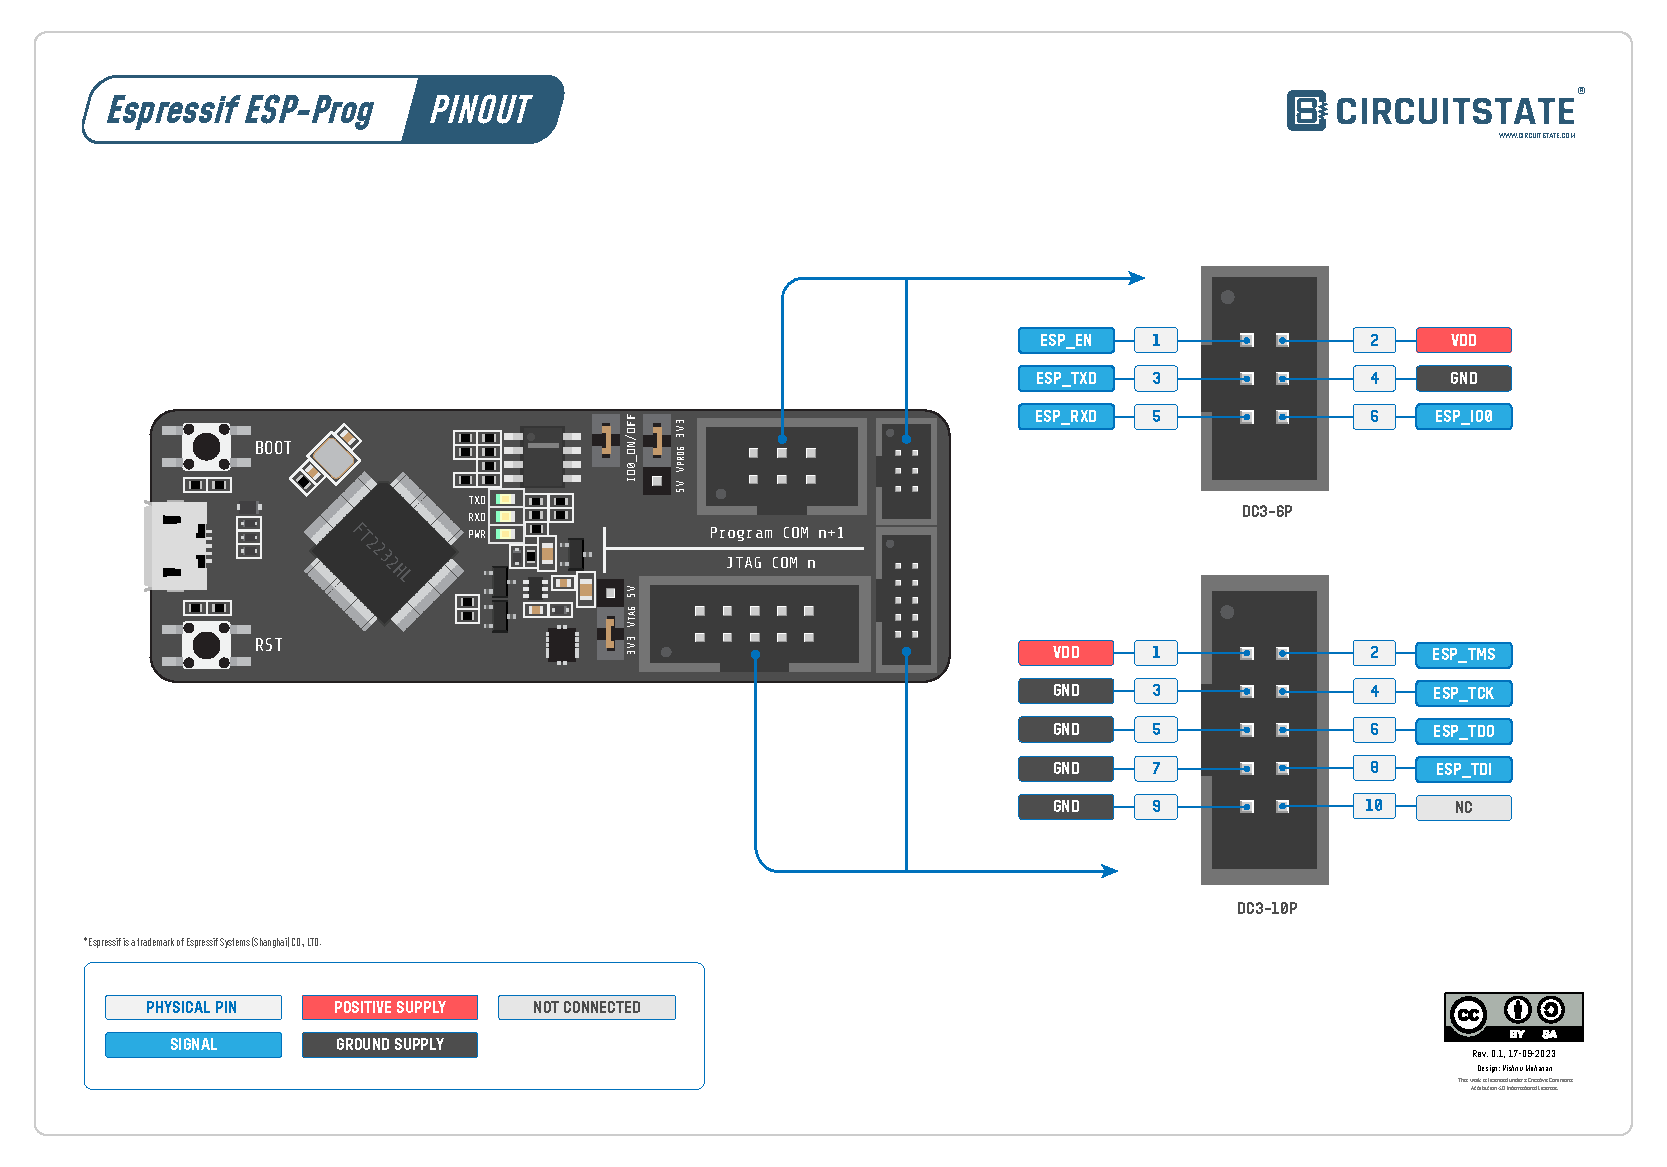
\includegraphics[width=0.8\textwidth]{figures/esp-prog-pinout.pdf}
    \caption{Diagrama del dispositivo ESP-Prog~\cite{esp-prog-pinout}.}
    \label{fig:esp-prog-pinout}
\end{figure}

Para poder utilizarlo correctamente, se deberá llevar a cabo la siguiente conexión~\cite{esp-prog-conn}:

\begin{itemize}
    \item Pin 1 ($V_{DD}$) de DC3-10P de ESP-Prog a pin 3V3 del dispositivo ESP32.
    \item Pin 2 (ESP\_TMS) de DC3-10P de ESP-Prog al pin 14 del dispositivo ESP32.
    \item Pin 3 (GND) de DC3-10P de ESP-Prog a pin GND del dispositivo ESP32.
    \item Pin 4 (ESP\_TCK) de DC3-10P de ESP-Prog al pin 13 del dispositivo ESP32.
    \item Pin 6 (ESP\_TD0) de DC3-10P de ESP-Prog al pin 15 del dispositivo ESP32.
    \item Pin 8 (ESP\_TD1) de DC3-10P de ESP-Prog al pin 12 del dispositivo ESP32.
    \item Pin 1 (ESP\_EN) de DC3-6P de ESP-Prog a pin EN del dispositivo ESP32.
    \item Pin 3 (ESP\_TXD) de DC3-6P de ESP-Prog a pin TX del dispositivo ESP32.
    \item Pin 5 (ESP\_RXD) de DC3-6P de ESP-Prog a pin RX del dispositivo ESP32.
    \item Pin 6 (ESP\_IO0) de DC3-6P de ESP-Prog al pin 0 del dispositivo ESP32.
\end{itemize}

%TODO: indicar modo de uso (comandos o cualquier mierda)


\subsection{Dilithium}\label{subsec:dilithium}

En primer lugar, se debe obtener el código de referencia de este algoritmo sobre el cual trabajar a continuación.
Este código se ha obtenido desde el repositorio oficial de CRYSTALS-Dilithium~\cite{github-dilithium}.
Dentro de este repositorio, se ha utilizado la implementación de referencia \texttt{ref}, ya que la restante, \texttt{avx2}, se encuentra optimizada para procesadores Intel con arquitectura x86.

Una vez se ha seleccionado el código a utilizar, se debe crear un proyecto que lo incluya.
Para ello, se ha creado un nuevo proyecto utilizando la extensión de Espressif en VSCode.
Los ficheros de este repositorio se han organizado tal y como se puede apreciar en la Figura~\ref{tree:dilithium}.

\begin{figure}[H]
\centering
\framebox[\textwidth]{%
\begin{minipage}{10cm}
\dirtree{%
.1 Dilithium.
.2 CMakeLists.txt.
.2 main.
.3 CMakeLists.txt.
.3 main.c.
.3 src.
.4 aes256ctr.c.
.4 fips202.c.
.4 ntt.c.
.4 packing.c.
.4 poly.c.
.4 polyvec.c.
.4 randombytes.c.
.4 reduce.c.
.4 rounding.c.
.4 sign.c.
.4 symmetric-aes.c.
.4 symmetric-shake.c.
.3 include.
.4 aes256ctr.h.
.4 api.h.
.4 config.h.
.4 fips202.h.
.4 main.h.
.4 ntt.h.
.4 packing.h.
.4 params.h.
.4 poly.h.
.4 polyvec.h.
.4 randombytes.h.
.4 reduce.h.
.4 rounding.h.
.4 sign.h.
.4 symmetric.h.
}
\end{minipage}
}
\caption{Árbol de ficheros del proyecto Dilithium.}
\label{tree:dilithium}
\end{figure}

\subsubsection{Ficheros CMake}\label{subsubsec:dilithium-cmake}

En este árbol, el archivo con ruta \texttt{Dilithium/CMakeLists.txt} únicamente especifica la versión mínima del módulo CMake para evitar posibles incompatibilidades, la inclusión del archivo \texttt{project.cmake} y la definición del nombre del proyecto.
Todo esto se refleja en el Código~\ref{lst:dilithium-cmake}.
El contenido de este fichero se ha creado teniendo en cuenta los ficheros análogos del resto de proyectos que da ESP-IDF como ejemplo.

\begin{lstlisting}[label={lst:dilithium-cmake},style=Bashnice,firstnumber=1,caption={Archivo \texttt{Dilithium/CMakeLists.txt}.}]
cmake_minimum_required(VERSION 3.16)

include($ENV{IDF_PATH}/tools/cmake/project.cmake)
project(Dilithium)
\end{lstlisting}

Dentro del directorio \texttt{main}, se han creado dos subdirectorios: \texttt{src} y \texttt{include}.
En el primero de ellos, se incluyen todos los archivos de código fuente de los que hace uso el algoritmo mientras que en el segundo de ellos se incluyen todas las librerías necesarias para su correcto funcionamiento.

Es necesario incluir, dentro del diretorio \texttt{main}, otro archivo \texttt{CMakeLists.txt} en el cual se especifiquen los archivos a incluir en la compilación del \textit{software}.
Por ello, se han incluido todos los archivos del directorio \texttt{src} como archivos fuente y el directorio \texttt{include} como directorio de librerías, tal y como se muestra en el Código~\ref{lst:dilithium-main-cmake}.

\begin{lstlisting}[label={lst:dilithium-main-cmake},style=Bashnice,firstnumber=1,caption={Archivo \texttt{Dilithium/main/CMakeLists.txt}.}]
idf_component_register(SRCS "main.c" "./src/sign.c" "./src/packing.c" "./src/polyvec.c" "./src/poly.c" "./src/ntt.c" "./src/reduce.c" "./src/rounding.c" "./src/symmetric-shake.c" "./src/symmetric-aes.c" "./src/fips202.c" "./src/aes256ctr.c" "./src/randombytes.c"
                    INCLUDE_DIRS "include")
\end{lstlisting}

\subsubsection{Generación de números aleatorios}\label{subsubsec:dilithium-random}

Un aspecto esencial consiste en la generación de número aleatorios.
Para ello, se dispone del archivo \texttt{Dilithium/main/src/randombytes.c}.
En él, se incluye la definición de la función \texttt{randombytes} (utilizada para la generación de números aleatorios de una determinada longitud) tanto para un dispositivo utilizando el sistema operativo Windows o uno basado en Linux, como se puede apreciar en el Código~\ref{lst:dilithium-randombytes}.
Inicialmente, se incluye la versión del sistema Linux ya que la compilación se lleva a cabo en un dispositivo con el sistema operativo Ubuntu 220.4 LTS.

\begin{lstlisting}[label={lst:dilithium-randombytes},style=Cnice,firstnumber=1,caption={Archivo \texttt{Dilithium/main/src/randombytes.c}.}]
#ifdef _WIN32
void randombytes(uint8_t *out, size_t outlen) {
  HCRYPTPROV ctx;
  size_t len;

  if(!CryptAcquireContext(&ctx, NULL, NULL, PROV_RSA_FULL, CRYPT_VERIFYCONTEXT))
    abort();

  while(outlen > 0) {
    len = (outlen > 1048576) ? 1048576 : outlen;
    if(!CryptGenRandom(ctx, len, (BYTE *)out))
      abort();

    out += len;
    outlen -= len;
  }

  if(!CryptReleaseContext(ctx, 0))
    abort();
}
#elif defined(__linux__) && defined(SYS_getrandom)
void randombytes(uint8_t *out, size_t outlen) {
  ssize_t ret;

  while(outlen > 0) {
    ret = syscall(SYS_getrandom, out, outlen, 0);
    if(ret == -1 && errno == EINTR)
      continue;
    else if(ret == -1)
      abort();

    out += ret;
    outlen -= ret;
  }
}
\end{lstlisting}

Teniendo esto en cuenta, es necesaria la inclusión de una opción indicada para el dispositivo ESP32 y la compilación de esta en vez de la diseñada para los sistemas basados en Linux.
Para ello, se ha añadido la definición especificada en el Código~\ref{lst:dilithium-randombytes-esp32}.
En ella, se utiliza la función \texttt{esp\_fill\_random}~\cite{esp32-random} la cual genera un número aleatorio de longitud \texttt{outlen} y lo almacena en \texttt{out}.
Estos números aleatorios son generados mediante una fuente \textit{hardware}.

\begin{lstlisting}[label={lst:dilithium-randombytes-esp32},style=Cnice,firstnumber=1,caption={Generación de números aleatorios para ESP32.}]
#elif defined(ESP32)
#include "esp_random.h"

void randombytes(uint8_t *out, size_t outlen) {
  esp_fill_random(out, outlen);
}
#endif
\end{lstlisting}


\subsubsection{Fichero de comprobación}\label{subsubsec:dilithium-main}

Una vez se han incluido y referenciado todos los archivos, es necesario crear una prueba que nos permita comprobar la ejecución del algoritmo.
Para ello, se ha creado el archivo \texttt{main.c}, el cual está formado por el contenido mostrado en el Código~\ref{lst:dilithium-main}.
En este fichero, se ejecuta la generación de claves (\texttt{crypto\_sign\_keypair}) y se comprueba si ha existido algún error en la generación.
Una vez se han obtenido las claves pública (\texttt{pk}) y privada (\texttt{sk}), se lleva a cabo la firma de un mensaje previamente especificado (\texttt{m} con longitud \texttt{mlen}) con la función \texttt{crypto\_sign}.
El resultado de esta operación se almacena en la variable \texttt{sm} con longitud \texttt{smlen} y se comprueba si esta firma se ha relizado correctamente.
Finalmente, se lleva a cabo la función de comprobación de firma con la función \texttt{crypto\_sign\_open}.
Una vez realizada, se almacena el mensaje recuperado en la variable \texttt{m1} con longitud \texttt{mlen1}.
Para comprobar la integridad de este mensaje, se compara la longitud y contenido del mensaje recuperado y del mensaje inicial.
Si estos dos parámetros coinciden, la prueba ha sido exitosa.

\begin{lstlisting}[label={lst:dilithium-main},style=Cnice,firstnumber=1,caption={Archivo \texttt{Dilithium/main/main.c}.}]
#include <stdio.h>
#include <string.h>

#include "api.h"
#include "main.h"
    
void app_main(void)
{
    printf("Inicio con la opción %d\n\r", DILITHIUM_MODE);

    //Generación de claves
    uint8_t *pk = (uint8_t*) malloc(CRYPTO_PUBLICKEYBYTES * sizeof(uint8_t));
    uint8_t *sk = (uint8_t*) malloc(CRYPTO_SECRETKEYBYTES * sizeof(uint8_t));
    if (crypto_sign_keypair(pk, sk) != 0) {
        printf("Generacion de claves fallida\n\r");
    } else {
        printf("Generacion de claves exitosa (%d bytes de clave publica y %d bytes de clave privada)\n\r", CRYPTO_PUBLICKEYBYTES, CRYPTO_SECRETKEYBYTES);
    }

    //Firma de mensaje
    uint8_t m[] = "Esto es una prueba de la firma de mensajes utilizando Dilithium.";
    size_t mlen = sizeof(m), smlen;
    uint8_t *sm = (uint8_t *)calloc(mlen+CRYPTO_BYTES, sizeof(uint8_t));
    if (crypto_sign(sm, &smlen, m, mlen, sk) != 0) {
        printf("Firma de mensaje fallida\n\r");
    } else {
        printf("Firma del mensaje exitosa (%d bytes de firma)\n\r", mlen+CRYPTO_BYTES);
    }

    //Comprobación de la firma
    size_t mlen1;
    uint8_t *m1 = (uint8_t *)calloc(mlen+CRYPTO_BYTES, sizeof(uint8_t));
    if (crypto_sign_open(m1, &mlen1, sm, smlen, pk) != 0) {
        printf("Comprobacion de la firma fallida\n\r");
    } else {
        if (mlen != mlen1) {
            printf("Longitud del mensaje original distinta a la longitud del mensaje recuperado\n\r");
        } else if (memcmp(m, m1, mlen)) {
            printf("Contenido del mensaje original distinto al contenido del mensaje recuperado\n\r");
        } else {
            printf("Comprobacion de la firma del mensaje exitosa (%d bytes de mensaje)\n\r", mlen1);
        }
    }

    //Liberación de la memoria reservada
    free(pk);
    free(sk);
    free(m1);
    free(sm);
}
\end{lstlisting}

Como se puede observar en el Código~\ref{lst:dilithium-main}, se hace referencia al fichero \texttt{main.h}.
Este fichero únicamente contiene la especificación de la versión del algoritmo mediante la definición de \texttt{DILITHIUM\_MODE}, como se muestra en el Código~\ref{lst:dilithium-mainh}.
También, se elimina la definición previa de \texttt{\_\_linux\_\_} y la definición de \texttt{ESP32}, cuyo motivo se trata en la apartado~\ref{subsubsec:dilithium-random}.

\begin{lstlisting}[label={lst:dilithium-mainh},style=Cnice,firstnumber=1,caption={Archivo \texttt{Dilithium/main/include/main.h}.}]
#ifndef MAIN_H
#define MAIN_H

//Necesario para generación de números aleatorios
#ifdef __linux__
    #undef __linux__
#endif
#ifndef ESP32
    #define ESP32
#endif

#ifndef DILITHIUM_MODE
    #define DILITHIUM_MODE 3	/*{2,3,5}*/
#endif
#endif
\end{lstlisting}


\subsubsection{Uso de memoria dinámica}\label{subsubsec:dilithium-dynamic}

Una vez realizados todos los pasos anteriores, el siguiente paso consiste en la ejecución de la comprobación del algoritmo.
Al ejecutarlo, se comprueba que la ejecución se bloquea en la generación de claves sin mostrar ningún código de error.
LLevando a cabo distinta comprobaciones, se encontró que le error sucedía en la función \texttt{KeccakF1600\_StatePermute} dentro del archivo \texttt{fips202.c}, aunque no se puedo concretar la instrucción exacta en la que sucedía el error.
Por ello, se ha requerido utilizar el depurador ESP-Prog.
A través del depurador, se ha concluido que el error surge del error que se aprecia en la Captura~\ref{}.

%TODO: captura error depurador

Según se ha encontrado en distintas entradas del foro oficial de ESP32~\cite{esp32-forum1}~\cite{esp32-forum2}~\cite{esp32-forum2}, este error se debe, sin duda, a un problema en la memoria del dispositivo.
En una de estas entradas, se sugiere la posibilidad de un \textit{overflow} del \textit{stack} sea el causante de este problema.
Este problema surge del hecho de que, antes de ejecutar el programa de prueba, se realiza una reserva de memoria automáticamente y la cantidad de memoria reservada es inferior a la necesitada posteriormente.
Por ello, se debe hacer uso de la memoria \textit{heap} en vez de la memoria \textit{stack}.
Con esta idea en mente, se ha llevado a cabo la modificación de la implementación inicial para hacer uso de memoria dinámica y evitar el \textit{overflow} del \textit{stack} al requerir un tamaño mucho menor de esta memoria.
De esta forma, la cantidad de memoria reservada inicialmente no será sobrepasada por la cantidad de memoria en \textit{stack} requerida.

Las primeras variables en ser modificadas han sido las incluidas en el archivo \texttt{main.c}, las cuales representan las claves pública, privada y firma del mensaje y, por ende, una gran cantidad de datos (1312, 2528 y 2420 bytes respectivamente en Dilithium2).
Esto se puede apreciar en el Código~\ref{lst:dilithium-main}.

\begin{lstlisting}[label={lst:dilithium-key-dyn},style=Cnice,firstnumber=1,caption={Modificación de la función \texttt{crypto\_sign\_keypair} en el archivo \texttt{Dilithium/main/src/sign.c}.}]
int crypto_sign_keypair(uint8_t *pk, uint8_t *sk) {
  uint8_t seedbuf[2*SEEDBYTES + CRHBYTES];
  uint8_t tr[SEEDBYTES];
  const uint8_t *rho, *rhoprime, *key;
  polyvecl *mat = (polyvecl*) malloc(K * sizeof(polyvecl));
  polyvecl *s1 = (polyvecl*) malloc( sizeof(polyvecl));
  polyvecl *s1hat = (polyvecl*) malloc( sizeof(polyvecl));
  polyveck *s2 = (polyveck*) malloc( sizeof(polyveck));
  polyveck *t1 = (polyveck*) malloc( sizeof(polyveck));
  polyveck *t0 = (polyveck*) malloc( sizeof(polyveck));

  ...

  free(mat);
  free(s1);
  free(s1hat);
  free(s2);
  free(t1);
  free(t0);

  return 0;
}
\end{lstlisting}

En la modificación mostrada en el Código~\ref{lst:dilithium-key-dyn}, se han priorizado las variables de mayor tamaño, como en este caso todas las variables del tipo \texttt{polyvecl}, ya que esta estructura consta de un tamaño de 4 kB en Dilithium2, 6 kB en Dilithium3 y 8 kB en Dilithium5.
También, las variables de tipo \texttt{polyveck} ya que esta estructura requiere de un tamaño de 4 kB en Dilithium2, 5 kB en Dilithium3 y 7 kB en Dilithium5.

\begin{lstlisting}[label={lst:dilithium-sign-dyn},style=Cnice,firstnumber=1,caption={Modificación de la función \texttt{crypto\_sign\_signature} en el archivo \texttt{Dilithium/main/src/sign.c}.}]
int crypto_sign_signature(uint8_t *sig, size_t *siglen, const uint8_t *m, size_t mlen, const uint8_t *sk)
{
  unsigned int n;
  uint8_t seedbuf[3*SEEDBYTES + 2*CRHBYTES];
  uint8_t *rho, *tr, *key, *mu, *rhoprime;
  uint16_t nonce = 0;
  polyvecl *mat = (polyvecl*) malloc(K * sizeof(polyvecl));
  polyvecl *s1 = (polyvecl*) malloc(sizeof(polyvecl));
  polyvecl *y  = (polyvecl*) malloc(sizeof(polyvecl));
  polyvecl *z  = (polyvecl*) malloc(sizeof(polyvecl));

  polyveck *t0 = (polyveck*) malloc(sizeof(polyveck));
  polyveck *s2 = (polyveck*) malloc(sizeof(polyveck));
  polyveck *w1 = (polyveck*) malloc(sizeof(polyveck));
  polyveck *w0 = (polyveck*) malloc(sizeof(polyveck));
  polyveck *h  = (polyveck*) malloc(sizeof(polyveck));
  poly *cp = (poly*) malloc(sizeof(poly));
  keccak_state *state = (keccak_state*) malloc(sizeof(keccak_state));

  ...

  free(mat);
  free(s1);
  free(y);
  free(z);
  free(t0);
  free(s2);
  free(w1);
  free(w0);
  free(h);
  free(cp);
  free(state);

  return 0;
}
\end{lstlisting}

A continuación, se modificó la función \texttt{crypto\_sign\_signature} mediante el Código~\ref{lst:dilithium-sign-dyn}.
En este caso, se han alterado las variables de tipo \texttt{polyveck} y \texttt{polyvecl} por el mismo motivo explicado anteriormente.
Además, se han adaptado las variables \texttt{cp} y \texttt{state} a pesar de no requerir una gran cantidad de memoria.

\begin{lstlisting}[label={lst:dilithium-ver-dyn},style=Cnice,firstnumber=1,caption={Modificación de la función \texttt{crypto\_sign\_verify} en el archivo \texttt{Dilithium/main/src/sign.c}.}]
int crypto_sign_verify(const uint8_t *sig,
                       size_t siglen,
                       const uint8_t *m,
                       size_t mlen,
                       const uint8_t *pk)
{
  unsigned int i;
  uint8_t *buf = (uint8_t *)malloc((K*POLYW1_PACKEDBYTES) * sizeof(uint8_t));
  uint8_t rho[SEEDBYTES];
  uint8_t mu[CRHBYTES];
  uint8_t c[SEEDBYTES];
  uint8_t c2[SEEDBYTES];
  poly *cp = (poly*) malloc(sizeof(poly));
  polyvecl *mat = (polyvecl*) malloc(K * sizeof(polyvecl));
  polyvecl *z   = (polyvecl*) malloc(sizeof(polyvecl));;

  polyveck *t1 = (polyveck*) malloc(sizeof(polyveck));
  polyveck *w1 = (polyveck*) malloc(sizeof(polyveck));
  polyveck *h = (polyveck*) malloc(sizeof(polyveck));
  keccak_state *state = (keccak_state*) malloc(sizeof(keccak_state));

  ...

  free(buf);
  free(cp);
  free(mat);
  free(z);
  free(t1);
  free(w1);
  free(h);
  free(state);

  return 0;
}
\end{lstlisting}

Por último, se ha modificado la función \texttt{crypto\_sign\_verify} tal y como se muestra en el Código~\ref{lst:dilithium-ver-dyn}.
Para esta modificación se ha seguido la pauta anteriormente especificada, en la cual se modifican las variables de tipo \texttt{polyveck} \texttt{polyvecl}.
Además, en este caso, se ha modificado la variable \texttt{buf} ya que esta necesitaría 768 bytes en Dilithium2 y Dilithium3 y 1 kB en el caso de Dilithium5.

Una vez realizadas todas estas modificaciones, se han adaptado las llamadas a las funciones que componen \texttt{crypto\_sign\_keypair}, \texttt{crypto\_sign\_signature} y \texttt{crypto\_sign\_verify} de forma que se utilicen correctamente los punteros creados en lugar de las variables utilizadas anteriormente.


\subsubsection{Comprobación del algoritmo}\label{subsubsec:dilithium-compro}

Tras completar todos los pasos indicados previamente, se lleva a cabo la ejecución del algoritmo.
Esta ejecución se lleva a cabo mediante el programa mostrado en el Código~\ref{lst:dilithium-main}.
El resultado de esta ejecución se muestra en la Captura~\ref{}.

%TODO: ejecución Dilithium



\subsection{Kyber}\label{subsec:kyber}

\begin{figure}[H]
\centering
\framebox[\textwidth]{%
\begin{minipage}{10cm}
\dirtree{%
.1 Kyber.
.2 CMakeLists.txt.
.2 main.
.3 CMakeLists.txt.
.3 main.c.
.3 src.
.4 aes256ctr.c.
.4 cbd.c.
.4 cpucycles.c.
.4 fips202.c.
.4 indcpa.c.
.4 kem.c.
.4 kex.c.
.4 ntt.c.
.4 poly.c.
.4 polyvec.c.
.4 randombytes.c.
.4 reduce.c.
.4 rng.c.
.4 sha256.c.
.4 sha512.c.
.4 speed\_print.c.
.4 symmetric-aes.c.
.4 symmetric-shake.c.
.4 verify.c.
.3 include.
.4 aes256ctr.h.
.4 api.h.
.4 cbd.h.
.4 cpucycles.h.
.4 fips202.h.
.4 indcpa.h.
.4 kem.h.
.4 kex.h.
.4 main.h.
.4 ntt.h.
.4 params.h.
.4 poly.h.
.4 polyvec.h.
.4 randombytes.h.
.4 reduce.h.
.4 rng.h.
.4 sha2.h.
.4 speed\_print.h.
.4 symmetric.h.
.4 verify.h.
}
\end{minipage}
}
\caption{Árbol de ficheros del proyecto Kyber.}
\label{tree:kyber}
\end{figure}

Al igual que para el caso de Dilithium~\ref{subsec:dilithium}, el primer paso consiste en seleccionar la implementación a tratar.
Para ello, se ha utilizado el repositorio oficial de CRYSTALS-Kyber~\cite{github-kyber}.
Dentro de este código, existe tanto una implementación estándar dentro del directorio \texttt{ref} y otra optimizada para procesadores Intel x86 bajo el nombre \texttt{avx2}.

Repitiendo los pasos descritos para Dilithium, se ha procedido a crear un proyecto mediante la extensión de Espressif en VSCode.
El árbol de ficheros utilizado es el mostrado en la Figura~\ref{tree:kyber}.

\subsubsection{Ficheros CMake}\label{subsubsec:kyber-cmake}

Dentro de este árbol, el archivo \texttt{Kyber/CMakeLists.txt} indica la versión mínima aceptada del módulo CMake para evitar posibles incompatibilidades, el uso del archivo \texttt{project.cmake} y el nombre del proyecto.
Todo esto se refleja en el Código~\ref{lst:kyber-cmake}.
El contenido de este fichero se ha creado teniendo en cuenta los ficheros análogos del resto de proyectos que da ESP-IDF como ejemplo.

\begin{lstlisting}[label={lst:kyber-cmake},style=Bashnice,firstnumber=1,caption={Archivo \texttt{Kyber/CMakeLists.txt}.}]
cmake_minimum_required(VERSION 3.16)

include($ENV{IDF_PATH}/tools/cmake/project.cmake)
project(Kyber)
\end{lstlisting}

Dentro del directorio \texttt{main}, se han creado dos subdirectorios: \texttt{src} y \texttt{include}.
En el primero de ellos, se incluyen todos los archivos de código fuente de los que hace uso el algoritmo mientras que en el segundo de ellos se incluyen todas las librerías necesarias para su correcto funcionamiento.

Es necesario incluir, dentro del diretorio \texttt{main}, otro archivo \texttt{CMakeLists.txt} en el cual se especifiquen los archivos a incluir en la compilación del \textit{software}.
Por ello, se han incluido todos los archivos del directorio \texttt{src} como archivos fuente y el directorio \texttt{include} como directorio de librerías, tal y como se muestra en el Código~\ref{lst:kyber-main-cmake}.

\begin{lstlisting}[label={lst:kyber-main-cmake},style=Bashnice,firstnumber=1,caption={Archivo \texttt{Kyber/main/CMakeLists.txt}.}]
idf_component_register(SRCS "main.c" "src/kex.c" "src/kem.c" "src/indcpa.c" "src/polyvec.c" "src/poly.c" "src/cbd.c" "src/ntt.c" "src/reduce.c" "src/verify.c" "src/symmetric-shake.c" "src/symmetric-aes.c" "src/fips202.c" "src/randombytes.c"
    INCLUDE_DIRS "include")
\end{lstlisting}

\subsubsection{Generación de números aleatorios}\label{subsubsec:kyber-random}

Teniendo en cuenta que el dispositivo utilizado es el mismo que para el algoritmo Dilithium, la generación de números aleatorios se realiza de la misma manera que la mostrada en el Código~\ref{lst:dilithium-randombytes-esp32}.
Además, debido a que tanto Dilithium como Kyber comparten creadores, la generación de números aleatorios es idéntica, por lo que el archivo de generación de números aleatorios \texttt{Kyber/main/src/randombytes.c} es el mismo y, por ende, la forma en la que incluir la versión para el ESP32.

\subsubsection{Fichero de comprobación}\label{subsubsec:kyber-main}

Una vez se han incluido y referenciado todos los archivos, es necesario crear una prueba que nos permita comprobar la ejecución del algoritmo.
Para ello, se ha creado el archivo \texttt{main.c}, el cual está formado por el contenido mostrado en el Código~\ref{lst:kyber-main}.
En primer lugar, se llama a la función \texttt{crypto\_kem\_keypair}, encargada de generar las claves tanto pública como privada a utilizar.
La clave pública se almacenará en la variable \texttt{pk} mientras que la clave privada estará representada por \texttt{sk}.
Si esta generación fuese errónea, la ejecución finalizaría.
En caso contrario, se llevaría a cabo la generación del secreto compartido (\texttt{ss\_pub}) y del cifrado (\texttt{ct}) haciendo uso de la clave pública mediante la función \texttt{crypto\_kem\_enc}.
A continuación, se utiliza la función \texttt{crypto\_kem\_dec}, a la cual se entrega el cifrado \texttt{ct} generado por la función anterior y la clave privada y devuelve el secreto compartido \texttt{ss\_priv}, el cual, si la ejecución ha sido correcta, debería coincidir con el secreto generado anteriormente \texttt{ss\_pub}.
Para finalizar, se lleva a cabo esta verificación y se libera la memoria correspondiente a las variables creadas al inicio del programa.

\begin{lstlisting}[label={lst:kyber-main},style=Cnice,firstnumber=1,caption={Archivo \texttt{Kyber/main/main.c}.}]
#include <stdio.h>
#include <stdlib.h>
#include <string.h>
#include <ctype.h>

#include "main.h"
#include "kem.h"
#include "api.h"

#include "randombytes.h"

void app_main (void)
{
    printf("Inicio con la opción %d\n\r", KYBER_K);

    //Generación de claves
    unsigned char *pk = (unsigned char*) malloc(CRYPTO_PUBLICKEYBYTES * sizeof(unsigned char));
    unsigned char *sk = (unsigned char*) malloc(CRYPTO_SECRETKEYBYTES * sizeof(unsigned char));
    if (crypto_kem_keypair(pk, sk) != 0) {
        printf("Generacion de claves fallida\n\r");
        return;
    } else {
        printf("Generacion de claves exitosa (%d bytes de clave publica y %d bytes de clave privada)\n\r", CRYPTO_PUBLICKEYBYTES, CRYPTO_SECRETKEYBYTES);
    }

    //Generación de texto cifrado y secreto compartido
    unsigned char *ct = (unsigned char*) malloc(CRYPTO_CIPHERTEXTBYTES * sizeof(unsigned char));
    unsigned char *ss_pub = (unsigned char*) malloc(CRYPTO_BYTES * sizeof(unsigned char));
    if (crypto_kem_enc(ct, ss_pub, pk) != 0) {
        printf("Generacion de texto cifrado y secreto compartido fallida\n\r");
        return;
    } else {
        printf("Generacion de texto cifrado y secreto compartido exitosa (%d bytes de texto cifrado y %d bytes de secreto compartido)\n\r", CRYPTO_CIPHERTEXTBYTES, CRYPTO_BYTES);
    }

    //Generación de secreto compartido
    unsigned char *ss_priv = (unsigned char*) malloc(CRYPTO_BYTES * sizeof(unsigned char));
    if (crypto_kem_dec(ss_priv, ct, sk) != 0) {
        printf("Generacion de secreto compartido fallida\n\r");
        return;
    } else {
        printf("Generacion de secreto compartido exitosa (%d bytes de secreto compartido)\n\r", CRYPTO_BYTES);
    }

    //Comprobación de resultados
    if (memcmp(ss_pub, ss_priv, (unsigned int) CRYPTO_BYTES) ) {
        printf("Comprobación fallida\n\r");
    } else{
        printf("¡Comprobación superada!\n\r");
    }

    //Liberación de la memoria reservada
    free(pk);
    free(sk);
    free(ct);
    free(ss_pub);
    free(ss_priv);
}
\end{lstlisting}

Como se puede observar en el Código~\ref{lst:kyber-main}, se hace referencia al fichero \texttt{main.h}.
Este fichero únicamente contiene la especificación de la versión del algoritmo mediante la definición de \texttt{KYBER\_K}, como se muestra en el Código~\ref{lst:kyber-mainh}.
También, se elimina la definición previa de \texttt{\_\_linux\_\_} y la definición de \texttt{ESP32}, cuyo motivo se trata en la apartado~\ref{subsubsec:dilithium-random}.

\begin{lstlisting}[label={lst:kyber-mainh},style=Cnice,firstnumber=1,caption={Archivo \texttt{Kyber/main/include/main.h}.}]
#ifndef MAIN_H
#define MAIN_H

//Necesario para generación de números aleatorios
#ifdef __linux__
    #undef __linux__
#endif
#ifndef ESP32
    #define ESP32
#endif

#ifndef KYBER_K
    #define KYBER_K 3
#endif
#endif
\end{lstlisting}


\subsubsection{Uso de memoria dinámica}\label{subsubsec:kyber-dynamic}

De la misma manera que Dilithium suponía un \textit{overflow} en el \textit{stack} reservado, Kyber también, como se puede comprobar en la Figura~\ref{}.

%TODO: captura error depurador

Por ello, se han seguido los mismos pasos y se ha hecho uso de la \textit{heap} cambiando las variables estáticas que más memoria requerían a ser variables dinámicas.
El archivo en ser modificado ha sido el archivo \texttt{Kyber/main/src/indcpa.c}.
En él, se ha cambiado la función \texttt{indcpa\_keypair} tal y como se indica en el Código~\ref{lst:kyber-key-dyn}.

\begin{lstlisting}[label={lst:kyber-key-dyn},style=Cnice,firstnumber=1,caption={Modificación de la función \texttt{indcpa\_keypair} en el archivo \texttt{Kyber/main/src/indcpa.c}.}]
void indcpa_keypair(uint8_t pk[KYBER_INDCPA_PUBLICKEYBYTES], uint8_t sk[KYBER_INDCPA_SECRETKEYBYTES])
{
  unsigned int i;
  uint8_t *buf = (uint8_t*) malloc(2*KYBER_SYMBYTES * sizeof(uint8_t));
  const uint8_t *publicseed = buf;
  const uint8_t *noiseseed = buf+KYBER_SYMBYTES;
  uint8_t nonce = 0;

  polyvec *a = (polyvec*) malloc(KYBER_K * sizeof(polyvec));
  polyvec *e = (polyvec*) malloc(sizeof(polyvec));
  polyvec *pkpv = (polyvec*) malloc(sizeof(polyvec));
  polyvec *skpv = (polyvec*) malloc(sizeof(polyvec));

  ...

  free(buf);
  free(a);
  free(e);
  free(skpv);
  free(pkpv);
}
\end{lstlisting}

En este caso, las variables de tipo \texttt{polyvec} ocupan 1 kB en le caso de Kyber2, 1.5 kB en el caso de Kyber3 y 2 kB en el caso de Kyber4.
La variable \texttt{a} ocupa un total de 2 kB para Kyber2, 3.5 kB para Kyber3 y 8 kB para Kyber4.
Por ello, todas estas variables han sido modificadas para hacer uso de memoria dinámica en vez de memoria estática, siguiendo el próposito indicado en el apartado~\ref{subsubsec:dilithium-dynamic}.

\begin{lstlisting}[label={lst:kyber-enc-dyn},style=Cnice,firstnumber=1,caption={Modificación de la función \texttt{indcpa\_enc} en el archivo \texttt{Kyber/main/src/indcpa.c}.}]
void indcpa_enc(uint8_t c[KYBER_INDCPA_BYTES], const uint8_t m[KYBER_INDCPA_MSGBYTES], const uint8_t pk[KYBER_INDCPA_PUBLICKEYBYTES], const uint8_t coins[KYBER_SYMBYTES])
{
    unsigned int i;
    uint8_t *seed = (uint8_t*) malloc(KYBER_SYMBYTES * sizeof(uint8_t));
    uint8_t nonce = 0;

    polyvec *sp   = (polyvec*) malloc(sizeof(polyvec));
    polyvec *pkpv = (polyvec*) malloc(sizeof(polyvec));
    polyvec *ep   = (polyvec*) malloc(sizeof(polyvec));
    polyvec *at   = (polyvec*) malloc(KYBER_K * sizeof(polyvec));
    polyvec *b    = (polyvec*) malloc(sizeof(polyvec));

    poly *v   = (poly*) malloc(sizeof(poly));
    poly *k   = (poly*) malloc(sizeof(poly));
    poly *epp = (poly*) malloc(sizeof(poly));

    ...

    free(seed);
    free(sp);
    free(pkpv);
    free(ep);
    free(at);
    free(b);
    free(v);
    free(k);
    free(epp);
}
\end{lstlisting}

En el Código~\ref{lst:kyber-enc-dyn} se observa la modificación realizada en la función encargada de generar el secreto compartido y el cifrado.
Para ello, se han modificado las variables del tipo \texttt{polyvec} y del tipo \texttt{poly}, aunque estas últimas requieren una cantidad de memoria mucho menor.

\begin{lstlisting}[label={lst:kyber-dec-dyn},style=Cnice,firstnumber=1,caption={Modificación de la función \texttt{indcpa\_dec} en el archivo \texttt{Kyber/main/src/indcpa.c}.}]
void indcpa_dec(uint8_t m[KYBER_INDCPA_MSGBYTES], const uint8_t c[KYBER_INDCPA_BYTES], const uint8_t sk[KYBER_INDCPA_SECRETKEYBYTES])
{
  polyvec *b    = (polyvec*) malloc(sizeof(polyvec));
  polyvec *skpv = (polyvec*) malloc(sizeof(polyvec));

  poly *v  = (poly*) malloc(sizeof(poly));
  poly *mp = (poly*) malloc(sizeof(poly));

  ...

  free(b);
  free(skpv);
  free(v);
  free(mp);
}
\end{lstlisting}

La última función modificada ha sido la encargad de obtener el secreto compartido apartir del cifrado y la clave privada, \texttt{indcpa\_dec}.
Siguiendo los cambios realizados con anterioridad, se han modificado las variables del tipo \texttt{polyvec} y \texttt{poly}.

\subsubsection{Comprobación del algoritmo}\label{subsubsec:kyber-compro}

Para finalizar con este algoritmo, se ha llevado a cabo la comprobación de su funcionamiento utilizando el Código~\ref{lst:kyber-main}.
El resultado de esta ejecución se muestra en la Captura~\ref{}.

%TODO: ejecución Kyber




\section{RP2040}\label{sec:rp2040}

El siguiente dispositivo a utilizar es el Lyligo T-Display~\cite{lilygo}, el cual incluye un ESP32 y un RP2040.
Este dispositivo utiliza el conector USB-C para programar un elemento u otro, dependiendo si está conectado con una orientación u otra.

Para poder programar el RP2040 se ofrecen varias posibilidades en el repositorio de esta plataforma.
Estas posibilidades son: Arduino, Mycropython y Pico SDK.
Los algoritmos a implementar están desarrollados sobre C, lo cual da un mayor control sobre los recursos del dispositivo.
En cambio, Arduino está implementado en una mezcla de C y C++, por lo que puede no ser óptimo a la hora de utilizar aplicaciones exigentes en lo referente a recursos.
En este aspecto, Micropython tiene el mismo defecto.
Por otro lado, Pico SDK supone directamente una programación en C, lo cual consigue un mejor uso de los recursos disponibles.


\subsection{Pico SDK}\label{subsec:pico-sdk}

La herramienta Pico SDK~\cite{pico-sdk} está desarrollada para otorgar al usuario el mayor control posible sobre el dispositivo.
Este ejecuta un programa con la función \texttt{main} convencional y aporta varias librerías que permiten tratar con temporizadores, conexiones USB y sincronización.

Para la construcción de los projectos, esta herramienta hace uso de CMake ya que es soportado por multitud de IDEs.
Para poder utilizar esta herramienta, se deben seguir los pasos indicados en su repositorio oficial~\cite{pico-sdk-github}.
En primer lugar, se deben instalar los paquetes necesarios con el comando \texttt{sudo apt install cmake gcc-arm-none-eabi libnewlib-arm-none-eabi libstdc++-arm-none-eabi-newlib}.
A continuación, se debe clonar el repositorio de la herramienta con el comando \texttt{git clone https://github.com/raspberrypi/pico-sdk.git}.
Posteriormente, es necesario copiar el archivo \texttt{pico\_sdk\_import.cmake} en el proyecto y establecer la variable de entorno \texttt{PICO\_SDK\_PATH} con la ruta al repositorio recién clonado.
El siguiente paso consiste en crear un archivo CMakeLists.txt como el ejemplo mostrado en el Código~\ref{lst:sdk-example} y el programa que se vaya a ejecutar en el dispositivo.
Por último, se debe crear un directorio \texttt{build} mediante el comando \texttt{mkdir build \&\& cd build \&\& cmake ..} y, dentro del directorio \texttt{build}, ejecutar el comando \texttt{make hello\_world} para construir el ejecutable del programa creado.
Esto genera un archivo .elf para cargar a través de un depurador y un archivo .elf2 para cargar directamente mediante la conexión \ac{USB}.

\begin{lstlisting}[label={lst:sdk-example},style=Cnice,firstnumber=1,caption={Ejemplo de CMakeLists.txt~\cite{pico-sdk-github}.}]
cmake_minimum_required(VERSION 3.13)

# initialize the SDK based on PICO_SDK_PATH
# note: this must happen before project()
include(pico_sdk_import.cmake)

project(my_project)

# initialize the Raspberry Pi Pico SDK
pico_sdk_init()

# rest of your project
\end{lstlisting}


\subsection{HQC-128}\label{subsec:hqc}

El primer algoritmo a implementar en este dispositivo ha sido el algoritmo HQC-128.
Para comenzar, se debe obtener una implementación del mismo.
La implementación seleccionada ha sido la correspondiente al proyecto PQClean~\cite{SSR:KSSW22}.
El código correspondiente a este algoritmo se puede encontrar en su repositorio de GitHub~\cite{pqclean-github}.

Una vez extraídos los archivos correspondientes a este algoritmo, se han colocado de la forma indicada en el árbol de ficheros~\ref{tree:hqc}.

\begin{figure}[H]
\centering
\framebox[\textwidth]{%
\begin{minipage}{10cm}
\dirtree{%
.1 HQC-128.
.2 main.c.
.2 CMakeLists.txt.
.2 src.
.3 code.c.
.3 fft.c.
.3 fips202.c.
.3 gf.c.
.3 gf2x.c.
.3 hqc.c.
.3 kem.c.
.3 parsing.c.
.3 randombytes.c.
.3 reed\_muller.c.
.3 reed\_solomon.c.
.3 shake\_ds.c.
.3 shake\_prng.c.
.3 vector.c.
.2 include.
.3 api.h.
.3 code.h.
.3 fft.h.
.3 fips202.h.
.3 gf.h.
.3 gf2x.h.
.3 hqc.h.
.3 main.h.
.3 parameters.h.
.3 parsing.h.
.3 randombytes.h.
.3 reed\_muller.h.
.3 reed\_solomon.h.
.3 shake\_ds.h.
.3 shake\_prng.h.
.3 vector.h.
}
\end{minipage}
}
\caption{Árbol de ficheros del proyecto HQC-128.}
\label{tree:hqc}
\end{figure}

Este proyecto incluye, al igual que los proyectos del dispositivo ESP32, todos los ficheros de código fuente en un directorio \texttt{src} y todas librerías en un directorio \texttt{include}.
Además, dispone de un archivo CMakeLists.txt que se explica en el apartado~\ref{subsubsec:hqc-cmake} y un archivo de comprobación que se detalla en el apartado~\ref{subsubsec:hqc-main}.


\subsubsection{Fichero CMake}\label{subsubsec:hqc-cmake}

Dentro de este archivo CMakelists.txt, se puede hallar el contenido del Código~\ref{lst:hqc-make}.

\begin{lstlisting}[label={lst:hqc-make},style=Cnice,firstnumber=1,caption={Archivo \texttt{HQC-128/CMakeLists.txt}.}]
cmake_minimum_required(VERSION 3.13)

if (TARGET tinyusb_device)
    add_compile_options(-Wall -Wextra -Wpedantic -Wredundant-decls -Wcast-align -Wmissing-prototypes -DPQCLEAN_NAMESPACE=PQCLEAN_HQC128_CLEAN)

    add_executable(hqc-128)

    target_sources(hqc-128 PUBLIC
            ${CMAKE_CURRENT_LIST_DIR}/main.c
            ${CMAKE_CURRENT_LIST_DIR}/src/code.c
            ${CMAKE_CURRENT_LIST_DIR}/src/fft.c
            ${CMAKE_CURRENT_LIST_DIR}/src/gf.c
            ${CMAKE_CURRENT_LIST_DIR}/src/gf2x.c
            ${CMAKE_CURRENT_LIST_DIR}/src/hqc.c
            ${CMAKE_CURRENT_LIST_DIR}/src/kem.c
            ${CMAKE_CURRENT_LIST_DIR}/src/parsing.c
            ${CMAKE_CURRENT_LIST_DIR}/src/reed_muller.c
            ${CMAKE_CURRENT_LIST_DIR}/src/reed_solomon.c
            ${CMAKE_CURRENT_LIST_DIR}/src/shake_ds.c
            ${CMAKE_CURRENT_LIST_DIR}/src/shake_prng.c
            ${CMAKE_CURRENT_LIST_DIR}/src/vector.c
            ${CMAKE_CURRENT_LIST_DIR}/src/randombytes.c
            ${CMAKE_CURRENT_LIST_DIR}/src/fips202.c
            )
    
    target_include_directories(hqc-128 PUBLIC
                    ${CMAKE_CURRENT_LIST_DIR}/include)

    # pull in common dependencies
    target_link_libraries(hqc-128 pico_stdlib pico_rand)

    # enable usb output, disable uart output
    pico_enable_stdio_usb(hqc-128 1)
    pico_enable_stdio_uart(hqc-128 0)

    # create map/bin/hex/uf2 file etc.
    pico_add_extra_outputs(hqc-128)

    # add url via pico_set_program_url
    example_auto_set_url(hqc-128)
elseif(PICO_ON_DEVICE)
    message(WARNING "not building hqc-128 because TinyUSB submodule is not initialized in the SDK")
endif()
\end{lstlisting}

En el Código~\ref{lst:hqc-make} se incluyen, en primer lugar, las opciones de compilación mediante la instrucción \texttt{add\_compile\_options}~\cite{add-compile-options}.
Esta opción se implementa para incluir las opciones de compilación que se utilizan en la implementación original del código.
Todas las opciones incluidas afectan únicamente a los \textit{warning} mostrados excepto \texttt{-DPQCLEAN\_NAMESPACE}, que se utiliza para indicar el valor de PQCLEAN\_NAMESPACE durante la ejecución del programa.
Se han eliminado dos opciones de las utilizadas en la compilación de la implementación original: -O3 y -std=c99.
El primero de ellos indica un nivel de optimización mientras que el segundo especifica el uso del estándar ISO del lenguaje C de 1999.
Estas dos opciones se han eliminado porque causan conflicto con la compilación que realiza la herramienta Pico SDK.

A continuación, se especifica el nombre que tendrá el ejecutable, en este caso \texttt{hqc-128}.

Posteriormente, con la opción \texttt{target\_sources}, se indican todos los archivos de código fuente que se incluirán en la compilación del ejecutable.
Como se puede apreciar, se han indicado todos los archivos contenidos en el directorio \texttt{src}.

El siguiente paso consiste en indicar el directorio con las librerías mediante la opción \texttt{target\_include\_directories}.

Después, se especifican dependencias comunes del \textit{software}, como son \texttt{stdlib} y \texttt{pico\_rand} para la generación de números aleatorios.

Por último, se habilita el uso de salida a través de \ac{USB} y se deshabilita la salida a través de \ac{UART}.


\subsubsection{Generación de números aleatorios}\label{subsubsec:hqc-random}

Al igual que en el caso del dispositivo ESP32, es necesario adaptar la generación de números aleatorios al funcionamiento del dispositivo.
En este caso, se debe utilizar la función \texttt{get\_rand\_32}~\cite{get-rand-32} para obtener 32 bits aleatorios.
Introduciendo esta función en un bucle, se puede conseguir un número aleatorio del tamaño requerido.

\begin{lstlisting}[label={lst:hqc-random},style=Cnice,firstnumber=1,caption={Archivo \texttt{HQC-128/src/randombytes.c}.}]
#ifdef RP2040
static int randombytes_rp2040_randombytes(unsigned char *x, unsigned long long xlen){
    uint32_t aux = 0;
    for (int i = 0; i < xlen; i+=4){
        aux = get_rand_32();
        memcpy(x+i, &aux, min(4, xlen-1));
    }
    return 0;
}
#endif
\end{lstlisting}

Para poder utilizar correctamente la función anterior, se ha debido definir la función \texttt{min}~\ref{min-max} en el archivo \texttt{randombytes.h} de la forma indicada en el Código~\ref{lst:hqc-randomh}.

\begin{lstlisting}[label={lst:hqc-randomh},style=Cnice,firstnumber=1,caption={Archivo \texttt{HQC-128/include/randombytes.h}.}]
#define min(a,b) \
   ({ __typeof__ (a) _a = (a); \
       __typeof__ (b) _b = (b); \
     _a < _b ? _a : _b; })
\end{lstlisting}


\subsubsection{Fichero de comprobación}\label{subsubsec:hqc-main}

Para poder comprobar el funcionamiento del algoritmo, se ha creado el fichero \texttt{main.c} con el contenido del Código~\ref{lst:hqc-main}.
En este fichero, se inicializará la librería de entrada y salida para poder conocer el progreso de la ejecución del algoritmo y la inicialización de las variables a utilizar a lo largo del proceso y se llevará a cabo un bucle en el que se llame a las funciones que componen el algoritmo.
En este caso, se ha utilizado los mismos nombres de variables que en el caso de Dilithium~\ref{subsubsec:dilithium-main}.
La función \texttt{crypto\_kem\_keypair} es la encargada de generar la clave pública (\texttt{pk}) y privada (\texttt{sk}).
Una vez se han generado las claves, se hace uso de la función \texttt{crypto\_kem\_enc} para generar el secreto compartido (\texttt{ss\_pub}) y el cifrado (\texttt{ct}) con la clave pública.
A continuación, se lleva a cabo la generación del secreto compartido \texttt{ss\_priv} con el cifrado y la clave privada.
Finalmente, se lleva a cabo una comprobación entre ambos secretos compartidos y, si coinciden, la ejecución ha sido exitosa.

\begin{lstlisting}[label={lst:hqc-main},style=Cnice,firstnumber=1,caption={Archivo \texttt{HQC-128/main.c}.}]
#include <stdio.h>
#include <stdlib.h>
#include <string.h>
#include <stddef.h>

#include "pico/stdlib.h"
#include "api.h"
#include "main.h"

int main() {
    stdio_init_all();
    printf("Inicio con la opción %s\n\r", CRYPTO_ALGNAME);

    //Generación de claves
    unsigned char pk[CRYPTO_PUBLICKEYBYTES], sk[CRYPTO_SECRETKEYBYTES];

    //Generación de texto cifrado y secreto compartido
    uint8_t ct[CRYPTO_CIPHERTEXTBYTES];
    uint8_t ss_pub[CRYPTO_BYTES];

    //Generación de secreto compartido
    uint8_t ss_priv[CRYPTO_BYTES];

    while (true) {
        sleep_ms(10000);

        //Generación de claves
        if (crypto_kem_keypair(pk, sk) != 0){
            printf("Generacion de claves fallida\n\r");
        } else {
            printf("Generacion de claves exitosa (%d bytes de clave publica y %d bytes de clave privada)\n\r", CRYPTO_PUBLICKEYBYTES, CRYPTO_SECRETKEYBYTES);
        }

        //Generación de texto cifrado y secreto compartido
        if (crypto_kem_enc(ct, ss_pub, pk) != 0){
            printf("Generacion de texto cifrado y secreto compartido fallida\n\r");
        } else {
            printf("Generacion de texto cifrado y secreto compartido exitosa (%d bytes de texto cifrado y %d bytes de secreto compartido)\n\r", CRYPTO_CIPHERTEXTBYTES, CRYPTO_BYTES);
        }

        //Generación de secreto compartido
        if (crypto_kem_dec(ss_priv, ct, sk) != 0) {
            printf("Generacion de secreto compartido fallida\n\r");
        } else {
            printf("Generacion de secreto compartido exitosa (%d bytes de secreto compartido)\n\r", CRYPTO_BYTES);
        }

        //Comprobación de resultados
        if (memcmp(ss_pub, ss_priv, (unsigned int) CRYPTO_BYTES) ) {
            printf("Comprobación fallida\n\r");
        } else{
            printf("¡Comprobación superada!\n\r");
        }
    }
}
\end{lstlisting}

El archivo \texttt{main.c} requiere del archivo \texttt{main.h}, cuyo contenido se muestra enCódigo~\ref{lst:hqc-mainh}.
En este código, se definen macros necesarias para el funcionamiento del algoritmo.
Dichas macros se han debido definir debido a que no se definen en ningún otro fichero relativo al algoritmo.
Estas macros son las receptoras del parámetro \texttt{-DPQCLEAN\_NAMESPACE} explicado en el apartado~\ref{subsubsec:hqc-cmake}.
También, se elimina la definición de la macro \texttt{\_\_linux\_\_} y se define \texttt{RP2040}, cuyo motivo se explica en la sección~\ref{subsubsec:hqc-random}

\begin{lstlisting}[label={lst:hqc-mainh},style=Cnice,firstnumber=1,caption={Archivo \texttt{HQC-128/main.h}.}]
#ifndef MAIN_H
#define MAIN_H

#include <stddef.h>

#define PASTER(x, y) x##_##y
#define EVALUATOR(x, y) PASTER(x, y)
#define NAMESPACE(fun) EVALUATOR(PQCLEAN_NAMESPACE, fun)

#define CRYPTO_BYTES           NAMESPACE(CRYPTO_BYTES)
#define CRYPTO_PUBLICKEYBYTES  NAMESPACE(CRYPTO_PUBLICKEYBYTES)
#define CRYPTO_SECRETKEYBYTES  NAMESPACE(CRYPTO_SECRETKEYBYTES)
#define CRYPTO_CIPHERTEXTBYTES NAMESPACE(CRYPTO_CIPHERTEXTBYTES)
#define CRYPTO_ALGNAME         NAMESPACE(CRYPTO_ALGNAME)

#define crypto_kem_keypair NAMESPACE(crypto_kem_keypair)
#define crypto_kem_enc     NAMESPACE(crypto_kem_enc)
#define crypto_kem_dec     NAMESPACE(crypto_kem_dec)

//Necesario para generación de números aleatorios
#ifdef __linux__
    #undef __linux__
#endif
#ifndef RP2040
    #define RP2040
#endif
#endif
\end{lstlisting}


\subsubsection{Comprobación del algoritmo}\label{subsubsec:hqc-comp}

Una vez realizados los pasos descritos anteriormente, se ejecuta la comprobación del algoritmo ante el cual se obtiene la Captura~\ref{}.

%TODO: comprobación HQC-128


\subsection{McEliece348864}\label{subsec:mceliece}

Para este algoritmo, la implementación también se ha obtenido del repositorio del proyecto PQClean~\cite{pqclean-github}.
En este caso, se ha contruido el árbol de ficheros mostrado en la Figura~\ref{tree:mceliece}.
Al igual que en los casos anteriores, se incluye un directorio \texttt{src} con los ficheros de código fuente y un directorio \texttt{include} en el que se incluyen todas las librerías del algoritmo.
Además, se incluye un archivo CMakeLists.txt y el fichero de comprobación \texttt{main.c}.

\begin{figure}[H]
\centering
\framebox[\textwidth]{%
\begin{minipage}{10cm}
\dirtree{%
.1 McEliece348864.
.2 main.c.
.2 CMakeLists.txt.
.2 src.
.3 aes256ctr.c.
.3 benes.c.
.3 bm.c.
.3 controlbits.c.
.3 crypto\_int16.c.
.3 crypto\_int32.c.
.3 crypto\_uint16.c.
.3 crypto\_uint32.c.
.3 crypto\_uint64.c.
.3 decrypt.c.
.3 encrypt.c.
.3 fips202.c.
.3 gf.c.
.3 operations.c.
.3 pk\_gen.c.
.3 randombytes.c.
.3 root.c.
.3 sk\_gen.c.
.3 synd.c.
.3 transpose.c.
.3 util.c.
.2 include.
.3 aes.h.
.3 aes256ctr.h.
.3 api.h.
.3 benes.h.
.3 bm.h.
.3 controlbits.h.
.3 crypto\_int16.h.
.3 crypto\_int32.h.
.3 crypto\_uint16.h.
.3 crypto\_uint32.h.
.3 crypto\_uint64.h.
.3 decrypt.h.
.3 encrypt.h.
.3 fips202.h.
.3 gf.h.
.3 main.h.
.3 operations.h.
.3 params.h.
.3 pk\_gen.h.
.3 randombytes.h.
.3 root.h.
.3 sk\_gen.h.
.3 synd.h.
.3 transpose.h.
.3 util.h.
}
\end{minipage}
}
\caption{Árbol de ficheros del proyecto MCEliece348864.}
\label{tree:mceliece}
\end{figure}


\subsubsection{Generación de números aleatorios}\label{subsubsec:mceliece-random}

Para adaptar la generación de números aleatorios en este algoritmo, se ha modificado el archivo \texttt{McEliece348864/src/rndombytes.c} de la forma mostrada en el Código~\ref{lst:mceliece-random}.
La función \texttt{randombytes} se utiliza para llamar a una función específica de generación de números aleatorios de acuerdo al sistema en el que se ejecuta, como por ejemplo Windows o un sistema basado en Linux.
Por ello, se debe crear una opción para el caso de RP2040, que se ha llamado \texttt{randombytes\_rp2040\_randombytes}.
El contenido de la función \texttt{randombytes\_rp2040\_randombytes} es idéntico a la función de generación de números aleatorios en el algoritmo HQC-128~\ref{subsubsec:hqc-random}.

\begin{lstlisting}[label={lst:mceliece-random},style=Cnice,firstnumber=1,caption={Archivo \texttt{McEliece348864/src/rndombytes.c}.}]
int randombytes(uint8_t *output, size_t n) {
    void *buf = (void *)output;
    #if defined(__EMSCRIPTEN__)
    ...
    #elif defined(RP2040)
    return randombytes_rp2040_randombytes(buf, n);
    #else
# error "randombytes(...) is not supported on this platform"
    #endif
}

#ifdef RP2040
static int randombytes_rp2040_randombytes(unsigned char *x, unsigned long long xlen){
    // srand(time(NULL));
    uint32_t aux = 0;
    for (int i = 0; i < xlen; i+=4){
        aux = get_rand_32();
        memcpy(x+i, &aux, min(4, xlen-1));
    }
    return 0;
}
#endif
\end{lstlisting}


\subsubsection{Fichero CMake}\label{subsubsec:mceliece-cmake}

En cuanto al fichero CMakeLists.txt, este contiene el Código~\ref{lst:mceliece-make}.
En él, se especifica el valor de la macro \texttt{PQCLEAN\_NAMESPACE} apropiado para la ejecución de este algoritmo junto al resto de opciones de compilación para mostrar los \textit{warning} existentes.
También, se incluyen todos los archivos fuente mostrados en el árbol~\ref{tree:mceliece}.
Además, se incluyen las dependencias comunes \texttt{stdlib} y \texttt{pico\_srand}.
Finalmente, se desactiva el uso de \ac{UART} como salida y se activa el uso de \ac{USB}.

\begin{lstlisting}[label={lst:mceliece-make},style=Cnice,firstnumber=1,caption={Archivo \texttt{McEliece348864/CMakeLists.txt}.}]
cmake_minimum_required(VERSION 3.13)

if (TARGET tinyusb_device)
    add_compile_options(-Wall -Wextra -Wpedantic -Wredundant-decls -Wcast-align -Wmissing-prototypes -DPQCLEAN_NAMESPACE=PQCLEAN_MCELIECE348864_CLEAN)

    add_executable(mceliece348864)

    target_sources(mceliece348864 PUBLIC
            ${CMAKE_CURRENT_LIST_DIR}/main.c
            ${CMAKE_CURRENT_LIST_DIR}/src/aes256ctr.c
            ${CMAKE_CURRENT_LIST_DIR}/src/benes.c
            ${CMAKE_CURRENT_LIST_DIR}/src/bm.c
            ${CMAKE_CURRENT_LIST_DIR}/src/controlbits.c
            ${CMAKE_CURRENT_LIST_DIR}/src/crypto_int16.c
            ${CMAKE_CURRENT_LIST_DIR}/src/crypto_int32.c
            ${CMAKE_CURRENT_LIST_DIR}/src/crypto_uint16.c
            ${CMAKE_CURRENT_LIST_DIR}/src/crypto_uint32.c
            ${CMAKE_CURRENT_LIST_DIR}/src/crypto_uint64.c
            ${CMAKE_CURRENT_LIST_DIR}/src/decrypt.c
            ${CMAKE_CURRENT_LIST_DIR}/src/encrypt.c
            ${CMAKE_CURRENT_LIST_DIR}/src/gf.c
            ${CMAKE_CURRENT_LIST_DIR}/src/operations.c
            ${CMAKE_CURRENT_LIST_DIR}/src/pk_gen.c
            ${CMAKE_CURRENT_LIST_DIR}/src/root.c
            ${CMAKE_CURRENT_LIST_DIR}/src/sk_gen.c
            ${CMAKE_CURRENT_LIST_DIR}/src/synd.c
            ${CMAKE_CURRENT_LIST_DIR}/src/transpose.c
            ${CMAKE_CURRENT_LIST_DIR}/src/util.c
            ${CMAKE_CURRENT_LIST_DIR}/src/randombytes.c
            ${CMAKE_CURRENT_LIST_DIR}/src/fips202.c
            )
    
    target_include_directories(mceliece348864 PUBLIC
                    ${CMAKE_CURRENT_LIST_DIR}/include)

    # pull in common dependencies
    target_link_libraries(mceliece348864 pico_stdlib pico_rand)

    # enable usb output, disable uart output
    pico_enable_stdio_usb(mceliece348864 1)
    pico_enable_stdio_uart(mceliece348864 0)

    # create map/bin/hex/uf2 file etc.
    pico_add_extra_outputs(mceliece348864)

    # add url via pico_set_program_url
    example_auto_set_url(mceliece348864)
elseif(PICO_ON_DEVICE)
    message(WARNING "not building mceliece348864 because TinyUSB submodule is not initialized in the SDK")
endif()
\end{lstlisting}


\subsubsection{Fichero de comprobación}\label{subsubsec:mceliece-main}

Para la ocmprobación del algoritmo, se ha utilizado el mismo archivo descrito en el apartado~\ref{subsubsec:hqc-main} ya que ambos incluyen funciones con el mismo nombre.
Únicamente se diferencian en el tamaño de las variables, lo cual viene indicado por la macro \texttt{PQCLEAN\_NAMESPACE} especcificada en el archivo CMakeLists.txt.


\subsubsection{Comprobación del algoritmo}\label{subsubsec:mceliece-comp}

Una vez completados estos pasos, se ha ejecutado el algoritmo utilizando el fichero descrito en el apartado~\ref{subsubsec:mceliece}.
El resultado de esta comprobación ha sido el mostrado en la Figura~\ref{}.

%TODO: captura ejecución


\subsection{Sphincs}\label{subsec:sphincs}

El último algoritmo comprobado en este dispositivo se trata de Sphincs.
Para ello, se ha utilizado la implemantación oficial obtenible en el repositorio de GitHub~\cite{sphincs-github}.
En este repositorio, se encuentran varias implementaciones, entre las cuales se pueden ver una implementación optimizada para la arquitectura Intel x86 y de referencia en lenguaje C.
Para este trabajo, se ha utilizado la implementación de referencia incluida en el directorio \texttt{ref} del repositorio.
Para poder utilizar estos archivos, se ha creado el árbol de ficheros mostrado en la Figura~\ref{tree:sphincs}.
Al igual que con el resto de proyectos, todos los archivos fuente del algoritmo se han incluido en un directorio \texttt{src} mientras que las librerías se han  almacenado en el directorio \texttt{include}.

\begin{figure}[H]
\centering
\framebox[\textwidth]{%
\begin{minipage}{10cm}
\dirtree{%
.1 Spincs.
.2 main.c.
.2 CMakeLists.txt.
.2 src.
.3 address.c.
.3 fors.c.
.3 haraka.c.
.3 hash\_haraka.c.
.3 merkle.c.
.3 randombytes.c.
.3 sha2.c.
.3 sign.c.
.3 thash\_haraka\_robust.c.
.3 utils.c.
.3 utilsx1.c.
.3 wots.c.
.3 wotsx1.c.
.2 include.
.3 address.h.
.3 api.h.
.3 context.h.
.3 fors.h.
.3 haraka.h.
.3 haraka\_offsets.h.
.3 hash.h.
.3 merkle.h.
.3 params.h.
.3 randombytes.h.
.3 thash.h.
.3 utils.h.
.3 utilsx1.h.
.3 wots.h.
.3 wotsx1.h.
.3 params.
.4 params-sphincs-haraka-128f.h.
}
\end{minipage}
}
\caption{Árbol de ficheros del proyecto Sphincs.}
\label{tree:sphincs}
\end{figure}


\subsubsection{Fichero CMake}\label{subsubsec:sphincs-cmake}

En cuanto al fichero CMakeLists.txt, este contiene el Código~\ref{lst:sphincs-make}.
En él, se especifica el valor de la macro \texttt{PARAMS} apropiado para la ejecución de este algoritmo junto al resto de opciones de compilación para mostrar los \textit{warning} existentes.
También, se incluyen todos los archivos fuente mostrados en el árbol~\ref{tree:sphincs}.
Además, se incluyen las dependencias comunes \texttt{stdlib} y \texttt{pico\_srand}.
Por último, se activa el uso de \ac{USB} y se desactiva el uso de \ac{UART} como salida.

\begin{lstlisting}[label={lst:sphincs-make},style=Cnice,firstnumber=1,caption={Archivo \texttt{Sphincs/CMakeLists.txt}.}]
cmake_minimum_required(VERSION 3.13)

if (TARGET tinyusb_device)    
    add_compile_options(-Wall -Wextra -Wpedantic -Wconversion -Wmissing-prototypes -DPARAMS=sphincs-haraka-128f)

    add_executable(sphincs)

    target_sources(sphincs PUBLIC
            ${CMAKE_CURRENT_LIST_DIR}/main.c
            ${CMAKE_CURRENT_LIST_DIR}/src/address.c
            ${CMAKE_CURRENT_LIST_DIR}/src/randombytes.c
            ${CMAKE_CURRENT_LIST_DIR}/src/merkle.c
            ${CMAKE_CURRENT_LIST_DIR}/src/wots.c
            ${CMAKE_CURRENT_LIST_DIR}/src/wotsx1.c
            ${CMAKE_CURRENT_LIST_DIR}/src/utils.c
            ${CMAKE_CURRENT_LIST_DIR}/src/utilsx1.c
            ${CMAKE_CURRENT_LIST_DIR}/src/fors.c
            ${CMAKE_CURRENT_LIST_DIR}/src/sign.c
            ${CMAKE_CURRENT_LIST_DIR}/src/haraka.c
            ${CMAKE_CURRENT_LIST_DIR}/src/hash_haraka.c
            ${CMAKE_CURRENT_LIST_DIR}/src/thash_haraka_robust.c
            )
    
    target_include_directories(sphincs PUBLIC
                    ${CMAKE_CURRENT_LIST_DIR}/include
                    ${CMAKE_CURRENT_LIST_DIR}/include/params)

    # pull in common dependencies
    target_link_libraries(sphincs pico_stdlib pico_rand)

    # enable usb output, disable uart output
    pico_enable_stdio_usb(sphincs 1)
    pico_enable_stdio_uart(sphincs 0)

    # create map/bin/hex/uf2 file etc.
    pico_add_extra_outputs(sphincs)

    # add url via pico_set_program_url
    example_auto_set_url(sphincs)
elseif(PICO_ON_DEVICE)
    message(WARNING "not building sphincs because TinyUSB submodule is not initialized in the SDK")
endif()
\end{lstlisting}

En este proyecto, para modificar la versión del algoritmo utilizada, se debe modificar el archivo \texttt{Sphincs/CMakeLists.txt}.
Más concretamente, se debe cambiar el parámetro \texttt{PARAMS} de forma que especifique la función \textit{hash} utilizada (haraka o sha2), el número de bits a emplear (128, 192 o 256) y las opciones (s o f).
También, se puede elegir entre el archivo \texttt{/src/thash\_(función hash)\_robust.c} o \texttt{/src/thash\_(función hash)\_simple.c}.
En caso de seleccionar una función \textit{hash} distinta a haraka, se deben alterar las inclusiones \texttt{/src/haraka.c}, \texttt{/src/haraka.c} y \texttt{src/hash\_haraka.c}.
Para utilizar la función sha2, se debe sustituir ``haraka'' por ``sha2'' en el nombre de dichos archivos.
Para el caso de la función shake, se debe sustituir ``haraka'' por ``shake'' en el nombre de dichos archivos excepto \texttt{/src/haraka.c}, el cual se debe cambiar por \texttt{/src/fips202.c}


\subsubsection{Generación de números aleatorios}\label{subsubsec:sphincs-random}

Para la generación de números aleatorios, se ha utilizado el archivo \texttt{randombytes.c}, sustituyendo al inicialmente empleado \texttt{rng.c} ya que este se basaba en realizar operaciones a nivel de bit.
Por ello, se ha modificado la función que incluye el fichero \texttt{randombytes.c} para realizar la generación de números aleatorios mediante la función específica del dispositivo, ya que, originalmente, el archivo llevaba a cabo la generación mediante la apertura del fichero \texttt{/dev/urandom}, existente en los sistemas UNIX.
El contenido final de este fichero es el mostrado en el Código~\ref{lst:sphincs-random}.
Como se puede comprobar, la función \texttt{randombytes} es idéntica a las utilizadas en los algoritmos anteriores.

\begin{lstlisting}[label={lst:sphincs-random},style=Cnice,firstnumber=1,caption={Archivo \texttt{Sphincs/src/randombytes.c}.}]
#include <fcntl.h>
#include <unistd.h>
#include <string.h>
#include "pico/rand.h"
#include "randombytes.h"

void randombytes(unsigned char *x, unsigned long long xlen){
    uint32_t aux = 0;
    for (int i = 0; i < xlen; i+=4){
        aux = get_rand_32();
        memcpy(x+i, &aux, min(4, xlen-1));
    }
}
\end{lstlisting}

\subsubsection{Fichero de comprobación}\label{subsubsec:sphincs-main}

Para poder comprobar el algoritmo Sphincs, se ha diseñado el archivo \texttt{main.c} con el contenido mostrado en el código~\ref{lst:sphincs-main}.
En este fichero se ha seguido la nomenclatura seguida hasta, por lo que las claves pública (\texttt{pk}) y privada (\texttt{sk}) mediante la función \texttt{crypto\_sign\_keypair}.
A continuación, se utiliza la clave pública para firmar un mensaje (\texttt{m} con longitud \texttt{mlen}) utilizando la función \texttt{crypto\_sign}, la cual nos devuelve el mensaje firmado \texttt{sm} con longitud \texttt{smlen}.
Por último, se obtiene el mensaje firmado (\texttt{m1} con longitud \texttt{mlen1}) con la función \texttt{crypto\_sign\_open} y se verifica si es idéntico al firmado originalmente.

\begin{lstlisting}[label={lst:sphincs-main},style=Cnice,firstnumber=1,caption={Archivo \texttt{Sphincs/main.c}.}]
#include <stdio.h>
#include <stdlib.h>
#include <string.h>
#include "pico/stdlib.h"
#include "api.h"

int main() {
    stdio_init_all();
    printf("Inicio con la opción %s\n\r", xstr(PARAMS));

    //Generación de claves
    unsigned char pk[CRYPTO_PUBLICKEYBYTES], sk[CRYPTO_SECRETKEYBYTES];

    //Firma de mensaje
    unsigned char m[] = "Esto es una prueba de la firma de mensajes utilizando Sphincs.";
    unsigned char *sm;
    unsigned long long mlen = sizeof(m), smlen;

    //Comprobación de la firma
    unsigned char *m1;
    unsigned long long mlen1;

    while (true) {
        //Generación de claves
        printf("Inicio\n");
        if (crypto_sign_keypair(pk, sk)!= 0){
            printf("Generacion de claves fallida\n\r");
        } else {
            printf("Generacion de claves exitosa (%d bytes de clave publica y %d bytes de clave privada)\n\r", CRYPTO_PUBLICKEYBYTES, CRYPTO_SECRETKEYBYTES);
        }

        //Firma de mensaje
        m1 = (unsigned char *)calloc(mlen+CRYPTO_BYTES, sizeof(unsigned char));
        sm = (unsigned char *)calloc(mlen+CRYPTO_BYTES, sizeof(unsigned char));
        if (crypto_sign(sm, &smlen, m, mlen, sk) != 0){
            printf("Firma de mensaje fallida\n\r");
        } else {
            printf("Firma del mensaje exitosa (%llu bytes de firma)\n\r", smlen);
        }

        //Comprobación de la firma
        if (crypto_sign_open(m1, &mlen1, sm, smlen, pk) != 0) {
            printf("Comprobacion de la firma fallida\n\r");
        } else {
            if (mlen != mlen1) {
                printf("Longitud del mensaje original distinta a la longitud del mensaje recuperado\n\r");
            } else if (memcmp(m, m1, mlen)) {
                printf("Contenido del mensaje original distinto al contenido del mensaje recuperado\n\r");
            } else {
                printf("Comprobacion de la firma del mensaje exitosa (%llu bytes de mensaje)\n\r", mlen1);
            }
        }

        //Liberación de la memoria reservada
        free(m1);
        free(sm);
        sleep_ms(10000);
    }
}
\end{lstlisting}


\subsubsection{Comprobación del algoritmo}\label{subsubsec:sphincs-comp}

Finalmente, se ha llevado a cabo la ejecución del fichero de comprobación y se ha obtenido el resultado mostrado en la Captura~\ref{}.

%TODO: captura comprobación



\section{STM32}\label{sec:stm32}

El último dispositivo a utilizar se trata del dispositivo STM32, específicamente de la plataforma Nucleo-L4R5ZI.

Para poder programar esta plataforma, se disponen de dos posibilidades principales: Keil $\mu$Vision5~\cite{keil} y STM32Cube~\cite{stm32cube}.
STM32Cube se trata de una herramienta oficial desarrollada por el grupo ST.
Esta herramienta incluye los módulos:

\begin{itemize}
    \item \textbf{STM32CubeMX}~\cite{stm32cubemx}: Es un módulo gráfico utilizado para cualquier dispositivo STM32 el cual genera el código de inicialización en lenguaje C.
    \item \textbf{STM32CubeIDE}~\cite{stm32cubeide}: Este \ac{IDE} se basa en soluciones como Eclipse y aporta un compilador y depurador.
    \item \textbf{STM32CubeMonitor}~\cite{stm32cubemonitor}: Este módulo provee la posibilidad de comprobar datos de la aplicación en tiempo real.
    \item \textbf{STM32CubeProgrammer}~\cite{stm32cubeprogrammer}: Este módulo proporciona una manera de leer y escribir en la memoria del dispositivo en tiempo real.
\end{itemize}

Como inconveniente, esta herramienta requiere un tiempo excesivo para su dominio ya que entraña gran complejidad.
Por el contrario, Keil $\mu$Vision5 supone una menor dificultad por lo que será la herramienta utilizada.


\subsection{Keil uVision5}\label{subsec:keil}

Este \textit{software} hace uso de librerías, módulos y ficheros de configuración específicos de los dispositivos utilizados.
Para ello, se debe seleccionar el dispositivo utilizado en el menú ofrecido por la herramienta.

Para poder cargar \textit{software} en el dispositivo, es necesario llevar a cabo la especificación del rango de memoria disponible para la carga del programa.
Esto se realiza mediante la ventana a \texttt{Cortex-M Target Driver Setup}, a la cual se puede acceder desde la configuración del proyecto y, dentro de ella, el apartado ``Settings'' dentro de la ventana ``Utilities''.
Dentro de esta ventana, se debe seleccionar la opción ``Add'' y añadir la opcion con nombre ``STM32L4Rx 2MB Dual Bank Flash'', con dirección de inicio 0x800\_0000 y tamaño 0x20\_0000.
También, se debe indicar la RAM disponible para el algoritmo.
Esta comienza en la dirección de memoria 0x2000\_0000 y con un tamaño 0xA\_0000.

\subsection{McEliece348864}\label{subsec:mceliece-stm}

Para la ejecución del algoritmo McEliece348864, en primer lugar, se requiere la selección del código fuente.
Dicho código fuente se obtiene del repositorio perteneciente al proyecto PQClean~\cite{pqclean-github}.

Una vez se disponga del código, este se incluye en el projecto de ejemplo que se menciona en la Subsección~\ref{subsubsec:stm32-random}.


\subsubsection{Generación de números aleatorios}\label{subsubsec:stm32-random}

Para la generación de números aleatorios, se ha utilizado el ejemplo propuesto en el repositorio STM32CubeL4~\cite{stm32cubeL4}.
Este ejemplo se encuentra en la ruta \texttt{STM32CubeL4/Projects/NUCLEO-L4R5ZI/Examples/RNG/RNG\_MultiRNG}.
En este ejemplo, se utiliza la función \texttt{HAL\_RNG\_GenerateRandomNumber}, la cual obtiene números aleatorios de 32 bits.
Por ello, se ha diseñado la función \texttt{randombytes\_stm32\_randombytes} para su uso en el algoritmo.
Esta función se muestra en el Código~\ref{lst:mceliece-random}.

\begin{lstlisting}[label={lst:mceliece-random},style=Cnice,firstnumber=1,caption={Función de generación de números aleatorios para McEliece348864.}]
int randombytes_stm32_randombytes(unsigned char *x, unsigned long long xlen){
    // srand(time(NULL));
    uint32_t aux = 0;
    for (int i = 0; i < (int) xlen; i+=4){
        HAL_RNG_GenerateRandomNumber(&RngHandle, &aux);
        memcpy(x+i, &aux, min(4, xlen-1));
    }
    return 0;
}
\end{lstlisting}

\subsubsection{Archivo \texttt{startup\_stm32l4r5xx.s}}\label{subsubsec:mceliece-startup}

A continuación, se debe llevar a cabo la modificación del archivo \texttt{startup\_stm32l4r5xx.s}.
En este archivo se indica el puntero a la pila y el manejador de la interrupción de reinicio entre otras opciones al iniciar el dispositivo.
Además, se indica le tamaño de la memoria \textit{stack}, que inicialmente es 0x400.
Este valor provoca que la ejecución del programa arroje un error a la hora de llamar a la función \texttt{pk\_gen} en el archivo \texttt{pk\_gen.c}.
Los errores arrojados se muestran en la Figura~\ref{fig:mceliece-error}.
Ambos errores se refieren a un uso erróneo de la memoria \textit{stack}.

\begin{figure}[h]
    \centering
    \begin{subfigure}[b]{0.3\textwidth}
        \centering
        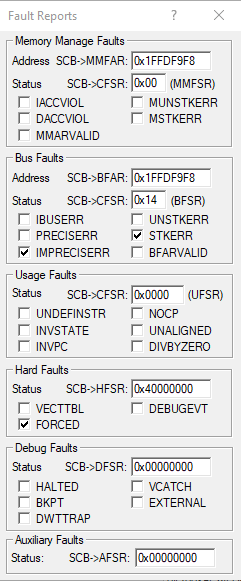
\includegraphics[width=\textwidth]{figures/keil_error_5A000.png}
        %\caption{Tiempos de convergencia en nRF52840 DK sin utilizar \textit{logs}.}
        %\label{subfig:nrf_sin_log}
    \end{subfigure}
    \hspace{1.5cm}
    \begin{subfigure}[b]{0.3\textwidth}
        \centering
        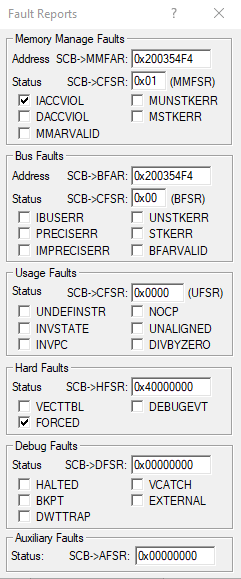
\includegraphics[width=\textwidth]{figures/keil_error_5B500.png}
        %\caption{Tiempos de convergencia en nRF52840 DK utilizando \textit{logs}.}
        %\label{subfig:nrf_con_log}
    \end{subfigure}
       \caption{Errores de manejo de memoria \textit{stack} al ejecutar McEliece348864.}
       \label{fig:mceliece-error}
\end{figure}

Dicho error se debe a que las variables utilizadas en dicha función no caben en la memoria \textit{stack}.
Las definiciones de las variables más grandes se muestran en el Código~\ref{lst:mceliece-pk-gen}.

\begin{lstlisting}[label={lst:mceliece-pk-gen},style=Cnice,firstnumber=1,caption={Variables en la función \texttt{pk\_gen}.}]
#define GFBITS 12
#define SYS_N 3488
#define SYS_T 64
#define PK_NROWS (SYS_T*GFBITS)

typedef uint16_t gf;

...

uint64_t buf[ 1 << GFBITS ];

unsigned char mat[ PK_NROWS ][ SYS_N / 8 ];

gf g[ SYS_T + 1 ]; // Goppa polynomial
gf L[ SYS_N ]; // support
gf inv[ SYS_N ];
\end{lstlisting}

La variable \texttt{buf} utiliza 32.768 bytes (0x800), lo cual ya es superior al tamaño de la memoria \textit{stack} asignada inicialmente.
La variable \texttt{mat} hace uso de 334.848 bytes (0x5\_1C00).
La variable \texttt{g} emplea 130 bytes (0x82) mientras que las variables \texttt{L} y \texttt{inv} requieren 6.976 bytes (0x1B40) cada una.
En total, el tamaño requerido de memoria \textit{stack} en esta función es de 381.650 bytes (0x5D2D2).
Por ello, se debe asignar un tamaño mínimo a la memoria \textit{stack} suficiente para llevar a cabo la ejecución del \textit{software} pero no tanta como para que no sea posible almacenar el código ejecutable, lo cual sucede al asignar 0x6\_0000 bytes a la memoria \textit{stack}.
La cantidad de memoria utilizada finalmente ha sido 0x5D800.


\subsubsection{Función de cifrado y descifrado}\label{subsubsec:mceliece-dec-enc}

Como se ha indicado en la Subsección~\ref{subsubsec:mceliece-startup}, para la ejecución de la función \texttt{pk\_gen} se ha de aumentar el tamaño de la memoria \textit{stack} casi hasta el máximo posible.
Esto cubre únicamente la generación de claves del algoritmo.
Al incluir las funciones de cifrado y descifrado se obtiene el mismo error que se recibía inicialmente para la función de generación de claves.
Esto hace que no sea viable la ejecución de la función de cifrado y descifrado del algoritmo ya que no son manejables debido al tamaño disponible de memoria.


\subsection{PQM4}\label{subsec:pqm4}




%%% Local Variables:
%%% TeX-master: "../book"
%%% End:


%%%%%%%%%%%%%%%%%%%%%%%%%%%%%%%%%%%%%%%%%%%%%%%%%%%%%%%%%%%%%%%%%%%%%%%%%%%
%
% Generic template for TFC/TFM/TFG/Tesis
%
% $Id: resultados.tex,v 1.7 2016/03/31 10:44:23 macias Exp $
%
% By:
%  + Javier Macías-Guarasa.
%    Departamento de Electrónica
%    Universidad de Alcalá
%  + Roberto Barra-Chicote.
%    Departamento de Ingeniería Electrónica
%    Universidad Politécnica de Madrid
% 
% Based on original sources by Roberto Barra, Manuel Ocaña, Jesús Nuevo, Pedro Revenga, Fernando Herránz and Noelia Hernández. Thanks a lot to all of them, and to the many anonymous contributors found (thanks to google) that provided help in setting all this up.
%
% See also the additionalContributors.txt file to check the name of additional contributors to this work.
%
% If you think you can add pieces of relevant/useful examples, improvements, please contact us at (macias@depeca.uah.es)
%
% You can freely use this template and please contribute with comments or suggestions!!!
%
%%%%%%%%%%%%%%%%%%%%%%%%%%%%%%%%%%%%%%%%%%%%%%%%%%%%%%%%%%%%%%%%%%%%%%%%%%%

\chapter{Resultados}
\label{cha:resultados}


\begin{FraseCelebre}
  \begin{Frase}
    % Si quieres ser leído más de una vez, no vaciles en borrar a menudo.
    Rem tene, verba sequentur (Si dominas el tema, las palabras vendrán solas)\footnote{Tomado de ejemplos del proyecto \texis{}.}.
  \end{Frase}
  \begin{Fuente}
    % Horacio
    Catón el Viejo
  \end{Fuente}
\end{FraseCelebre}

\section{Introducción}
\label{sec:introduccion-resultados}

En este capítulo se introducirán los resultados más relevantes del trabajo.

La estructura del capítulo es\ldots


\section{Entorno experimental}
\label{sec:entorno-experimental}

Blah, blah, blah.


\subsection{Bases de datos utilizadas}
\label{sec:bases-de-datos-1}

Blah, blah, blah.


\subsection{Métricas de calidad}
\label{sec:metricas-de-calidad}

Blah, blah, blah.

En la tabla\ref{pruebaCalc2LaTeX} pongo un ejemplo del uso del conversor de libreoffice a \LaTeX{} (cortesía de Roberto Chamorro). Para usarlo tienes que importar la macro que encontrarás en el directorio \texttt{Tools/calc2latex//calc2latex\_024\_eur\_latex}\footnote{Para ello sigue el proceso de importación que se describe en \url{http://ask.libreoffice.org/en/question/35598/where-are-lo-basic-macros-stored/}, importando Cals y cuando ejecutes la macro hazlo por el punto de entrada \texttt{Main}, después de seleccionar el rango de celdas de la tabla.}

\begin{table}[htbp]
\caption{Caption de prueba de tabla LaTeX convertida desde
  \texttt{libreoffice} con la macro \texttt{calc2latex}.}
\begin{center}
\begin{tabular}{|l|r|r|r|}
\hline
 & \multicolumn{1}{l|}{System A} & \multicolumn{1}{l|}{System B} & \multicolumn{1}{l|}{System C} \\ \hline
FA rate & 10,00\% & 5,00\% & 2,00\% \\ \hline
TA rate & 90,00\% & 85,00\% & 75,00\% \\ \hline
\end{tabular}
\end{center}
\label{pruebaCalc2LaTeX}
\end{table}




\subsection{Estrategia y metodología de experimentación}
\label{sec:estr-y-metod}

Blah, blah, blah.


\section{Resultados experimentales}
\label{sec:result-experim}

A continuación, se muestra un ejemplo de tabla simple (ver tabla \ref{tab:table1}).

\begin{table}
  % increase table row spacing, adjust to taste
  \renewcommand{\arraystretch}{1.3}
  \caption{Comparativa.}
  \label{tab:table1}
  \begin{center}
    % Some packages, such as MDW tools, offer better commands for making tables than the plain LaTeX2e tabular which is used here.
    \begin{tabular}{|c|c|c|}
      \hline
      Method & Training Time & Man-Work (\%)\\
      \hline
      Propagation model & $<$ 30 sec & 5\\
      \hline
      Manual & 9 h 30 min & 24\\
      \hline
      Automatic & 2 h & 10 8\\
      \hline
    \end{tabular}
  \end{center}
\end{table}

Cuando las tablas ocupan más de un página se debe utilizar un tipo especial de tablas denominado \texttt{longtable}. A continuación, se muestra un ejemplo del mismo (ver tabla \ref{table2}).

\begin{center}
	\begin{longtable}{|c|c|c|c|}
    \caption[Resultados de la correlación cruzada.]{Resultados de la correlación cruzada.} \label{table2} \\
    
    \hline \multicolumn{1}{|c|}{\textbf{Posición Real}} & \multicolumn{1}{c|}{\textbf{Posición estimada}} & \multicolumn{1}{c|}{\textbf{Coef. Correlación}} & \multicolumn{1}{c|}{\textbf{Acierto/Fallo}} \\ \hline 
    \endfirsthead
    
    \multicolumn{4}{c}%
    {{\bfseries \tablename\ \thetable{} -- continúa en la página anterior}} \\
    \hline \multicolumn{1}{|c|}{\textbf{Posición Real}} & \multicolumn{1}{c|}{\textbf{Posición estimada}} & \multicolumn{1}{c|}{\textbf{Coef. Correlación}} & \multicolumn{1}{c|}{\textbf{Acierto/Fallo}} \\ \hline 
    \endhead
    
    \hline \multicolumn{4}{|r|}{{Continúa en la página siguiente}} \\ \hline
    \endfoot

    \hline \hline
    \endlastfoot
    
    \hline	2P0	&	2P0	&	0,004954	&	A	\\
    \hline	2P1	&	2P4	&	0,005752	&	F	\\
    \hline	2P2	&	2P2	&	0,005461	&	A	\\
    \hline	2P3	&	2P0	&	0,004634	&	F	\\
    \hline	2P5	&	2P4	&	0,005991	&	F	\\
    \hline	2P6	&	2P16	&	0,004410	&	F	\\
    \hline	2P7	&	3P9	&	0,008038	&	F	\\
    \hline	2P8	&	3P9	&	0,003753	&	F	\\
    \hline	2P9	&	2P7	&	0,004908	&	F	\\
    \hline	2P10	&	2P10	&	0,007273	&	A	\\
    \hline	2P14	&	2P16	&	0,006485	&	F	\\
    \hline	2P15	&	2P15	&	0,004932	&	A	\\
    \hline	2P16	&	2P16	&	0,006237	&	A	\\
    \hline	2P17	&	2P15	&	0,005110	&	F	\\
    \hline	2P18	&	3P18	&	0,006235	&	F	\\
    \hline	2P19	&	3P18	&	0,004827	&	F	\\
    \hline	2P20	&	2P20	&	0,006877	&	A	\\
    \hline	2P22	&	3P18	&	0,003048	&	F	\\
    \hline	2P24	&	2P24	&	0,006833	&	A	\\
    \hline	2P25	&	2P25	&	0,004875	&	A	\\
    \hline	2P26	&	2P31	&	0,005511	&	F	\\
    \hline	2P27	&	2P28	&	0,004590	&	F	\\
    \hline	2P30	&	2P31	&	0,005576	&	F	\\
    \hline	2P31	&	2P31	&	0,007213	&	A	\\
    \hline	2P32	&	2P35	&	0,003340	&	F	\\
    \hline	2P34	&	2P34	&	0,004128	&	A	\\
    \hline	2P36	&	2P35	&	0,003329	&	F	\\
    \hline	2P37	&	2P37	&	0,003468	&	A	\\
    \hline	2P39	&	2P38	&	0,002577	&	F	\\
    \hline	2P40	&	2P43	&	0,004303	&	F	\\
    \hline	2P41	&	2P41	&	0,001573	&	A	\\
    \hline	2P42	&	2P41	&	0,000846	&	F	\\
    \hline	2P44	&	2P44	&	0,002732	&	A	\\
    \hline	2P45	&	23P45	&	0,001958	&	F	\\
    \hline	2P47	&	2P34	&	0,002869	&	F	\\
    \hline	2P48	&	2P43	&	0,004569	&	F	\\
    \hline	2P49	&	3P51	&	0,001374	&	F	\\
    \hline	2P50	&	2P34	&	0,002274	&	F	\\
    \hline	2P51	&	2P63	&	0,003931	&	F	\\
    \hline	2P52	&	2P55	&	0,003537	&	F	\\
    \hline	2P53	&	3P56	&	0,003126	&	F	\\
    \hline	2P54	&	2P67	&	0,005560	&	F	\\
    \hline	2P56	&	2P55	&	0,002817	&	F	\\
    \hline	2P57	&	2P67	&	0,006168	&	F	\\
    \hline	2P58	&	2P58	&	0,005278	&	A	\\
    \hline	2P60	&	3P66	&	0,004966	&	F	\\
    \hline	2P61	&	3P61	&	0,004748	&	A	\\
    \hline	2P64	&	2P67	&	0,005342	&	F	\\
    \hline	2P66	&	2P4	&	0,004172	&	F	\\
    \hline	2P67	&	2P67	&	0,005706	&	A	\\
    \hline	3P0	&	3P0	&	0,003674	&	A	\\
    \hline	3P61	&	2P61	&	0,003263	&	F	\\
    \hline	3P64	&	2P67	&	0,003484	&	F	\\
    \hline	3P65	&	2P67	&	0,002975	&	F	\\
    \hline	3P66	&	2P58	&	0,005029	&	F	\\
    \hline	3P67	&	3P67	&	0,003714	&	A	\\
	\end{longtable}
\end{center}

En algunas ocasiones, también resulta útil emplear el entorno
\texttt{subfigure} para añadir múltiples imágenes dentro de la misma
figura. A continuación, se muestra un ejemplo del uso en la figura
\ref{fig:fig3}. También se pueden referenciar las sub-figuras de forma
individual, por ejemplo la sub-figura \ref{fig:fig3b} (usando un método
de cita), o bien la sub-figura \ref{fig:fig3}.\subref{fig:fig3b} (usando
otro alternativo).

% For this to work you need to (in preamble.tex):
% - remove \usepackage{subfig}
% - add \usepackage{caption}
% - add \usepackage{subcaption}
\begin{figure}
  \centering
  \begin{subfigure}[b]{0.3\textwidth}
    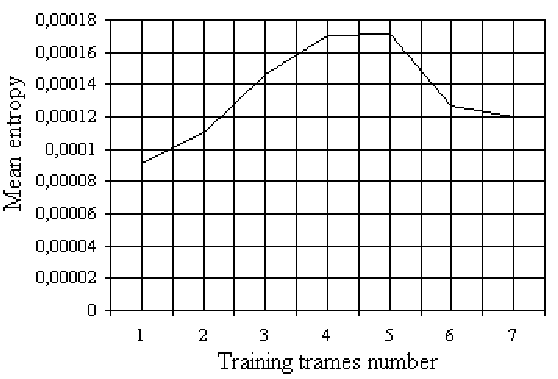
\includegraphics[width=\textwidth]{Figure2}
    \caption{Mean Entropy.}
    \label{fig:fig3a}
  \end{subfigure}%
  ~ %add desired spacing between images, e. g. ~, \quad, \qquad etc.
  % (or a blank line to force the subfigure onto a new line)
  \begin{subfigure}[b]{0.3\textwidth}
    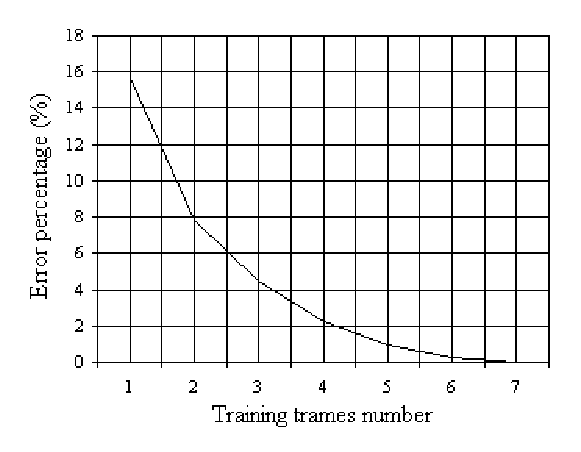
\includegraphics[width=\textwidth]{Figure3}
    \caption{Error Percentage.}
    \label{fig:fig3b}
  \end{subfigure}
  \caption{Optimal trames number in the training data set.}
  \label{fig:fig3}
\end{figure}

La figura~\ref{fig:LIdiapRoom} muestra otro ejemplo con referencias a las subfigures en el caption principal.

\begin{figure}
  \centering
  \begin{subfigure}[b]{0.30\textwidth}
    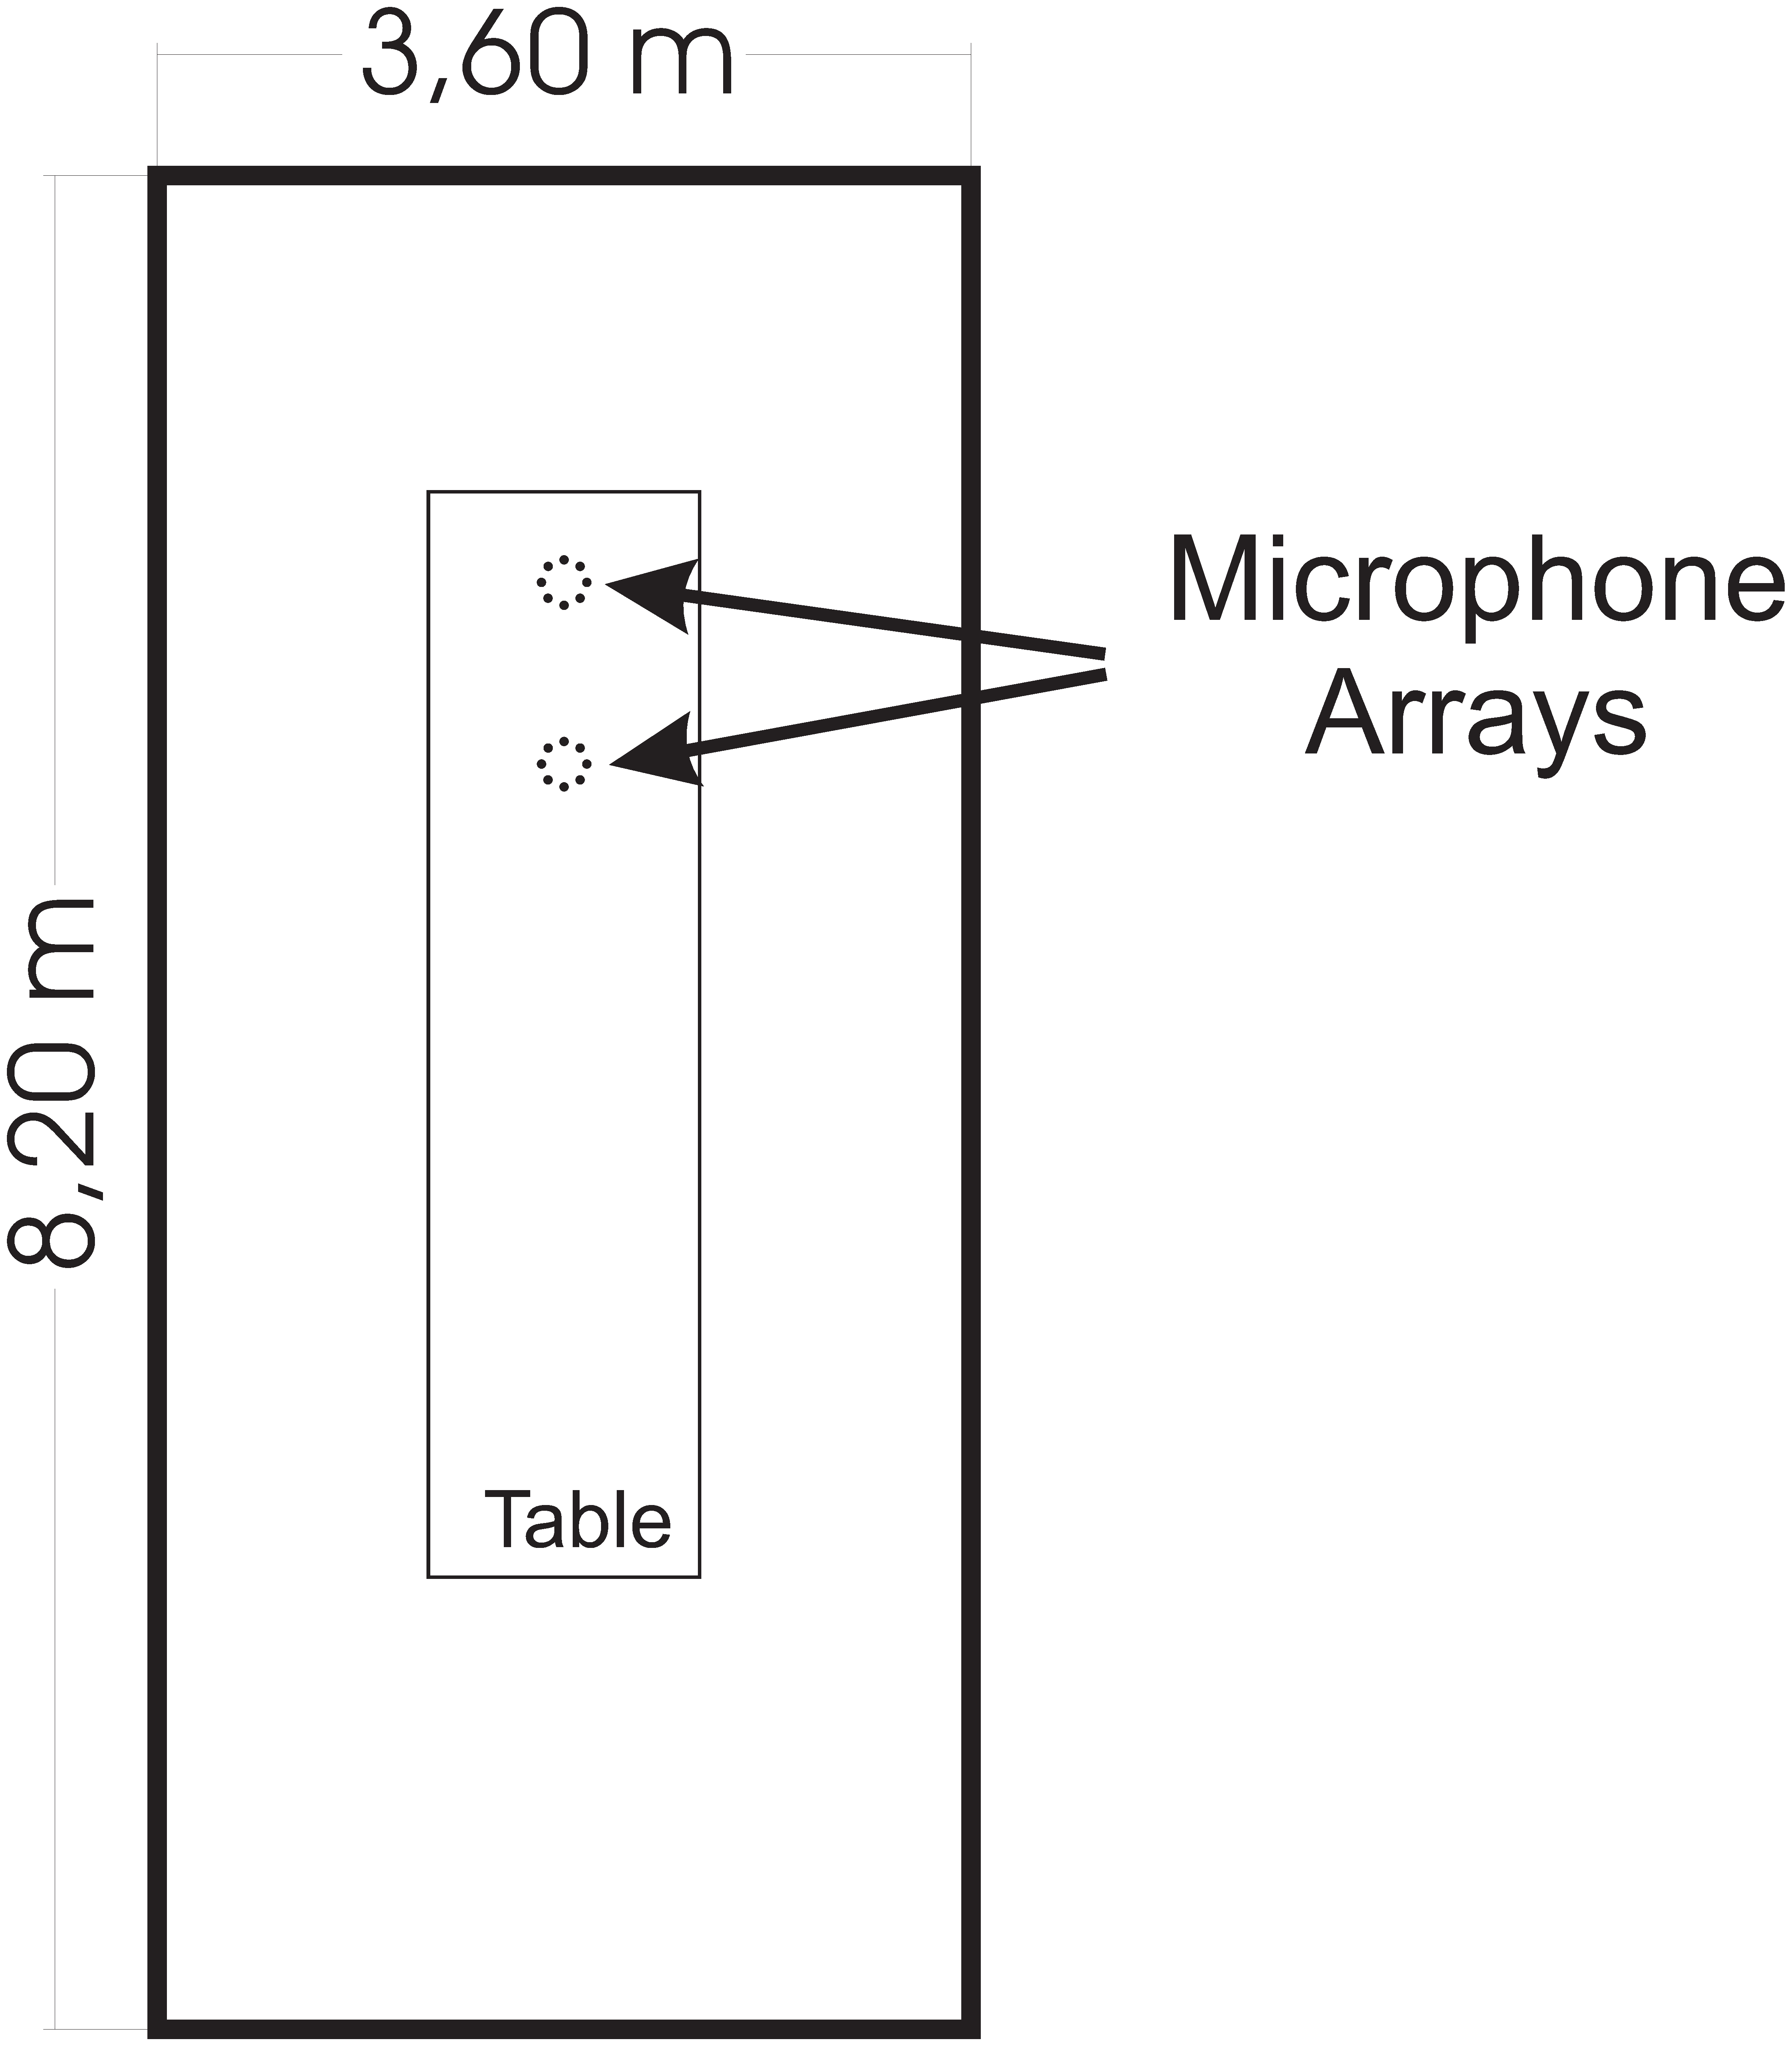
\includegraphics[width=\textwidth]{roomlayout2}
    \caption{}
    \label{fig:RoomLayout}
  \end{subfigure}%
  \qquad \qquad %add desired spacing between images, e. g. ~, \quad, \qquad, \hfill etc.
  % (or a blank line to force the subfigure onto a new line)
  \begin{subfigure}[b]{0.425\textwidth}
    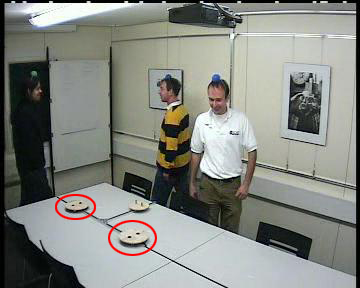
\includegraphics[width=\textwidth]{idiap-seq45-cam2.jpg}
    \caption{}
    \label{fig:RoomPicture}
  \end{subfigure}
  \caption{Idiap Smart Meeting Room for AV16.3 recordings. (\protect\subref{fig:RoomLayout}) Room layout showing the centered table, and the microphones arranged in two circular arrays. (\protect\subref{fig:RoomPicture}) Sample of recorded video frame showing the arrays area. \vspace{-0.3cm}}
  \label{fig:LIdiapRoom}
\end{figure}

Os incluimos a continuación un párrafo de un artículo en el que hacemos referencia a varias figuras y subfiguras:

\emph{The IDIAP Meeting Room (shown in figure~\ref{fig:LIdiapRoom}) is a $8.2m \times 3.6m \times 2.4m$ rectangular space containing a centrally located $4.8m \times 1.2m$ rectangular table, on top of which two circular microphone arrays of $10 cm$ radius are located, each of them composed by 8 microphones. The centers of the two arrays are separated by $80 cm$ and the origin of coordinates is located in the middle point between the two arrays. The arrays can be also seen in figures~\ref{fig:simureal_positions}.\subref{fig:Simulated_positions}, ~\ref{fig:simureal_positions}.\subref{fig:real_positions_short}, and ~\ref{fig:simureal_positions}.\subref{fig:real_positions_long}, in which only the relevant section of the room is displayed, each one showing different scenarios that were used in the experiments. A detailed description of the meeting room can be found in~\cite{moore2002}.}

\begin{figure}
  \centering
  \begin{subfigure}[t]{0.3\textwidth}
    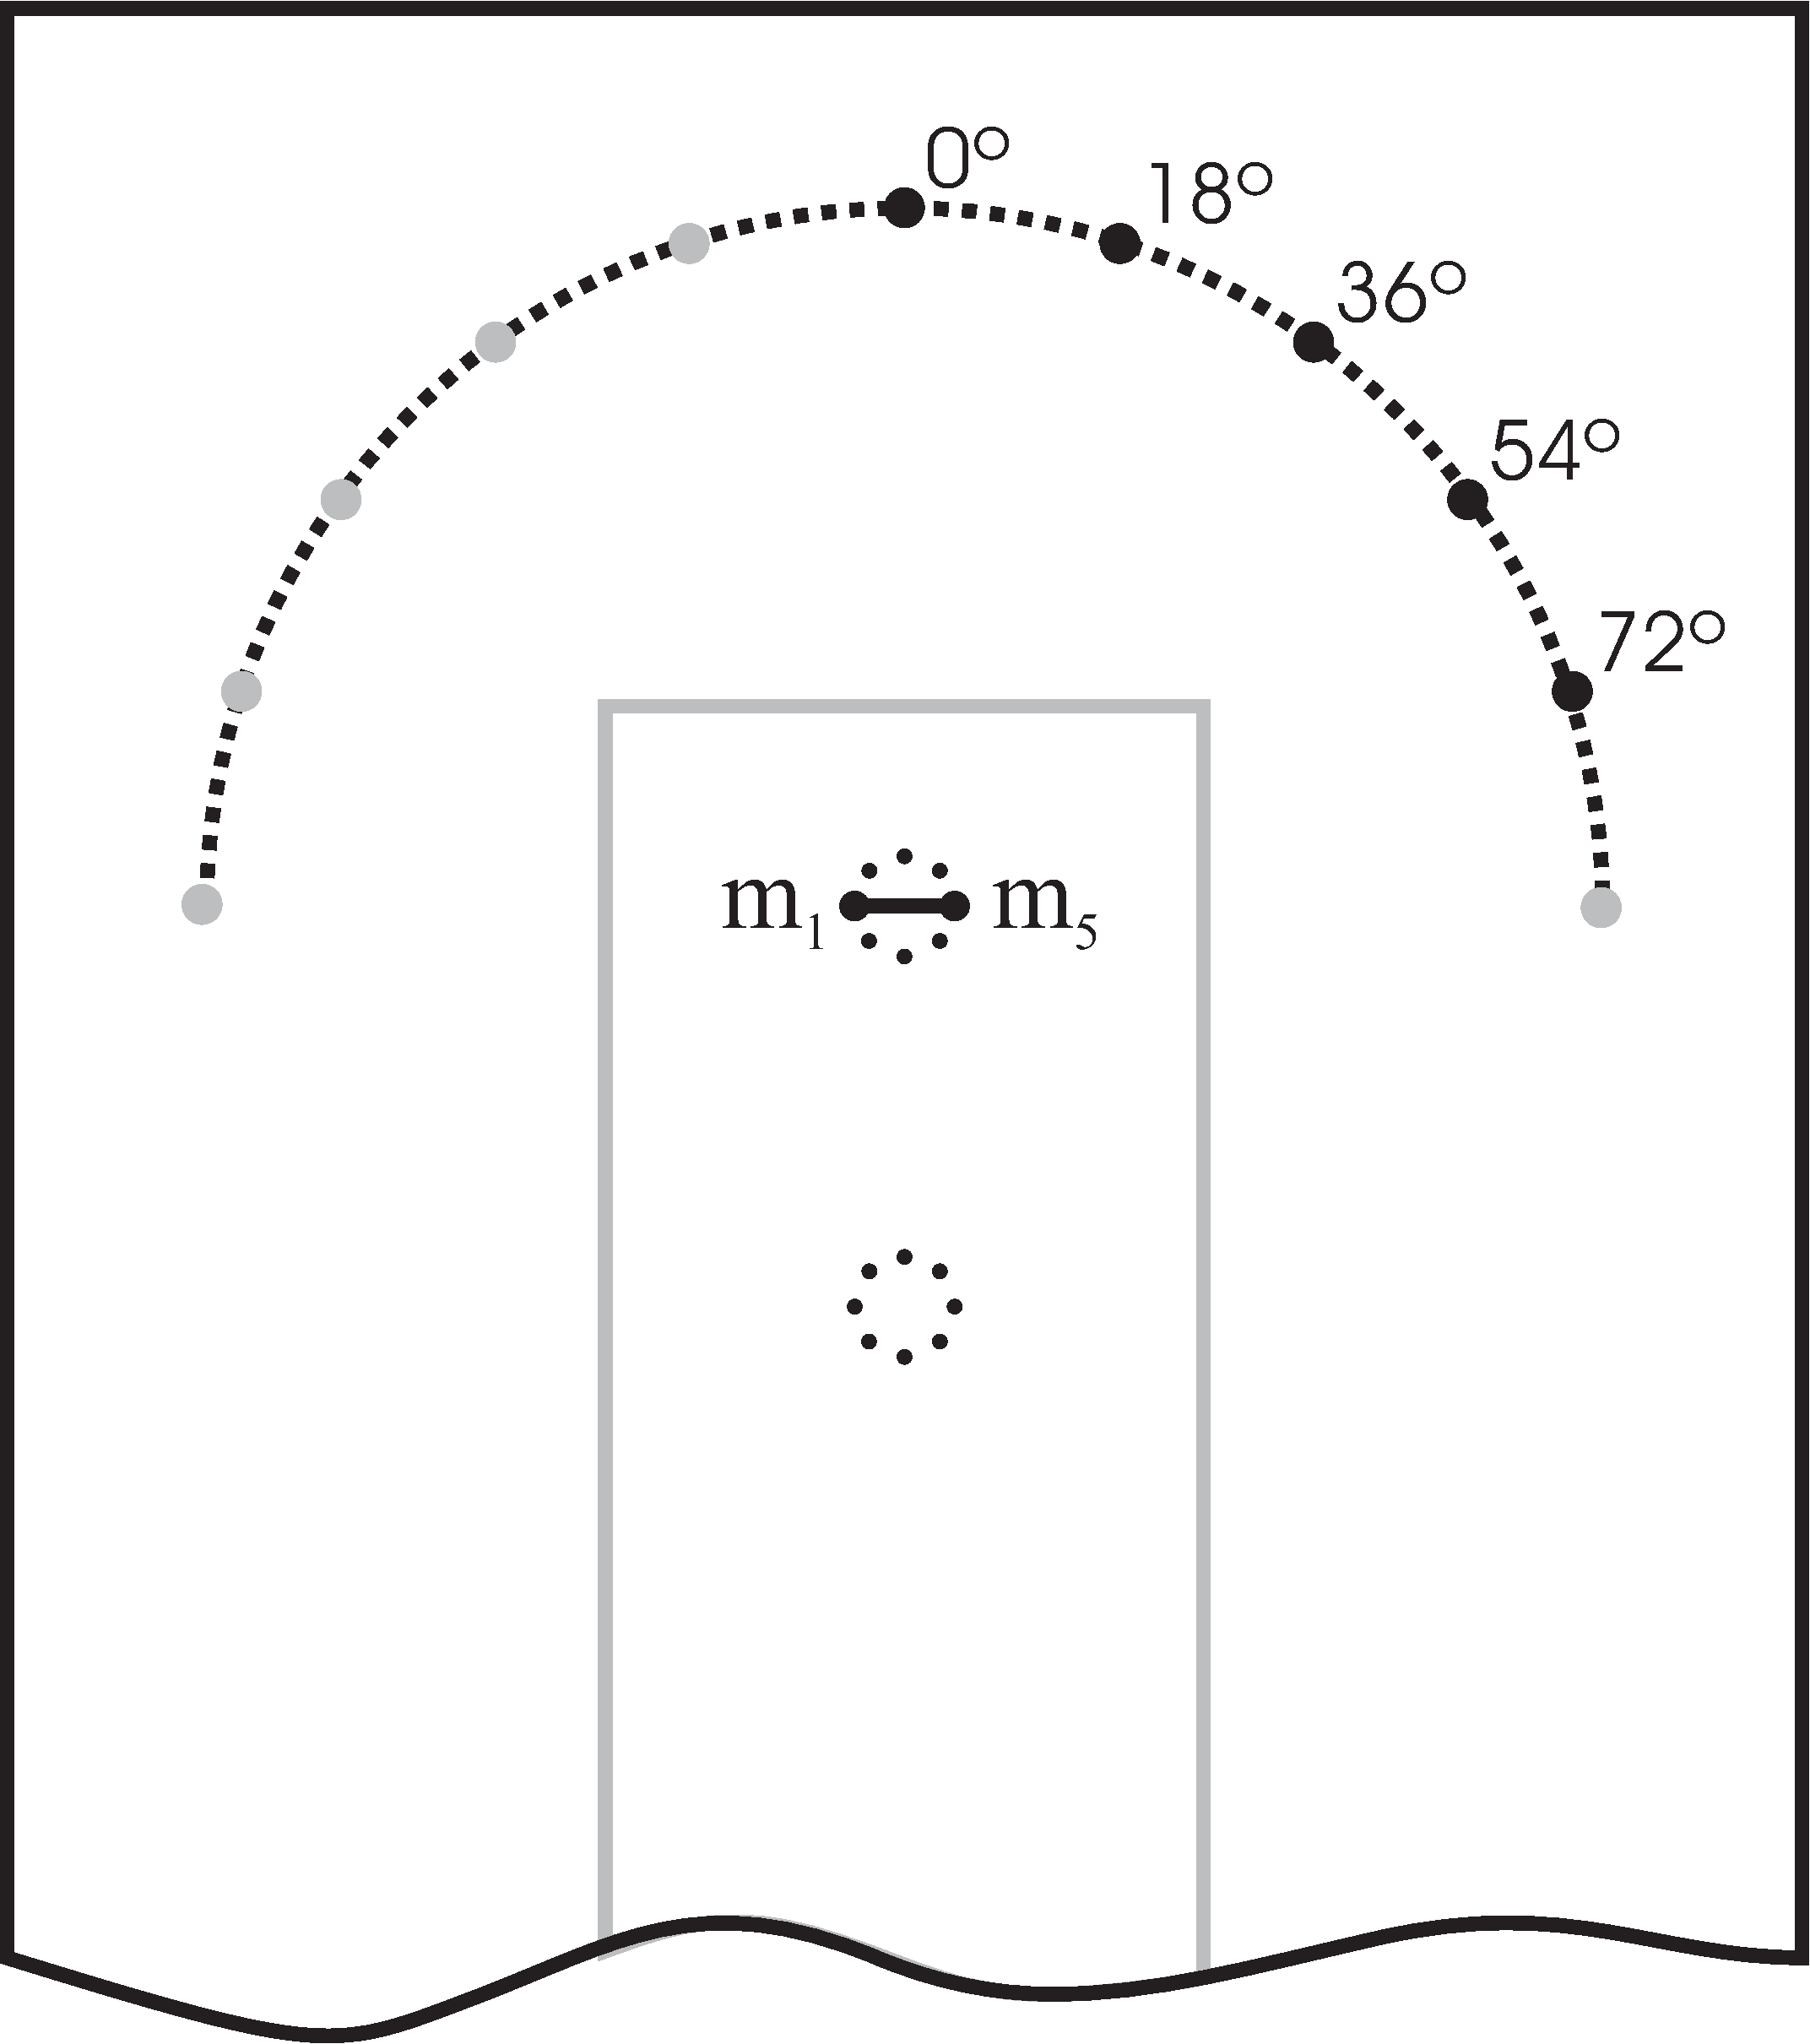
\includegraphics[width=\textwidth]{angular2-short-improved}
    \caption{For validation\\with simulated data.}
    \label{fig:Simulated_positions}
  \end{subfigure}
~%add desired spacing between images, e. g. ~, \quad, \qquad,
  % \hfill etc.
  % (or a blank line to force the subfigure onto a new line)
  \begin{subfigure}[t]{0.3\textwidth}
    
\includegraphics[width=\textwidth]{positions1-short-improved}
    \caption{For validation\\with real data and microphone pairs with $20~cm$ spacing.}
    \label{fig:real_positions_short}
  \end{subfigure}
  ~
  \begin{subfigure}[t]{0.3\textwidth}
    
\includegraphics[width=\textwidth]{positions2-short-improved}
    \caption{For validation\\with real data and microphone pairs with
      $82.46~cm$ spacing.}
    \label{fig:real_positions_long}
  \end{subfigure}
  \caption{Geometrical details for the experiments carried out. Only the
    relevant section of the room is shown, and microphone pairs are
    connected by solid lines.}
  \label{fig:simureal_positions}
\end{figure}

En la figura~\ref{fig:Sim_angles} mostramos un ejemplo de varias
figuras organizadas de forma un poco más complejo.

\begin{figure}
  \centering
  \begin{subfigure}[b]{0.3\textwidth}
    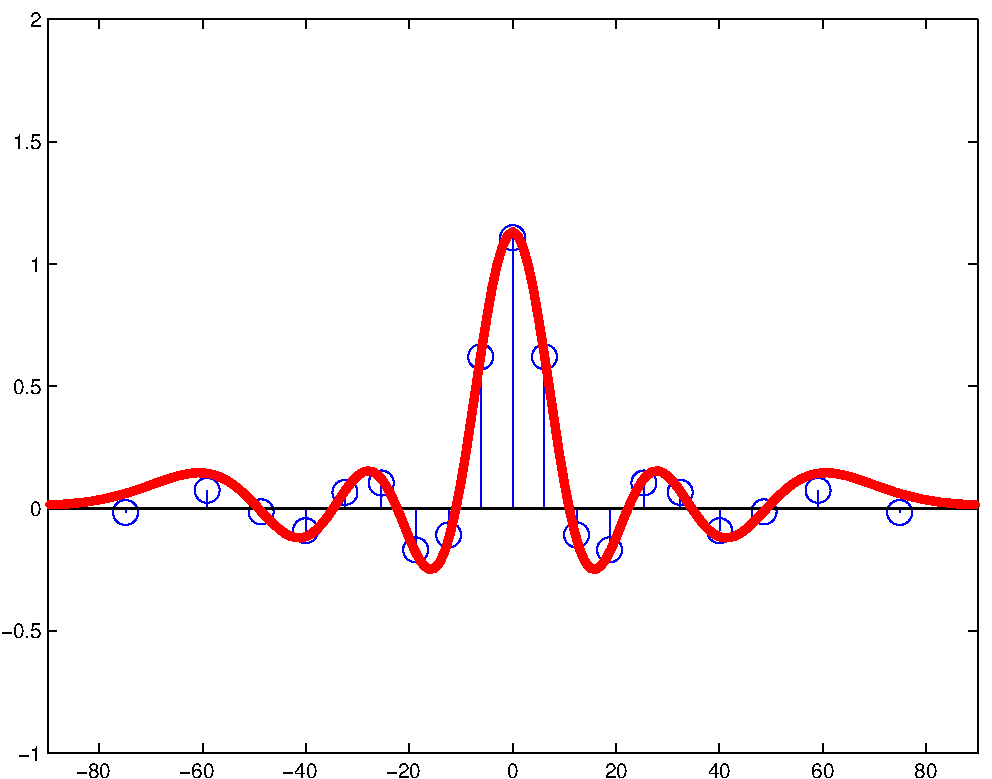
\includegraphics[width=\textwidth]{Sim_seg025_ang090}
    \caption{$0^{\circ}$}
    \label{fig:Sim_ang090}
  \end{subfigure}
  % add desired spacing between images, e. g. ~, \quad, \qquad etc.
  % (or a blank line to force the subfigure onto a new line)

  \begin{subfigure}[b]{0.3\textwidth}
    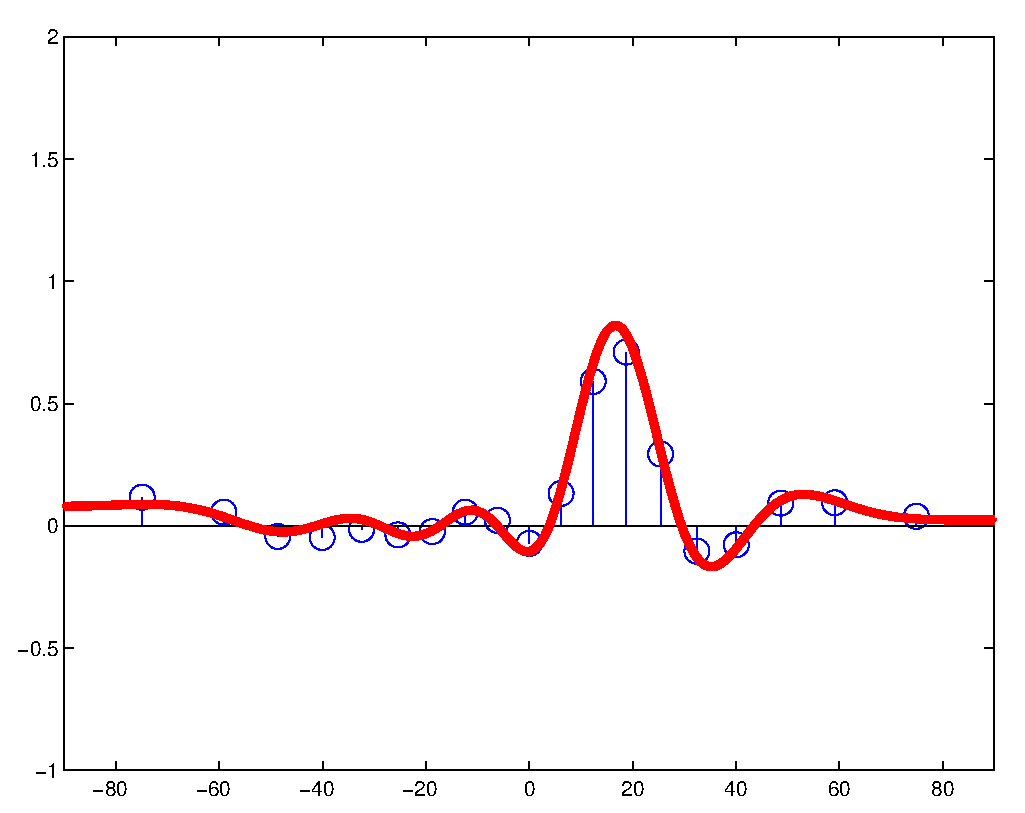
\includegraphics[width=\textwidth]{Sim_seg025_ang108}
    \caption{$18^{\circ}$}
    \label{fig:Sim_ang108}
  \end{subfigure}
  % add desired spacing between images, e. g. ~, \quad, \qquad etc.
  % (or a blank line to force the subfigure onto a new line)
  \begin{subfigure}[b]{0.3\textwidth}
    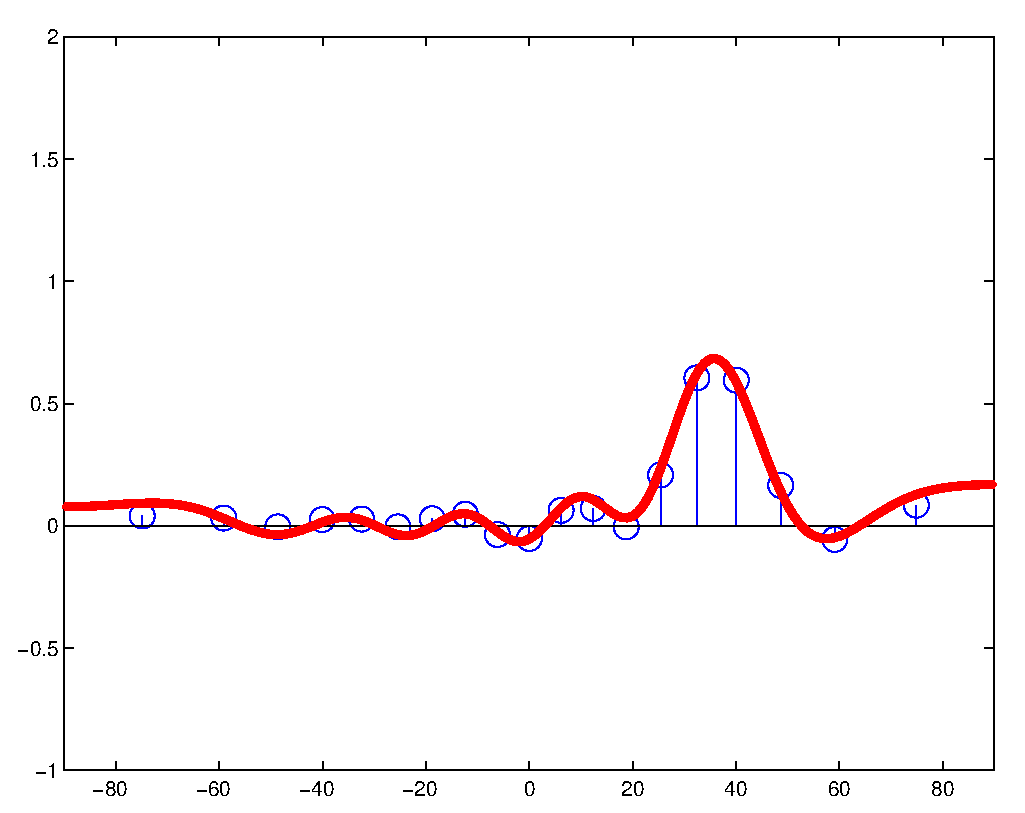
\includegraphics[width=\textwidth]{Sim_seg025_ang126}
    \caption{$36^{\circ}$}
    \label{fig:Sim_ang126}
  \end{subfigure}
  % add desired spacing between images, e. g. ~, \quad, \qquad etc.
  % (or a blank line to force the subfigure onto a new line)
  \begin{subfigure}[b]{0.3\textwidth}
    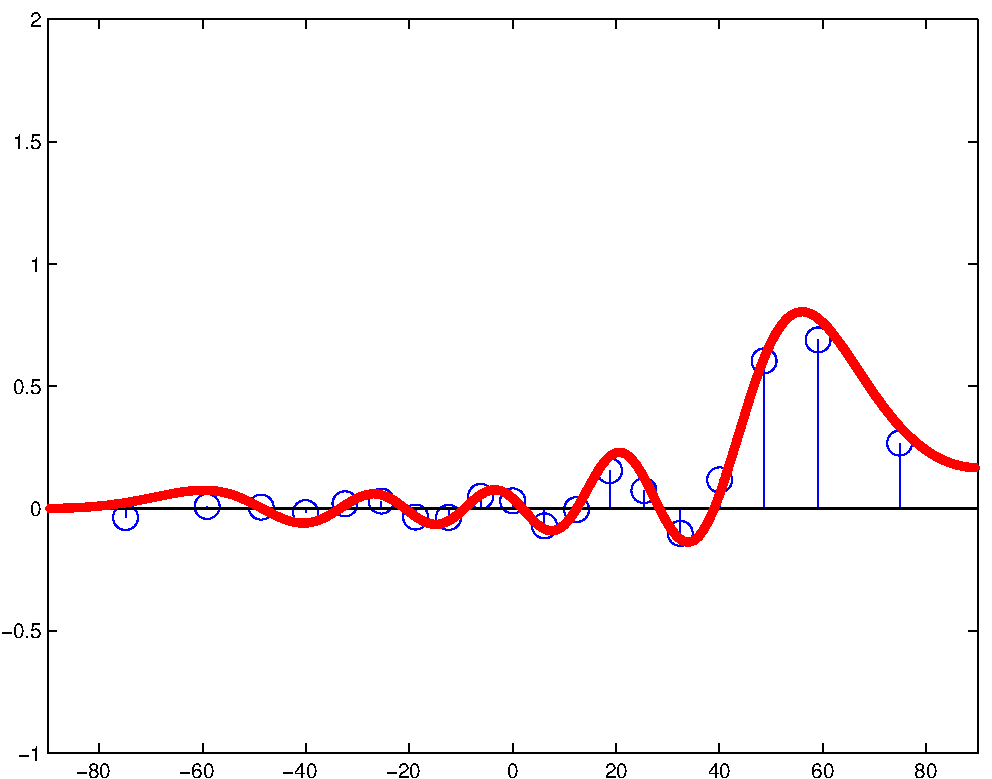
\includegraphics[width=\textwidth]{Sim_seg025_ang144}
    \caption{$54^{\circ}$}
    \label{fig:Sim_ang144}
  \end{subfigure}
  % add desired spacing between images, e. g. ~, \quad, \qquad etc.
  % (or a blank line to force the subfigure onto a new line)

  \begin{subfigure}[b]{0.3\textwidth}
    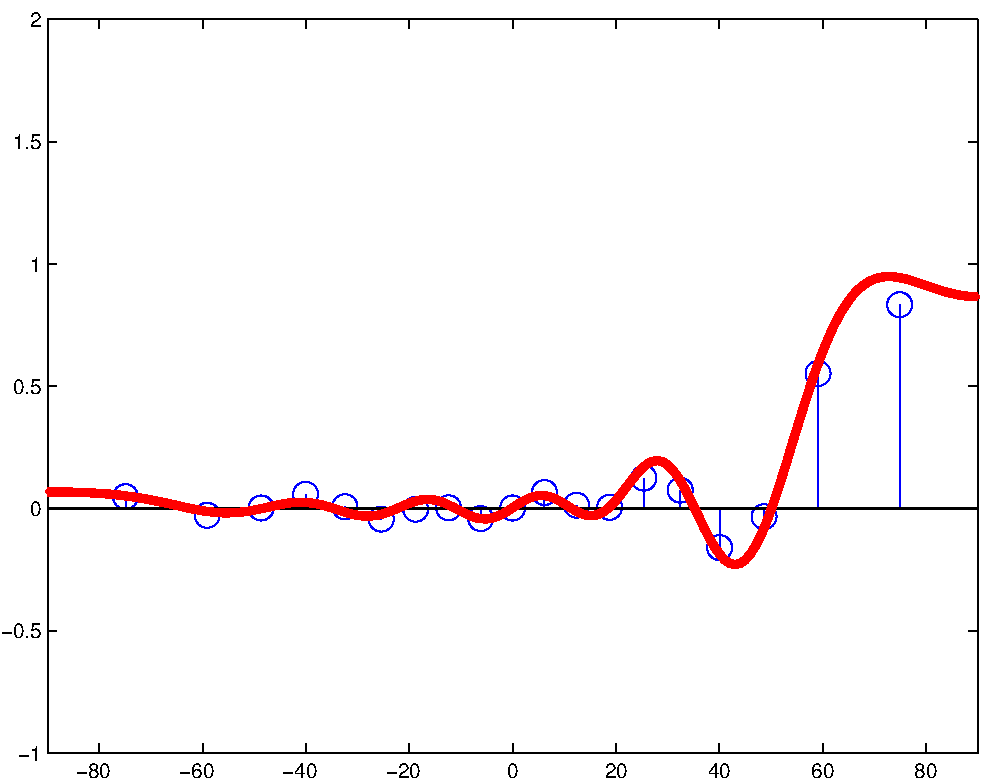
\includegraphics[width=\textwidth]{Sim_seg025_ang162}
    \caption{$72^{\circ}$}
    \label{fig:Sim_ang162}
  \end{subfigure}

  \caption{Comparison between the steered power response generated by the model (solid line) and that calculated using simulated waveforms in the AV16.3 environment (stems). Results for the speaker in given angles and the array steered from -90º to +90º are shown.}
  \label{fig:Sim_angles}
\end{figure}

También es posible incluir el código de una figura en un fichero \texttt{.tex} independiente (para hacer más legible el código del documento principal). Un ejemplo lo tenéis a continuación, incluyendo el texto en inglés del documento original:

\emph{Figure~\ref{fig:SRPvsPatternSelected} includes the results of the comparison, for several speaker positions (1, 2, 4, 6, 8 and 16, emphasized in figure~\ref{fig:simureal_positions}.\subref{fig:real_positions_short}), and selected to provide different acoustic situations, both in terms of distance and angular position with respect to the arrays. All the graphics show the acoustic power map (predicted or calculated) for a regular two-dimensional grid of $10~cm$. The plot is provided from a top view of the room, spanning the full plan at a height of $61~cm$ above the microphone arrays (this height was the ground truth one for sequence 01). For each speaker position shown, three graphics are plotted:}

\begin{itemize}
  \item \emph{The graphics on the left show the SRP-PHAT acoustic power maps generated by the proposed model (for example, the left graphic in figure~\ref{fig:SRPvsPatternSelected}.\subref{fig:SRPvsModel_Fo1500_position1} for position 1).}
  \item \emph{The graphics in the middle show the real SRP-PHAT acoustic power maps calculated using the real acoustic waveforms (for example, the middle graphic in figure~\ref{fig:SRPvsPatternSelected}.\subref{fig:SRPvsModel_Fo1500_position1} for position 1), for a single selected frame.}
  \item \emph{The graphics on the right show the average real SRP-PHAT acoustic power maps, averaging for all the frames in which the user was in the given position (for example, the right graphic in figure~\ref{fig:SRPvsPatternSelected}.\subref{fig:SRPvsModel_Fo1500_position1} for position 1).}
\end{itemize}

\emph{The green point represents the real (ground truth) speaker position, and the black dots represent the positions of the four microphones used. The hyperbolic shapes found in the figure are consistent with the fact that the place of points with equal acoustic power value, for a given microphone pair, is a hyperbola (in our two-dimensional case, being a hyperboloid of revolution in the three-dimensional case).}

\emph{From figure~\ref{fig:SRPvsPatternSelected}, it can clearly be seen that, again, the predictions closely match the results with real data for the different acoustic conditions, even when the simulations are using fixed and frequency independent average reflection coefficients, and that the acoustic model is based on the simplistic image method model.}

\begin{figure}
  \centering
  \begin{subfigure}[t]{0.47\textwidth}
    \begin{minipage}[t]{\textwidth}
      \begin{subfigure}[t]{0.3\textwidth}
        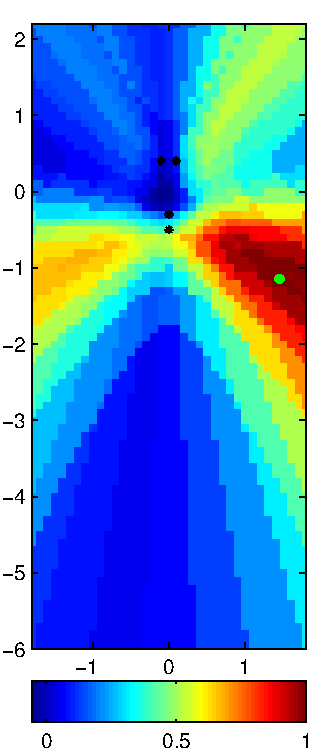
\includegraphics[width=\textwidth]{Pattern_Fo1500_pos01}
        %\caption{SRP Model for pos. 1}
        \label{fig:Pattern_Fo1500_pos01}
      \end{subfigure}
      % ~ %add desired spacing between images, e. g. ~, \quad, \qquad,
      % \hfill etc.
      % (or a blank line to force the subfigure onto a new line)
      \begin{subfigure}[t]{0.3\textwidth}
        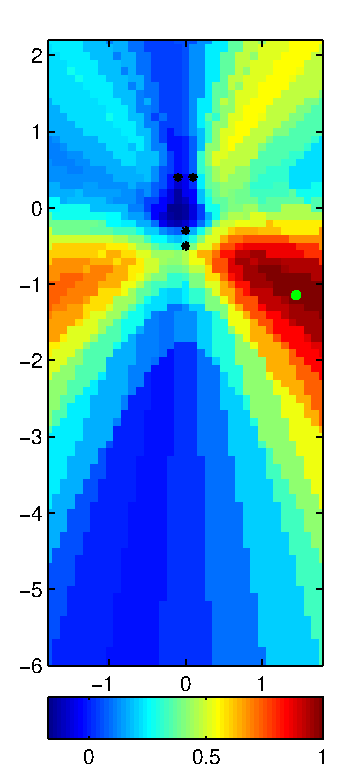
\includegraphics[width=\textwidth]{SRP_Fo1500_frame003_pos01}
        % \caption{Real SRP for pos.  1}
        \label{fig:SRP_Fo1500_pos01}
      \end{subfigure}
      % ~ %add desired spacing between images, e. g. ~, \quad, \qquad,
      % \hfill etc.
      % (or a blank line to force the subfigure onto a new line)
      \begin{subfigure}[t]{0.3\textwidth}
        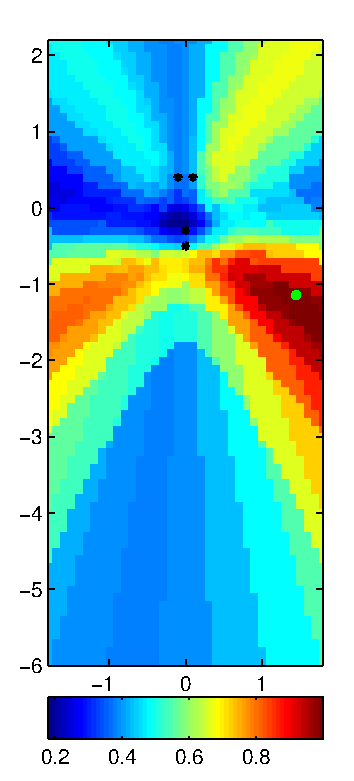
\includegraphics[width=\textwidth]{SRP_Fo1500_mean_pos01}
        % \caption{Avg. SRP for pos. 1}
        \label{fig:SRP_Fo1500_mean_pos01}
      \end{subfigure}
      \vspace{\verticalSpacingSRPMaps}
      \caption{\centering For position 1}
      \label{fig:SRPvsModel_Fo1500_position1}
      \vspace{0.25cm}
    \end{minipage}
  \end{subfigure}
  ~% \quad % between 1 and 2 %add desired spacing between images, e. g. ~, \quad, \qquad,
  % \hfill etc.
  % (or a blank line to force the subfigure onto a new line)
  \begin{subfigure}[t]{0.47\textwidth}
    \begin{minipage}[t]{\textwidth}
      \begin{subfigure}[t]{0.3\textwidth}
        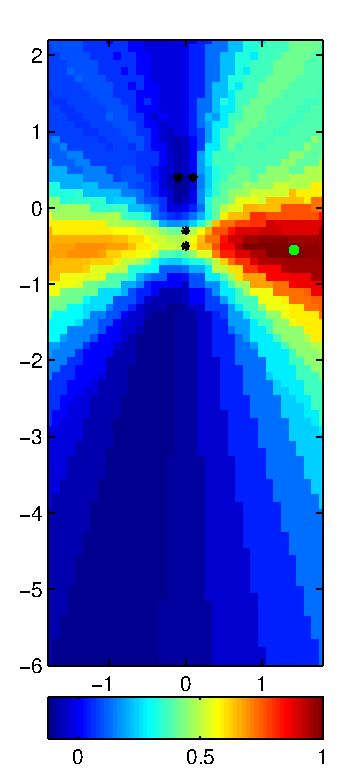
\includegraphics[width=\textwidth]{Pattern_Fo1500_pos02}
        % \caption{SRP Model for pos. 2}
        \label{fig:Pattern_Fo1500_pos02}
      \end{subfigure}
      % ~ %add desired spacing between images, e. g. ~, \quad, \qquad,
      % \hfill etc.
      % (or a blank line to force the subfigure onto a new line)
      \begin{subfigure}[t]{0.3\textwidth}
        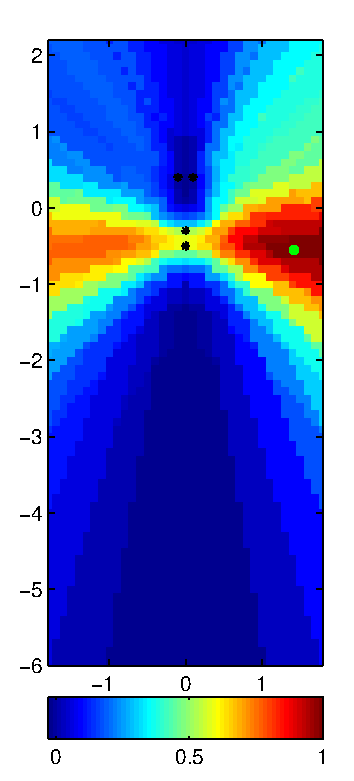
\includegraphics[width=\textwidth]{SRP_Fo1500_frame161_pos02}
        % \caption{Real SRP for pos.  2\\}
        \label{fig:SRP_pos02}
      \end{subfigure}
      % ~ %add desired spacing between images, e. g. ~, \quad, \qquad,
      % \hfill etc.
      % (or a blank line to force the subfigure onto a new line)
      \begin{subfigure}[t]{0.3\textwidth}
        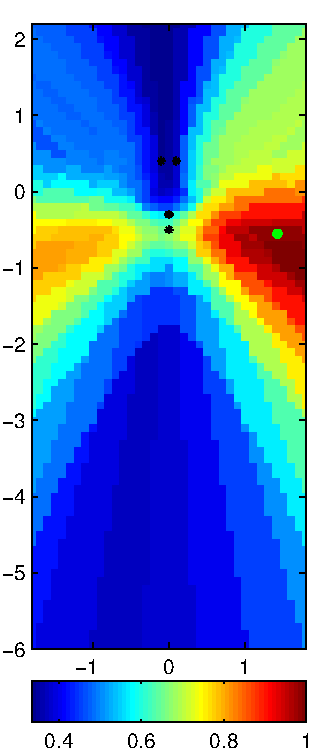
\includegraphics[width=\textwidth]{SRP_Fo1500_mean_pos02}
        % \caption{Avg. SRP for pos. 2}
        \label{fig:SRP_Fo1500_mean_pos02}
      \end{subfigure}
      \vspace{\verticalSpacingSRPMaps}
      \caption{\centering For position 2}
      \vspace{0.25cm}
    \end{minipage}
  \end{subfigure}

  \begin{subfigure}[t]{0.47\textwidth}
    \begin{minipage}[t]{\textwidth}
      \begin{subfigure}[t]{0.3\textwidth}
        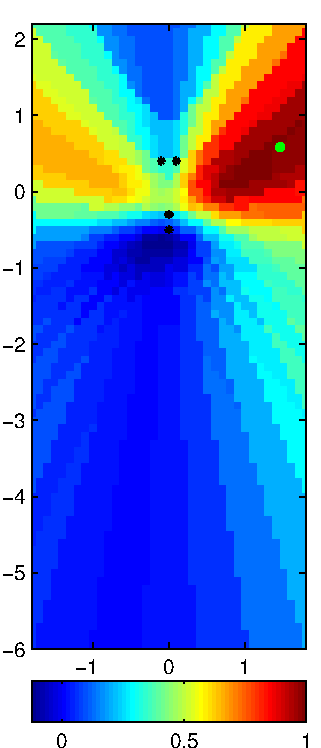
\includegraphics[width=\textwidth]{Pattern_Fo1500_pos04}
        % \caption{SRP Model for pos. 4}
        \label{fig:Pattern_Fo1500_pos04}
      \end{subfigure}
      % ~ %add desired spacing between images, e. g. ~, \quad, \qquad,
      % \hfill etc.
      % (or a blank line to force the subfigure onto a new line)
      \begin{subfigure}[t]{0.3\textwidth}
        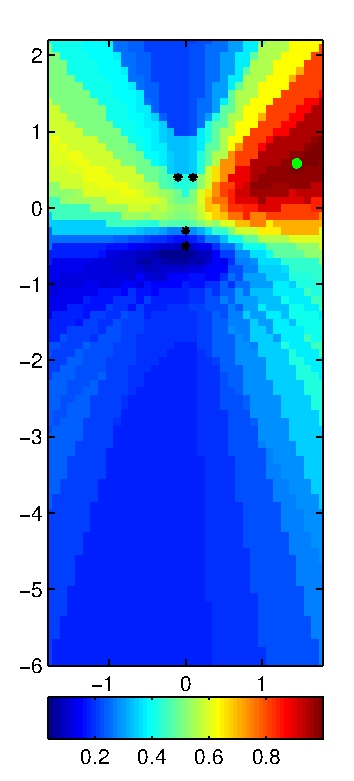
\includegraphics[width=\textwidth]{SRP_Fo1500_frame464_pos04}
        % \caption{Real SRP for pos.  4\\}
        \label{fig:SRP_pos04}
      \end{subfigure}
      % ~ %add desired spacing between images, e. g. ~, \quad, \qquad,
      % \hfill etc.
      % (or a blank line to force the subfigure onto a new line)
      \begin{subfigure}[t]{0.3\textwidth}
        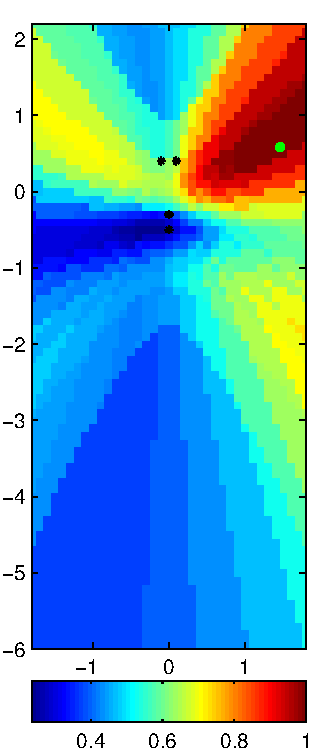
\includegraphics[width=\textwidth]{SRP_Fo1500_mean_pos04}
        % \caption{Avg. SRP for pos. 4}
        \label{fig:SRP_Fo1500_mean_pos04}
      \end{subfigure}
      \vspace{\verticalSpacingSRPMaps}
      \caption{\centering For position 4}
      \vspace{0.25cm}
    \end{minipage}
  \end{subfigure}
  ~%  \qquad % between 4 and 6 %add desired spacing between images, e. g. ~, \quad, \qquad,
  % \hfill etc.
  % (or a blank line to force the subfigure onto a new line)
  \begin{subfigure}[t]{0.47\textwidth}
    \begin{minipage}[t]{\textwidth}
      \begin{subfigure}[t]{0.3\textwidth}
        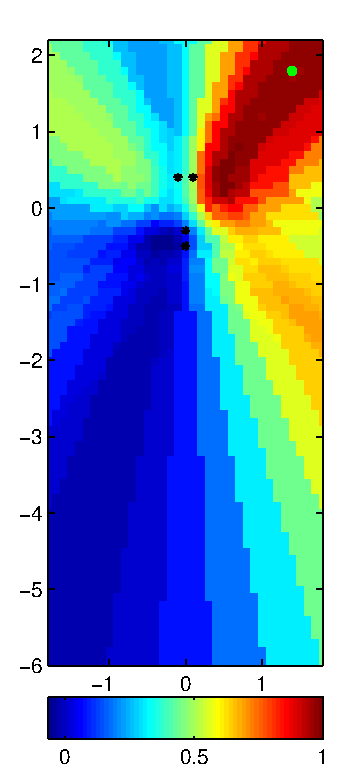
\includegraphics[width=\textwidth]{Pattern_Fo1500_pos06}
        % \caption{SRP Model for pos. 6}
        \label{fig:Pattern_Fo1500_pos06}
      \end{subfigure}
      % ~ %add desired spacing between images, e. g. ~, \quad, \qquad,
      % \hfill etc.
      % (or a blank line to force the subfigure onto a new line)
      \begin{subfigure}[t]{0.3\textwidth}
        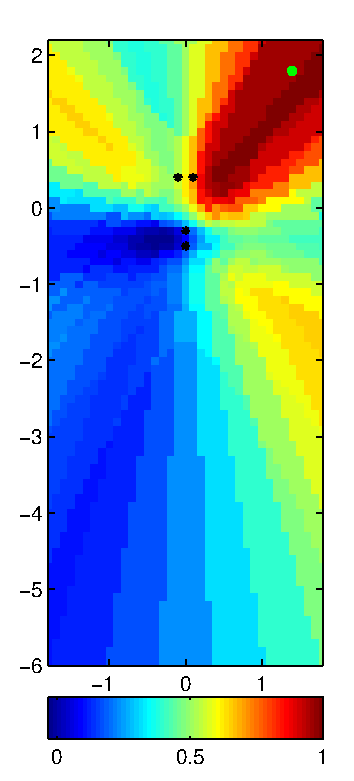
\includegraphics[width=\textwidth]{SRP_Fo1500_frame809_pos06}
        % \caption{Real SRP for pos.  6\\}
        \label{fig:SRP_pos06}
      \end{subfigure}
      % ~ %add desired spacing between images, e. g. ~, \quad, \qquad,
      % \hfill etc.
      % (or a blank line to force the subfigure onto a new line)
      \begin{subfigure}[t]{0.3\textwidth}
        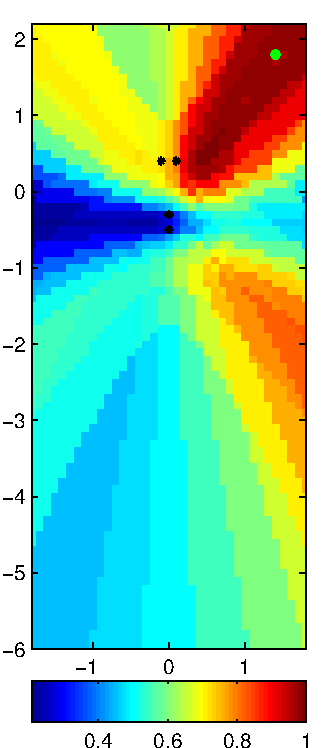
\includegraphics[width=\textwidth]{SRP_Fo1500_mean_pos06}
        % \caption{Avg. SRP for pos. 6}
        \label{fig:SRP_Fo1500_mean_pos06}
      \end{subfigure}
      \vspace{\verticalSpacingSRPMaps}
      \caption{\centering For position 6}
      \vspace{0.25cm}
    \end{minipage}
  \end{subfigure}

  \begin{subfigure}[t]{0.47\textwidth}
    \begin{minipage}[t]{\textwidth}
      \begin{subfigure}[t]{0.3\textwidth}
        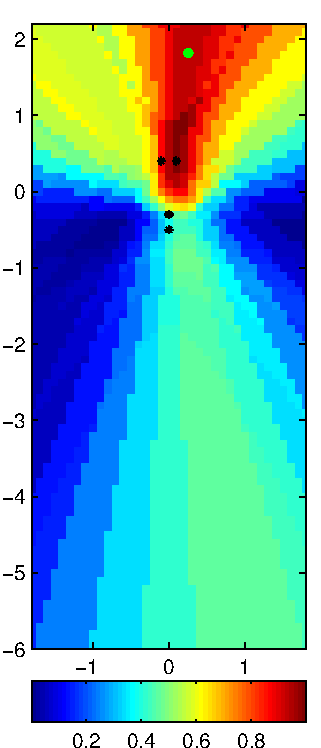
\includegraphics[width=\textwidth]{Pattern_Fo1500_pos08}
        % \caption{SRP Model for pos. 8}
        \label{fig:Pattern_Fo1500_pos08}
      \end{subfigure}
      % ~ %add desired spacing between images, e. g. ~, \quad, \qquad,
      % \hfill etc.
      % (or a blank line to force the subfigure onto a new line)
      \begin{subfigure}[t]{0.3\textwidth}
        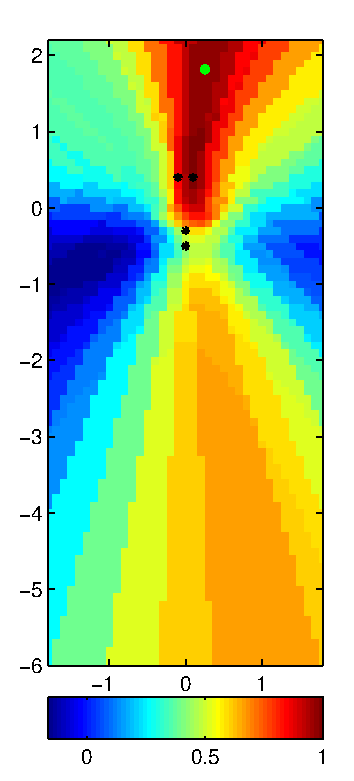
\includegraphics[width=\textwidth]{SRP_Fo1500_frame1127_pos08}
        % \caption{Real SRP for pos.  8\\}
        \label{fig:SRP_pos08}
      \end{subfigure}
      % ~ %add desired spacing between images, e. g. ~, \quad, \qquad,
      % \hfill etc.
      % (or a blank line to force the subfigure onto a new line)
      \begin{subfigure}[t]{0.3\textwidth}
        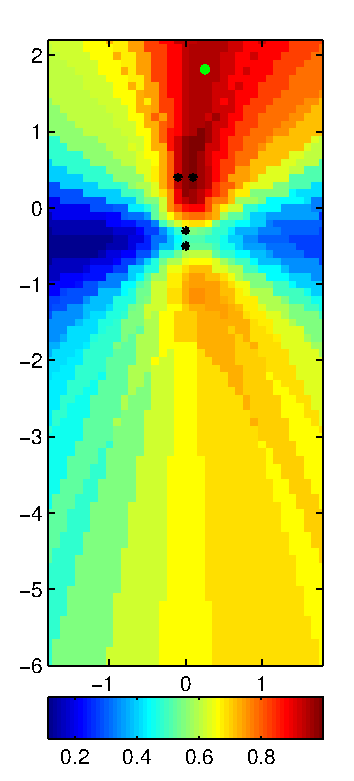
\includegraphics[width=\textwidth]{SRP_Fo1500_mean_pos08}
        % \caption{Avg. SRP for pos. 8}
        \label{fig:SRP_Fo1500_mean_pos08}
      \end{subfigure}
      \vspace{\verticalSpacingSRPMaps}
      \caption{\centering For position 8}
      \vspace{0.25cm}
    \end{minipage}
  \end{subfigure}
  ~%  \qquad % between 8 and 16 %add desired spacing between images, e. g. ~, \quad, \qquad,
  % \hfill etc.
  % (or a blank line to force the subfigure onto a new line)
  \begin{subfigure}[t]{0.47\textwidth}
    \begin{minipage}[t]{\textwidth}
      \begin{subfigure}[t]{0.3\textwidth}
        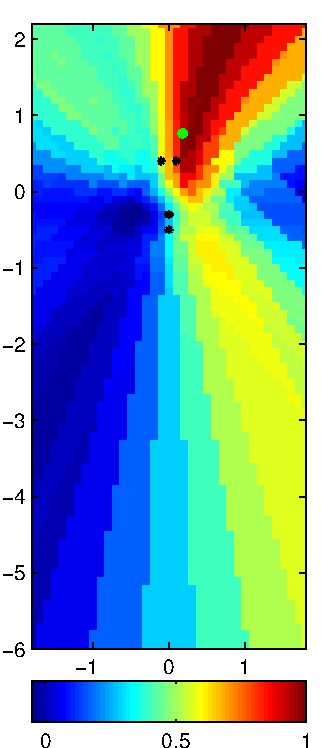
\includegraphics[width=\textwidth]{Pattern_Fo1500_pos16}
        % \caption{SRP Model for pos. 16}
        \label{fig:Pattern_Fo1500_pos16}
      \end{subfigure}
      % ~ %add desired spacing between images, e. g. ~, \quad, \qquad,
      % \hfill etc.
      % (or a blank line to force the subfigure onto a new line)
      \begin{subfigure}[t]{0.3\textwidth}
        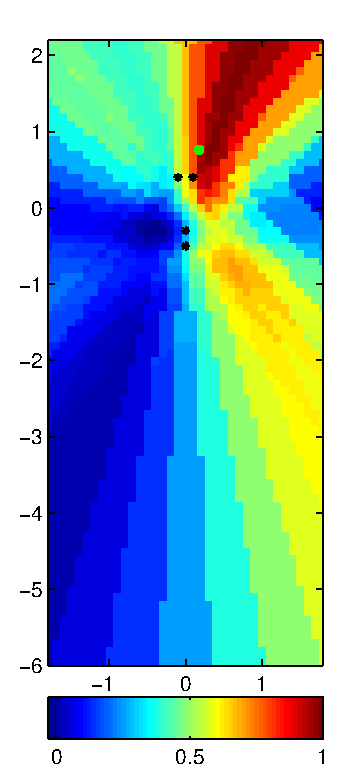
\includegraphics[width=\textwidth]{SRP_Fo1500_frame2518_pos16}
        % \caption{Real SRP for pos. 16\\}
        \label{fig:SRP_pos16}
      \end{subfigure}
      % ~ %add desired spacing between images, e. g. ~, \quad, \qquad,
      % \hfill etc.
      % (or a blank line to force the subfigure onto a new line)
      \begin{subfigure}[t]{0.3\textwidth}
        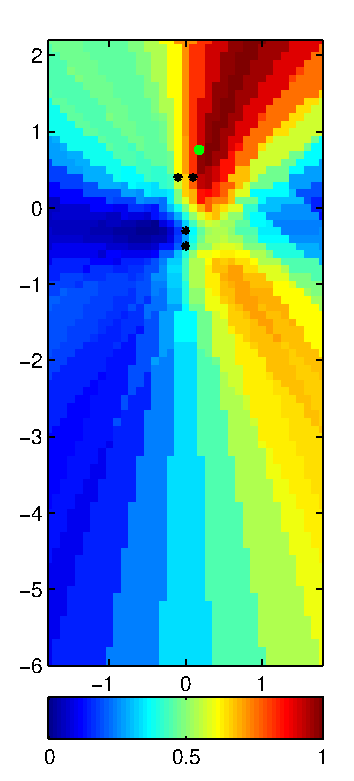
\includegraphics[width=\textwidth]{SRP_Fo1500_mean_pos16}
        % \caption{Avg. SRP for pos. 16}
        \label{fig:SRP_Fo1500_mean_pos16}
      \end{subfigure}
      \vspace{\verticalSpacingSRPMaps}
      \caption{\centering For position 16}
      \vspace{0.25cm}
    \end{minipage}
  \end{subfigure}
  \caption{Comparison between the SRP-PHAT map predicted by the model
    (left graphics),
    the real SRP-PHAT map (middle graphics), and the average (real)
    SRP-PHAT map (right graphics), for
    several speaker positions ($f_0=1.5~KHz$). See
    figure~~\ref{fig:simureal_positions}.\subref{fig:real_positions_short}
    for geometrical references.}
  \label{fig:SRPvsPatternSelected}
\end{figure}
 

\begin{wrapfigure}{r}{0.5\textwidth} 
\vspace{-20pt}
  \begin{center}
    \includegraphics[width=0.4\textwidth]{Figure1}
    \caption{Ejemplo de figura con wrapfigure.}
    \label{fig:wrapfigure1}
  \end{center}
  \vspace{-20pt}
  \vspace{1pt}
\end{wrapfigure} 

Otra posibilidad es utilizar el entorno \texttt{wrapfig} para hacer que el texto bordee a las figuras, como en la figura~\ref{fig:wrapfigure1}. Añado ahora unas líneas de loren ipsum para que lo veáis bien. \lipsum[1-1]

% \lipsum[1-4]
% \begin{wrapfigure}{R}{5cm}
% \centering
% \rule{3cm}{7cm}
% \end{wrapfigure}
% \lipsum[1-6]

Incluso podemos poner una tabla ``apaisada'', como en la \ref{tab:tablas2006}, donde se muestra un resumen de los resultados obtenidos en una serie de experimentos de localización de locutores.

\clearpage
% \begin{table}[H]\centering
\begin{sidewaystable}[hbtp]
  \begin{center}

    \begin{tabular}{||l|c|c|c|c|c||}
      \hline \hline
      & UKA & ITC & AIT & UPC & IBM\\
      \hline
      \hline
      Pcor & $57.0\pm1.4\%$ & $84.0\pm3.3\%$ & $47.0\pm3.1\%$ & $20.0\pm2.5\%$ & $67.0\pm2.9\%$ \\
      \hline
      Bias fine (x:y:z) [mm] & $20:-42:-75$ & $45:27:-41$ & $-27:-77:-40$ & $-59:112:52$ & $91:-69:-38$ \\
      \hline
      Bias fine+gross (x,y,z) [mm] & $735:-93:-258$ & $67:439:-134$ & $17:-402:-118$ & $-141:255:39$ & $474:-141:-14$ \\
      \hline
      AEE fine [mm] = MOTP & $210$ & $130$ & $266$ & $344$ & $228$ \\
      \hline
      Fine+gross [mm] & $1201$ & $632$ & $1006$ & $1188$ & $884$ \\
      \hline
      Loc. frames & $5035$ & $22$ & $995$ & $977$ & $1023$ \\
      \hline
      Ref. duration (s) & $6287.0$ & $596.0$ & $1143.0$ & $1180.0$ & $1194.0$ \\
      \hline \hline
    \end{tabular}
    \caption{Resultados TEST CLEAR 2006.}
    \label{tab:tablas2006}
  \end{center}
\end{sidewaystable}
% \end{table}


\section{Conclusiones}
\label{sec:conclusiones-resultados}

Blah, blah, blah.


%%% Local Variables:
%%% TeX-master: "../book"
%%% End:


%%%%%%%%%%%%%%%%%%%%%%%%%%%%%%%%%%%%%%%%%%%%%%%%%%%%%%%%%%%%%%%%%%%%%%%%%%%
%
% Generic template for TFC/TFM/TFG/Tesis
%
% By:
%  + Javier Macías-Guarasa.
%    Departamento de Electrónica
%    Universidad de Alcalá
%  + Roberto Barra-Chicote.
%    Departamento de Ingeniería Electrónica
%    Universidad Politécnica de Madrid
%
% By: + Javier Macías-Guarasa. Departamento de Electrónica Universidad de Alcalá + Roberto Barra-Chicote. Departamento de Ingeniería Electrónica Universidad Politécnica de Madrid
% 
% Based on original sources by Roberto Barra, Manuel Ocaña, Jesús Nuevo, Pedro Revenga, Fernando Herránz and Noelia Hernández. Thanks a lot to all of them, and to the many anonymous contributors found (thanks to google) that provided help in setting all this up.
%
% See also the additionalContributors.txt file to check the name of additional contributors to this work.
%
% If you think you can add pieces of relevant/useful examples, improvements, please contact us at (macias@depeca.uah.es)
%
% You can freely use this template and please contribute with comments or suggestions!!!
%
%%%%%%%%%%%%%%%%%%%%%%%%%%%%%%%%%%%%%%%%%%%%%%%%%%%%%%%%%%%%%%%%%%%%%%%%%%%

\chapter{Conclusiones y líneas futuras}\label{cha:concl-y-line}

En este capítulo final se recopilan las conclusiones del proyecto basadas en los objetivos especificados en el capítulo~\ref{cha:introduccion} y en los resultados mostrados en el capítulo~\ref{cha:resultados}.
Además, se exponen posibles continuaciones a este trabajo utilizando el desarrollo de este proyecto como base.


\section{Conclusiones}\label{sec:conclusiones}



\section{Líneas futuras}\label{sec:lineas-futuras}



%%% Local Variables:
%%% TeX-master: "../book"
%%% End:




% Optional in PFCs
%%%%%%%%%%%%%%%%%%%%%%%%%%%%%%%%%%%%%%%%%%%%%%%%%%%%%%%%%%%%%%%%%%%%%%%%%%%%
%
% Generic template for TFC/TFM/TFG/Tesis
%
% $Id: pliego-ejemplo.tex,v 1.2 2015/06/05 00:10:36 macias Exp $
%
% By:
%  + Javier Macías-Guarasa. 
%    Departamento de Electrónica
%    Universidad de Alcalá
%  + Roberto Barra-Chicote. 
%    Departamento de Ingeniería Electrónica
%    Universidad Politécnica de Madrid   
% 
% Based on original sources by Roberto Barra, Manuel Ocaña, Jesús Nuevo,
% Pedro Revenga, Fernando Herránz and Noelia Hernández. Thanks a lot to
% all of them, and to the many anonymous contributors found (thanks to
% google) that provided help in setting all this up.
%
% See also the additionalContributors.txt file to check the name of
% additional contributors to this work.
%
% If you think you can add pieces of relevant/useful examples,
% improvements, please contact us at (macias@depeca.uah.es)
%
% You can freely use this template and please contribute with
% comments or suggestions!!!
%
%%%%%%%%%%%%%%%%%%%%%%%%%%%%%%%%%%%%%%%%%%%%%%%%%%%%%%%%%%%%%%%%%%%%%%%%%%%

\chapter{Pliego de condiciones}
\label{cha:pliego-de-condiciones}

\section{Introducción}

En este apartado se evaluaran las condiciones para poner en marcha el software que se ha especificado en los apartados anteriores. Cabe resaltar el carácter de este proyecto, en el que se ha diseñado una colección de funciones que facilitan al programador la correcta adquisición de datos sonoros, y por lo tanto no aplican las condiciones técnicas o ambientales que pudieran afectarle, ya que las impone los requerimientos las aplicaciones que en un futuro se le quiera dar a este proyecto.

Solamente afectan las condiciones de configuración hardware o software donde se quiera aplicar el programa informático.

\section{Requisitos de hardware}

\subsection{Requisitos mínimos}
\begin{itemize}
  \item Utilización de un PC de 32 bits de escritorio con tarjeta de sonido.
  \item Un mínimo de 384 MB de memoria RAM.
  \item Al menos 100 MB de memoria libre en disco duro.
\end{itemize}

\subsection{Requisitos de hardware recomendados}
Estos requisitos son necesarios para implementar algoritmos de localización basados en onda sonora.
\begin{itemize}
  \item CPU de 64 bits con 4 Cores o más.
  \item Sistema de adquisición con 8 canales o más.
  \item Utilización de al menos 4 Gb de memoria RAM.
\end{itemize}

\section{Condiciones hardware}

El sistema de adquisición que se propone hace uso de 4 hilos independientes en la adquisición en tiempo real. Es por esta razón que se recomienda sistemas multiprocesador, que permitan realizar las tareas de cada hilo de manera independiente.

Se precisa de un sistema de adquisición de audio profesional para la adquisición del audio proveniente de cada micrófono para ejecutar el algoritmo de localización. Además por esta razón y porque se van a generar gran cantidad de datos a procesar en la memoria RAM del equipo, es necesaria la utilización de un volumen importante de memoria RAM, se recomienda que la cifra de partida sean 4 Gb que es la cifra máxima que un sistema operativo de 32 bits basado en Linux puede direccionar.

Se recomienda tener 100 MB de disco duro libre para poder hacer grabaciones de corta duración. Es altamente recomendable disponer de 10 GB libres si se van a realizar grabaciones multicanal y de larga duración.
 
\section{Requisitos de software}

\subsection{Requisitos mínimos}
\begin{itemize}
  \item Utilización de un sistema operativo Ubuntu 12.04.
  \item Librería \texttt{Rtaudio}.
  \item Librería \texttt{SNDFile}.
  \item Para el desarrollo del algoritmo de localización se deben utilizar las librerías propias del grupo GEINTRA.
\end{itemize}

\subsection{Requisitos de software recomendados}
\begin{itemize}
  \item Utilización de un sistema operativo de 64 bits, Ubuntu 12.04 o superior.
\end{itemize}

\section{Condiciones software}

En este apartado software se recomienda utilizar el sistema operativo Ubuntu 12.04 al ser LTS, y proporcionar la compatibilidad con las nuevas librerías Qt para realizar profiling mediante KCachegrind.

En el caso de disponer un sistema hardware con una memoria RAM superior a 4 GB es necesario utilizar, una verisón de Ubuntu de 64 bits para poder direccionarla. Es muy recomendable esta opción para poder adquirir y procesar sonido multicanal.

\newpage
\section{Condiciones generales}

La utilización de esta librería supone la posibilidad de ejecutar cualquier programa de procesamiento sobre ella que tenga en cuenta las siguientes condiciones:

\begin{itemize}
  \item El ancho de banda de las señales acústicas está condicionado por el rango que permita la tarjeta de adquisición a utilizar, por lo general cumple aproximadamente la del espectro del oído humano, de 20 a 20000 Hz.
  \item El número de canales a utilizar lo limita la tarjeta de adquisición, la librería está preparada para adquirir, sea cual sea el rango multicanal.
  \item Ante cualquier uso de esta librería deberá tenerse en cuenta el reconocimiento (BY), que no es comercial (NC), y que las obras derivadas se compartan de igual manera (SA).

\end{itemize}

%%% Local Variables:
%%% TeX-master: "../book"
%%% End:



%
% END Normal chapters. Edit/modify all within this section
%%%%%%%%%%%%%%%%%%%%%%%%%%%%%%%%%%%%%%%%%%%%%%%%%%%%%%%%%%%%%%%%%%%%%%%%%%%
%%%%%%%%%%%%%%%%%%%%%%%%%%%%%%%%%%%%%%%%%%%%%%%%%%%%%%%%%%%%%%%%%%%%%%%%%%%
%%%%%%%%%%%%%%%%%%%%%%%%%%%%%%%%%%%%%%%%%%%%%%%%%%%%%%%%%%%%%%%%%%%%%%%%%%%
%%%%%%%%%%%%%%%%%%%%%%%%%%%%%%%%%%%%%%%%%%%%%%%%%%%%%%%%%%%%%%%%%%%%%%%%%%%
%%%%%%%%%%%%%%%%%%%%%%%%%%%%%%%%%%%%%%%%%%%%%%%%%%%%%%%%%%%%%%%%%%%%%%%%%%%
%%%%%%%%%%%%%%%%%%%%%%%%%%%%%%%%%%%%%%%%%%%%%%%%%%%%%%%%%%%%%%%%%%%%%%%%%%%
%%%%%%%%%%%%%%%%%%%%%%%%%%%%%%%%%%%%%%%%%%%%%%%%%%%%%%%%%%%%%%%%%%%%%%%%%%%


%%%%%%%%%%%%%%%%%%%%%%%%%%%%%%%%%%%%%%%%%%%%%%%%%%%%%%%%%%%%%%%%%%%%%%%%%%%
% Bibliography
%%%%%%%%%%%%%%%%%%%%%%%%%%%%%%%%%%%%%%%%%%%%%%%%%%%%%%%%%%%%%%%%%%%%%%%%%%%
%%%%%%%%%%%%%%%%%%%%%%%%%%%%%%%%%%%%%%%%%%%%%%%%%%%%%%%%%%%%%%%%%%%%%%%%%%%
%
% Generic template for TFC/TFM/TFG/Tesis
%
% $Id: bibliography.tex,v 1.9 2015/06/05 00:10:32 macias Exp $
%
% By:
%  + Javier Macías-Guarasa. 
%    Departamento de Electrónica
%    Universidad de Alcalá
%  + Roberto Barra-Chicote. 
%    Departamento de Ingeniería Electrónica
%    Universidad Politécnica de Madrid   
% 
% Based on original sources by Roberto Barra, Manuel Ocaña, Jesús Nuevo,
% Pedro Revenga, Fernando Herranz and Noelia Hernández. Thanks a lot to
% all of them, and to the many anonymous contributors found (thanks to
% google) that provided help in setting all this up.
%
% See also the additionalContributors.txt file to check the name of
% additional contributors to this work.
%
% If you think you can add pieces of relevant/useful examples,
% improvements, please contact us at (macias@depeca.uah.es)
%
% You can freely use this template and please contribute with
% comments or suggestions!!!
%
%%%%%%%%%%%%%%%%%%%%%%%%%%%%%%%%%%%%%%%%%%%%%%%%%%%%%%%%%%%%%%%%%%%%%%%%%%%

% IMPORTANT: YOU DON'T HAVE TO EDIT THIS FILE, JUST EDIT THE bibliofiles.tex file
% IMPORTANT: YOU DON'T HAVE TO EDIT THIS FILE, JUST EDIT THE bibliofiles.tex file
% IMPORTANT: YOU DON'T HAVE TO EDIT THIS FILE, JUST EDIT THE bibliofiles.tex file
% IMPORTANT: YOU DON'T HAVE TO EDIT THIS FILE, JUST EDIT THE bibliofiles.tex file
% IMPORTANT: YOU DON'T HAVE TO EDIT THIS FILE, JUST EDIT THE bibliofiles.tex file
% IMPORTANT: YOU DON'T HAVE TO EDIT THIS FILE, JUST EDIT THE bibliofiles.tex file
% IMPORTANT: YOU DON'T HAVE TO EDIT THIS FILE, JUST EDIT THE bibliofiles.tex file
% IMPORTANT: YOU DON'T HAVE TO EDIT THIS FILE, JUST EDIT THE bibliofiles.tex file
% IMPORTANT: YOU DON'T HAVE TO EDIT THIS FILE, JUST EDIT THE bibliofiles.tex file
% IMPORTANT: YOU DON'T HAVE TO EDIT THIS FILE, JUST EDIT THE bibliofiles.tex file
% IMPORTANT: YOU DON'T HAVE TO EDIT THIS FILE, JUST EDIT THE bibliofiles.tex file
% IMPORTANT: YOU DON'T HAVE TO EDIT THIS FILE, JUST EDIT THE bibliofiles.tex file
% IMPORTANT: YOU DON'T HAVE TO EDIT THIS FILE, JUST EDIT THE bibliofiles.tex file
% IMPORTANT: YOU DON'T HAVE TO EDIT THIS FILE, JUST EDIT THE bibliofiles.tex file
% IMPORTANT: YOU DON'T HAVE TO EDIT THIS FILE, JUST EDIT THE bibliofiles.tex file
% IMPORTANT: YOU DON'T HAVE TO EDIT THIS FILE, JUST EDIT THE bibliofiles.tex file
% IMPORTANT: YOU DON'T HAVE TO EDIT THIS FILE, JUST EDIT THE bibliofiles.tex file
% IMPORTANT: YOU DON'T HAVE TO EDIT THIS FILE, JUST EDIT THE bibliofiles.tex file
% IMPORTANT: YOU DON'T HAVE TO EDIT THIS FILE, JUST EDIT THE bibliofiles.tex file
% IMPORTANT: YOU DON'T HAVE TO EDIT THIS FILE, JUST EDIT THE bibliofiles.tex file
% IMPORTANT: YOU DON'T HAVE TO EDIT THIS FILE, JUST EDIT THE bibliofiles.tex file


\ifthenelse{\equal{\bibliosystem}{biblatex}}
{
  % Use biblatex instead of bibtex

  %% Wen changing to biblatex, we could not define here the bibliography files, so that
  %% You need to edit the bibliofiles.tex file to do so

  %% % Now add all bib files to be processed
  %% \addbibresource{\myreferencespath\mybibfileOne}
  %% % \addbibresource{\myreferencespath\mybibfileTwo}
  %% % ...
  %% % \addbibresource{\myreferencespath\mybibfileN}

  \printbibliography[heading=bibintoc]


}
{
  % Use bibtex

  %\bibliographystyle{plainnat}
  %\bibliographystyle{dinat}
  %\bibliographystyle{unsrt}
  \bibliographystyle{IEEEtran}

  % The following is overly complicated because I was not able to do so in
  % another way. The problem is the bibliography command being "called"
  % from both the root and anteproyecto directories...
  %
  %% Here define as many bibfiles as needed
%%
%% It is compulsory that they are named as \mybibfileOne
%% \mybibfileTwo, \mybibfileThree, ... \mybibfileTen
%%
%% If you need more than ten, you will have to edit
%% Config/preamble.tex and Book/biblio/bibliography.tex
%% to support this adition
%%
%% The file names may change at your will, but they must
%% be in the Book/biblio directory

\newcommand{\mybibfileOne}{biblio/biblio.bib}
\newcommand{\mybibfileTwo}{biblio/nobiblio.bib}
%% \newcommand{\mybibfileThree}{AudioVisualNew.bib}
%% \newcommand{\mybibfileFour}{biblio/audiotracking.bib}
%% \newcommand{\mybibfileFive}{biblio/audiovisualtracking.bib}
%% \newcommand{\mybibfileSix}{biblio/backgroungsubstraction.bib}
%% \newcommand{\mybibfileSeven}{biblio/databases.bib}
%% \newcommand{\mybibfileEight}{biblio/evalmetrics.bib}
%% \newcommand{\mybibfileNine}{biblio/facedetect.bib}
%% \newcommand{\mybibfileTen}{biblio/facedetectADABOOST.bib}
%% \newcommand{\mybibfileEleven}{biblio/facedetectmultiview.bib}
%% \newcommand{\mybibfileTwelve}{biblio/facedetectprob2d.bib}
%% \newcommand{\mybibfileThirteen}{biblio/others.bib}
%% \newcommand{\mybibfileFourteen}{biblio/skindetect.bib}
%% \newcommand{\mybibfileFifteen}{biblio/tracking.bib}
%% \newcommand{\mybibfileSixteen}{biblio/videotracking.bib}
%% \newcommand{\mybibfileSeventeen}{biblio/voiceActivityDetection.bib}
%% \newcommand{\mybibfileEighteen}{biblio/headposeextraction.bib}
%% \newcommand{\mybibfileNineteen}{biblio/AudioVisualSpeakerTracking.bib}
%% \newcommand{\mybibfileTwenty}{biblio/BibliogPFVJ.bib}
%% \newcommand{\mybibfileTwentyone}{biblio/tools.bib}
%% \newcommand{\mybibfileTwentytwo}{biblio/infrared.bib}
%% \newcommand{\mybibfileTwentythree}{}
%% \newcommand{\mybibfileTwentyfour}{}
%% \newcommand{\mybibfileTwentyfive}{}


  \newcommand{\mybibfiles}{}
  \ifdef{\mybibfileOne}
  {
  \let\oldmybibfiles\mybibfiles
  \renewcommand{\mybibfiles}{\myreferencespath\mybibfileOne}
  }
  {
  \errorYOUmustDEFINEatLEASTmybibfileOneInbibliofilesDOTtex
  }
  \ifdef{\mybibfileTwo}
  {
  \let\oldmybibfiles\mybibfiles
  \renewcommand{\mybibfiles}{\oldmybibfiles,\myreferencespath\mybibfileTwo}
  }
  {
  }
  \ifdef{\mybibfileThree}
  {
  \let\oldmybibfiles\mybibfiles
  \renewcommand{\mybibfiles}{\oldmybibfiles,\myreferencespath\mybibfileThree}
  }
  {
  }

  \ifdef{\mybibfileFour}
  {
  \let\oldmybibfiles\mybibfiles
  \renewcommand{\mybibfiles}{\oldmybibfiles,\myreferencespath\mybibfileFour}
  }
  {
  }
  \ifdef{\mybibfileSix}
  {
  \let\oldmybibfiles\mybibfiles
  \renewcommand{\mybibfiles}{\oldmybibfiles,\myreferencespath\mybibfileSix}
  }
  {
  }

  \ifdef{\mybibfileSeven}
  {
  \let\oldmybibfiles\mybibfiles
  \renewcommand{\mybibfiles}{\oldmybibfiles,\myreferencespath\mybibfileSeven}
  }
  {
  }

  \ifdef{\mybibfileEight}
  {
  \let\oldmybibfiles\mybibfiles
  \renewcommand{\mybibfiles}{\oldmybibfiles,\myreferencespath\mybibfileEight}
  }
  {
  }

  \ifdef{\mybibfileNine}
  {
  \let\oldmybibfiles\mybibfiles
  \renewcommand{\mybibfiles}{\oldmybibfiles,\myreferencespath\mybibfileNine}
  }
  {
  }

  \ifdef{\mybibfileTen}
  {
  \let\oldmybibfiles\mybibfiles
  \renewcommand{\mybibfiles}{\oldmybibfiles,\myreferencespath\mybibfileTen}
  }
  {
  }

  \ifdef{\mybibfileEleven}
  {
    \let\oldmybibfiles\mybibfiles
    \renewcommand{\mybibfiles}{\oldmybibfiles,\myreferencespath\mybibfileEleven}
  }
  {
  }

  \ifdef{\mybibfileTwelve}
  {
    \let\oldmybibfiles\mybibfiles
    \renewcommand{\mybibfiles}{\oldmybibfiles,\myreferencespath\mybibfileTwelve}
  }
  {
  }

  \ifdef{\mybibfileThirteen}
  {
    \let\oldmybibfiles\mybibfiles
    \renewcommand{\mybibfiles}{\oldmybibfiles,\myreferencespath\mybibfileThirteen}
  }
  {
  }

  \ifdef{\mybibfileFourteen}
  {
    \let\oldmybibfiles\mybibfiles
    \renewcommand{\mybibfiles}{\oldmybibfiles,\myreferencespath\mybibfileFourteen}
  }
  {
  }

  \ifdef{\mybibfileFifteen}
  {
    \let\oldmybibfiles\mybibfiles
    \renewcommand{\mybibfiles}{\oldmybibfiles,\myreferencespath\mybibfileFifteen}
  }
  {
  }

  \ifdef{\mybibfileSixteen}
  {
    \let\oldmybibfiles\mybibfiles
    \renewcommand{\mybibfiles}{\oldmybibfiles,\myreferencespath\mybibfileSixteen}
  }
  {
  }

  \ifdef{\mybibfileSeventeen}
  {
    \let\oldmybibfiles\mybibfiles
    \renewcommand{\mybibfiles}{\oldmybibfiles,\myreferencespath\mybibfileSeventeen}
  }
  {
  }

  \ifdef{\mybibfileEighteen}
  {
    \let\oldmybibfiles\mybibfiles
    \renewcommand{\mybibfiles}{\oldmybibfiles,\myreferencespath\mybibfileEighteen}
  }
  {
  }

  \ifdef{\mybibfileNineteen}
  {
    \let\oldmybibfiles\mybibfiles
    \renewcommand{\mybibfiles}{\oldmybibfiles,\myreferencespath\mybibfileNineteen}
  }
  {
  }

  \ifdef{\mybibfileTwenty}
  {
    \let\oldmybibfiles\mybibfiles
    \renewcommand{\mybibfiles}{\oldmybibfiles,\myreferencespath\mybibfileTwenty}
  }
  {
  }

  \ifdef{\mybibfileTwentyone}
  {
    \let\oldmybibfiles\mybibfiles
    \renewcommand{\mybibfiles}{\oldmybibfiles,\myreferencespath\mybibfileTwentyone}
  }
  {
  }

  \ifdef{\mybibfileTwentytwo}
  {
    \let\oldmybibfiles\mybibfiles
    \renewcommand{\mybibfiles}{\oldmybibfiles,\myreferencespath\mybibfileTwentytwo}
  }
  {
  }

  \ifdef{\mybibfileTwentythree}
  {
    \let\oldmybibfiles\mybibfiles
    \renewcommand{\mybibfiles}{\oldmybibfiles,\myreferencespath\mybibfileTwentythree}
  }
  {
  }

  \ifdef{\mybibfileTwentyfour}
  {
    \let\oldmybibfiles\mybibfiles
    \renewcommand{\mybibfiles}{\oldmybibfiles,\myreferencespath\mybibfileTwentyfour}
  }
  {
  }

  \ifdef{\mybibfileTwentyfive}
  {
    \let\oldmybibfiles\mybibfiles
    \renewcommand{\mybibfiles}{\oldmybibfiles,\myreferencespath\mybibfileTwentyfive}
  }
  {
  }

  % Do not touch this
  % The commands around the \bibliography{} command should be included if using bibtex, but
  % according to Gonzalo Corral's PR on July 2022, they break compilation in overleaf. I think
  % this should not happen if the bib files are in iso-8859-1 when using bibtex instead of
  % biber, but need to be tested (TODO)
  \inputencoding{latin1}
  \bibliography{\mybibfiles}
  \inputencoding{utf8}
}

%%% Local Variables:
%%% TeX-master: "../book"
%%% coding: utf-8
%%% End:


               % EDIT this file if required


%%%%%%%%%%%%%%%%%%%%%%%%%%%%%%%%%%%%%%%%%%%%%%%%%%%%%%%%%%%%%%%%%%%%%%%%%%%
% BEGIN Appendices. Edit/modify all within this section
%
% I don't recommend it, but if you want to define "parts", use this...
% BEWARE: I didn't write the english dependent code
%\part*{Apéndices}
%\label{part:apendices}

%\appendix                                         % DO NOT TOUCH THIS LINE!

\begin{appendices}
  %%%%%%%%%%%%%%%%%%%%%%%%%%%%%%%%%%%%%%%%%%%%%%%%%%%%%%%%%%%%%%%%%%%%%%%%%%%%
%
% Generic template for TFC/TFM/TFG/Tesis
%
% $Id: manual.tex,v 1.1 2015/06/05 00:00:53 macias Exp $
%
% By:
%  + Javier Macías-Guarasa. 
%    Departamento de Electrónica
%    Universidad de Alcalá
%  + Roberto Barra-Chicote. 
%    Departamento de Ingeniería Electrónica
%    Universidad Politécnica de Madrid   
% 
% Based on original sources by Roberto Barra, Manuel Ocaña, Jesús Nuevo,
% Pedro Revenga, Fernando Herránz and Noelia Hernández. Thanks a lot to
% all of them, and to the many anonymous contributors found (thanks to
% google) that provided help in setting all this up.
%
% See also the additionalContributors.txt file to check the name of
% additional contributors to this work.
%
% If you think you can add pieces of relevant/useful examples,
% improvements, please contact us at (macias@depeca.uah.es)
%
% You can freely use this template and please contribute with
% comments or suggestions!!!
%
%%%%%%%%%%%%%%%%%%%%%%%%%%%%%%%%%%%%%%%%%%%%%%%%%%%%%%%%%%%%%%%%%%%%%%%%%%%

\chapter{Manual de usuario}
\label{cha:manual-de-usuario}

\section{Introducción}
\label{sec:intro-manual-de-usuario}

Blah, blah, blah\ldots


\section{Sección 1 del manual}
\label{sec:manual-1}

Pues eso.


\section{Sección 2 del manual}
\label{sec:manual-2}


%%% Local Variables:
%%% TeX-master: "../book"
%%% End:



  %%%%%%%%%%%%%%%%%%%%%%%%%%%%%%%%%%%%%%%%%%%%%%%%%%%%%%%%%%%%%%%%%%%%%%%%%%%%
%
% Generic template for TFC/TFM/TFG/Tesis
%
% $Id: herramientas.tex,v 1.1 2015/06/05 00:00:53 macias Exp $
%
% By:
%  + Javier Macías-Guarasa. 
%    Departamento de Electrónica
%    Universidad de Alcalá
%  + Roberto Barra-Chicote. 
%    Departamento de Ingeniería Electrónica
%    Universidad Politécnica de Madrid   
% 
% Based on original sources by Roberto Barra, Manuel Ocaña, Jesús Nuevo,
% Pedro Revenga, Fernando Herránz and Noelia Hernández. Thanks a lot to
% all of them, and to the many anonymous contributors found (thanks to
% google) that provided help in setting all this up.
%
% See also the additionalContributors.txt file to check the name of
% additional contributors to this work.
%
% If you think you can add pieces of relevant/useful examples,
% improvements, please contact us at (macias@depeca.uah.es)
%
% You can freely use this template and please contribute with
% comments or suggestions!!!
%
%%%%%%%%%%%%%%%%%%%%%%%%%%%%%%%%%%%%%%%%%%%%%%%%%%%%%%%%%%%%%%%%%%%%%%%%%%%

\chapter{Herramientas y recursos}
\label{cha:herr-y-recurs}

Las herramientas necesarias para la elaboración del proyecto han sido:

\begin{itemize}
\item PC compatible 
\item Sistema operativo GNU/Linux \cite{gnulinux}
\item Entorno de desarrollo Emacs \cite{emacs}
\item Entorno de desarrollo KDevelop \cite{kdevelop}
\item Procesador de textos \LaTeX \cite{lamport94}
\item Lenguaje de procesamiento matemático Octave  \cite{octave}
\item Control de versiones CVS \cite{cvs}
\item Compilador C/C++ gcc \cite{gcc}
\item Gestor de compilaciones make \cite{make}
\end{itemize}

%%% Local Variables:
%%% TeX-master: "../book"
%%% End:



  %%%%%%%%%%%%%%%%%%%%%%%%%%%%%%%%%%%%%%%%%%%%%%%%%%%%%%%%%%%%%%%%%%%%%%%%%%%%
%
% Generic template for TFC/TFM/TFG/Tesis
%
% $Id: versiones.tex,v 1.6 2020/03/24 17:18:13 macias Exp $
%
% By:
%  + Javier Macías-Guarasa. 
%    Departamento de Electrónica
%    Universidad de Alcalá
%  + Roberto Barra-Chicote. 
%    Departamento de Ingeniería Electrónica
%    Universidad Politécnica de Madrid   
% 
% Based on original sources by Roberto Barra, Manuel Ocaña, Jesús Nuevo,
% Pedro Revenga, Fernando Herránz and Noelia Hernández. Thanks a lot to
% all of them, and to the many anonymous contributors found (thanks to
% google) that provided help in setting all this up.
%
% See also the additionalContributors.txt file to check the name of
% additional contributors to this work.
%
% If you think you can add pieces of relevant/useful examples,
% improvements, please contact us at (macias@depeca.uah.es)
%
% You can freely use this template and please contribute with
% comments or suggestions!!!
%
%%%%%%%%%%%%%%%%%%%%%%%%%%%%%%%%%%%%%%%%%%%%%%%%%%%%%%%%%%%%%%%%%%%%%%%%%%%

\chapter{Versiones}
\label{cha:versiones}

En este apartado incluyo el historial de cambios más relevantes de la
plantilla a lo largo del tiempo.

No empecé este apéndice hasta principios de 2015, con lo que se ha
perdido parte de la información de los cambios importantes que ha ido
sufriendo esta plantilla.


\begin{itemize}

  
\item Julio 2021
  \begin{itemize}
    
  \item El salto gigante desde el 2015 no es porque no haya ido
    haciendo cambios, pero no he tenido el tiempo necesario para
    documentarlos.
    
  \item Ahora la plantilla está accesible de dos formas:
    \begin{itemize}
    
    \item En github, por si a los que lo queráis usar os es más fácil
      clonar o hacer un fork. Está disponible en
      \url{https://github.com/JaviMaciasG/PhD-TFM-TFG-LatexTemplate} y
      podéis clonarlo desde
      \url{https://github.com/JaviMaciasG/PhD-TFM-TFG-LatexTemplate.git}. Ojo
      que tiene morralla variada que puede que no os interese.
    \item En mi dropbox, en formatos zip y tgz, accesible en
      \url{https://www.dropbox.com/sh/mm6fwh3ruuuyjz2/AABDUmo7Xj1S968FeJgbmFPva?dl=0}
      y sin la morralla que os decía.
      
    \end{itemize}
    
  \item Reestructuración completa de la estructura de directorios
  \item Soporte para el manejo adecuado de los ``géneros'', para lo
    que hay que definirlos en el fichero de configuración. Creo que es
    completo, pero si veis algún error, dadme un toque.
  \item Soporte completo (por fin) de utf-8, salvo en los ficheros
    .bib que no lo he conseguido.    
  \end{itemize}
  
\item Mayo 2015:
  \begin{itemize}
  \item Hay disponible un \texttt{make bare} para que deje los capítulos
    mondos y lirondos y se pueda escribir desde casi cero sin tener que
    andar borrando manualmente.
  \end{itemize}


\item Abril 2015:
  \begin{itemize}
  \item Ahora manejamos masculino/femenino en algunos sitios (el/la,
    autor/autora, alumno/alumna, del/de la, ...). Hay que definir
    variable con el género del autor (todavía queda pendiente lo de los
    tutores y tal). NOT FINISHED!!
  \end{itemize}


\item Enero 2015:
  \begin{itemize}
  \item Solucionado el problema (gordo) de compilación del
    \texttt{anteproyecto.tex} y el \texttt{book.tex}, debido al uso de
    paths distintos en la compilación de la bibliografía. El sistema se ha
    complicado un poco (ver
    \texttt{biblio\textbackslash{}bibliography.tex}).
  \item Añadido un (rudimentario) sistema para generar pdf con las
    diferencias entre el documento en su estado actual y lo último
    disponible en el repositorio (usando \texttt{latexdiff}).
  \end{itemize}
\item Diciembre 2015:
  \begin{itemize}
  \item Separada la compilación del anteproyecto de la del documento
    principal. Para el primero se ha creado el directorio
    \texttt{anteproyecto} donde está todo lo necesario.
  \end{itemize}
\end{itemize}

%%% Local Variables:
%%% TeX-master: "../book"ve
%%% End:



  % Optional in PFCs, compulsory in TFGs
  %%%%%%%%%%%%%%%%%%%%%%%%%%%%%%%%%%%%%%%%%%%%%%%%%%%%%%%%%%%%%%%%%%%%%%%%%%%
%
% Generic template for TFC/TFM/TFG/Tesis
%
% $Id: presupuesto.tex,v 1.5 2015/06/05 00:10:36 macias Exp $
%
% By:
%  + Javier Macías-Guarasa. 
%    Departamento de Electrónica
%    Universidad de Alcalá
%  + Roberto Barra-Chicote. 
%    Departamento de Ingeniería Electrónica
%    Universidad Politécnica de Madrid   
% 
% Based on original sources by Roberto Barra, Manuel Ocaña, Jesús Nuevo,
% Pedro Revenga, Fernando Herránz and Noelia Hernández. Thanks a lot to
% all of them, and to the many anonymous contributors found (thanks to
% google) that provided help in setting all this up.
%
% See also the additionalContributors.txt file to check the name of
% additional contributors to this work.
%
% If you think you can add pieces of relevant/useful examples,
% improvements, please contact us at (macias@depeca.uah.es)
%
% You can freely use this template and please contribute with
% comments or suggestions!!!
%
%%%%%%%%%%%%%%%%%%%%%%%%%%%%%%%%%%%%%%%%%%%%%%%%%%%%%%%%%%%%%%%%%%%%%%%%%%%

\chapter{Temporización y presupuesto}\label{cha:temp_pres}

En este capítulo se incluye la temporización del poryecto y una estimación del coste total para la realización del mismo.


\section{PLanificación temporal}\label{sec:plan_temp}

En primer lugar, se indica la organización temporal seguida a lo largo del proyecto mediante el diagrama mostrado en~\ref{fig:diagramaDeGant} de acuerdo a las siguientes tareas:

\begin{enumerate}
    \item Familiarización con el software Contiki-ng.
    \item Estudio de la implementación inicial del protocolo.
    \item Desarrollo de cambios funcionales para añadir adaptabilidad a redes dinámicas.
    \item Adaptación de la implementación para ejecución en plataformas Raspberry Pi y plataformas soportadas por Contiki-ng.
    \item Diseño y ejecución de pruebas en el emulador Cooja.
    \item Diseño y ejecución de pruebas en escenarios utilizando nRF52840-DK y nRF5340-DK.
    \item Documentación.
\end{enumerate}
    

\begin{figure}[ht]
    \centering
    \begin{ganttchart}[y unit title=0.8cm,
    x unit=0.48cm,
    y unit chart=0.8cm,
    vgrid,hgrid, 
    title label anchor/.style={below=-1.6ex},
    title left shift=.05,
    title right shift=-.05,
    title height=1,
    progress label text={},
    bar height=0.5,
    bar top shift=0.25,
    group right shift=0,
    group top shift=.6,
    group height=.3]{1}{30}
    %labels
    \gantttitle{Semanas}{30} \\
    \gantttitlelist{1,...,30}{1} \\
    % \gantttitle{1er mes}{4} 
    % \gantttitle{2do mes}{4} 
    % \gantttitle{3er mes}{4} 
    % \gantttitle{4to mes}{4} 
    % \gantttitle{5to mes}{4} 
    % \gantttitle{6to mes}{4}\\
    %tasks
    \ganttbar[bar/.append style={fill=cyan}]{Tarea 1}{1}{4} \\
    \ganttbar[bar/.append style={fill=cyan}]{Tarea 2}{5}{7} \\
    \ganttbar[bar/.append style={fill=cyan}]{Tarea 3}{8}{9} \\
    \ganttbar[bar/.append style={fill=cyan}]{Tarea 4}{10}{14}
    \ganttbar[bar/.append style={fill=cyan}]{}{20}{21} \\
    \ganttbar[bar/.append style={fill=cyan}]{Tarea 5}{13}{19} \\
    \ganttbar[bar/.append style={fill=cyan}]{Tarea 6}{20}{26} \\
    \ganttbar[bar/.append style={fill=cyan}]{Tarea 7}{27}{30}

    % \ganttgroup{Grupo 3}{1}{17}
    
    %relations 
    % \ganttlink{elem0}{elem1} 
    %\ganttlink{elem0}{elem1} 
    %\ganttlink{elem1}{elem2} 
    
    %\ganttlink{elem3}{elem5}
    %\ganttlink[link mid=.75]{elem4}{elem6}
    
    % \ganttlink{elem4}{elem7}
    % \ganttlink{elem6}{elem7}
    \end{ganttchart}
    \caption{Diagrama de Gantt}
    \label{fig:diagramaDeGant}
\end{figure}


\section{Recursos Hardware}\label{sec:presupuesto-hardware}

Para poder llevar a cabo la realización de este proyecto, se han requerido varios dispositivos \textit{hardware}.
Estos han sido listados a continuación:

\begin{itemize}
    \item Ordenador de sobremesa.
    \item nRF5340 dk.
    \item nRF52840 dk.
    \item Pilas CR2032.
    \item CC2531.
    \item Raspberry Pi 3 model B.
\end{itemize}

El precio de estos dispositivos se especifica en la tabla~\ref{tab:recursos_hardware} así como el total del coste de los dispositivos \textit{hardware}.

\begin{table}[H]
\centering
\begin{tabular}{|c|c|c|c|}
\hline
Concepto                & Precio por Unidad & Cantidad & Subtotal \\ \hline
Ordenador de sobremesa  & 2000,00 \euro                & 1        & 2000,00 \euro       \\ \hline
nRF5340 dk              & 46,06   \euro                & 2        & 92,12   \euro       \\ \hline
nRF52840 dk             & 47,22   \euro                & 6        & 283,32  \euro       \\ \hline
CC2531                  & 7,59    \euro                & 1        & 7,59    \euro       \\ \hline
Pilas CR2032            & 7,99    \euro                & 1        & 7,99    \euro       \\ \hline
Raspberry Pi 3 model B  & 50,00   \euro                & 2        & 100,00  \euro       \\ \hline
\multicolumn{3}{|c|}{TOTAL}                                       & 2491,02 \euro       \\ \hline
\end{tabular}
\caption{Recursos hardware usados}
\label{tab:recursos_hardware}
\end{table}


\section{Recursos Humanos}\label{sec:presupuesto-mano}

Es necesario incluir el coste que conlleva la contratación del personal para la ejecución del proyecto.
En este caso, se ha requerido únicamente 1 ingeniero para llevarlo a cabo.
Este coste se especfica en la tabla~\ref{tab:recursos_humanos}.

\begin{table}[H]
\centering
\begin{tabular}{|c|c|c|c|}
\hline
Concepto  & Precio por hora & Cantidad de horas & Subtotal \\ \hline
Ingeniero & 40,00 \euro     & 600               & 24000,00 \euro       \\ \hline
\multicolumn{3}{|c|}{TOTAL}                     & 24000,00 \euro        \\ \hline
\end{tabular}
\caption{Recursos humanos}
\label{tab:recursos_humanos}
\end{table}

\section{Presupuesto de ejecución material}\label{sec:presupuesto-material}

Finalmente, una vez se han especificado los distintos costes que se han afrontado para cada ámbito de este trabajo, se debe realizar la suma de los mismos para alcanzar el coste total del proyecto.
La cuma final se refleja en la tabla~\ref{tab:ejec_material}

\begin{table}[H]
\centering
\begin{tabular}{|c|c|}
\hline
Concepto           & Subtotal \\ \hline
Recursos hardware  & 2491,02  \euro        \\ \hline
Recursos software  & 0,00     \euro        \\ \hline
Coste mano de obra & 24000,00 \euro        \\ \hline
TOTAL              & 26491,02 \euro        \\ \hline
\end{tabular}
\caption{Presupuesto de ejecución material}
\label{tab:ejec_material}
\end{table}

%%% Local Variables:
%%% TeX-master: "../book"
%%% End:

\end{appendices}
%
% END Appendices. Edit/modify all within this section
%%%%%%%%%%%%%%%%%%%%%%%%%%%%%%%%%%%%%%%%%%%%%%%%%%%%%%%%%%%%%%%%%%%%%%%%%%%

%%%%%%%%%%%%%%%%%%%%%%%%%%%%%%%%%%%%%%%%%%%%%%%%%%%%%%%%%%%%%%%%%%%%%%%%%%%
% Now start text and numbering for backmatter (just backpage in our
% case)
%%%%%%%%%%%%%%%%%%%%%%%%%%%%%%%%%%%%%%%%%%%%%%%%%%%%%%%%%%%%%%%%%%%%%%%%%%%
\backmatter% DO NOT TOUCH THIS LINE!

%%%%%%%%%%%%%%%%%%%%%%%%%%%%%%%%%%%%%%%%%%%%%%%%%%%%%%%%%%%%%%%%%%%%%%%%%%%
% Just for TFGs at UAH right now, but kept here JIC anybody else wants
% to use it
%%%%%%%%%%%%%%%%%%%%%%%%%%%%%%%%%%%%%%%%%%%%%%%%%%%%%%%%%%%%%%%%%%%%%%%%%%%
%%%%%%%%%%%%%%%%%%%%%%%%%%%%%%%%%%%%%%%%%%%%%%%%%%%%%%%%%%%%%%%%%%%%%%%%%%%
%
% Generic template for TFC/TFM/TFG/Tesis
%
% $Id: backpage.tex,v 1.6 2018/12/12 15:29:21 macias Exp $
%
% By:
%  + Javier Macías-Guarasa. 
%    Departamento de Electrónica
%    Universidad de Alcalá
%  + Roberto Barra-Chicote. 
%    Departamento de Ingeniería Electrónica
%    Universidad Politécnica de Madrid   
% 
% Based on original sources by Roberto Barra, Manuel Ocaña, Jesús Nuevo,
% Pedro Revenga, Fernando Herránz and Noelia Hernández. Thanks a lot to
% all of them, and to the many anonymous contributors found (thanks to
% google) that provided help in setting all this up.
%
% See also the additionalContributors.txt file to check the name of
% additional contributors to this work.
%
% If you think you can add pieces of relevant/useful examples,
% improvements, please contact us at (macias@depeca.uah.es)
%
% You can freely use this template and please contribute with
% comments or suggestions!!!
%
%%%%%%%%%%%%%%%%%%%%%%%%%%%%%%%%%%%%%%%%%%%%%%%%%%%%%%%%%%%%%%%%%%%%%%%%%%%

%%%%%%%%%%%%%%%%%%%%%%%%%%%%%%%%%%%%%%%%%%%%%%%%%%%%%%%%%%%%%%%%%%%%%%%%%%%
% Right now (november 2013), it's only defined for TFGs at UAH
%%%%%%%%%%%%%%%%%%%%%%%%%%%%%%%%%%%%%%%%%%%%%%%%%%%%%%%%%%%%%%%%%%%%%%%%%%%

\ifthenelse{\equal{\myWorkType}{TFG}}
{
  %%%%%%%%%%%%%%%%%%%%%%%%%%%%%%%%%%%%%%%%%%%%%%%%%%%%%%%%%%%%%%%%%%%%%%%%%%%
%
% Generic template for TFC/TFM/TFG/Tesis
%
% $Id: backpage-tfg-uah.tex,v 1.10 2015/06/05 00:10:33 macias Exp $
%
% By:
%  + Javier Macías-Guarasa. 
%    Departamento de Electrónica
%    Universidad de Alcalá
%  + Roberto Barra-Chicote. 
%    Departamento de Ingeniería Electrónica
%    Universidad Politécnica de Madrid   
% 
% Based on original sources by Roberto Barra, Manuel Ocaña, Jesús Nuevo,
% Pedro Revenga, Fernando Herránz and Noelia Hernández. Thanks a lot to
% all of them, and to the many anonymous contributors found (thanks to
% google) that provided help in setting all this up.
%
% See also the additionalContributors.txt file to check the name of
% additional contributors to this work.
%
% If you think you can add pieces of relevant/useful examples,
% improvements, please contact us at (macias@depeca.uah.es)
%
% You can freely use this template and please contribute with
% comments or suggestions!!!
%
%%%%%%%%%%%%%%%%%%%%%%%%%%%%%%%%%%%%%%%%%%%%%%%%%%%%%%%%%%%%%%%%%%%%%%%%%%%

% This is a trick to avoid the header to be shown. There must be a
% better way...
\chapter*{ }
\thispagestyle{empty}

\cleartoleftpage
\thispagestyle{empty}

% To add background watermark, defined in config/preamble.tex
\BgThispage

% Nice example of tikz
% \begin{tikzpicture}[remember picture,overlay]
%   \node [xshift=1cm,yshift=1cm] at (current page.south west)
%   [text width=7cm,fill=red,red!20,rounded corners,above right]
%   {
%   This is an absolutely positioned text in the
%   lower left corner. No shipout-hackery is used.
% };
% \end{tikzpicture}

\begin{tikzpicture}[remember picture,overlay]
  \node[yshift=-5cm] at (current page.north west)
  {
    \begin{tikzpicture}[remember picture, overlay]
      \draw[fill=headingPortadaTFG,headingPortadaTFG] (0,0) rectangle (\paperwidth,5cm);
      \node [yshift=3cm, xshift=0.5\paperwidth, font=\Huge, text centered, midway] {\color{textoHeadingPortadaTFG}\myUniversity};
      \node [yshift=2cm, xshift=0.5\paperwidth, font=\Huge, text centered, midway] {\color{textoHeadingPortadaTFG}\mySchool};
    \end{tikzpicture}
  };
\end{tikzpicture}

\large
\vspace{20cm}
\begin{center}
  \centerline{\includegraphics[height=2.5cm]{uah/01_logo-vA_pant293.pdf}}
\end{center}



%%% Local Variables:
%%% TeX-master: "../book"
%%% End:



}
{
\ifthenelse{\equal{\myWorkType}{TFM}}
{
  %%%%%%%%%%%%%%%%%%%%%%%%%%%%%%%%%%%%%%%%%%%%%%%%%%%%%%%%%%%%%%%%%%%%%%%%%%%
%
% Generic template for TFC/TFM/TFG/Tesis
%
% $Id: backpage-tfg-uah.tex,v 1.10 2015/06/05 00:10:33 macias Exp $
%
% By:
%  + Javier Macías-Guarasa. 
%    Departamento de Electrónica
%    Universidad de Alcalá
%  + Roberto Barra-Chicote. 
%    Departamento de Ingeniería Electrónica
%    Universidad Politécnica de Madrid   
% 
% Based on original sources by Roberto Barra, Manuel Ocaña, Jesús Nuevo,
% Pedro Revenga, Fernando Herránz and Noelia Hernández. Thanks a lot to
% all of them, and to the many anonymous contributors found (thanks to
% google) that provided help in setting all this up.
%
% See also the additionalContributors.txt file to check the name of
% additional contributors to this work.
%
% If you think you can add pieces of relevant/useful examples,
% improvements, please contact us at (macias@depeca.uah.es)
%
% You can freely use this template and please contribute with
% comments or suggestions!!!
%
%%%%%%%%%%%%%%%%%%%%%%%%%%%%%%%%%%%%%%%%%%%%%%%%%%%%%%%%%%%%%%%%%%%%%%%%%%%

% This is a trick to avoid the header to be shown. There must be a
% better way...
\chapter*{ }
\thispagestyle{empty}

\cleartoleftpage
\thispagestyle{empty}

% To add background watermark, defined in config/preamble.tex
\BgThispage

% Nice example of tikz
% \begin{tikzpicture}[remember picture,overlay]
%   \node [xshift=1cm,yshift=1cm] at (current page.south west)
%   [text width=7cm,fill=red,red!20,rounded corners,above right]
%   {
%   This is an absolutely positioned text in the
%   lower left corner. No shipout-hackery is used.
% };
% \end{tikzpicture}

\begin{tikzpicture}[remember picture,overlay]
  \node[yshift=-5cm] at (current page.north west)
  {
    \begin{tikzpicture}[remember picture, overlay]
      \draw[fill=headingPortadaTFG,headingPortadaTFG] (0,0) rectangle (\paperwidth,5cm);
      \node [yshift=3cm, xshift=0.5\paperwidth, font=\Huge, text centered, midway] {\color{textoHeadingPortadaTFG}\myUniversity};
      \node [yshift=2cm, xshift=0.5\paperwidth, font=\Huge, text centered, midway] {\color{textoHeadingPortadaTFG}\mySchool};
    \end{tikzpicture}
  };
\end{tikzpicture}

\large
\vspace{20cm}
\begin{center}
  \centerline{\includegraphics[height=2.5cm]{uah/01_logo-vA_pant293.pdf}}
\end{center}



%%% Local Variables:
%%% TeX-master: "../book"
%%% End:



}
{
}
}

%%% Local Variables:
%%% TeX-master: "../book"
%%% End:


                    % EDIT this file if
                                              % required, or comment it out

\end{document}

